%% Run LaTeX on this file several times to get Table of Contents,
%% cross-references, and citations.

\documentclass[11pt]{book}
\usepackage{gvv-book}
\usepackage{gvv}
\usepackage{hyperref}
\usepackage{tikz}
\usetikzlibrary{positioning}
\usetikzlibrary{arrows.meta} % for arrow tips
\usepackage{textcomp} % for \perthousand
\usepackage{siunitx} % for \micro
\usepackage{pgfplots}
%\usepackage{Wiley-AuthoringTemplate}
\usepackage[sectionbib,authoryear]{natbib}% for name-date citation comment the below line
%\usepackage[sectionbib,numbers]{natbib}% for numbered citation comment the above line

%%********************************************************************%%
%%       How many levels of section head would you like numbered?     %%
%% 0= no section numbers, 1= section, 2= subsection, 3= subsubsection %%
\setcounter{secnumdepth}{3}
%%********************************************************************%%
%%**********************************************************************%%
%%     How many levels of section head would you like to appear in the  %%
%%				Table of Contents?			%%
%% 0= chapter, 1= section, 2= subsection, 3= subsubsection titles.	%%
\setcounter{tocdepth}{2}
%%**********************************************************************%%

%\includeonly{ch01}
\makeindex

\begin{document}

\frontmatter
%%%%%%%%%%%%%%%%%%%%%%%%%%%%%%%%%%%%%%%%%%%%%%%%%%%%%%%%%%%%%%%%
%% Title Pages
%% Wiley will provide title and copyright page, but you can make
%% your own titlepages if you'd like anyway
%% Setting up title pages, type in the appropriate names here:

\booktitle{Signal Processing}

\subtitle{Through GATE}

\AuAff{EE1205-TA Group \\ \vspace{12pt} \small{Author: Sayyam Palrecha}}
%\lfill{Sayyam Palrecha}
%% \\ will start a new line.
%% You may add \affil{} for affiliation, ie,
%\authors{Robert M. Groves\\
%\affil{Universitat de les Illes Balears}
%Floyd J. Fowler, Jr.\\
%\affil{University of New Mexico}
%}

%% Print Half Title and Title Page:
%\halftitlepage
\titlepage

%%%%%%%%%%%%%%%%%%%%%%%%%%%%%%%%%%%%%%%%%%%%%%%%%%%%%%%%%%%%%%%%
%% Copyright Page

\begin{copyrightpage}{2024}
%Title, etc
\end{copyrightpage}

% Note, you must use \ to start indented lines, ie,
% 
% \begin{copyrightpage}{2004}
% Survey Methodology / Robert M. Groves . . . [et al.].
% \       p. cm.---(Wiley series in survey methodology)
% \    ``Wiley-Interscience."
% \    Includes bibliographical references and index.
% \    ISBN 0-471-48348-6 (pbk.)
% \    1. Surveys---Methodology.  2. Social 
% \  sciences---Research---Statistical methods.  I. Groves, Robert M.  II. %
% Series.\\

% HA31.2.S873 2004
% 001.4'33---dc22                                             2004044064
% \end{copyrightpage}

%%%%%%%%%%%%%%%%%%%%%%%%%%%%%%%%%%%%%%%%%%%%%%%%%%%%%%%%%%%%%%%%
%% Only Dedication (optional) 

%\dedication{To my parents}

\tableofcontents

%\listoffigures %optional
%\listoftables  %optional

%% or Contributor Page for edited books
%% before \tableofcontents

%%%%%%%%%%%%%%%%%%%%%%%%%%%%%%%%%%%%%%%%%%%%%%%%%%%%%%%%%%%%%%%%
%  Contributors Page for Edited Book
%%%%%%%%%%%%%%%%%%%%%%%%%%%%%%%%%%%%%%%%%%%%%%%%%%%%%%%%%%%%%%%%

% If your book has chapters written by different authors,
% you'll need a Contributors page.

% Use \begin{contributors}...\end{contributors} and
% then enter each author with the \name{} command, followed
% by the affiliation information.

% \begin{contributors}
% \name{Masayki Abe,} Fujitsu Laboratories Ltd., Fujitsu Limited, Atsugi, Japan
%
% \name{L. A. Akers,} Center for Solid State Electronics Research, Arizona State University, Tempe, Arizona
%
% \name{G. H. Bernstein,} Department of Electrical and Computer Engineering, University of Notre Dame, Notre Dame, South Bend, Indiana; formerly of
% Center for Solid State Electronics Research, Arizona
% State University, Tempe, Arizona 
% \end{contributors}

%%%%%%%%%%%%%%%%%%%%%%%%%%%%%%%%%%%%%%%%%%%%%%%%%%%%%%%%%%%%%%%%
% Optional Foreword:

%\begin{foreword}
%\lipsum[1-2]
%\end{foreword}

%%%%%%%%%%%%%%%%%%%%%%%%%%%%%%%%%%%%%%%%%%%%%%%%%%%%%%%%%%%%%%%%
% Optional Preface:

%\begin{preface}
%\lipsum[1-1]
%\prefaceauthor{}
%\where{place\\
% date}
%\end{preface}

% ie,
% \begin{preface}
% This is an example preface.
% \prefaceauthor{R. K. Watts}
% \where{Durham, North Carolina\\
% September, 2004}

%%%%%%%%%%%%%%%%%%%%%%%%%%%%%%%%%%%%%%%%%%%%%%%%%%%%%%%%%%%%%%%%
% Optional Acknowledgments:

%\acknowledgments
%\lipsum[1-2]
%\authorinitials{I. R. S.}  

%%%%%%%%%%%%%%%%%%%%%%%%%%%%%%%%
%% Glossary Type of Environment:

% \begin{glossary}
% \term{<term>}{<description>}
% \end{glossary}

%%%%%%%%%%%%%%%%%%%%%%%%%%%%%%%%
%\begin{acronyms}
%\acro{ASTA}{Arrivals See Time Averages}
%\acro{BHCA}{Busy Hour Call Attempts}
%\acro{BR}{Bandwidth Reservation}
%\acro{b.u.}{bandwidth unit(s)}
%\acro{CAC}{Call / Connection Admission Control}
%\acro{CBP}{Call Blocking Probability(-ies)}
%\acro{CCS}{Centum Call Seconds}
%\acro{CDTM}{Connection Dependent Threshold Model}
%\acro{CS}{Complete Sharing}
%\acro{DiffServ}{Differentiated Services}
%\acro{EMLM}{Erlang Multirate Loss Model}
%\acro{erl}{The Erlang unit of traffic-load}
%\acro{FIFO}{First in - First out}
%\acro{GB}{Global balance}
%\acro{GoS}{Grade of Service}
%\acro{ICT}{Information and Communication Technology}
%\acro{IntServ}{Integrated Services}
%\acro{IP}{Internet Protocol}
%\acro{ITU-T}{International Telecommunication Unit -- Standardization sector}
%\acro{LB}{Local balance}
%\acro{LHS}{Left hand side}
%\acro{LIFO}{Last in - First out}
%\acro{MMPP}{Markov Modulated Poisson Process}
%\acro{MPLS}{Multiple Protocol Labeling Switching}
%\acro{MRM}{Multi-Retry Model}
%\acro{MTM}{Multi-Threshold Model}
%\acro{PASTA}{Poisson Arrivals See Time Averages}
%\acro{PDF}{Probability Distribution Function}
%\acro{pdf}{probability density function}
%\acro{PFS}{Product Form Solution}
%\acro{QoS}{Quality of Service}
%\acro{r.v.}{random variable(s)}
%\acro{RED}{random early detection}
%\acro{RHS}{Right hand side}
%\acro{RLA}{Reduced Load Approximation}
%\acro{SIRO}{service in random order}
%\acro{SRM}{Single-Retry Model}
%\acro{STM}{Single-Threshold Model}
%\acro{TCP}{Transport Control Protocol}
%\acro{TH}{Threshold(s)}
%\acro{UDP}{User Datagram Protocol}
%\end{acronyms}

\setcounter{page}{1}

\begin{introduction}
This book provides solutions to signal processing problems in GATE.

\end{introduction}

\mainmatter
\chapter{Harmonics}
\section{2022}
\begin{enumerate}[label=\thechapter.\arabic*,ref=\thechapter.\theenumi]
\item A damper with damping coefficient, $c$, is attached to a mass of $5$ \text{kg} and spring of stiffness  $5$ \text{kN/m} as shown in figure. The system undergoes under-damped oscillations.
If the ratio of the $3^{rd}$ amplitude to the $4^{th}$ amplitude of oscillations is ${1.5}$, the value of $c$ is ?
\begin{figure}[ht]
    \centering
    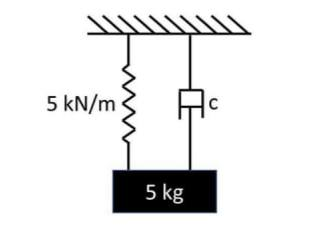
\includegraphics[width=\columnwidth]{2022/AE/62/figs/fig1.png}
\end{figure}

\hfill {(GATE AE-62 (2022))}
\solution
\newpage

\end{enumerate}

\section{2021}
\begin{enumerate}[label=\thechapter.\arabic*,ref=\thechapter.\theenumi]
\item 
\solution
\input{}
\pagebreak
\end{enumerate}

\chapter{Filters}
\section{2022}
\begin{enumerate}[label=\thechapter.\arabic*,ref=\thechapter.\theenumi]
\item The network shown below has a resonant frequency of 150 kHz and bandwidth of 600
Hz. The Q-factor of the network is \rule{1cm}{0.15mm}\\
(rounded off to one decimal place).\\
\hfill(GATE 2022 EC)\\
\begin{figure}[ht]
  \centering
  
      \begin{circuitikz}[american]
    \draw (0,0) to [short, *-] (5,0) to [R=R] (5,2) to [L=L] (5,4) to [short] (2,4) to [C=C] (2,0);
    \draw (0,4) to [short, *-] (2,4);
\end{circuitikz}
  
  \caption{Circuit 1}
\end{figure}\\
\solution\\
\iffalse
\documentclass[journal,12pt,twocolumn]{IEEEtran}
\usepackage{amsmath,amssymb,amsfonts,amsthm}
\usepackage{txfonts}
\usepackage{tkz-euclide}
\usepackage{listings}
\usepackage{gvv}
\usepackage[latin1]{inputenc}
\usepackage{adjustbox}
\usepackage{array}
\usepackage{tabularx}
\usepackage{enumitem}
\usepackage{pgf}
\usepackage{lmodern}
\usepackage{circuitikz}
\usepackage{tikz}
\usepackage{graphicx}


\begin{document}
\bibliographystyle{IEEEtran}

\vspace{3cm}

\title{}
\author{EE23BTECH11054 -  Sai Krishna Shanigarapu$^{*}$
}
\maketitle
\newpage
\bigskip

\section*{Gate EE 2022}
28. \hspace{2pt}The network shown below has a resonant frequency of 150 kHz and bandwidth of 600
Hz. The Q-factor of the network is \rule{1cm}{0.15mm}\\
(rounded off to one decimal place).\\
\hfill(GATE 2022 EC)\\
\begin{figure}[ht]
  \centering
  
      \begin{circuitikz}[american]
    \draw (0,0) to [short, *-] (5,0) to [R=R] (5,2) to [L=L] (5,4) to [short] (2,4) to [C=C] (2,0);
    \draw (0,4) to [short, *-] (2,4);
\end{circuitikz}
  
  \caption{Circuit 1}
\end{figure}\\
\solution
\fi

\begin{figure}[ht]
  \centering
  
      \begin{circuitikz}[american]
    \draw (0,0) to [short, *-] (5,0) to [R=R] (5,2) to [L=$j\omega L$] (5,4) to [short] (2,4) to [C=$\frac{1}{j\omega C}$] (2,0);
    \draw (0,4) to [short, *-] (2,4);
\end{circuitikz}

  \caption{Circuit 2}
\end{figure}


\begin{table}[ht]
    \centering
 
    \setlength{\arrayrulewidth}{0.3mm}
\setlength{\tabcolsep}{20pt}
\renewcommand{\arraystretch}{1.3}


\begin{tabular}{|c|c|c|}
\hline
Parameter & Description & Value\\
\hline
$f_0$ & Resonant frequency & 150 kHz\\
\hline
$B$ & Bandwidth & 600 Hz\\
\hline
\end{tabular}

    \caption{Parameters}
    \label{tab:tab1_gate_ee_2022_28_054}
\end{table}

\begin{table}[ht]
    \centering

    \setlength{\arrayrulewidth}{0.3mm}
\setlength{\tabcolsep}{20pt}
\renewcommand{\arraystretch}{1.5}


\begin{tabular}{|c|c|c|}
\hline
Parameter & Description & Formula\\
\hline
$Q$ & Quality factor & $\frac{X_L}{R}$\\
\hline
$B$ & Bandwidth & $\frac{R}{2 \pi L}$\\
\hline
$\omega_0$ & Radial resonant frequency & $2 \pi f_0$\\
\hline
$X_L$ & Inductive reactance & $\omega L$\\
\hline
$X_C$ & Capacitive reactance & $\frac{1}{\omega C}$\\
\hline

\end{tabular}


    \caption{Formulae}
    \label{tab:tab2_gate_ee_2022_28_054}
\end{table}

At Resonance, 
\begin{align}
    X_L & = X_C\\
    \omega_0 L &= \frac{1}{\omega_0 C}\\
    \omega_0 &= \frac{1}{\sqrt{LC}}\\
    2 \pi f_0 &= \frac{1}{\sqrt{LC}}\\
    \implies f_0 &= \frac{1}{2 \pi \sqrt{LC}} \label{eq:eq1_gate_ee_2022_28_054}    
\end{align}

Using Table \ref{tab:tab2_gate_ee_2022_28_054},
\begin{align}
    Q &= \frac{X_L}{R}\\
    &= \frac{\omega_0 L}{R}\\
    &= \brak{\frac{1}{\sqrt{LC}}}\frac{L}{R}\\
    \implies Q &= \frac{1}{R}\sqrt{\frac{L}{C}} \label{eq:eq2_gate_ee_2022_28_054}
\end{align}

From eq (\ref{eq:eq1_gate_ee_2022_28_054}) and Table \ref{tab:tab2_gate_ee_2022_28_054}
\begin{align}
    \frac{f_0}{B} &= \brak{\frac{1}{2\pi \sqrt{LC}}}\frac{2 \pi L}{R}\\
    &= \brak{\frac{1}{\sqrt{LC}}}\frac{L}{R}\\
    \implies \frac{f_0}{B} &= \frac{1}{R}\sqrt{\frac{L}{C}} \label{eq:eq3_gate_ee_2022_28_054}
\end{align}

From Table \ref{tab:tab1_gate_ee_2022_28_054}, eq (\ref{eq:eq2_gate_ee_2022_28_054}) and eq (\ref{eq:eq3_gate_ee_2022_28_054}),
\begin{align}
    Q &= \frac{f_0}{B}\\
     &=\frac{150 \text{ x } 10^3}{600}\\
    &= 250
\end{align}

$\therefore$ Q-factor is 250

\begin{figure}[ht]
    \centering
    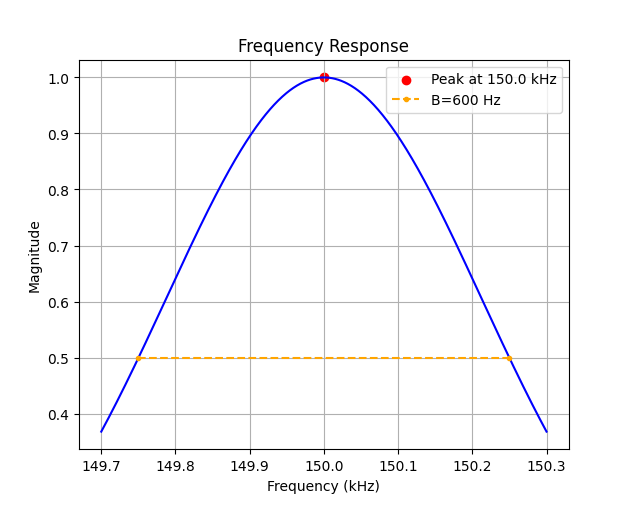
\includegraphics[width=\columnwidth]{2022/EE/28/figs/Figure_1.png}
    \caption{Plot of Q-factor}
    \label{fig:fig1_gate_ee_2022_18_054}
\end{figure}

%\end{document}

\pagebreak
\end{enumerate}

\section{2021}
\begin{enumerate}[label=\thechapter.\arabic*,ref=\thechapter.\theenumi]
\item 
\solution
\input{}
\pagebreak
\end{enumerate}

\chapter{ Z-transform}
\section{2022}
\begin{enumerate}[label=\thechapter.\arabic*,ref=\thechapter.\theenumi]
\item Consider the following recursive iteration scheme for different values of variable P with the initial guess $x_1=1$:
$$x_{n+1}=\frac{1}{2}\brak{x_n+\frac{P}{x_n}}, \quad\quad n=1,2,3,4,5 $$
For $P=2$, $x_5$ is obtained to be 1.414, rounded off to 3 decimal places. For $P=3$, $x_5$ is obtained to be 1.732, rounded off to 3 decimal places.   \\ \\
If $P=10$, the numerical value of $x_5$ is \rule{1.3cm}{0.15mm} . ($round$ $off$ $to$ $three$ $decimal$ $places$)     \hfill(GATE CE 2022) \\
\solution \iffalse
\let\negmedspace\undefined
\let\negthickspace\undefined
\documentclass[journal,12pt,twocolumn]{IEEEtran}
\usepackage{cite}
\usepackage{amsmath,amssymb,amsfonts,amsthm}
\usepackage{algorithmic}
\usepackage{graphicx}
\usepackage{textcomp}
\usepackage{xcolor}
\usepackage{txfonts}
\usepackage{listings}
\usepackage{enumitem}
\usepackage{mathtools}
\usepackage{gensymb}
\usepackage{comment}
\usepackage[breaklinks=true]{hyperref}
\usepackage{tkz-euclide} 
\usepackage{listings}
\usepackage{gvv}                                        
\def\inputGnumericTable{}                                 
\usepackage[latin1]{inputenc}                                
\usepackage{color}                                            
\usepackage{array}                                            
\usepackage{longtable}                                       
\usepackage{calc}                                             
\usepackage{multirow}                                         
\usepackage{hhline}                                           
\usepackage{ifthen}                                           
\usepackage{lscape}

\newtheorem{theorem}{Theorem}[section]
\newtheorem{problem}{Problem}
\newtheorem{proposition}{Proposition}[section]
\newtheorem{lemma}{Lemma}[section]
\newtheorem{corollary}[theorem]{Corollary}
\newtheorem{example}{Example}[section]
\newtheorem{definition}[problem]{Definition}
\newcommand{\BEQA}{\begin{eqnarray}}
\newcommand{\EEQA}{\end{eqnarray}}
\newcommand{\define}{\stackrel{\triangle}{=}}
\theoremstyle{remark}
\newtheorem{rem}{Remark}
\begin{document}
\parindent 0px
\bibliographystyle{IEEEtran}
\title{GATE: CE - 29.2022}
\author{EE22BTECH11219 - Rada Sai Sujan$^{}$% <-this % stops a space
}
\maketitle
\newpage
\bigskip
\section*{Question}
Consider the following recursive iteration scheme for different values of variable P with the initial guess $x_1=1$:
$$x_{n+1}=\frac{1}{2}\brak{x_n+\frac{P}{x_n}}, \quad\quad n=1,2,3,4,5 $$
For $P=2$, $x_5$ is obtained to be 1.414, rounded off to 3 decimal places. For $P=3$, $x_5$ is obtained to be 1.732, rounded off to 3 decimal places.   \\ \\
If $P=10$, the numerical value of $x_5$ is \rule{1.3cm}{0.15mm} . ($round$ $off$ $to$ $three$ $decimal$ $places$)     \hfill(GATE CE 2022) \\
\solution 
\fi

Applying $A.M \geq G.M$ inequality,
\begin{align}
    \frac{x_n+\frac{P}{x_n}}{2} \geq \sqrt{P}   \\
    \implies x_{n+1} \geq \sqrt{P}  \label{eq:ce.29.22.1}
\end{align}
Solving the equation,
\begin{align}
    2x_{n+1}x_{n} - {x_n}^2 - P &=0
\end{align}
Applying $Z$-transform we get,
\begin{align}
    X\brak{z} \ast X\brak{z} &= \frac{PZ^{-1}}{\brak{1-z^{-1}}\brak{2-z^{-1}}}  \\
    &= P\brak{\frac{z^{-1}}{1-z^{-1}} - \frac{z^{-1}}{2-z^{-1}}}
\end{align}
From the transformation pairs,
\begin{align}
    x_{n-a} &\overset{\mathcal{Z}}{ \longleftrightarrow} z^{-a}X\brak{z}  \\
    x_{n_1}\times x_{n_2} &\overset{\mathcal{Z}}{ \longleftrightarrow} X_1\brak{z}\ast X_2\brak{z} \\
    \frac{u\brak{n-1}}{a^{n}} &\overset{\mathcal{Z}}{ \longleftrightarrow} \frac{z^{-1}}{a-z^{-1}}
\end{align}
Now, applying inverse $Z$-tranform,
\begin{align}
    x_n^2 &= P\brak{u\brak{n-1} - \frac{u\brak{n-1}}{2^n}}  \\
    \implies x_n^2 &=P\brak{1-\frac{1}{2^n}} \quad \text{[$\because n \geq 1$]}
\end{align}
Similarly,
\begin{align}
    x_{n+1}^2 &= P\brak{1 - \frac{1}{2^{n+1}}}  \\
    \implies \lim\limits_{n\to\infty}\frac{x_{n+1}}{x_n} &= \lim\limits_{n\to\infty}\sqrt{\frac{P\brak{1-\frac{1}{2^n}}}{P\brak{1-\frac{1}{2^{n+1}}}}}    \\
    &=1
\end{align}
Hence, the system is convergent.    \\
Now finding the limit of the sequence,
\begin{align}
    x^2 &=\lim\limits_{x\to\infty}P\brak{1-\frac{1}{2^n}}   \\
    \implies x &= \pm\sqrt{P}   \label{eq:ce.29.22.11}
\end{align}
From \eqref{eq:ce.29.22.1} and \eqref{eq:ce.29.22.11},
\begin{align}
    x_{n+1}=\sqrt{P}
\end{align}
Therefore, for $P=10$ the value of $x_5$ is,
\begin{align}
    x_5&=\sqrt{10}  \\
    \therefore x_5&=3.162
\end{align}

\newpage
\item The block diagram of a two-tap high-pass FIR filter is shown below. The filter transfer function is given by $H(z) = Y(z)/X(z)$.\\
If the ratio of maximum to minimum value of $H(z)$ is 2 and $\abs{H(z)}_{max} = 1$, the coefficients $\beta_0$ and $\beta_1$ are \underline{\hspace{3cm}} and \underline{\hspace{3cm}}, respectively. 

\begin{figure}[H]
    \centering
    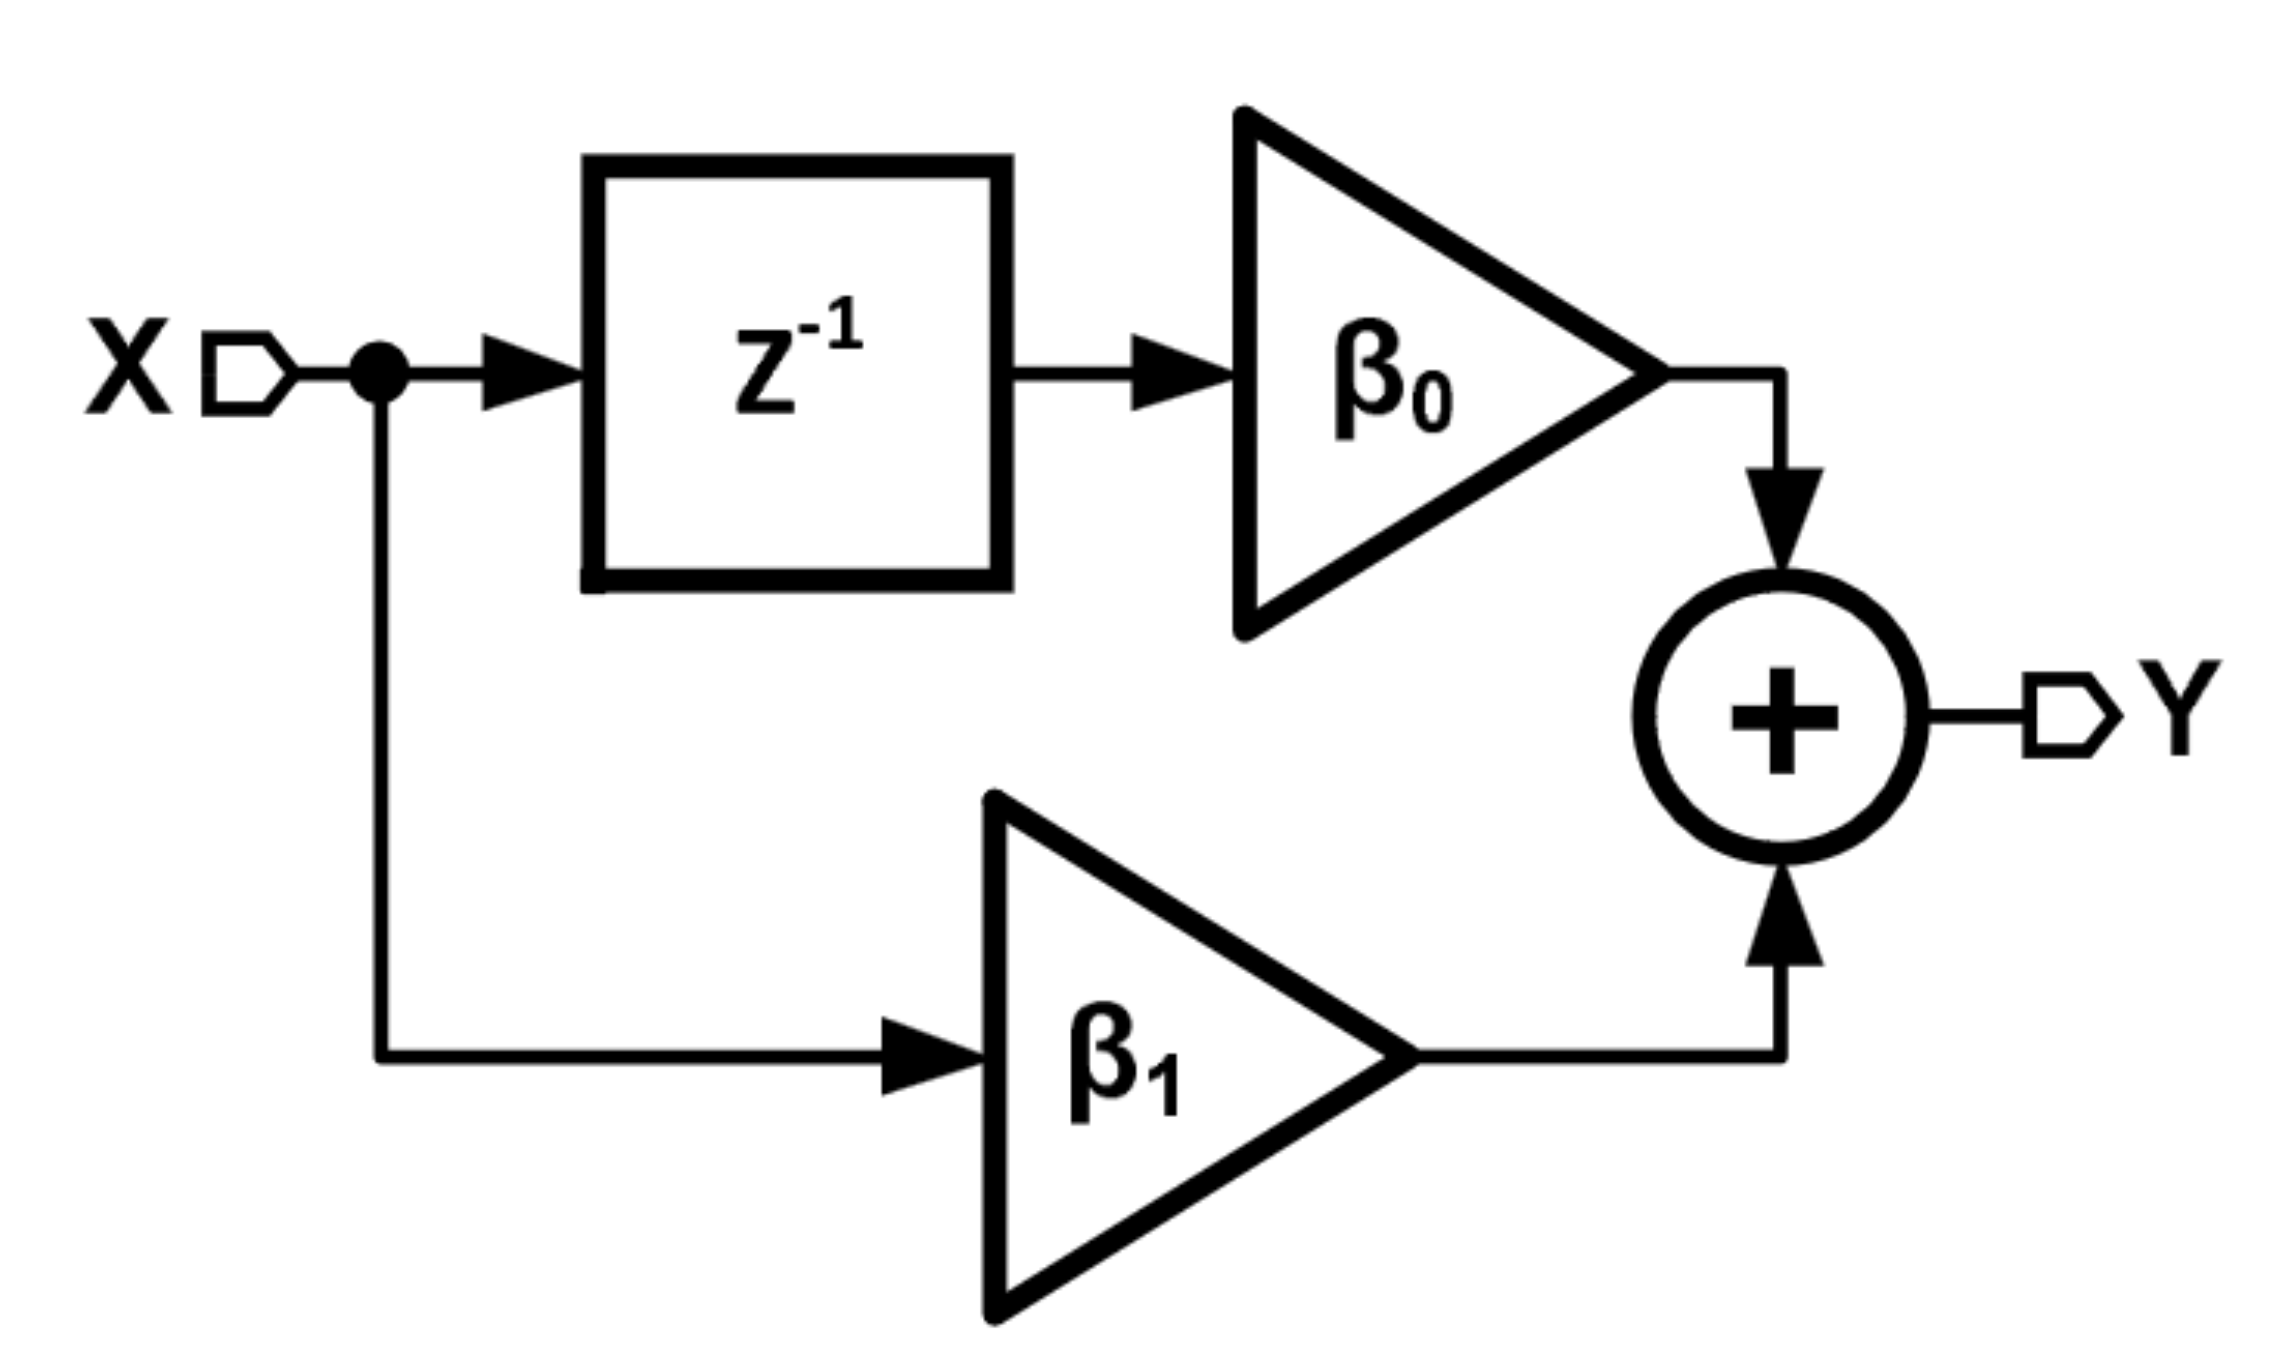
\includegraphics[width=0.5\linewidth]{2022/BM/39/figs/qfig.png} 
    \caption{Block diagram}
    \label{fig:GATE22BM39.1}
\end{figure}


\begin{enumerate}[label=(\Alph*)]
\item 0.75, -0.25
\item 0.67, 0.33
\item 0.60, -0.40
\item -0.64, 0.36
\end{enumerate}
\hfill{GATE BM 2022} \\
\solution \\
\iffalse
\let\negmedspace\undefined
\let\negthickspace\undefined
\documentclass[journal,12pt,onecolumn]{IEEEtran}
\usepackage{cite}
\usepackage{amsmath,amssymb,amsfonts,amsthm}
%\usepackage{algorithmic}
\usepackage{graphicx}
\usepackage{textcomp}
\usepackage{array}
\usepackage{xcolor}
\usepackage{txfonts}
\usepackage{listings}
\usepackage{enumitem}
\usepackage{mathtools}
\usepackage{gensymb}
\usepackage[breaklinks=true]{hyperref}
\usepackage{tkz-euclide} % loads  TikZ and tkz-base
\usepackage{listings}
\usepackage{float}
\usepackage{bm}



\newtheorem{theorem}{Theorem}[section]
\newtheorem{problem}{Problem}
\newtheorem{proposition}{Proposition}[section]
\newtheorem{lemma}{Lemma}[section]
\newtheorem{corollary}[theorem]{Corollary}
\newtheorem{example}{Example}[section]
\newtheorem{definition}[problem]{Definition}
%\newtheorem{thm}{Theorem}[section] 
%\newtheorem{defn}[thm]{Definition}
%\newtheorem{algorithm}{Algorithm}[section]
%\newtheorem{cor}{Corollary}
\newcommand{\BEQA}{\begin{eqnarray}}
\newcommand{\EEQA}{\end{eqnarray}}
\newcommand{\define}{\stackrel{\triangle}{=}}
\theoremstyle{remark}
\newtheorem{rem}{Remark}
%\bibliographystyle{ieeetr}
\begin{document}
%
\providecommand{\pr}[1]{\ensuremath{\Pr\left(#1\right)}}
\providecommand{\prt}[2]{\ensuremath{p_{#1}^{\left(#2\right)} }}        % own macro for this question
\providecommand{\qfunc}[1]{\ensuremath{Q\left(#1\right)}}
\providecommand{\sbrak}[1]{\ensuremath{{}\left[#1\right]}}
\providecommand{\lsbrak}[1]{\ensuremath{{}\left[#1\right.}}
\providecommand{\rsbrak}[1]{\ensuremath{{}\left.#1\right]}}
\providecommand{\brak}[1]{\ensuremath{\left(#1\right)}}
\providecommand{\lbrak}[1]{\ensuremath{\left(#1\right.}}
\providecommand{\rbrak}[1]{\ensuremath{\left.#1\right)}}
\providecommand{\cbrak}[1]{\ensuremath{\left\{#1\right\}}}
\providecommand{\lcbrak}[1]{\ensuremath{\left\{#1\right.}}
\providecommand{\rcbrak}[1]{\ensuremath{\left.#1\right\}}}
\newcommand{\sgn}{\mathop{\mathrm{sgn}}}
\providecommand{\abs}[1]{\left\vert#1\right\vert}
\providecommand{\res}[1]{\Res\displaylimits_{#1}} 
\providecommand{\norm}[1]{\left\lVert#1\right\rVert}
%\providecommand{\norm}[1]{\lVert#1\rVert}
\providecommand{\mtx}[1]{\mathbf{#1}}
\providecommand{\mean}[1]{E\left[ #1 \right]}
\providecommand{\cond}[2]{#1\middle|#2}
\providecommand{\fourier}{\overset{\mathcal{F}}{ \rightleftharpoons}}
\newenvironment{amatrix}[1]{%
  \left(\begin{array}{@{}*{#1}{c}|c@{}}
}{%
  \end{array}\right)
}
%\providecommand{\hilbert}{\overset{\mathcal{H}}{ \rightleftharpoons}}
%\providecommand{\system}{\overset{\mathcal{H}}{ \longleftrightarrow}}
	%\newcommand{\solution}[2]{\textbf{Solution:}{#1}}
\newcommand{\solution}{\noindent \textbf{Solution: }}
\newcommand{\cosec}{\,\text{cosec}\,}
\providecommand{\dec}[2]{\ensuremath{\overset{#1}{\underset{#2}{\gtrless}}}}
\newcommand{\myvec}[1]{\ensuremath{\begin{pmatrix}#1\end{pmatrix}}}
\newcommand{\mydet}[1]{\ensuremath{\begin{vmatrix}#1\end{vmatrix}}}
\newcommand{\myaugvec}[2]{\ensuremath{\begin{amatrix}{#1}#2\end{amatrix}}}
\providecommand{\rank}{\text{rank}}
\providecommand{\pr}[1]{\ensuremath{\Pr\left(#1\right)}}
\providecommand{\qfunc}[1]{\ensuremath{Q\left(#1\right)}}
	\newcommand*{\permcomb}[4][0mu]{{{}^{#3}\mkern#1#2_{#4}}}
\newcommand*{\perm}[1][-3mu]{\permcomb[#1]{P}}
\newcommand*{\comb}[1][-1mu]{\permcomb[#1]{C}}
\providecommand{\qfunc}[1]{\ensuremath{Q\left(#1\right)}}
\providecommand{\gauss}[2]{\mathcal{N}\ensuremath{\left(#1,#2\right)}}
\providecommand{\diff}[2]{\ensuremath{\frac{d{#1}}{d{#2}}}}
\providecommand{\myceil}[1]{\left \lceil #1 \right \rceil }
\newcommand\figref{Fig.~\ref}
\newcommand\tabref{Table~\ref}
\newcommand{\sinc}{\,\text{sinc}\,}
\newcommand{\rect}{\,\text{rect}\,}
%%
%	%\newcommand{\solution}[2]{\textbf{Solution:}{#1}}
%\newcommand{\solution}{\noindent \textbf{Solution: }}
%\newcommand{\cosec}{\,\text{cosec}\,}
%\numberwithin{equation}{section}
%\numberwithin{equation}{subsection}
%\numberwithin{problem}{section}
%\numberwithin{definition}{section}
%\makeatletter
%\@addtoreset{figure}{problem}
%\makeatother

%\let\StandardTheFigure\thefigure
\let\vec\mathbf

\bibliographystyle{IEEEtran}





\bigskip

%\renewcommand{\thefigure}{\theenumi}
%\renewcommand{\thetable}{\theenumi}
%\renewcommand{\theequation}{\theenumi}

Q:  The block diagram of a two-tap high-pass FIR filter is shown below. The filter transfer function is given by $H(z) = Y(z)/X(z)$.\\
If the ratio of maximum to minimum value of $H(z)$ is 2 and $\abs{H(z)}_{max} = 1$, the coefficients $\beta_0$ and $\beta_1$ are \underline{\hspace{3cm}} and \underline{\hspace{3cm}}, respectively. 

\begin{figure}[H]
    \centering
    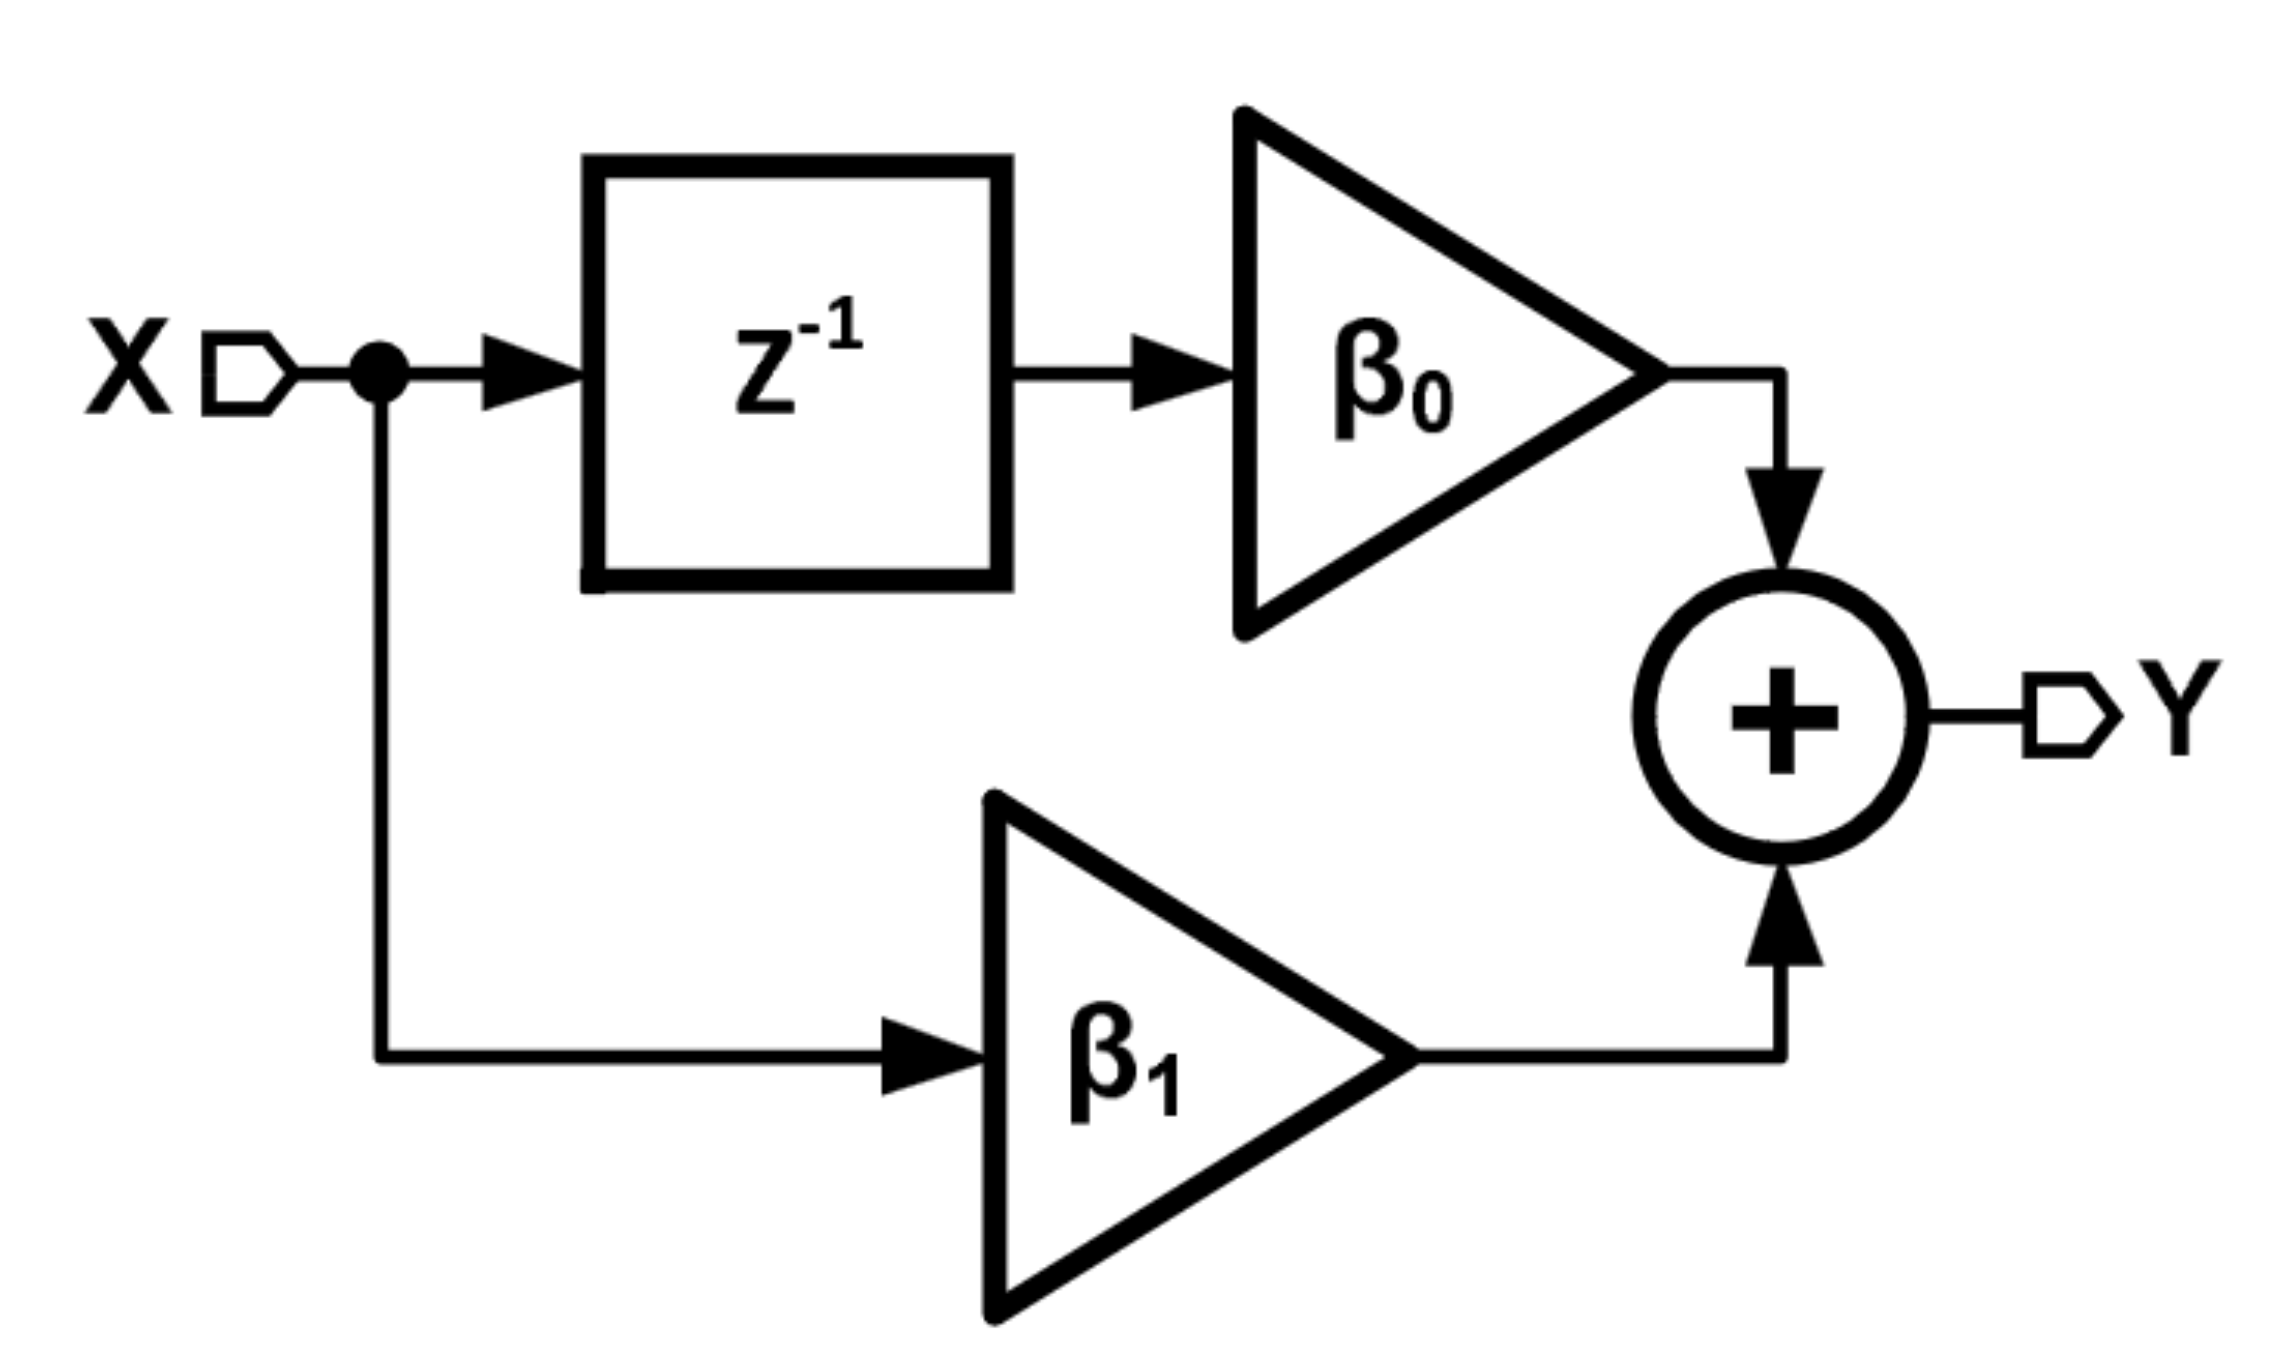
\includegraphics[width=0.5\linewidth]{2022/BM/39/figs/qfig.png} 
    \caption{Block diagram}
    \label{fig:GATE22BM39.1}
\end{figure}


\begin{enumerate}[label=(\Alph*)]
\item 0.75, -0.25
\item 0.67, 0.33
\item 0.60, -0.40
\item -0.64, 0.36
\end{enumerate}
\hfill{GATE BM 2022}


\solution \\
\fi
\textbf{Results and Proofs: \\}
\underline{Time Shift Property:}
\begin{align}
x(n) &\overset{\mathcal{Z}}{\longleftrightarrow} X(z) \\
x(n-n_0) &\overset{\mathcal{Z}}{\longleftrightarrow} z^{-n_0}X(z) 
\end{align}
\underline{Proof:} \\
Let
\begin{align}
y(n) &= x(n-n_0) \label{eq:GATE22BM39.-1}
\end{align}
Taking z-transform
\begin{align}
\mathcal{Z}\brak{y(n)} &= \mathcal{Z}\brak{x(n-n_0)} \label{eq:GATE22BM39.-2}\\
\end{align}
Simplifying LHS
\begin{align}
Y(z) &= \sum_{n=-\infty}^{\infty} y(n)z^{-n} 
\end{align}
From \eqref{eq:GATE22BM39.-1}
\begin{align}
Y(z) &= \sum_{n=-\infty}^{\infty} x(n-n_0) z^{-n} \label{eq:GATE22BM39.-3}
\end{align}
Let 
\begin{align}
n-n_0 &= s  \\\implies
n &= s+n_0 \label{eq:GATE22BM39.-4}
\end{align}
From \eqref{eq:GATE22BM39.-3} and \eqref{eq:GATE22BM39.-4}
\begin{align}
Y(z) &= \sum_{s=-\infty}^{\infty} x(s) z^{-(s+n_0)} \\
&= z^{-n_0}\sum_{s=-\infty}^{\infty} x(s) z^{-s} 
\end{align}
As variable in Z-transform is dummy, on replacing it, we get
\begin{align}
Y(z) &= z^{-n_0}\sum_{n=-\infty}^{\infty} x(n) z^{-n} \\
&= z^{-n_0}X(z) \label{eq:GATE22BM39.-5}
\end{align}
From \eqref{eq:GATE22BM39.-2} and \eqref{eq:GATE22BM39.-5}
\begin{align}
\mathcal{Z}\brak{x(n-n_0)} &= z^{-n_0}X(z)
\end{align}
Hence proved \\
\underline{Result:}
\begin{align}
z^{-n_0}X(z) &\overset{\mathcal{Z^{-}}}{\longleftrightarrow} x(n-n_0) \label{eq:GATE22BM39.-6}
\end{align}
\textbf{Sol:  }
\begin{table}[h]
    \centering
        \begin{tabular}{|c|c|c|} 
      \hline
\textbf{Variable}& \textbf{Description}& \textbf{Value}\\\hline
	 $H(z)$ & Transfer Function & $\beta_0z^{-1} + \beta_1$ \\\hline
         $\abs{H(z)}_{max}$ & Maximum value of Transfer Function & 1 \\\hline  
         $\abs{H(z)}_{min}$ & Minimum value of Transfer Function & $\frac{1}{2}$\\\hline
    \end{tabular}

    \caption{input parameters}
    \label{tab:GATE22BM39.1}
\end{table}
\\In \eqref{eq:GATE22BM39.-6}, put
\begin{align}
n_0 = 1, \quad x(n) = \delta(n) \nonumber 
\end{align}
Since
\begin{align}
1 \overset{\mathcal{Z^{-}}}{\longleftrightarrow} \delta(n) \nonumber
\end{align}
\begin{align}
z^{-1} &\overset{\mathcal{Z^{-}}}{\longleftrightarrow} \delta(n-1)
\end{align}
This is a unit delay in discrete time and represents unit amplitude sinosoidal signal.\\
So,
\begin{align}
z^{-1} &= e^{-jw} \\\implies
\abs{z^{-1}} &= 1 \label{eq:GATE22BM39.1}
\end{align}
Since $H(z)$ is complex, on using Triangle Inequality, we get
\begin{align}
\abs{x + y} \leq \abs{x} + \abs{y} 
\end{align}
And its corollary
\begin{align}
\abs{\abs{x}-\abs{y}} \leq \abs{x + y}
\end{align}
where x and y are complex numbers.
\begin{align}
\abs{\abs{z^{-1}\beta_0}-\abs{\beta_1}} \leq \abs{z^{-1}\beta_0 + \beta_1} \leq \abs{z^{-1}\beta_0} + \abs{\beta_1} 
\end{align}
From \tabref{tab:GATE22BM39.1}
\begin{align}
\abs{\abs{z^{-1}\beta_0}-\abs{\beta_1}} \leq \abs{H(z)} \leq \abs{z^{-1}\beta_0} + \abs{\beta_1}
\end{align}
From \eqref{eq:GATE22BM39.1} 
\begin{align}
\abs{\abs{\beta_0}-\abs{\beta_1}} \leq \abs{H(z)} \leq \abs{\beta_0} + \abs{\beta_1} 
\end{align}
So, we can conclude that
\begin{align}
\abs{H(z)}_{max} &= \abs{\beta_0} + \abs{\beta_1} 
\end{align}
Now from \tabref{tab:GATE22BM39.1}
\begin{align}
1 &= \abs{\beta_0} + \abs{\beta_1} \label {eq:GATE22BM39.2}
\end{align}
Similarly,
\begin{align}
\frac{1}{2} &= \abs{\abs{\beta_0}-\abs{\beta_1}} \label {eq:GATE22BM39.3}
\end{align}
On solving \eqref{eq:GATE22BM39.2} and \eqref{eq:GATE22BM39.3}, we get
\begin{align}
\abs{\beta_0} = 0.75, \abs{\beta_1} = 0.25 
\end{align}
\begin{center}
OR
\end{center}
\begin{align}
\abs{\beta_0} = 0.25, \abs{\beta_1} = 0.75 
\end{align}
Hence the correct answer is option (A) \\




%\end{document}

\pagebreak

\end{enumerate}

\section{2021}
\begin{enumerate}[label=\thechapter.\arabic*,ref=\thechapter.\theenumi]
\item The causal signal with Z transform $z^2(z - a)^{-2}$ is ($u(n)$ is unit step signal)
\begin{enumerate}
    \item $a^{2n}u(n)$
    \item $(n + 1)a^nu(n)$
    \item $n^{-1}a^nu(n)$
    \item $n^2a^nu(n)$
\end{enumerate}

\hfill(GATE 31 EE 2021) 

\solution
 \iffalse
\let\negmedspace\undefined
\let\negthickspace\undefined
\documentclass[journal,12pt,twocolumn]{IEEEtran}
\usepackage{cite}
\usepackage{amsmath,amssymb,amsfonts,amsthm}
\usepackage{algorithmic}
\usepackage{graphicx}
\usepackage{textcomp}
\usepackage{xcolor}
\usepackage{txfonts}
\usepackage{listings}
\usepackage{enumitem}
\usepackage{mathtools}
\usepackage{gensymb}
\usepackage{comment}
\usepackage[breaklinks=true]{hyperref}
\usepackage{tkz-euclide} 
\usepackage{tikz}
% \usetikzlibrary{positioning, arrows.meta}
\usepackage{listings}
\usepackage{gvv} 
\usepackage{caption}
\def\inputGnumericTable{}                   

%\usepackage[latin1]{inputenc}                                
\usepackage{color}                                            
\usepackage{array}                                            
\usepackage{longtable}                                       
\usepackage{calc}                                             
\usepackage{multirow}                                         
\usepackage{hhline}                                           
\usepackage{ifthen}                                           
\usepackage{lscape}
\usepackage{tikz}
\newtheorem{theorem}{Theorem}[section]
\newtheorem{problem}{Problem}
\newtheorem{proposition}{Proposition}[section]
\newtheorem{lemma}{Lemma}[section]
\newtheorem{corollary}[theorem]{Corollary}
\newtheorem{example}{Example}[section]
\newtheorem{definition}[problem]{Definition}
\newcommand{\BEQA}{\begin{eqnarray}}
\newcommand{\EEQA}{\end{eqnarray}}
\newcommand{\define}{\stackrel{\triangle}{=}}
\theoremstyle{remark}
\newtheorem{rem}{Remark}

\begin{document}

\bibliographystyle{IEEEtran}
\vspace{3cm}

\title{GATE: EE - 31.2021}
\author{EE23BTECH11013 - Avyaaz$^{*}$% <-this % stops a space 
}
\maketitle
\newpage
\bigskip

\renewcommand{\thefigure}{\arabic{figure}}
\renewcommand{\thetable}{\arabic{table}}

\large\textbf{\textsl{Question:}}
The causal signal with Z transform $z^2(z - a)^{-2}$ is ($u(n)$ is unit step signal)
\begin{enumerate}
    \item $a^{2n}u(n)$
    \item $(n + 1)a^nu(n)$
    \item $n^{-1}a^nu(n)$
    \item $n^2a^nu(n)$
\end{enumerate}

\hfill(GATE EE 2021) \\
\solution
\fi
% \begin{table}[htbp]
%     \centering
%      \begin{tabular}{|c|c|c|}
\hline
    Parameter & Description & Value\\
    \hline
    $P(s)$ & Plant Transfer Function & $\frac{0.001}{s\brak{\frac{s}{0.5}+1}\brak{\frac{s}{100}+1}}$\\
    \hline
    $C(s)$ & Lag Compensator  & $\frac{100\brak{\frac{s}{10}+1}}{\frac{s}{0.1}+1}$\\
    \hline
    $T(s)$ & Loop gain  & $P(s) C(s)$ \\
    \hline
    $\omega$ & Angular Frequency & 3rad/s \\
    \hline
\end{tabular}

%     \caption{}
%     \label{tab:my_label.41.IN.2022}
% \end{table}

% \begin{figure}[!htbp]
%     \resizebox{0.501\textwidth}{!}{\documentclass{standalone}
\usepackage{tikz}
\usepackage{graphicx} % For rotatebox
\usetikzlibrary{circuits.ee.IEC}

\begin{document}
\begin{tikzpicture}[circuit ee IEC, scale=0.8, transform shape]

% Define components
\def\kone{2} % Capacitance 1/k1
\def\ktwo{3} % Capacitance 1/k2
\def\lone{1.5} % Inductance L1

% Draw parallel combination
\draw[fill=gray!30] (0,0) to [capacitor={info={$\frac{1}{k_1}$}}] ++(1.5,0) coordinate (C1)
            to [inductor={info'={$L_1$}, swap}] ++(1.5,0) coordinate (L1);

% Add parallel combination with L2 and 1/k2
\draw[fill=gray!30] (C1) ++(1.5,0) to [capacitor={info={\rotatebox{90}{$\frac{1}{k_2}$}}}] ++(0,-1.5) coordinate (C2);
\draw[fill=gray!30] (C2) ++(2,1.5) to [inductor={info'={\rotatebox{90}{$L_2$}}, swap}] ++(0,-1.5) coordinate (L2);

% Join L1 and L2 with a solid line
\draw (0,-1.5) -- (L2);
\draw (0,0) -- (0,-1.5);
\draw (3,0) --(5,0);

% Add pointer and label for i1
\draw[postaction={decorate,decoration={markings,mark=at position 0.5 with {\arrow{>}}}}] (0,0) -- node[above] {\(i_1\)} (0.5,0);

% Add pointer and label for i2
\draw[postaction={decorate,decoration={markings,mark=at position 0.5 with {\arrow{>}}}}] (3,0) -- node[above] {\(i_2\)} (3.5,0);

\end{tikzpicture}
\end{document}

}
%     \caption{Block Diagram of System}
%     \label{fig:gate_IN_Q41_blockdiagram}
% \end{figure}


Z-transform of a causal signal is, 
\begin{align}
    X(z) = z^2(z - a)^{-2} = \frac{1}{(1 - az^{-1})^2};|z| > |a|\label{eq:given.EE.31.2021}
\end{align}
The Z transform pair for $a^nu(n)$ signal is given by :
\begin{align}
    a^nu(n) \longleftrightarrow \frac{1}{1 - az^{-1}}
\end{align}
Using differentiation in z-domain property:
\begin{align}
    na^nu(n) &\longleftrightarrow -z\frac{d}{dz}\left(\frac{1}{1 - az^{-1}}\right) \\
     \implies    na^nu(n) &\longleftrightarrow \frac{az^{-1}}{(1 - az^{-1})^2}
\end{align}
Using time-shifting property:
\begin{align}
  (n + 1)a^{n + 1}u(n + 1) \longleftrightarrow \frac{az^{-1}}{(1 - az^{-1})^2}z\\
  (n + 1)a^nu(n + 1) \longleftrightarrow \frac{1}{(1 - az^{-1})^2}\label{EQ:TIME.31.EE.2021}
\end{align}
From \eqref{eq:given.EE.31.2021} and \eqref{EQ:TIME.31.EE.2021}, Inverse Z transform is :
\begin{align}
    x(n) = (n + 1)a^nu(n + 1)
\end{align}
Sequence \(u(n + 1)\) exist for\(-1 \leq n < \infty\), but the factor \((n + 1)\) is zero for \(n = -1\), so \(x(n)\) may be expressed as a causal sequence. 
\begin{align}
    x(n) = (n + 1)a^nu(n)
\end{align}



\begin{figure}[htbp]
    \centering
    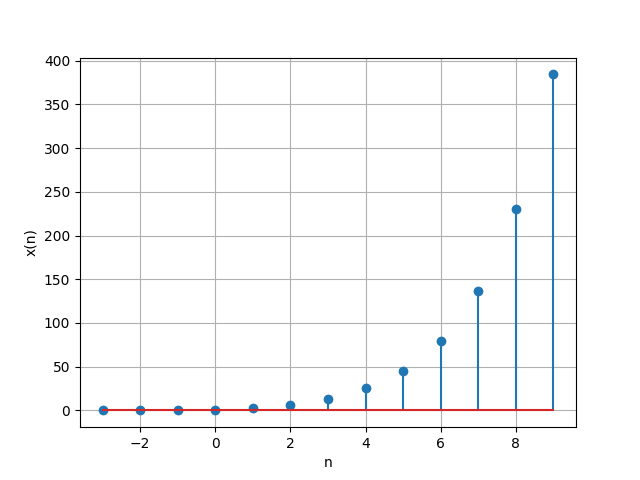
\includegraphics[width = \columnwidth]{2021/EE/31/figs/transform.png}
	\caption{$x(n) vs n $ using $a = 1.5$}
    \label{fig:graph1.41.IN.2022}
\end{figure}


\pagebreak
\end{enumerate}

\chapter{Systems}
\section{2022}
\begin{enumerate}[label=\thechapter.\arabic*,ref=\thechapter.\theenumi]

\item The damping ratio and undamped natural frequency of a closed loop system as
shown in the figure, are denoted as $\zeta$ and $\omega_n$, respectively. The values of $\zeta$ and $\omega_n$
are 
\begin{figure}[!ht]
\centering
\begin{center}
\includegraphics[width=\columnwidth]{2022/EE/39/figs/question.jpg}
\end{center}
%\caption{Diagram for GATE ME Question 30}
\end{figure}
\begin{enumerate}
    \item $\zeta = 0.5$ and $\omega_n = 10$ rad/s
    \item $\zeta = 0.1$ and $\omega_n = 10$ rad/s
    \item $\zeta = 0.707$ and $\omega_n = 10$ rad/s
    \item $\zeta = 0.707$ and $\omega_n = 100$ rad/s
\end{enumerate}
\hfill(GATE EE 2022)
\solution
\iffalse
\let\negmedspace\undefined
\let\negthickspace\undefined
\documentclass[journal,12pt,twocolumn]{IEEEtran}
\usepackage{cite}
\usepackage{amsmath,amssymb,amsfonts,amsthm}
\usepackage{algorithmic}
\usepackage{graphicx}
\usepackage{textcomp}
\usepackage{xcolor}
\usepackage{txfonts}
\usepackage{listings}
\usepackage{enumitem}
\usepackage{mathtools}
\usepackage{gensymb}
\usepackage{comment}
\usepackage[breaklinks=true]{hyperref}
\usepackage{tkz-euclide} 
\usepackage{listings}
\usepackage{gvv}                                        
\def\inputGnumericTable{}                                 
\usepackage[latin1]{inputenc}                                
\usepackage{color}                                            
\usepackage{array}                                            
\usepackage{longtable}                                       
\usepackage{calc}                                             
\usepackage{multirow}                                         
\usepackage{hhline}                                           
\usepackage{ifthen}                                           
\usepackage{lscape}
\usepackage{placeins}
\usepackage{xparse}


\newtheorem{theorem}{Theorem}[section]
\newtheorem{problem}{Problem}
\newtheorem{proposition}{Proposition}[section]
\newtheorem{lemma}{Lemma}[section]
\newtheorem{corollary}[theorem]{Corollary}
\newtheorem{example}{Example}[section]
\newtheorem{definition}[problem]{Definition}
\newcommand{\BEQA}{\begin{eqnarray}}
\newcommand{\EEQA}{\end{eqnarray}}
\newcommand{\define}{\stackrel{\triangle}{=}}
\theoremstyle{remark}
\newtheorem{rem}{Remark}

\graphicspath{ {./figs/} } 

\begin{document}

\bibliographystyle{IEEEtran}
\vspace{3cm}

\Large\title{GATE 2022 EE 39}
\large\author{EE23BTECH11032 - Kaustubh Parag Khachane $^{*}$% <-this % stops a space
}
\maketitle
\newpage
\bigskip

\renewcommand{\thefigure}{\theenumi}
\renewcommand{\thetable}{\theenumi}
\large\textbf{Question GATE 22 EE 39} :\\
The damping ratio and undamped natural frequency of a closed loop system as
shown in the figure, are denoted as $\zeta$ and $\omega_n$, respectively. The values of $\zeta$ and $\omega_n$
are 
\begin{figure}[!ht]
\centering
\begin{center}
\includegraphics[width=\columnwidth]{question}
\end{center}
%\caption{Diagram for GATE ME Question 30}
\end{figure}
\begin{enumerate}
    \item $\zeta = 0.5$ and $\omega_n = 10$ rad/s
    \item $\zeta = 0.1$ and $\omega_n = 10$ rad/s
    \item $\zeta = 0.707$ and $\omega_n = 10$ rad/s
    \item $\zeta = 0.707$ and $\omega_n = 100$ rad/s
\end{enumerate}
\hfill(GATE EE 2022)\\
\solution\\
\fi
\begin{table}[!ht] 
\centering
\setlength{\extrarowheight}{8pt}
\begin{tabular}{|l|l|l|}
    \hline
    \textbf{Parameter} & \textbf{Description} & \textbf{Values}\\
    \hline
     m & load of system &  \\
    \hline
     k & stiffness of system &  \\
    \hline
     $\omega_n$ & Natural frequency & $\sqrt{\frac{k}{m}}$ \\
    \hline
    $\zeta$ & Damping ratio & $\frac{c}{2m\omega_n}$ \\
    \hline
     y\brak{t} & Output of system & \\
    \hline
     x\brak{t} & Input to the system & \\
    \hline
     c & Damping coefficient & \\
    \hline
    T\brak{s} & Transfer function of system & $\frac{Y\brak{s}}{R\brak{s}}$\\
    \hline
  \end{tabular}
  \vspace{4mm}
 \caption{Parameter Table}
 \label{tab:table0_ee_22_39}
\end{table}

We will use Mason's Gain Formula to calculate the transfer function of this system. First converting the given diagram to a signal flow graph :

\begin{figure}[!ht]
\centering
\resizebox{0.5\textwidth}{!}{%
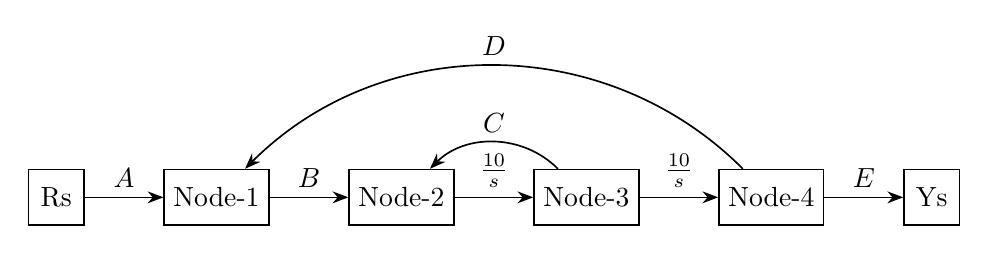
\begin{tikzpicture}[>=Stealth,auto,node distance=1cm,semithick]
  \tikzstyle{block}=[draw, fill=white, rectangle, minimum height=2em, minimum width=2em]
  
  \node [block] (input) {R\brak{s}};
  \node [block, right=of input] (filter) {Node-1};
  \node [block, right=of filter] (D) {Node-2};
  \node [block, right=of D] (E) {Node-3};
  \node [block, right=of E] (F) {Node-4};
  \node [block, right=of F] (output) {Y\brak{s}};
  
  \draw [->] (input) -- node {$A$} (filter);
  \draw [->] (filter) -- node {$B$} (D);
  \draw [->] (D) -- node {$\frac{10}{s}$} (E);
  \draw [->] (E) -- node {$\frac{10}{s}$} (F);
  \draw [->] (F) -- node {$E$} (output);
  
  % Backward loops
  \draw [->] (E) edge [bend right=45] node[above] {$C$} (D);
  \draw [->] (F) edge [bend right=45] node[above] {$D$} (filter);
\end{tikzpicture}%
}
\caption{Signal Flow Diagram}
\label{fig:your_label}
\end{figure}


Mason's Gain Formula is given by :
\begin{align}
    H\brak{s} = \sum_{i=1}^{N}\brak{\frac{P_i \Delta_i}{\Delta}} \label{eq:eq1_ee39}
\end{align}
\begin{table}[!ht] 
\centering
\setlength{\extrarowheight}{8pt}
\begin{tabular}{|l|l|}
    \hline
    \textbf{Parameter} & \textbf{Description}\\
    \hline
     N & Number of forward paths \\\hline
     L & Number of loops\\\hline
     $P_k$ & Forward path gain of $k^{th}$ path\\\hline
     $\Delta_k$ & Associated path factor \\\hline
     $\Delta$ & Determinant of the graph \\\hline
  \end{tabular}
  \vspace{4mm}
 \caption{Parameter Table - Mason's Gain Law}
 \label{tab:table1_ee_22_39}
\end{table}

\begin{table}[!ht] 
\centering
\setlength{\extrarowheight}{8pt}
\begin{tabular}{|l|l|}
    \hline
    \textbf{Parameter} & \textbf{Formula}\\
    \hline
     $\Delta$ & 1 + $\sum_{k=1}^{L}\brak{\brak{-1}^k\text{Product of gain of groups of k isolated loops}}$ \\\hline
     $\Delta_k$ & $\Delta$ part of graph that is not touching $k^{th}$ forward path \\\hline
  \end{tabular}
  \vspace{4mm}
 \caption{Formula Table - Mason's Gain Law}
 \label{tab:table2_ee_22_39}
\end{table}

This signal flow graph has only one forward path whose gain is given by :
\begin{align}
    P_1 &= \frac{10}{s} \frac{10}{s}\\
    &= \frac{100}{s^2}
\end{align}
The loop gain for loop between Node-2 and Node-3 is :
\begin{align}
    L_1 &= \frac{10}{s}\brak{-1}\\
    &= -\frac{10}{s}
\end{align}
The loop gain for loop between Node-1 and Node-4 is :
\begin{align}
    L_1 &= \frac{10}{s}\frac{10}{s}\brak{-1}\\
    &= -\frac{100}{s^2}
\end{align}
Using \tabref{tab:table2_ee_22_39}, $\Delta$ is :
\begin{align}
    \Delta &= 1 - \brak{-\frac{10}{s} - \frac{100}{s^2}}\\
    &= 1 + \frac{10}{s} + \frac{100}{s^2}
\end{align}
There are no two isolated loops available. Hence all further terms will b zero.\\
As both the loops are in contact with the only forward path,
\begin{align}
    \Delta_1 = 1
\end{align}
Using equation \eqref{eq:eq1_ee39} :
\begin{align}
    H\brak{s} &= \frac{\frac{100}{s^2}}{1 + \frac{10}{s} + \frac{100}{s^2}} \\
    &= \frac{100}{s^2 + 10s + 100}\label{eq:eq2_ee39}
\end{align}
Referring to \tabref{tab:table0_ee_22_39}, the general equation of the damping system is second order and can be written as :
\begin{align}
    m\ddot{y}(t) + c\dot{y}(t) + ky(t) = x(t)
\end{align}
Take the Laplace transform and solve for $\frac{Y\brak{s}}{X\brak{s}}$ :
\begin{align}
    \frac{Y\brak{s}}{X\brak{s}} &= \frac{\omega_n^2}{s^2 + 2\zeta\omega_n s + \omega_n^2}\\
\implies H\brak{s} &= \frac{\omega_n^2}{s^2 + 2\zeta\omega_n s + \omega_n^2} \label{eq:eq3_ee39}
\end{align}
Comparing equations \eqref{eq:eq2_ee39} and \eqref{eq:eq3_ee39} ,
\begin{align}
    \omega_n ^2 &= 100\\
    \implies \omega_n &= 10 \text{ rad/s} \label{eq:eq4_ee39}\\
    2\zeta \omega_n &= 10\\
    \implies \zeta &= 0.5
\end{align}
\begin{figure}[!ht]
\centering
\begin{center}
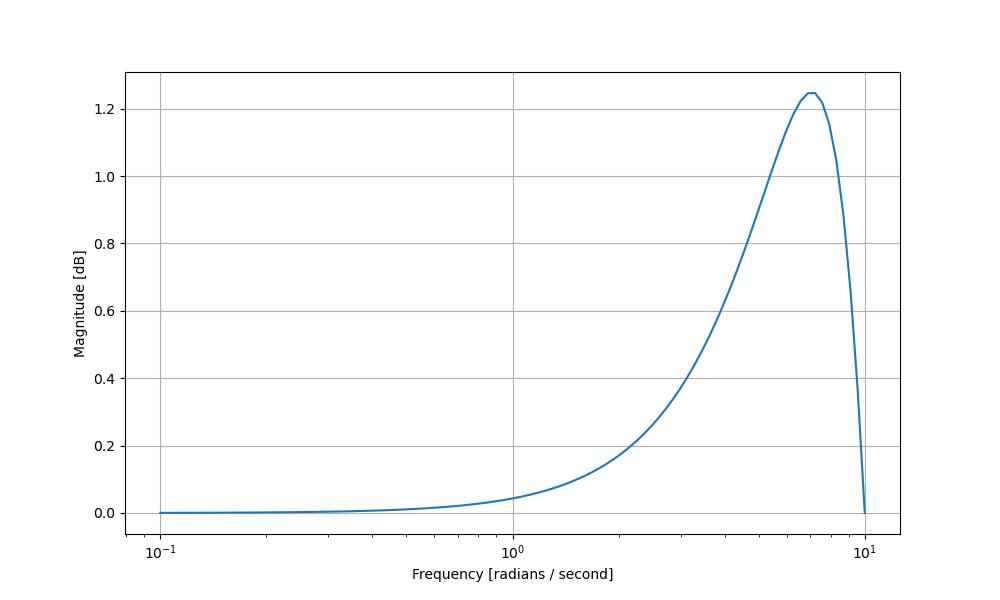
\includegraphics[width=\columnwidth]{2022/EE/39/figs/Figure_1.jpg}
\end{center}
\caption{Magnitude plot}
\end{figure}
\begin{figure}[!ht]
\centering
\begin{center}
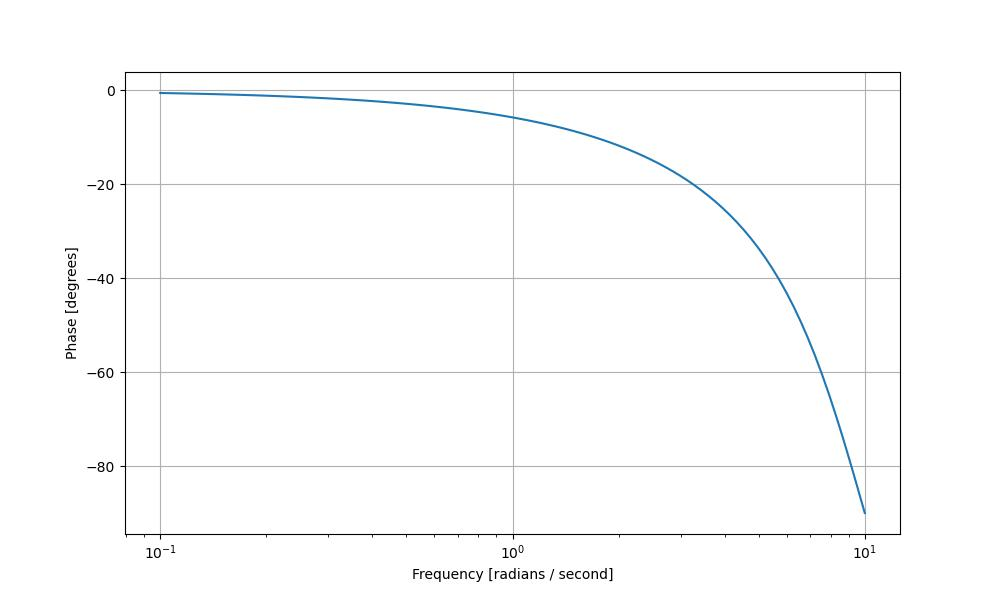
\includegraphics[width=\columnwidth]{2022/EE/39/figs/Figure_2.jpg}
\end{center}
\caption{Phase plot}
\end{figure}

\newpage
\end{enumerate}

\section{2021}
\begin{enumerate}[label=\thechapter.\arabic*,ref=\thechapter.\theenumi]
\item Two discrete-time linear time-invarient systems with impulse responses $h_1[n]=\delta[n-1]+\delta[n+1]$ and $h_2[n]=\delta[n]+\delta[n-1]$ are connected in cascade, where $\delta[n]$ is the Kronecker delta. The impulse response of the cascaded system is   \\
\begin{enumerate}[label=(\alph*)]
    \item $\delta[n-2]+\delta[n+1]$
    \item $\delta[n-1]\delta[n]+\delta[n+1]\delta[n-1]$
    \item $\delta[n-2]+\delta[n-1]+\delta[n]+\delta[n+1]$
    \item $\delta[n]\delta[n-1]+\delta[n-2]\delta[n+1]$
\end{enumerate} \hfill(GATE 2021 EE)\\
\solution
\iffalse
\let\negmedspace\undefined
\let\negthickspace\undefined
\documentclass[journal,12pt,twocolumn]{IEEEtran}
\usepackage{cite}
\usepackage{amsmath,amssymb,amsfonts,amsthm}
\usepackage{algorithmic}
\usepackage{graphicx}
\usepackage{textcomp}
\usepackage{xcolor}
\usepackage{pgfplots}
\usepackage{txfonts}
\usepackage{listings}
\usepackage{enumitem}
\usepackage{mathtools}
\usepackage{gensymb}
\usepackage{comment}
\usepackage[breaklinks=true]{hyperref}
\usepackage{tkz-euclide} 
\usepackage{listings}
\usepackage{gvv}                                        
\def\inputGnumericTable{}                                 
\usepackage[latin1]{inputenc}                                
\usepackage{color}                                            
\usepackage{array}                                            
\usepackage{longtable}                                       
\usepackage{calc}                                             
\usepackage{multirow}                                         
\usepackage{hhline}                                           
\usepackage{ifthen}                                           
\usepackage{lscape}

\newtheorem{theorem}{Theorem}[section]
\newtheorem{problem}{Problem}
\newtheorem{proposition}{Proposition}[section]
\newtheorem{lemma}{Lemma}[section]
\newtheorem{corollary}[theorem]{Corollary}
\newtheorem{example}{Example}[section]
\newtheorem{definition}[problem]{Definition}
\newcommand{\BEQA}{\begin{eqnarray}}
\newcommand{\EEQA}{\end{eqnarray}}
\newcommand{\define}{\stackrel{\triangle}{=}}
\theoremstyle{remark}
\newtheorem{rem}{Remark}
\begin{document}
\parindent 0px
\bibliographystyle{IEEEtran}
\title{GATE: EE - 7.2021}
\author{EE22BTECH11219 - Rada Sai Sujan$^{}$% <-this % stops a space
}
\maketitle
\newpage
\bigskip
\section*{Question}
Two discrete-time linear time-invarient systems with impulse responses $h_1[n]=\delta[n-1]+\delta[n+1]$ and $h_2[n]=\delta[n]+\delta[n-1]$ are connected in cascade, where $\delta[n]$ is the Kronecker delta. The impulse response of the cascaded system is   \\
\begin{enumerate}[label=(\alph*)]
    \item $\delta[n-2]+\delta[n+1]$
    \item $\delta[n-1]\delta[n]+\delta[n+1]\delta[n-1]$
    \item $\delta[n-2]+\delta[n-1]+\delta[n]+\delta[n+1]$
    \item $\delta[n]\delta[n-1]+\delta[n-2]\delta[n+1]$
\end{enumerate} \hfill(GATE 2021 EE)\\
\solution
\fi

\begin{figure}[ht]
    \centering
    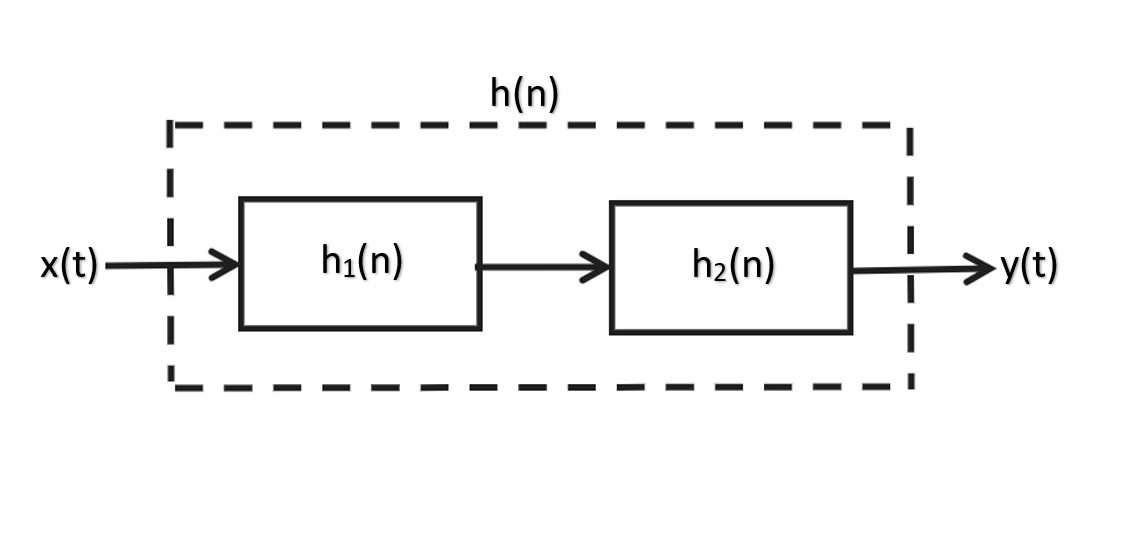
\includegraphics[width=\columnwidth]{2021/EE/7/figs/fig2.png}
    \caption{Block Diagram}
    \label{fig:g2022ee7.2}
\end{figure}  
From the $Z$-transformation pairs,
\begin{align}
    \delta[n] &\overset{\mathcal{Z}}{ \longleftrightarrow} 1  \label{eqn:g22ee7.1}  \\
    x\brak{n-k} &\overset{\mathcal{Z}}{ \longleftrightarrow} z^{-k}X\brak{z} \label{eqn:g22ee7.2}   \\
    x_1\brak{n}\ast x_2\brak{n} &\overset{\mathcal{Z}}{ \longleftrightarrow} X_1\brak{z}X_2\brak{z} \label{eqn:g22ee7.3}
\end{align}
If $h_1\brak{n}$ and $h_2\brak{n}$ are cascade connected then the resultant impulse can be given by:
\begin{align}
    h\brak{n}&=h_1\brak{n}\ast h_2\brak{n}    \\
    \implies H\brak{z}&=H_1\brak{z}H_2\brak{z}    \\
    H\brak{z}&=\brak{z^{-1}+z}\brak{1+z^{-1}}   \\
    &=\brak{z^{-1}+z^{-2}+z+1}, \quad \abs{z}\neq 0
\end{align}
Using the $Z$-transformation pairs to find the the inverse $Z$-transform,
\begin{align}
    h\brak{n}&=\delta[n-2]+\delta[n-1]+\delta[n]+\delta[n+1]
\end{align}
\begin{figure}[ht]
    \centering
    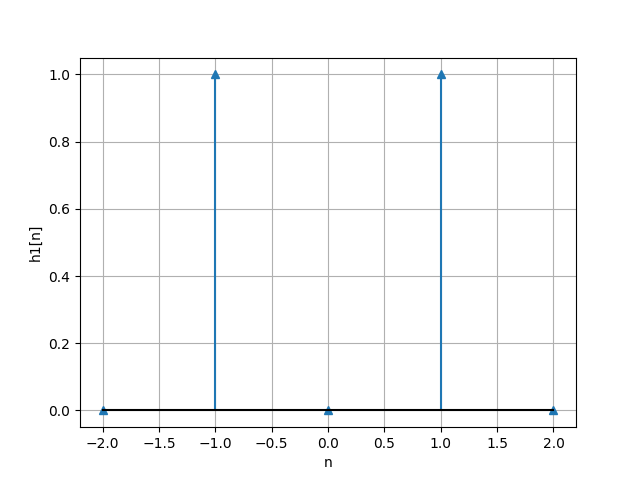
\includegraphics[width=\columnwidth]{2021/EE/7/figs/fig3.png}
    \caption{$h_1\brak{n}$ $vs$ $n$ graph}
    \label{fig:g2022ee7.3}
\end{figure}     
\begin{figure}[ht]
    \centering
    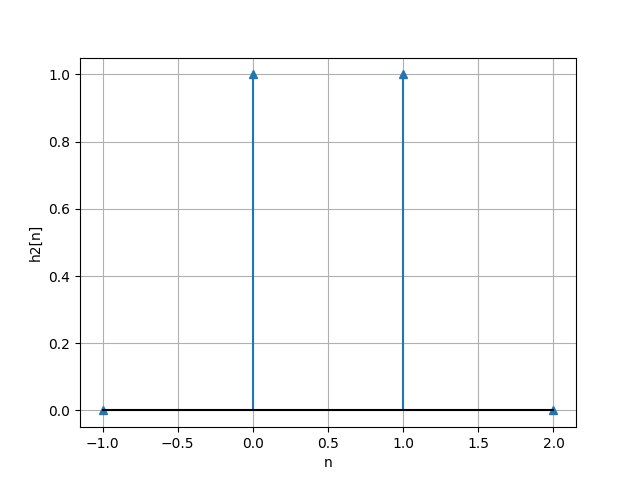
\includegraphics[width=\columnwidth]{2021/EE/7/figs/fig4.png}
    \caption{$h_2\brak{n}$ $vs$ $n$ graph}
    \label{fig:g2022ee7.4}
\end{figure}     
\begin{figure}[ht]
    \centering
    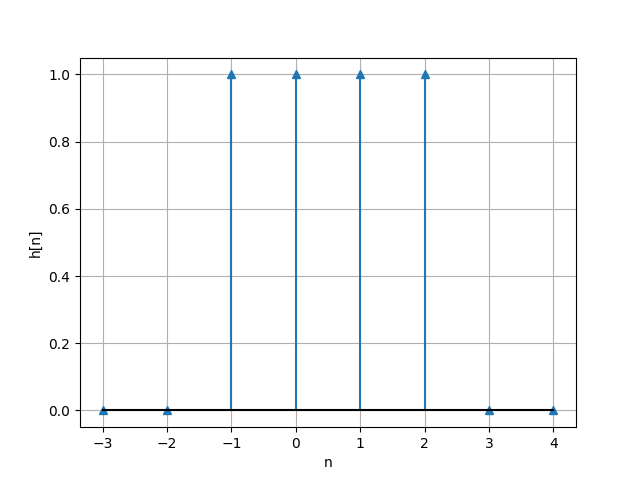
\includegraphics[width=\columnwidth]{2021/EE/7/figs/fig1.png}
    \caption{$h\brak{n}$ $vs$ $n$ graph}
    \label{fig:g2022ee7.1}
\end{figure}

\pagebreak

\item In the given figure, plant $G_p(s)=\frac{2.2}{(1+0.1s)(1+0.4s)(1+1.2s)}$ and compensator $G_c(s)=K\brak{\frac{1+T_1s}{1+T_2s}}$ . The external disturbance input is D(s). It is desired that when the disturbance is a unit step, the steady-state error should not exceed 0.1 unit. The minimum value of K is
\begin{figure}[h!]
    \centering
    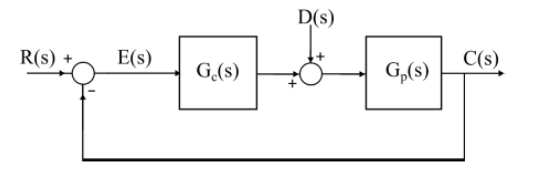
\includegraphics[width=\columnwidth]{2021/EE/47/figs/fig.png}
    \caption{}
    \label{fig:sr47}
\end{figure}
\solution
\iffalse
\documentclass[journal,12pt,twocolumn]{IEEEtran}
\usepackage{cite}
\usepackage{amsmath,amssymb,amsfonts,amsthm}
\usepackage{algorithmic}
\usepackage{graphicx}
\usepackage{textcomp}
\usepackage{xcolor}
\usepackage{txfonts}
\usepackage{listings}
\usepackage{enumitem}
\usepackage{mathtools}
\usepackage{float}
\usepackage{gensymb}
\usepackage{comment}
\usepackage[breaklinks=true]{hyperref}
\usepackage{tkz-euclide} 
\usepackage{listings}
\usepackage{gvv}                                        
\def\inputGnumericTable{}                                 
\usepackage[latin1]{inputenc}                                
\usepackage{color}                                            
\usepackage{array}                                            
\usepackage{longtable}                                       
\usepackage{calc}                                             
\usepackage{multirow}                                         
\usepackage{hhline}                                           
\usepackage{ifthen}                                           
\usepackage{lscape}
\usepackage{amsmath}
\newtheorem{theorem}{Theorem}[section]
\newtheorem{problem}{Problem}
\newtheorem{proposition}{Proposition}[section]
\newtheorem{lemma}{Lemma}[section]
\newtheorem{corollary}[theorem]{Corollary}
\newtheorem{example}{Example}[section]
\newtheorem{definition}[problem]{Definition}
\newcommand{\BEQA}{\begin{eqnarray}}
\newcommand{\EEQA}{\end{eqnarray}}
\newcommand{\define}{\stackrel{\triangle}{=}}
\theoremstyle{remark}
\newtheorem{rem}{Remark}

\usepackage{circuitikz} 

\begin{document}
{\small

\bibliographystyle{IEEEtran}
\vspace{3cm}

\title{GATE 2021 EE 47}
\author{EE23BTECH11045 - Palavelli Srija$^{*}$}

\maketitle

\bigskip

\renewcommand{\thefigure}{\theenumi}
\renewcommand{\thetable}{\theenumi}

\vspace{3cm}
\textbf{Question:} 
In the given figure, plant $G_p(s)=\frac{2.2}{(1+0.1s)(1+0.4s)(1+1.2s)}$ and compensator $G_c(s)=K\brak{\frac{1+T_1s}{1+T_2s}}$ . The external disturbance input is D(s). It is desired that when the disturbance is a unit step, the steady-state error should not exceed 0.1 unit. The minimum value of K is
\begin{figure}[h!]
    \centering
    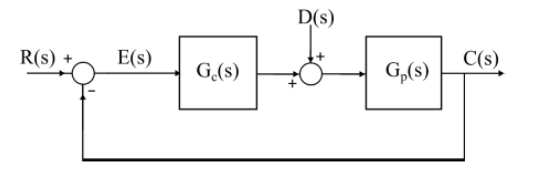
\includegraphics[width=\columnwidth]{2021/EE/47/figs/fig.png}
    \caption{}
    \label{fig:sr40}
\end{figure}
\\
\textbf{Solution:}\\
\fi
\begin{table}[h!]
    \centering
     \begin{tabular}{|c|c|}
        \hline
        \textbf{Symbol}  & \textbf{Value} \\
        \hline
        $G_p(s)$ & $\frac{2.2}{(1+0.1s)(1+0.4s)(1+1.2s)}$\\
         \hline
        $G_c(s)$& $K\brak{\frac{1+T_1s}{1+T_2s}}$  \\
         \hline
        $|e_{ss}|$& $\leq 0.1$\\
         \hline
        $K_{min}$& ??\\
        \hline
    \end{tabular}

    \caption{Input Parameters}
    \label{tab:table_omega}
\end{table}
 
\begin{align}
\text{From \figref{fig:sr40}}\notag\\
E(s) &= R(s)-C(s) \\
\text{Assume R(s)=0}\notag\\
E(s) &= -C(s) \\
C(s) &= \brak{E(s)G_c(s)+D(s)}G_p(s) \\
-E(s) &= \brak{E(s)G_c(s)+D(s)}G_p(s) \\
E(s) &= \frac{-D(s)G_p(s)}{1+G_c(s)G_p(s)} 
\end{align}
Using final value theorem 
\begin{align}
e_{ss} &= \lim_{{t \to \infty}} e(t) = \lim_{{s \to 0}} sE(s)\\
\text{Where}\quad\mathcal{L}\{e(t)\} &= E(s) \notag\\
e_{ss} &= \lim_{{s \to 0}} sE(s) \\
&= \lim_{{s \to 0}} \left(\frac{-sD(s)G_p(s)}{1+G_c(s)G_p(s)} \right) \\
\end{align}
\begin{align}
 D(s)&=\mathcal{L}\{u(t)\}  \notag\\
&=\frac{1}{s}\\
e_{ss} &=\lim_{{s \to 0}} \left(\frac{-s\frac{1}{s}G_p(s)}{1+G_c(s)G_p(s)} \right) \\
&= \lim_{{s \to 0}} \frac{\frac{-2.2}{(1+0.1s)(1+0.4s)(1+1.2s)}}{1+K\left(\frac{1+T_1s}{1+T_2s}\right)\frac{2.2}{(1+0.1s)(1+0.4s)(1+1.2s)}} \\
&= \lim_{{s \to 0}} \frac{-2.2(1+T_2s)}{(1+0.1s)(1+0.4s)(1+1.2s)(1+T_2s)+2.2K(1+T_1s)} \\
|e_{ss}| &= \frac{2.2}{1+2.2K} \\
\text{given}\notag\\ |e_{ss}|&\leq 0.1\\
\frac{2.2}{1+2.2K} &\leq 0.1 \\
K &\geq 9.54 \\
K_{\text{min}} &= 9.54
\end{align}
    %\end{document}

\pagebreak
\end{enumerate}

\chapter{Sequences}
\section{2022}
\begin{enumerate}[label=\thechapter.\arabic*,ref=\thechapter.\theenumi]

\item Discrete signals $x\brak{n}$ and $y\brak{n}$ are shown below. The cross-correlation $r_{xy}\brak{0}$ is:
\begin{figure}[H]
    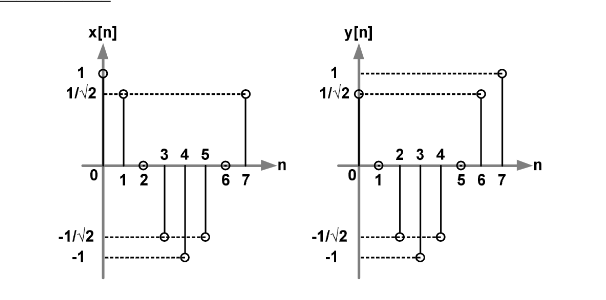
\includegraphics[width=1\columnwidth]{2022/BM/15/figs/question_BM_15.png}
    \caption{Question Figure}
    \label{fig:question_fig}
\end{figure}\hfill{(GATE BM 2022)}\\
\solution
\iffalse
\let\negmedspace\undefined
\let\negthickspace\undefined
\documentclass[journal,12pt,twocolumn]{IEEEtran}
\usepackage{cite}
\usepackage{amsmath,amssymb,amsfonts,amsthm}
\usepackage{algorithmic}
\usepackage{graphicx}
\usepackage{textcomp}
\usepackage{xcolor}
\usepackage{txfonts}
\usepackage{listings}
\usepackage{enumitem}
\usepackage{mathtools}
\usepackage{float}
\usepackage{gensymb}
\usepackage{comment}
\usepackage[breaklinks=true]{hyperref}
\usepackage{tkz-euclide} 
\usepackage{listings}
\usepackage{gvv}                                        
\def\inputGnumericTable{}                                 
\usepackage[latin1]{inputenc}                                
\usepackage{color}                                            
\usepackage{array}          
\usetikzlibrary{positioning, arrows.meta}
\usepackage{longtable}                                       
\usepackage{calc}                                             
\usepackage{multirow}                                         
\usepackage{hhline}                                           
\usepackage{ifthen}                                           
\usepackage{lscape}
\usepackage{amsmath}
\newtheorem{theorem}{Theorem}[section]
\newtheorem{problem}{Problem}
\newtheorem{proposition}{Proposition}[section]
\newtheorem{lemma}{Lemma}[section]
\newtheorem{corollary}[theorem]{Corollary}
\newtheorem{example}{Example}[section]
\newtheorem{definition}[problem]{Definition}
\newcommand{\BEQA}{\begin{eqnarray}}
\newcommand{\EEQA}{\end{eqnarray}}
\newcommand{\define}{\stackrel{\triangle}{=}}
\theoremstyle{remark}
\newtheorem{rem}{Remark}
\begin{document}

\bibliographystyle{IEEEtran}
\title{GATE-BM-Q15}
\author{EE23BTECH11015 - DHANUSH V NAYAK$^{*}$% <-this % stops a space
}
\maketitle
\newpage
\bigskip
\renewcommand{\thefigure}{\arabic{figure}}
\renewcommand{\thetable}{\theenumi}
\textbf{Question:} Discrete signals $x\brak{n}$ and $y\brak{n}$ are shown below. The cross-correlation $r_{xy}\brak{0}$ is:
\begin{figure}[H]
    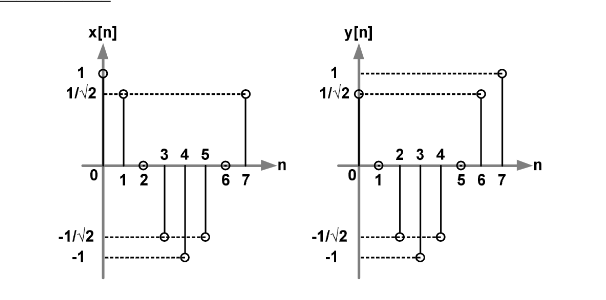
\includegraphics[width=1\columnwidth]{2022/BM/15/figs/question_BM_15.png}
    \caption{Question Figure}
    \label{fig:question_fig}
\end{figure}\hfill{(GATE BM 2022)}\\
\solution
\fi
\begin{table}[H]
\centering
\renewcommand\thetable{1}
\setlength{\extrarowheight}{9pt}
\resizebox{0.5\textwidth}{!}{
\begin{tabular}{|c|c|c|}
\hline
\textbf{Parameter} & \textbf{Description} & \textbf{Value} \\ \hline
$x\brak{n}$ & First Sequence & $x(n) = 
\begin{cases}
    0 & ; n < 0 \\
    \brak{1,\frac{1}{\sqrt{2}} , 0 ,-\frac{1}{\sqrt{2}},-1,-\frac{1}{\sqrt{2}},0,\frac{1}{\sqrt{2}}} & ; 0 \leq n \leq 7 \\
    0 & ; n > 7 \\
\end{cases}$   \\ \hline
$y\brak{n}$ &Second Sequence &$y(n) = 
\begin{cases}
    0 & ; n < 0 \\
    \brak{\frac{1}{\sqrt{2}} , 0 ,-\frac{1}{\sqrt{2}},-1,-\frac{1}{\sqrt{2}},0,\frac{1}{\sqrt{2}},1} & ; 0 \leq n \leq 7 \\
    0 & ; n > 7 \\
\end{cases}$  \\ \hline
$r_{xy}\brak{k}$& Cross-correlation & $\sum_{m=-\infty}^{\infty} x\brak{m}y\brak{m-k}$ \\ \hline 
\end{tabular}}
\caption{Parameter Table}
\label{tab:gate_bm_Q15}
\end{table}

It can be seen that :
\begin{align}
    y\brak{n} = x\brak{n+1}\label{eq:gate_bm_q15.1}
\end{align}
From \tabref{tab:gate_bm_Q15} :
\begin{align}
    r_{xy}\brak{k} &= \sum_{m=-\infty}^{\infty} x\brak{m}y\brak{m-k}\\
                &= x\brak{k} * y\brak{-k}
\end{align}
From \eqref{eq:gate_bm_q15.1}:
\begin{align}
    r_{xy}\brak{k} &= x\brak{k+1} * x\brak{-k}\\
                &= \sum_{n=-\infty}^{\infty} x\brak{n+1}x\brak{n+k} 
\end{align}
By definition of x\brak{n} from \tabref{tab:gate_bm_Q15}:
\begin{align}
     r_{xy}\brak{k} &= \sum_{n=0}^{6} x\brak{n+1}x\brak{n+k} \\
     r_{xy}\brak{0} &= \sum_{n=0}^{6} x\brak{n+1}x\brak{n} 
\end{align}
Using values from \figref{fig:question_fig}:
\begin{align}
    r_{xy}\brak{0} &= 2\sqrt{2}
\end{align}
\begin{figure}[H]
    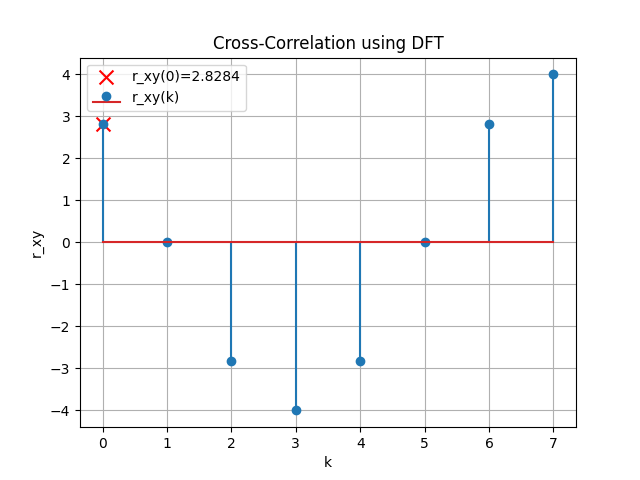
\includegraphics[width=1\columnwidth]{2022/BM/15/figs/cross-corelation.png}
    \caption{Verification of result by DFT}
    \label{fig:cross-corelation}
\end{figure}

%\end{document}


\pagebreak

\end{enumerate}

\section{2021}
\begin{enumerate}[label=\thechapter.\arabic*,ref=\thechapter.\theenumi]
\item 
\solution
\input{}
\pagebreak
\end{enumerate}

\chapter{Sampling}
\section{2022}
\begin{enumerate}[label=\thechapter.\arabic*,ref=\thechapter.\theenumi]

\item 
\newpage

\end{enumerate}

\section{2021}
\begin{enumerate}[label=\thechapter.\arabic*,ref=\thechapter.\theenumi]
\item An analog signal is sampled at 100 MHz to generate 1024 samples. Only
these samples are used to evaluate 1024-point FFT. The separation between
adjacent frequency points ($\Delta$F) in FFT is \rule{1cm}{0.5mm} kHz.\\
\hfill (GATE BM 2021)\\
\solution
\iffalse
\documentclass[journal,12pt,twocolumn]{IEEEtran}
\usepackage{amsmath,amssymb,amsfonts,amsthm}
\usepackage{txfonts}
\usepackage{tkz-euclide}
\usepackage{listings}
\usepackage{gvv}
\usepackage[latin1]{inputenc}
\usepackage{adjustbox}
\usepackage{array}
\usepackage{tabularx}
\usepackage{pgf}
\usepackage{lmodern}
\usepackage{circuitikz}
\usepackage{tikz}
\usepackage{graphicx}
\usepackage[english]{babel}

\begin{document}
\bibliographystyle{IEEEtran}

\vspace{3cm}

\title{}
\author{EE23BTECH11047 - Deepakreddy P
}
\maketitle
\newpage
\bigskip

\noindent \textbf{32} \quad An analog signal is sampled at 100 MHz to generate 1024 samples. Only
these samples are used to evaluate 1024-point FFT. The separation between
adjacent frequency points ($\Delta$F) in FFT is \rule{1cm}{0.5mm} kHz.\\
\hfill (GATE BM 2021)\\
\solution
\fi

\begin{center}
    \begin{table}[ht]
        \setlength{\arrayrulewidth}{0.3mm}
\setlength{\tabcolsep}{12pt}
\renewcommand{\arraystretch}{1.3}


\begin{center}
\caption{Input Parameters}
\begin{tabular}{ |p{1.7cm}|p{1.7cm}|p{1.7cm}|  }

\hline
 {Symbol}&{Description} & {value}\\
\hline
$f_s$ & Sampling frequency & 100 MHz\\
\hline
$N$ & No of samples  & 1024\\
\hline

\end{tabular}
\end{center}

    \end{table}
\end{center}

\begin{align}
    \Delta F &= \frac{f_s}{N}\\
    \Delta F &= \frac{100}{1024} MHz\\
    \Delta F &= \frac{10^5}{1024} kHz\\
    \Delta F &= 97.66kHz
\end{align}


\begin{figure}[ht]
   \centering
   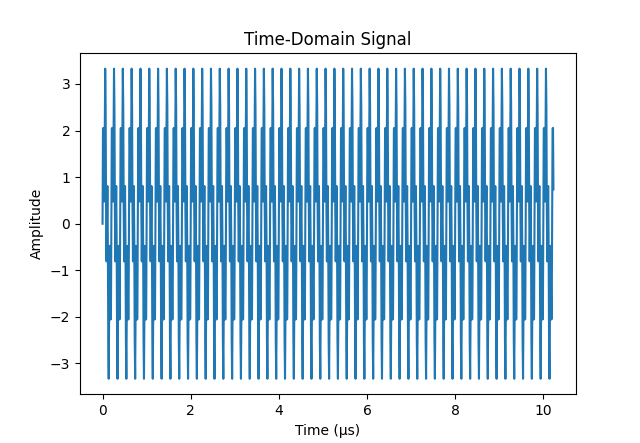
\includegraphics[width=1.1\columnwidth]{2021/BM/32/figs/fig1.png}
   \caption{Time Domain Signal}
\end{figure}

\begin{figure}[ht]
   \centering
   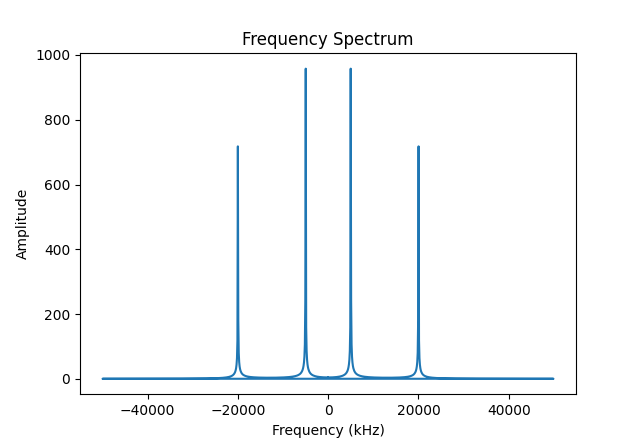
\includegraphics[width=1.1\columnwidth]{2021/BM/32/figs/fig2.png}
   \caption{Frequency Spectrum}
\end{figure}






%\end{document}


\newpage

\item Consider a real-valued base-band signal $x(t)$, band limited to $10kHz$. The Nyquist rate for the signal \\\\
$y(t) = x(t)x(1+\dfrac{t}{2})$ is\\

\begin{enumerate}
\item[(A)] $15kHz$
\item[(B)] $30kHz$
\item[(C)] $60kHz$
\item[(D)] $20kHz$
\end{enumerate}
\hfill{(GATE EC 2021)}\\
\solution
\iffalse
\documentclass[journal,12pt,twocolumn]{IEEEtran}
\usepackage{cite}
\usepackage{amsmath,amssymb,amsfonts,amsthm}
\usepackage{algorithmic}
\usepackage{graphicx}
\usepackage{textcomp}
\usepackage{xcolor}
\usepackage{txfonts}
\usepackage{listings}
\usepackage{enumitem}
\usepackage{mathtools}
\usepackage{gensymb}
\usepackage{comment}
\usepackage[breaklinks=true]{hyperref}
\usepackage{tkz-euclide}
\usepackage{listings}
\usepackage{gvv}
\def\inputGnumericTable{}
\usepackage[latin1]{inputenc}
\usepackage{color}
\usepackage{array}
\usepackage{longtable}
\usepackage{calc}
\usepackage{multirow}
\usepackage{hhline}
\usepackage{ifthen}
\usepackage{lscape}
\usepackage{circuitikz}
\usepackage{geometry}

\newtheorem{theorem}{Theorem}[section]
\newtheorem{problem}{Problem}
\newtheorem{proposition}{Proposition}[section]
\newtheorem{lemma}{Lemma}[section]
\newtheorem{corollary}[theorem]{Corollary}
\newtheorem{example}{Example}[section]
\newtheorem{definition}[problem]{Definition}
\newcommand{\BEQA}{\begin{eqnarray}}
\newcommand{\EEQA}{\end{eqnarray}}
\newcommand{\define}{\stackrel{\triangle}{=}}
\theoremstyle{remark}
\newtheorem{rem}{Remark}

\begin{document}

\bibliographystyle{IEEEtran}
\vspace{3cm}

\title{Gate 2021- EC}
\author{EE23BTECH11058 - Sindam Ananya$^{*}$% <-this % stops a space
}
\maketitle
\newpage
\bigskip

\renewcommand{\thefigure}{\theenumi}
\renewcommand{\thetable}{\theenumi}

\vspace{3cm}
\textbf{Question 4:} 
Consider a real-valued base-band signal $x(t)$, band limited to $10kHz$. The Nyquist rate for the signal \\\\
$y(t) = x(t)x(1+\dfrac{t}{2})$ is\\

\begin{enumerate}
\item[(A)] $15kHz$
\item[(B)] $30kHz$
\item[(C)] $60kHz$
\item[(D)] $20kHz$
\end{enumerate}
\hfill{(GATE EC 2021)}\\
\solution
\fi
\begin{table}[h!]
\centering
\begin{tabular}{|c|c|c|}
\hline
\textbf{Parameter} & \textbf{Value} & \textbf{Description}\\
\hline
$x(t)$ & & base-band signal\\
\hline
$f$ & $10kHz$ & Maximum frequency of $X(f)$\\
\hline
$y(t)$ & $x(t)x(1+\dfrac{t}{2})$ & new signal\\
\hline
$f_{max}$ & & Maximum frequency of $Y(f)$\\
\hline
\end{tabular}

\caption{Input Parameters}
\label{tab:gate2021ec4table}
\end{table}
\begin{align}
x(t) &\xleftrightarrow{\mathcal{F}} X(j\omega)\\
x(at) &\xleftrightarrow{\mathcal{F}} \frac{1}{a}X(j\omega)\\
x(t-t_o) &\xleftrightarrow{\mathcal{F}} e^{-j\omega t_o}X(j\omega)\\
x(1+\frac{t}{2}) &\xleftrightarrow{\mathcal{F}} 2e^{j\omega}X(j2\omega)\\
y(t) &= x(t)x(1+\frac{t}{2})\\
x_1(t)x_2(t) &\xleftrightarrow{\mathcal{F}} X_1(f) * X_2(f)\\
Y(f) &= X(f) * 2e^{j2\pi f}X(2f)
\end{align}
\begin{figure}[h!]
    \centering
    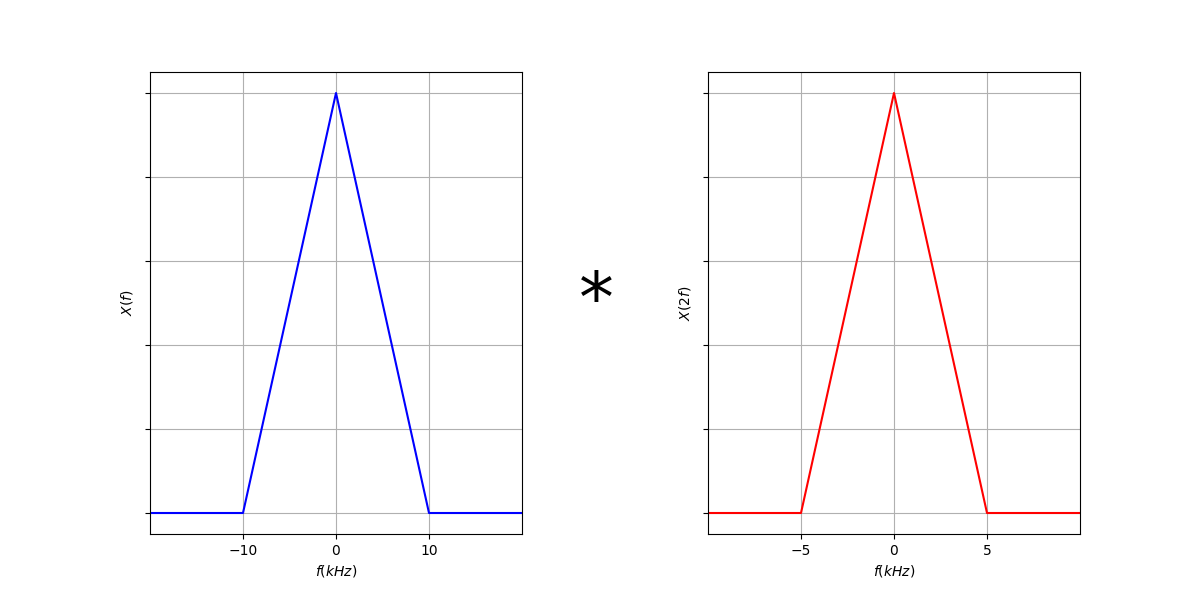
\includegraphics[width=\columnwidth]{2021/EC/4/figs/plot1.png}
    \caption{Plot of $X(f)$ and $X(2f)$}
    \label{fig:gate2021ec4fig1}
\end{figure}
\begin{figure}[h!]
    \centering
    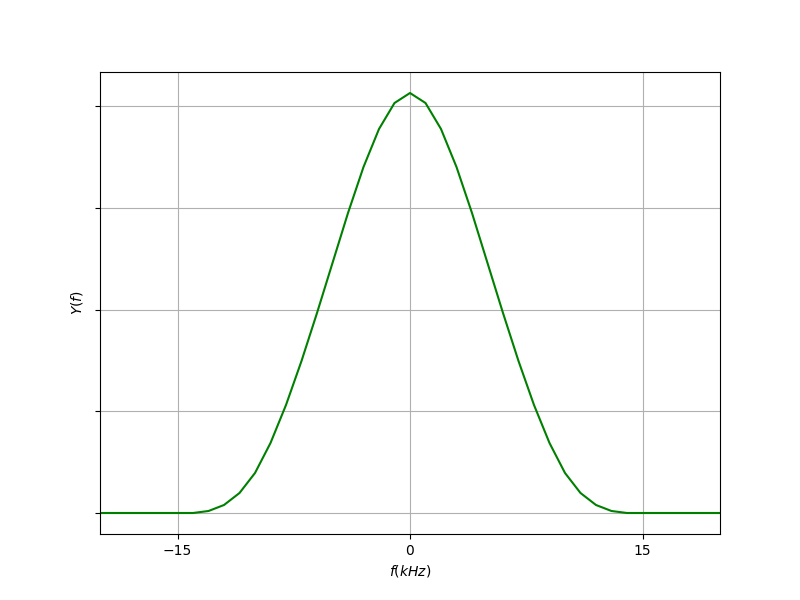
\includegraphics[width=\columnwidth]{2021/EC/4/figs/plot2.png}
    \caption{Plot of $Y(f)$}
    \label{fig:gate2021ec4fig2}
\end{figure}
Nyquist rate is $2f_{max} = 2(15kHz)$ which is $30kHz$
%\end{document}


\newpage

\end{enumerate}

\chapter{Contour Integration}
\section{2022}
\begin{enumerate}[label=\thechapter.\arabic*,ref=\thechapter.\theenumi]
\item In the complex $z$-domain, the value of integral $\oint_{C}\frac{z^3-9}{3z-i}\;dz$ is   \\
\begin{enumerate}[label=(\alph*)]
    \item $\frac{2\pi}{81}-6i\pi$ 
    \item $\frac{2\pi}{81}+6i\pi$ 
    \item $-\frac{2\pi}{81}+6i\pi$ 
    \item $-\frac{2\pi}{81}-6i\pi$ 
\end{enumerate} \hfill(GATE 2022 BM)    \\
\solution
% \iffalse
\let\negmedspace\undefined
\let\negthickspace\undefined
\documentclass[journal,12pt,twocolumn]{IEEEtran}
\usepackage{cite}
\usepackage{amsmath,amssymb,amsfonts,amsthm}
\usepackage{algorithmic}
\usepackage{graphicx}
\usepackage{textcomp}
\usepackage{xcolor}
\usepackage{txfonts}
\usepackage{listings}
\usepackage{enumitem}
\usepackage{mathtools}
\usepackage{gensymb}
\usepackage{comment}
\usepackage[breaklinks=true]{hyperref}
\usepackage{tkz-euclide} 
\usepackage{listings}
\usepackage{gvv}                                        
\def\inputGnumericTable{}                                 
\usepackage[latin1]{inputenc}                                
\usepackage{color}                                            
\usepackage{array}                                            
\usepackage{longtable}                                       
\usepackage{calc}                                             
\usepackage{multirow}                                         
\usepackage{hhline}                                           
\usepackage{ifthen}                                           
\usepackage{lscape}

\newtheorem{theorem}{Theorem}[section]
\newtheorem{problem}{Problem}
\newtheorem{proposition}{Proposition}[section]
\newtheorem{lemma}{Lemma}[section]
\newtheorem{corollary}[theorem]{Corollary}
\newtheorem{example}{Example}[section]
\newtheorem{definition}[problem]{Definition}
\newcommand{\BEQA}{\begin{eqnarray}}
\newcommand{\EEQA}{\end{eqnarray}}
\newcommand{\define}{\stackrel{\triangle}{=}}
\theoremstyle{remark}
\newtheorem{rem}{Remark}
\begin{document}
\parindent 0px
\bibliographystyle{IEEEtran}
\title{GATE: BM - 36.2022}
\author{EE22BTECH11219 - Rada Sai Sujan$^{}$% <-this % stops a space
}
\maketitle
\newpage
\bigskip
\section*{Question}
In the complex $z$-domain, the value of integral $\oint_{C}\frac{z^3-9}{3z-i}\;dz$ is   \\
\begin{enumerate}[label=(\alph*)]
    \item $\frac{2\pi}{81}-6i\pi$ 
    \item $\frac{2\pi}{81}+6i\pi$ 
    \item $-\frac{2\pi}{81}+6i\pi$ 
    \item $-\frac{2\pi}{81}-6i\pi$ 
\end{enumerate} \hfill(GATE 2022 BM)    \\
\solution

Simplyfying the Contour Integral to the standard form we get,
\begin{align}
    \oint_{C}\frac{z^3-9}{3z-i}\;dz &= \frac{1}{3}\oint_{C}\frac{z^3-9}{z-\frac{i}{3}}\;dz
\end{align}
From Cauchy's residue theorem,
\begin{align}
    \oint_{C}f(z)\;dz &= 2\pi i\sum R_j \label{equation:bm.2022.36Q.2}
\end{align}
We can observe a non-repeated pole at $z=\frac{i}{3}$ and thus $a=\frac{i}{3}$,
\begin{align}
    R &= \lim\limits_{z\to a}\brak{z-a}f\brak{z}    \\
    \implies R &= \frac{1}{3}\lim\limits_{z\to \frac{i}{3}}\brak{z-\frac{i}{3}}\frac{z^3-9}{z-\frac{i}{3}}  \\
    &= \frac{-i}{81}-3  \label{equation:bm.2022.36Q.5}
\end{align}
Therefore, from \eqref{equation:bm.2022.36Q.2} and \eqref{equation:bm.2022.36Q.5}
\begin{align}
    \oint_{C}\frac{z^3-9}{3z-i}\;dz &= \frac{2\pi}{81}-6i\pi
\end{align}
\end{document}

\newpage
\item Consider the function
\begin{align*}
f\brak{z} = \frac{1}{\brak{z+1}\brak{z+2}\brak{z+3}}
\end{align*}
The residue of $f\brak{z}$ at $z=-1$, is \rule{1cm}{0.15mm}
\hfill(GATE 2022 IN) \\
\solution
\iffalse
\let\negmedspace\undefined
\let\negthickspace\undefined
\documentclass[journal,12pt,twocolumn]{IEEEtran}
\usepackage{cite}
\usepackage{amsmath,amssymb,amsfonts,amsthm}
\usepackage{algorithmic}
\usepackage{graphicx}
\usepackage{textcomp}
\usepackage{xcolor}
\usepackage{txfonts}
\usepackage{listings}
\usepackage{enumitem}
\usepackage{mathtools}
\usepackage{gensymb}
\usepackage{comment}
\usepackage[breaklinks=true]{hyperref}
\usepackage{tkz-euclide}
\usepackage{listings}
\usepackage{gvv}
\def\inputGnumericTable{}
\usepackage[latin1]{inputenc}
\usepackage{color}
\usepackage{array}
\usepackage{longtable}
\usepackage{calc}
\usepackage{multirow}
\usepackage{hhline}
\usepackage{ifthen}
\usepackage{lscape}

\newtheorem{theorem}{Theorem}[section]
\newtheorem{problem}{Problem}
\newtheorem{proposition}{Proposition}[section]
\newtheorem{lemma}{Lemma}[section]
\newtheorem{corollary}[theorem]{Corollary}
\newtheorem{example}{Example}[section]
\newtheorem{definition}[problem]{Definition}
\newcommand{\BEQA}{\begin{eqnarray}}
\newcommand{\EEQA}{\end{eqnarray}}
\newcommand{\define}{\stackrel{\triangle}{=}}
\theoremstyle{remark}
\newtheorem{rem}{Remark}
\begin{document}

\bibliographystyle{IEEEtran}
\vspace{3cm}

\title{GATE 2022 IN 61}
\author{EE23BTECH11007 - Aneesh Kadiyala$^{*}$% <-this % stops a space
}
\maketitle
\newpage
\bigskip

\renewcommand{\thefigure}{\theenumi}
\renewcommand{\thetable}{\theenumi}

\vspace{3cm}
\textbf{Question:} Consider the function
\begin{align*}
f\brak{z} = \frac{1}{\brak{z+1}\brak{z+2}\brak{z+3}}
\end{align*}
The residue of $f\brak{z}$ at $z=-1$, is \rule{1cm}{0.15mm}

\hfill(GATE 2022 IN 61)
\\
\solution
\\
\fi
Residue of a function $f\brak{z}$ at a simple pole $c$ is
\begin{align}
\text{Res}\brak{f, c} &= \lim_{z \to c}\brak{z - c}f\brak{z} \\
\implies \text{Res}\brak{f,-1} &= \lim_{z \to -1}\frac{z + 1}{\brak{z+1}\brak{z+2}\brak{z+3}} \\
&= \frac{1}{2}
\end{align}
$\therefore$ residue of $f\brak{z}$ at $z = -1$ is $\frac{1}{2}$.
\newpage
\end{enumerate}

\section{2021}
\begin{enumerate}[label=\thechapter.\arabic*,ref=\thechapter.\theenumi]
\item 
\solution
\input{}
\pagebreak
\end{enumerate}

\chapter{Laplace Transform}
\section{2022}
 \begin{enumerate}[label=\thechapter.\arabic*,ref=\thechapter.\theenumi]

\item Consider the differential equation $\frac{d^2y}{dx^2}-2\frac{dy}{dx}+y=0$. The boundary conditions are $y=0$ and $\frac{dy}{dx}=1$ at $x=0$. Then the value of $y$ at $x=\frac{1}{2}$ \hfill (GATE AE 2022)\\
\solution
\iffalse
\let\negmedspace\undefined
\let\negthickspace\undefined
\documentclass[journal,12pt,twocolumn]{IEEEtran}
\usepackage{cite}
\usepackage{amsmath,amssymb,amsfonts,amsthm}
\usepackage{algorithmic}
\usepackage{graphicx}
\usepackage{textcomp}
\usepackage{xcolor}
\usepackage{txfonts}
\usepackage{listings}
\usepackage{enumitem}
\usepackage{mathtools}
\usepackage{gensymb}
\usepackage{comment}
\usepackage[breaklinks=true]{hyperref}
\usepackage{tkz-euclide} 
\usepackage{listings}
\usepackage{gvv}                                        
\def\inputGnumericTable{}                                 
\usepackage[latin1]{inputenc}                                
\usepackage{color}                                            
\usepackage{array}                                            
\usepackage{longtable}                                       
\usepackage{calc}                                             
\usepackage{multirow}                                         
\usepackage{hhline}                                           
\usepackage{ifthen}                                           
\usepackage{lscape}
\newtheorem{theorem}{Theorem}[section]
\newtheorem{problem}{Problem}
\newtheorem{proposition}{Proposition}[section]
\newtheorem{lemma}{Lemma}[section]
\newtheorem{corollary}[theorem]{Corollary}
\newtheorem{example}{Example}[section]
\newtheorem{definition}[problem]{Definition}
\newcommand{\BEQA}{\begin{eqnarray}}
\newcommand{\EEQA}{\end{eqnarray}}
\newcommand{\define}{\stackrel{\triangle}{=}}
\theoremstyle{remark}
\newtheorem{rem}{Remark}
\begin{document}

\bibliographystyle{IEEEtran}
\vspace{3cm}

\title{GATE: AE - 37.2022}
\author{EE23BTECH11224 - Sri Krishna Prabhas Yadla$^{*}$% <-this % stops a space
}
\maketitle
\newpage
\bigskip

\renewcommand{\thefigure}{\arabic{figure}}
\renewcommand{\thetable}{\arabic{table}}


\vspace{3cm}
\textbf{Question:} Consider the differential equation $\frac{d^2y}{dx^2}-2\frac{dy}{dx}+y=0$. The boundary conditions are $y=0$ and $\frac{dy}{dx}=1$ at $x=0$. Then the value of $y$ at $x=\frac{1}{2}$ \hfill (GATE AE 2022)\\
\solution
\fi
\begin{table}[htbp]
	\centering
	\def\arraystretch{1.5}
	\begin{tabular}{|c|c|c|}
\hline
\textbf{Parameters} & \textbf{Values} & \textbf{Description} \\
\hline
$y(0)$ & 0 & $y$ at $x=0$\\
\hline
$y'(0)$& 1 &$\frac{dy}{dx}$ at $x=0$ \\
\hline
\end{tabular}

	\caption{Parameters}
	\label{tab:parameters}
\end{table}
\begin{align}
\label{L(y'')}\frac{d^2y}{dx^2} &\system{L} s^2Y(s)-sy(0)-y'(0)\\
\label{L(y')}\frac{dy}{dx} &\system{L} sY(s)-y(0)
\end{align}
Applying Laplace Transform, using \eqref{L(y'')} and \eqref{L(y')},
\begin{align}
s^2Y(s)-sy(0)-y'(0) - 2(sY(s)-y(0)) + Y(s) = 0
\end{align}
From \tabref{tab:parameters},
\begin{align}
(s^2-2s+1)Y(s)-1 &= 0 \\
Y(s) &= \frac{1}{(s-1)^2}\\
\label{L(t^n)}t^n &\system{L} \frac{n!}{s^{n+1}}\\
	\label{complex_shift}e^{at} x(t) &\system{L} X(s-a)
\end{align}
Taking Inverse Laplace Transform for $Y(s)$, using \eqref{L(t^n)} and \eqref{complex_shift},
\begin{align}
y(x) &= xe^x \\
\implies y\brak{\frac{1}{2}} &= \frac{\sqrt{e}}{2}
\end{align}
\begin{figure}[htbp]
	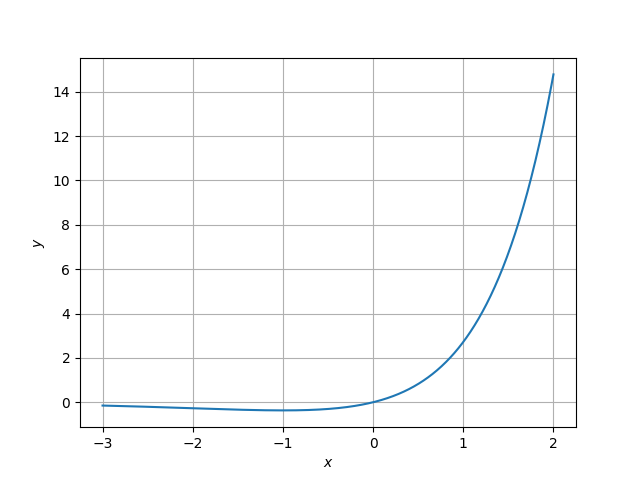
\includegraphics[width=\columnwidth]{2022/AE/37/figs/plot.png}
	\caption{Plot of $y(x)$}
	\label{fig:plot}
\end{figure}

\pagebreak

\item  A process described by the transfer function
\begin{align}
    G_p(s) = \frac{\brak{10s+1}}{\brak{5s+1}} \nonumber
\end{align}
is forced by a unit step input at time $t = 0$. The output value immediately after the unit step input (at $t = 0^+$) is ? \hfill(Gate 2022 CH 34)\\
\solution
\iffalse
\documentclass[journal,12pt,twocolumn]{IEEEtran}
\usepackage{cite}
\usepackage{amsmath,amssymb,amsfonts,amsthm}
\usepackage{algorithmic}
\usepackage{graphicx}
\usepackage{textcomp}
\usepackage{xcolor}
\usepackage{txfonts}
\usepackage{listings}
\usepackage{enumitem}
\usepackage{mathtools}
\usepackage{gensymb}
\usepackage{comment}
\usepackage[breaklinks=true]{hyperref}
\usepackage{tkz-euclide}
\usepackage{listings}
\usepackage{gvv}
\def\inputGnumericTable{}
\usepackage[latin1]{inputenc}
\usepackage{color}
\usepackage{array}
\usepackage{longtable}
\usepackage{calc}
\usepackage{multirow}
\usepackage{hhline}
\usepackage{ifthen}
\usepackage{lscape}
\usepackage{caption}

\newtheorem{theorem}{Theorem}[section]
\newtheorem{problem}{Problem}
\newtheorem{proposition}{Proposition}[section]
\newtheorem{lemma}{Lemma}[section]
\newtheorem{corollary}[theorem]{Corollary}
\newtheorem{example}{Example}[section]
\newtheorem{definition}[problem]{Definition}
\newcommand{\BEQA}{\begin{eqnarray}}
\newcommand{\EEQA}{\end{eqnarray}}
\newcommand{\define}{\stackrel{\triangle}{=}}
\theoremstyle{remark}
\newtheorem{rem}{Remark}
\begin{document}

\bibliographystyle{IEEEtran}
\vspace{3cm}

\title{GATE: CH - 34.2022}
\author{EE23BTECH11010 - Venkatesh D Bandawar $^{*}$% <-this % stops a space
}
\maketitle
% \newpage
\bigskip

% \renewcommand{\thefigure}{\theenumi}
% \renewcommand{\thetable}{\theenumi}

\textbf{Question:} A process described by the transfer function
\begin{align}
    G_p(s) = \frac{\brak{10s+1}}{\brak{5s+1}} \nonumber
\end{align}
is forced by a unit step input at time $t = 0$. The output value immediately after the unit step input (at $t = 0^+$) is ? \hfill(Gate 2022 CH 34)\\
\solution
\fi
\begin{table}[!h] 
\centering
\begin{tabular}{|c|c|}
\hline
     \textbf{Parameters}&\textbf{Description}  \\
     \hline
     $X(s)$ & Laplace transform of $x(t)$ \\
     \hline
     $Y(s)$ & Laplace transform of $y(t)$ \\
     \hline
     $G_p(s) = \frac{Y(s)}{X(s)}$ & Transfer function\\
     \hline
     $x(t) = u(t)$ & unit step function\\
     \hline
\end{tabular}

\caption{Given parameters}
\label{given parameters list.gate.2022.ch.34}
\end{table}
\begin{align}
    G_p(s) = \frac{Y(s)}{X(s)} &= \frac{\brak{10s+1}}{\brak{5s+1}}\\
    u(t) \system{\mathcal{L}} \frac{1}{s} \label{laplace transform of unit function 2022.ch.34}
\end{align}
From equation \eqref{laplace transform of unit function 2022.ch.34}:
\begin{align}
    Y(s) &= \frac{\brak{10s+1}}{s\brak{5s+1}}\\
    &= \frac{1}{s} + \frac{5}{5s+1}
\end{align}
Taking inverse laplace transformation, 
\begin{align}
    \frac{1}{s} &\mathrel{\substack{\mathcal{L}^{-1}\\\longleftrightarrow}} u(t)\\
    \frac{1}{s-c} &\mathrel{\substack{\mathcal{L}^{-1}\\\longleftrightarrow}} e^{ct} u(t)
\end{align}
\begin{align}
    y(t) &= \brak{1 + e^{\frac{-t}{5}}}u(t)\\
    y(0^+) &= 2
\end{align}

\begin{figure}[!h] 
    \centering
    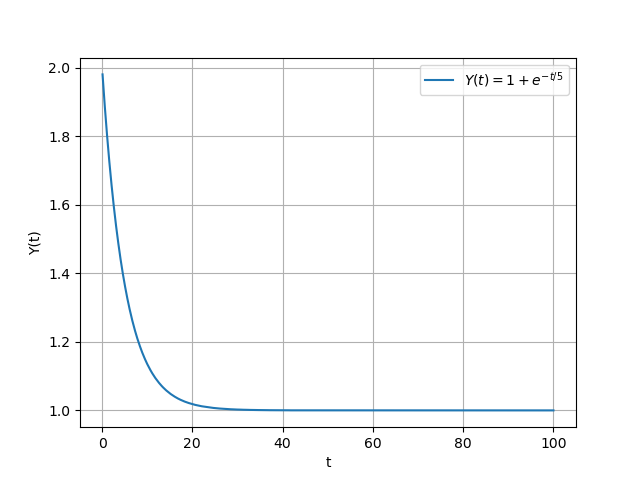
\includegraphics[width=\columnwidth]{2022/CH/34/figs/Graph_of_y(t).png}
    \caption{Graph of y(t)}
    \label{fig:Graph1_gate_CE_30}
    \end{figure}


\pagebreak
\item The transfer function of a real system $H(S)$ is given as:
\begin{align}
    H(s) = \frac{As + B}{s^2 + Cs + D}\nonumber
\end{align}
where $A, B, C$ and $D$ are positive constants. This system cannot operate as
\begin{enumerate}[label={(\Alph*)}]
    \item Low pass filter
    \item High pass filter
    \item Band pass filter
    \item An Integrator
\end{enumerate}\hfill(GATE EE 11 2022)

\solution
 \iffalse
\let\negmedspace\undefined
\let\negthickspace\undefined
\documentclass[journal,12pt,twocolumn]{IEEEtran}
\usepackage{cite}
\usepackage{amsmath,amssymb,amsfonts,amsthm}
\usepackage{algorithmic}
\usepackage{graphicx}
\usepackage{textcomp}
\usepackage{xcolor}
\usepackage{txfonts}
\usepackage{listings}
\usepackage{enumitem}
\usepackage{mathtools}
\usepackage{gensymb}
\usepackage{comment}
\usepackage[breaklinks=true]{hyperref}
\usepackage{tkz-euclide} 
\usepackage{listings}
\usepackage{gvv} 
\usepackage{caption}
\def\inputGnumericTable{}                   

%\usepackage[latin1]{inputenc}                                
\usepackage{color}                                            
\usepackage{array}                                            
\usepackage{longtable}                                       
\usepackage{calc}                                             
\usepackage{multirow}                                         
\usepackage{hhline}                                           
\usepackage{ifthen}                                           
\usepackage{lscape}
\usepackage{tikz}
\newtheorem{theorem}{Theorem}[section]
\newtheorem{problem}{Problem}
\newtheorem{proposition}{Proposition}[section]
\newtheorem{lemma}{Lemma}[section]
\newtheorem{corollary}[theorem]{Corollary}
\newtheorem{example}{Example}[section]
\newtheorem{definition}[problem]{Definition}
\newcommand{\BEQA}{\begin{eqnarray}}
\newcommand{\EEQA}{\end{eqnarray}}
\newcommand{\define}{\stackrel{\triangle}{=}}
\theoremstyle{remark}
\newtheorem{rem}{Remark}

\begin{document}

\bibliographystyle{IEEEtran}
\vspace{3cm}

\title{GATE: EE - 11.2022}
\author{EE23BTECH11013 - Avyaaz$^{*}$% <-this % stops a space 
}
\maketitle
\newpage
\bigskip

\renewcommand{\thefigure}{\arabic{figure}}
\renewcommand{\thetable}{\arabic{table}}

\large\textbf{\textsl{Question:}}
The transfer function of a real system $H(S)$ is given as:
\begin{align}
    H(s) = \frac{As + B}{s^2 + Cs + D}\nonumber
\end{align}
where $A, B, C$ and $D$ are positive constants. This system cannot operate as
\begin{enumerate}[label={(\Alph*)}]
    \item Low pass filter
    \item High pass filter
    \item Band pass filter
    \item An Integrator
\end{enumerate}\hfill(GATE EE 11 2022) \\
\solution
\fi
The transfer function $H(s)$ is given by: 
\begin{align}
    H(s) = \frac{As + B}{s^2 + Cs + D}\label{eq:given.EE.11.2022}
\end{align}
Put $s = j\omega$ in \eqref{eq:given.EE.11.2022}:
\begin{align}
    H(j\omega) = \frac{A(j\omega) + B}{(j\omega)^2 + C(j\omega) + D} \\
    |H(j\omega)| = \frac{\sqrt{(A\omega)^2 + B^2}}{\sqrt{(D - \omega^2)^2 + (\omega C)^2}}\label{eq:magnitude.EE.11.2022}
\end{align}


\begin{table}[htbp]
\setlength{\extrarowheight}{4pt}
\setlength{\tabcolsep}{3pt}
\centering
\begin{tabular}{|c|c|}
\hline
\textbf{Parameter} & \textbf{Description}\\
\hline 
Low Pass Filter & The gain should be finite at low frequency  \\
\hline
High Pass Filter &The gain should be finite at high frequency \\
\hline
Band Pass Filter& Finite gain over frequency band \\
\hline
Integrator & Transfer function should have at least\\& one pole at origin \\
\hline
\end{tabular}

\caption{Conditions}
\label{tab:inputs.EE.11.2022}
\end{table}
% \item \noindent From \tabref{tab:inputs.EE.11.2022} and equation \eqref{eq:magnitude.EE.11.2022}:
\begin{enumerate}[label={\alph*)}]
    \item Low Pass Filter:
    
  At low frequency $(\omega = 0 )$:
 \begin{align}
     |H(\omega = 0)| = \frac{B}{D}\label{eq:lowpass.EE.11.2022}
 \end{align}
$\therefore$ H(s) can operate as Low pass filter.

\item High Pass Filter:

% From \tabref{tab:inputs.EE.11.2022} and equation \eqref{eq:magnitude.EE.11.2022}:

At high frequency $(\omega = \infty )$:
 \begin{align}
     |H(\omega = \infty)| = 0 \label{eq:highpass.EE.11.2022}
 \end{align}
 % From \tabref{tab:inputs.EE.11.2022}:
 
$\therefore$ $H(s)$ cannot operate as High pass filter.
\item Band Pass Filter:

 Assuming B is a very less positive valued constant as compared to others:
\begin{align}
        |H(j\omega)| = \frac{(A\omega)}{\sqrt{(D - \omega^2)^2 + (\omega C)^2}}\\
   \implies      |H(\omega = 0)| = 0 \text{ and }  |H(\omega = \infty)| = 0 \label{eq:bandpass.EE.11.2022}
\end{align}

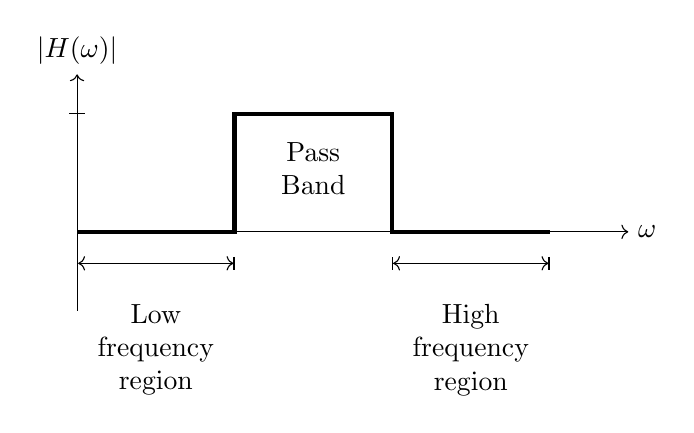
\begin{tikzpicture}
  
    \draw[->] (0,0) -- (7,0) node[right] {$\omega$};
   
    \draw[->] (0,-1) -- (0,2) node[above] {$|H(\omega)|$};
  
    \draw[line width=1.5pt]  (0,0) -- (2,0) -- (2,1.5) -- (4,1.5) -- (4,0) --(6,0);
    \draw[-]{(0,1.5)};
      \draw (-0.1,1.5) -- (0.1,1.5);
         \draw[|<->|]{(0,-0.4) -- (2,-0.4)};
    \node[align=center] at (1,-1.5) {Low \\frequency\\ region};
         \draw[| <-> |]{(4,-0.4) -- (6,-0.4)};
    \node[align=center] at (5,-1.5) {High \\frequency\\ region};
    \node[align=center] at (3,0.8) {Pass\\Band};

\end{tikzpicture}
$\because$ $H(s)$ passes frequency between low and high frequencies.

$\therefore$ $H(s)$ can operate as a band pass filter.
\item Integrator:

At very high value of frequency$(\omega\mkern-4mu \rightarrow\mkern-6mu\infty)$:
\begin{align}
    H(s) \approx \frac{As}{s^2} \approx \frac{A}{s}\label{eq:integrator.EE.11.2022}
\end{align}
From \tabref{tab:inputs.EE.11.2022}:

$\therefore$ $H(s)$ can operate as an Integrator.
\end{enumerate}
% From equations \eqref{eq:lowpass.EE.11.2022},\eqref{eq:highpass.EE.11.2022},\eqref{eq:bandpass.EE.11.2022} and \eqref{eq:integrator.EE.11.2022}:

% The Transfer function $H(s)$ cannot be operated as a High pass filter.
% \begin{figure}[htbp]
%     \centering
%     \includegraphics[width = \columnwidth]{}
%   \caption{}
%     \label{fig:graph1}
% \end{figure}

% \bibliographystyle{IEEEtran}
%\end{document}

\pagebreak

\item In a circuit, there is a series connection of an ideal resistor and an ideal capacitor.
The conduction current (in Amperes) through the resistor is $2\sin\brak{t + \frac{\pi}{2}}$. The displacement current (in Amperes) through the capacitor is \rule{1cm}{0.15mm}.\\ 
\begin{enumerate}[label=(\Alph*)]
    \item $2\sin\brak{t}$
    \item $2\sin\brak{t+\pi}$
    \item $2\sin\brak{t +\frac{\pi}{2}}$
    \item $0$
\end{enumerate}
\hfill(GATE 2022 EC 24)\\
\solution
\iffalse
\documentclass[journal,12pt,twocolumn]{IEEEtran}
\usepackage{amsmath,amssymb,amsfonts,amsthm}
\usepackage{txfonts}
\usepackage{tkz-euclide}
\usepackage{listings}
\usepackage{gvv}
\usepackage[latin1]{inputenc}
\usepackage{adjustbox}
\usepackage{array}
\usepackage{tabularx}
\usepackage{enumitem}
\usepackage{pgf}
\usepackage{lmodern}
\usepackage{circuitikz}
\usepackage{tikz}
\usepackage{graphicx}


\begin{document}
\bibliographystyle{IEEEtran}

\vspace{3cm}

\title{}
\author{EE23BTECH11054 -  Sai Krishna Shanigarapu$^{*}$
}
\maketitle
\newpage
\bigskip

% \renewcommand{\thefigure}{\theenumi}
% \renewcommand{\thetable}{\theenumi}

\section*{Gate EC 2022}
54. \hspace{2pt}In a circuit, there is a series connection of an ideal resistor and an ideal capacitor.
The conduction current (in Amperes) through the resistor is $2\sin\brak{t + \frac{\pi}{2}}$. The displacement current (in Amperes) through the capacitor is \rule{1cm}{0.15mm}.\\ 
\begin{enumerate}[label=(\Alph*)]
    \item $2\sin\brak{t}$
    \item $2\sin\brak{t+\pi}$
    \item $2\sin\brak{t +\frac{\pi}{2}}$
    \item $0$
\end{enumerate}
\hfill(GATE EC 2022)

\solution
\fi
\begin{table}[ht]
       \setlength{\arrayrulewidth}{0.3mm}
\setlength{\tabcolsep}{20pt}
\renewcommand{\arraystretch}{1.5}

\begin{tabular}{|c|c|c|}
\hline
Parameter& Description & Value\\
\hline
$I_c$ & Conduction Current & $2\sin\brak{t + \frac{\pi}{2}}$\\
\hline
%$I_d$ & Displacement current & ?\\
%\hline
$A$ & Cross-sectional area & \\
\hline
\end{tabular}

    \caption{Parameters}
    \label{tab:tab_gate_ec_2022_24_1}
\end{table}


\begin{table}[ht]
       \setlength{\arrayrulewidth}{0.3mm}
\setlength{\tabcolsep}{20pt}
\renewcommand{\arraystretch}{1.5}

\begin{tabular}{|c|c|c|}
\hline
Parameter & Description & Formula\\
\hline
$Q$ & Charge & $\int I_c\, dt$\\
\hline
$D$ & Electric Displacement & $\frac{Q}{A}$\\ 
\hline
$J_D$ & Displacement current density & $\frac{\partial D}{\partial t}$\\
\hline
$I_D$ & Displacement current & $J_D\text{ x }A$\\
\hline




\end{tabular}

    \caption{Formulae}
    \label{tab:tab_gate_ec_2022_24_2}
\end{table}

\begin{table}[ht]
       \setlength{\arrayrulewidth}{0.3mm}
\setlength{\tabcolsep}{20pt}
\renewcommand{\arraystretch}{1.5}



\begin{tabular}{|c|c|}
\hline

S Domain & Time Domain\\
\hline
$\frac{1}{s}$ & $u\brak{t}$\\
\hline
$\frac{-s}{a^2+s^2}$ & $-\cos\brak{at}$\\
\hline
$\frac{a}{a^2+s^2}$ & $\sin\brak{at}$\\
\hline
$\frac{1}{s+a}$ & $e^{-at}$\\
\hline

\end{tabular}


    \caption{Laplace transforms}
    \label{tab:tab_gate_ec_2022_24_3}
\end{table}

\begin{align}
    \mathcal{L}\sbrak{\int f\brak{t}\, dt} &= \int_{0}^{\infty}\sbrak{\int f\brak{t}\, dt}e^{-st}\, dt\\
    &= \int_{0}^{\infty}u\, dv \quad \text{where}\begin{cases}
  u =\int f\brak{t}dt \\
  dv  =e^{-st}dt
\end{cases}\\
&= uv - v\int du\\
&= \frac{1}{s}\int f\brak{t}dt|_0 + \frac{1}{s}\int_{0}^{\infty}f\brak{t}e^{-st}dt\\
&\implies \frac{1}{s}\int f\brak{t}dt|_0 + \frac{1}{s}F\brak{s} \label{eq:eq_gate_ec_2022_24_1}
\end{align}


\begin{figure}[ht]
  \centering
      \begin{circuitikz}[american]
\draw (0,3) to [short,*-, i=$i_c$] (1,3) to [R=$R$] (4,3);
\draw (0,0) to [short, *-] (4,0);
\draw (4,3) to [short, i=$i_d$] (4,2.5) to [C=$C$] (4,0);
\end{circuitikz}
  \caption{Circuit 1}
\end{figure}

From Table \ref{tab:tab_gate_ec_2022_24_2}, Table \ref{tab:tab_gate_ec_2022_24_3} and eq (\ref{eq:eq_gate_ec_2022_24_1})
\begin{align}
    I_c\brak{s} &= \frac{2s}{s^2 + 1}\\
    Q_c\brak{s} &= \frac{2}{s\brak{s^2 + 1}}\\
    D\brak{s} &= \frac{1}{A}\brak{\frac{2}{s\brak{s^2 + 1}}}\\
    J_D\brak{s} &= \frac{2}{A}\brak{\frac{1}{s^2 + 1}}\\
    I_D\brak{s} &= \frac{2}{s^2 + 1}\\
    \implies I_D &= 2\sin{t}
\end{align}


\begin{figure}[ht]
  \centering
      \begin{tikzpicture}

        \draw[->] (-0.5,0) -- (4.5,0) node[right]{$E_{\text{ref}}$};
        \draw[->] (0,-0.5) -- (0,4.5) node[above]{$J_d$};
        

        \draw (0,0) -- (4,4);
        

        \draw[dashed] (4,0) -- (4,4);
        \node[right] at (4,4) {$\overline{J}$};
        \draw[dotted] (4,4) -- (4,0) node[below]{$J_c$};

        \draw[dashed] (0,4) -- (4,4);
        \draw[dotted] (4,4) -- (0,4) node[left]{$J_d$};
        

        \draw[->] (0.5,0) arc (0:90:0.5);
        \node[right] at (0.5,0.3) {$\frac{\pi}{2}$};
\end{tikzpicture}


  \caption{Phasor plot}
  \label{fig:fig_gate_ec_2022_24_1}
\end{figure}

From figure \ref{fig:fig_gate_ec_2022_24_1}, phase of $I_d$ is $\frac{\pi}{2}$

\begin{align}
    \therefore I_d = 2\sin\brak{t + \frac{\pi}{2}}
\end{align}
$\therefore$ (C) is correct.


\begin{figure}[ht]
    \centering
    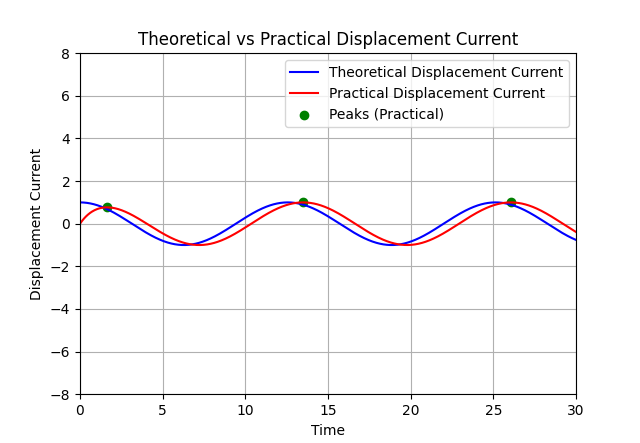
\includegraphics[width=\columnwidth]{2022/EC/24/figs/Figure_2.png}
    \caption{Thoritical vs Practical simulation}
    \label{fig:fig_gate_ec_2022_24_2}
\end{figure}

\begin{figure}[ht]
    \centering
    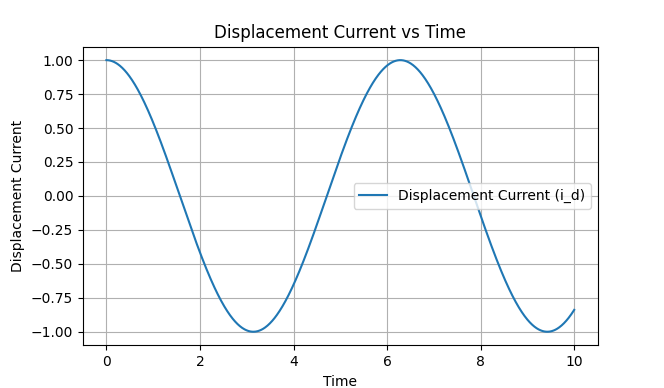
\includegraphics[width=\columnwidth]{2022/EC/24/figs/Figure_4.png}
    \caption{Displacement current}
    \label{fig:fig_gate_ec_2022_24_3}
\end{figure}



%\end{document}

\newpage

\item Given, $y=f\brak{x}$; $\frac{d^2y}{dx2}+4y=0; y\brak{0}=0; \frac{dy}{dx}\brak{0}=1$. The problem is a/an \\
\begin{enumerate}[label=(\alph*)]
    \item initial value problem having soluition $y=x$
    \item boundary value problem having soluition $y=x$
    \item initial value problem having soluition $y=\frac{1}{2}\sin 2x$
    \item boundary value problem having soluition {$y=\frac{1}{2}\sin 2x$}
\end{enumerate} \hfill(GATE 2022 ES)    \\
\solution
\iffalse
\let\negmedspace\undefined
\let\negthickspace\undefined
\documentclass[journal,12pt,twocolumn]{IEEEtran}
\usepackage{cite}
\usepackage{amsmath,amssymb,amsfonts,amsthm}
\usepackage{algorithmic}
\usepackage{graphicx}
\usepackage{textcomp}
\usepackage{xcolor}
\usepackage{txfonts}
\usepackage{listings}
\usepackage{enumitem}
\usepackage{mathtools}
\usepackage{gensymb}
\usepackage{comment}
\usepackage[breaklinks=true]{hyperref}
\usepackage{tkz-euclide} 
\usepackage{listings}
\usepackage{gvv}                                        
\def\inputGnumericTable{}                                 
\usepackage[latin1]{inputenc}                                
\usepackage{color}                                            
\usepackage{array}                                            
\usepackage{longtable}                                       
\usepackage{calc}                                             
\usepackage{multirow}                                         
\usepackage{hhline}                                           
\usepackage{ifthen}                                           
\usepackage{lscape}

\newtheorem{theorem}{Theorem}[section]
\newtheorem{problem}{Problem}
\newtheorem{proposition}{Proposition}[section]
\newtheorem{lemma}{Lemma}[section]
\newtheorem{corollary}[theorem]{Corollary}
\newtheorem{example}{Example}[section]
\newtheorem{definition}[problem]{Definition}
\newcommand{\BEQA}{\begin{eqnarray}}
\newcommand{\EEQA}{\end{eqnarray}}
\newcommand{\define}{\stackrel{\triangle}{=}}
\theoremstyle{remark}
\newtheorem{rem}{Remark}
\begin{document}
\parindent 0px
\bibliographystyle{IEEEtran}
\title{GATE: ES - 36.2022}
\author{EE22BTECH11219 - Rada Sai Sujan$^{}$% <-this % stops a space
}
\maketitle
\newpage
\bigskip
\section*{Question}
Given, $y=f\brak{x}$; $\frac{d^2y}{dx2}+4y=0; y\brak{0}=0; \frac{dy}{dx}\brak{0}=1$. The problem is a/an \\
\begin{enumerate}[label=(\alph*)]
    \item initial value problem having soluition $y=x$
    \item boundary value problem having soluition $y=x$
    \item initial value problem having soluition $y=\frac{1}{2}\sin 2x$
    \item boundary value problem having soluition {$y=\frac{1}{2}\sin 2x$}
\end{enumerate} \hfill(GATE 2022 ES)    \\
\solution
\fi

The above equation can be written as,
\begin{align}
    y^{\prime\prime}\brak{t}+4y\brak{t}=0
\end{align}
Using the Laplace transformation pairs,
\begin{align}
    y^{\prime\prime}\brak{t} &\overset{\mathcal{L}}{ \longleftrightarrow} s^2Y\brak{s}-sy\brak{0}-y^{\prime}\brak{0}    \\
    y\brak{t} &\overset{\mathcal{L}}{ \longleftrightarrow} Y\brak{s}    \\
    \sin at &\overset{\mathcal{L}}{ \longleftrightarrow} \frac{a}{a^2+s^2}  \label{equation:gate.es.2022.4}
\end{align}
Applying Laplace transform for the equation we get,
\begin{align}
    s^2Y\brak{s}-1+4Y\brak{s} &= 0  \\
    \implies Y\brak{s} &= \frac{1}{4+s^2}
\end{align}
Now, applying inverse laplace transform we get,
\begin{align}
    y\brak{t} &= \frac{1}{2}\sin 2t \quad \text{(from \eqref{equation:gate.es.2022.4})}
\end{align}
Since, the conditions at the same point\brak{0} are mentioned, it is an initial valued problem having solution $y=\frac{1}{2}\sin 2x$.
\begin{figure}[ht]
    \centering
    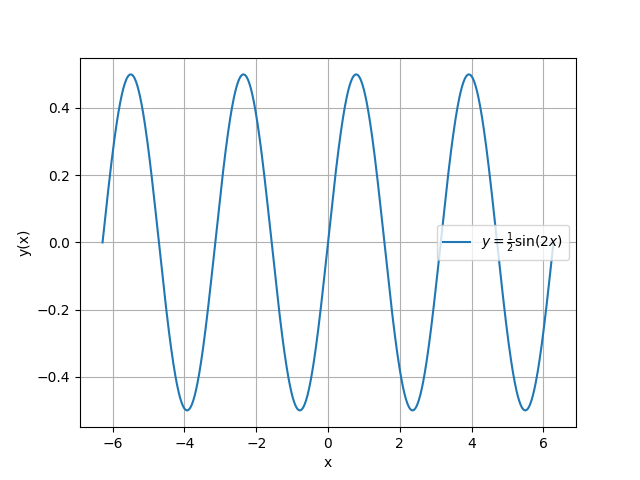
\includegraphics[width=\columnwidth]{2022/ES/36/figs/a.png}
    \caption{$y\brak{x}$ $vs$ $x$ graph}
    \label{figure:gate.2022.es.36Q.1}
\end{figure}

\newpage
\item Let a causal LTI system be governed by the following differential equation, 
\begin{align}
    y\brak{t} + \frac{1}{4}\frac{dy}{dt} = 2x\brak{t} \label{eq1}
\end{align}
where $x\brak{t}$ and $y\brak{t}$ are the input and output respectively. It's impulse response is 
\hfill (GATE EE-2022)\\
\solution
\iffalse
\let\negmedspace\undefined
\let\negthickspace\undefined
\documentclass[journal,12pt,twocolumn]{IEEEtran}
\usepackage{cite}
\usepackage{amsmath,amssymb,amsfonts,amsthm}
\usepackage{algorithmic}
\usepackage{graphicx}
\usepackage{textcomp}
\usepackage{xcolor}
\usepackage{txfonts}
\usepackage{listings}
\usepackage{enumitem}
\usepackage{mathtools}
\usepackage{gensymb}
\usepackage{comment}
\usepackage[breaklinks=true]{hyperref}
\usepackage{tkz-euclide} 
\usepackage{listings}
\usepackage{gvv}                                        
\def\inputGnumericTable{}                                 
\usepackage[latin1]{inputenc}                                
\usepackage{color}                                            
\newtheorem{theorem}{Theorem}[section]
\usepackage{array}                                            
\usepackage{longtable}                                       
\usepackage{calc}                                             
\usepackage{multirow}                                         
\usepackage{hhline}                                           
\usepackage{ifthen}                                           
\usepackage{lscape}
\newtheorem{problem}{Problem}
\newtheorem{proposition}{Proposition}[section]
\newtheorem{lemma}{Lemma}[section]
\newtheorem{corollary}[theorem]{Corollary}
\newtheorem{example}{Example}[section]
\newtheorem{definition}[problem]{Definition}
\newcommand{\BEQA}{\begin{eqnarray}}
\newcommand{\EEQA}{\end{eqnarray}}
\newcommand{\define}{\stackrel{\triangle}{=}}
\theoremstyle{remark}
\newtheorem{rem}{Remark}
\begin{document}
\bibliographystyle{IEEEtran}
\vspace{3cm}
\title{GATE 22 EE/46}
\author{EE23BTECH11040 - Manoj Kumar Ambatipudi$^{*}$% <-this % stops a space
}
\maketitle
\newpage
\bigskip
\renewcommand{\thefigure}{\theenumi}
\renewcommand{\thetable}{\theenumi}
\textbf{QUESTION:}
Let a causal LTI system be governed by the following differential equation, 
\begin{align}
    y\brak{t} + \frac{1}{4}\frac{dy}{dt} = 2x\brak{t} \label{eq1}
\end{align}
where $x\brak{t}$ and $y\brak{t}$ are the input and output respectively. It's impulse response is 
\hfill (GATE EE-2022)\\
\fi
\textbf{Solution:}

From \eqref{eq1}, corresponding Laplace transform, 
\begin{align}
    Y\brak{s} + \frac{1}{4}\brak{sY\brak{s} - y\brak{0}} = 2X\brak{s}
\end{align}
Since it is causal LTI system, 
\begin{align}
    y\brak{0} &= 0\\
	\implies Y\brak{s} + \frac{1}{4}sY\brak{s} &= 2X\brak{s}\\
    \implies Y\brak{s} &= X\brak{s}\frac{8}{4 + s}\\
    \implies H\brak{s} &= \frac{8}{4 + s}\quad ROC:Re\brak{s} > -4
\end{align}
Taking inverse laplace transform and applying causality conditions 
\begin{align}
    h\brak{t} = 8e^{-4t}u\brak{t}
\end{align}
\begin{figure}[h]
\renewcommand\thefigure{1}
    \centering
    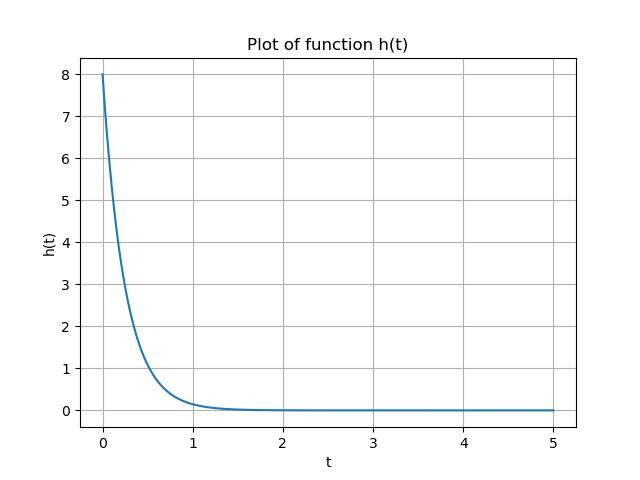
\includegraphics[width=1.0\columnwidth]{2022/EE/46/figs/fig_1.jpg}
    \caption{Plot of $h\brak{n}$, taken from python3}
    \label{fig:1}
\end{figure}


\item Assuming $s>0$; Laplace transform for $f\brak{x} = sin\brak{ax}$ is
\begin{enumerate}[label=(\Alph*)]
    \item $\frac{a}{s^2+a^2}$
    \item $\frac{s}{s^2+a^2}$
    \item $\frac{a}{s^2-a^2}$
    \item $\frac{s}{s^2-a^2}$
\end{enumerate} \hfill(GATE 2022 ES)\\
\solution
\iffalse
\let\negmedspace\undefined
\let\negthickspace\undefined
\documentclass[journal,12pt,twocolumn]{IEEEtran}
\usepackage{cite}
\usepackage{amsmath,amssymb,amsfonts,amsthm}
\usepackage{algorithmic}
\usepackage{graphicx}
\usepackage{textcomp}
\usepackage{xcolor}
\usepackage{txfonts}
\usepackage{listings}
\usepackage{enumitem}
\usepackage{mathtools}
\usepackage{gensymb}
\usepackage{comment}
\usepackage[breaklinks=true]{hyperref}
\usepackage{tkz-euclide} 
\usepackage{listings}
\usepackage{gvv}
\def\inputGnumericTable{}                                 
\usepackage[latin1]{inputenc}                                
\usepackage{color}                                            
\usepackage{array}                                            
\usepackage{longtable}                                       
\usepackage{calc}                                             
\usepackage{multirow}                                         
\usepackage{hhline}                                           
\usepackage{ifthen}                                           
\usepackage{lscape}

\newtheorem{theorem}{Theorem}[section]
\newtheorem{problem}{Problem}
\newtheorem{proposition}{Proposition}[section]
\newtheorem{lemma}{Lemma}[section]
\newtheorem{corollary}[theorem]{Corollary}
\newtheorem{example}{Example}[section]
\newtheorem{definition}[problem]{Definition}
\newcommand{\BEQA}{\begin{eqnarray}}
\newcommand{\EEQA}{\end{eqnarray}}
\newcommand{\define}{\stackrel{\triangle}{=}}
\theoremstyle{remark}
\newtheorem{rem}{Remark}

\begin{document}

\bibliographystyle{IEEEtran}
\vspace{3cm}

\title{GATE ES22 13}
\author{EE23BTECH11043 - BHUVANESH SUNIL NEHETE$^{*}$% <-this % stops a space
}
\maketitle
\newpage
\bigskip

\renewcommand{\thefigure}{\theenumi}
\renewcommand{\thetable}{\theenumi}

\bibliographystyle{IEEEtran}

\textbf{Question:}
Assuming $s>0$; Laplace transform for $f\brak{x} = sin\brak{ax}$ is
\begin{enumerate}[label=(\Alph*)]
    \item $\frac{a}{s^2+a^2}$
    \item $\frac{s}{s^2+a^2}$
    \item $\frac{a}{s^2-a^2}$
    \item $\frac{s}{s^2-a^2}$
\end{enumerate}

\solution
\fi
\begin{align}
\mathcal{L}\brak{f\brak{x}}=\int_{-\infty}^{\infty}e^{-sx}f\brak{x}dx\\
\text{We can write} \quad\sin\brak{ax}=\frac{e^{ax}-e^{-ax}}{2i}\label{13es22eq1}
\end{align}
From \eqref{13es22eq1}
\begin{align}
\mathcal{L}\brak{\sin\brak{ax}}&=\int_{0}^{\infty}e^{-sx}\brak{\frac{e^{iax}-e^{-iax}}{2i}}dx\\
&=\frac{1}{2i}\int_{0}^{\infty}e^{-x\brak{s-ia}}-e^{-x\brak{s+ia}}dx\\
&=\frac{1}{2i}\brak{\frac{e^{-x\brak{s-ia}}}{-\brak{s-ia}}+\frac{e^{-x\brak{s+ia}}}{-\brak{s+ia}}}_{0}^{\infty}\\
&=\frac{1}{2i}\brak{\frac{1}{s-ia}-\frac{1}{s+ia}}\\
&=\frac{a}{s^2+a^2}
\end{align}

So, option \brak{A} is correct.

\newpage

\end{enumerate}

 \section{2021}
 \begin{enumerate}[label=\thechapter.\arabic*,ref=\thechapter.\theenumi]
\item For the ordinary differential equation
\begin{align*}
\frac{d^3y}{dt^3} + 6\frac{d^2y}{dt^2} + 11\frac{dy}{dt} + 6y = 1,
\end{align*}
with initial conditions $y(0) = y'(0) = y''(0) = y'''(0) = 0$, the value of 
\begin{align*}
\lim_{{t \to \infty}} y(t) &= ?
\end{align*}
(round off to $3$ decimal places).
\hfill(GATE CH 2021)\\
\solution
\iffalse
\documentclass[journal,12pt,onecolumn]{IEEEtran}
\usepackage{cite}
\usepackage{amsmath,amssymb,amsfonts,amsthm}
\usepackage{algorithmic}
\usepackage{graphicx}
\usepackage{textcomp}
\usepackage{xcolor}
\usepackage{txfonts}
\usepackage{listings}
\usepackage{enumitem}
\usepackage{mathtools}
\usepackage{gensymb}
\usepackage{comment}
\usepackage[breaklinks=true]{hyperref}
\usepackage{tkz-euclide}
\usepackage{braket}
\def\inputGnumericTable{}
\usepackage[latin1]{inputenc}
\usepackage{color}
\usepackage{array}
\usepackage{longtable}
\usepackage{calc}
\usepackage{multirow}
\usepackage{hhline}
\usepackage{ifthen}
\usepackage{lscape}
\usepackage{gvv} 
\usepackage{circuitikz}

\newtheorem{theorem}{Theorem}[section]
\newtheorem{problem}{Problem}
\newtheorem{proposition}{Proposition}[section]
\newtheorem{lemma}{Lemma}[section]
\newtheorem{corollary}[theorem]{Corollary}
\newtheorem{example}{Example}[section]
\newtheorem{definition}[problem]{Definition}
\newcommand{\BEQA}{\begin{eqnarray}}
\newcommand{\EEQA}{\end{eqnarray}}
\newcommand{\define}{\stackrel{\triangle}{=}}
\theoremstyle{remark}
\newtheorem{rem}{Remark}
\renewcommand{\brak}[1]{\left(#1\right)}
\begin{document}

\bibliographystyle{IEEEtran}
\vspace{3cm}

\title{GATE 2021 CH-36}
\author{EE23BTECH11201 - Abburi Tanusha$^{*}$% <-this % stops a space
}
\maketitle

\renewcommand{\thefigure}{\theenumi}
\renewcommand{\thetable}{\theenumi}

\vspace{3cm}

\maketitle
\textbf{Question:} 
For the ordinary differential equation
\begin{align*}
\frac{d^3y}{dt^3} + 6\frac{d^2y}{dt^2} + 11\frac{dy}{dt} + 6y = 1,
\end{align*}
with initial conditions $y(0) = y'(0) = y''(0) = y'''(0) = 0$, the value of 
\begin{align*}
\lim_{{t \to \infty}} y(t) &= ?
\end{align*}
(round off to $3$ decimal places).
\hfill(GATE CH 2021)\\
\textbf{Solution:} 
\fi
\begin{table}[h]
 	\centering
 	\resizebox{6 cm}{!}{
 		
\begin{tabular}{|c|c|l|}
\hline
Parameter  & Value & Description   \\             
\hline
$y(0)$     & $0$   & Initial displacement  \\     
 \hline
$y'(0)$    & $0$   & First derivative at $t=0$  \\
 \hline
$y''(0)$   & $0$   & Second derivative at $t=0$ \\
 \hline
$y'''(0)$  & $0$   & Third derivative at $t=0$  \\
 \hline
\end{tabular}


 	}
 	\vspace{6 pt}
 	\caption{Parameters}
 \end{table}
\begin{align}
\frac{d^3y}{dt^3} + 6\frac{d^2y}{dt^2} + 11\frac{dy}{dt} + 6y &= 1
\end{align}
Applying the Laplace transform to both sides:
\begin{align}
s^3Y(s) + 6s^2Y(s) + 11sY(s) + 6Y(s) &= \frac{1}{s} \\
Y(s)\brak{s^3 + 6s^2 + 11s + 6} &= \frac{1}{s} \\
\implies Y(s) &= \frac{1}{s\brak{s+1}\brak{s+2}\brak{s+3}} ; \quad Re(s) > 0
\end{align}
\begin{align}
Y(s) &= \frac{A}{s} + \frac{B}{s+1} + \frac{C}{s+2} + \frac{D}{s+3} \\
1 &= A\brak{s+1}\brak{s+2}\brak{s+3} + Bs\brak{s+2}\brak{s+3} + Cs\brak{s+1}\brak{s+3} + Ds\brak{s+1}\brak{s+2}  \\
1 &= A\brak{s^3 + 6s^2 + 11s + 6} + Bs\brak{s^2 + 5s + 6}  + Cs\brak{s^2 + 4s + 3} + Ds\brak{s^2 + 3s + 2} \\
\end{align}
Comparing the coefficients on both sides \\
\begin{align}
A + B + C + D = 0 \\
6A + 5B + 4C + 3D = 0 \\
11A + 6B + 3C + 2D = 0 \\
6A = 1 \\
A=1/6 ,B = -11/26 , C= 5/26 , D= 5/78 
\end{align}
Substitute these values 
\begin{align}
Y(s) = \frac{6}{s} - \frac{11}{26\brak{s+1}} + \frac{5}{26\brak{s+2}} + \frac{5}{78\brak{s+3}}
\end{align}
Apply Inverse Laplace Transform 
\begin{align}
y(t) &= 6\mathcal{L}^{-1}\brak{\frac{1}{s}} - 11\mathcal{L}^{-1}\brak{\frac{1}{26\brak{s+1}}} + 5\mathcal{L}^{-1}\brak{\frac{1}{26\brak{s+2}}} + 5\mathcal{L}^{-1}\brak{\frac{1}{78\brak{s+3}}} \\
y(t) &= 6 - \frac{11}{26}e^{-t} + \frac{5}{26}e^{-2t} +\frac{5}{78}e^{-3t}
\end{align}
Consider
\begin{align}
\lim_{t \to \infty} y(t) &= \lim_{t \to \infty} \brak{6 - \frac{11}{26}e^{-t} + \frac{5}{26}e^{-2t} +\frac{5}{78}e^{-3t}} \\
&= 6
\end{align}\
Verifying using Final Value Theorem :\\
\begin{align}
 \lim_{t \to \infty} y(t)   &= \lim_{s \to 0} sY(s)  \\
\lim_{s \to 0} sY(s) &= \lim_{s \to 0} s \brak{ \frac{6}{s} - \frac{11}{26\brak{s+1}} + \frac{5}{26\brak{s+2}} + \frac{5}{78\brak{s+3}}} \\
&= \lim_{s \to 0} \brak{ 6 - \frac{11s}{26\brak{s+1}} + \frac{5s}{26\brak{s+2}} + \frac{5s}{78\brak{s+3}}} \\
&= 6
\end{align}

\begin{figure}[h!]
\centering
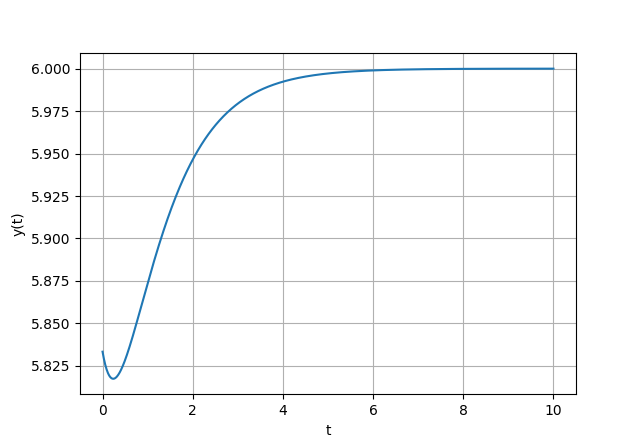
\includegraphics[width=\columnwidth]{2021/CH/36/figs/plot.png}
\caption{Plot $y(t)$ vs $t$ }
\end{figure}
%\end{document}

\pagebreak
\item \textbf{Question:}
Consider the differential equation \\$\frac{d^2y}{dx^2}+8\frac{dy}{dx}+16y=0$ and the boundary conditions $y(0)=1$ and $\frac{dy}{dx}(0)=0$. The solution to equation is:\\
\hfill{(GATE.AE-1.2021)}\\
\solution
 \iffalse
\let\negmedspace\undefined
\let\negthickspace\undefined
\documentclass[journal,12pt,twocolumn]{IEEEtran}
\usepackage{xparse}
\usepackage{cite}
\usepackage{amsmath,amssymb,amsfonts,amsthm}
\usepackage{algorithmic}
\usepackage{graphicx}
\usepackage{textcomp}
\usepackage{xcolor}
\usepackage{txfonts}
\usepackage{listings}
\usepackage{enumitem}
\usepackage{mathtools}
\usepackage{gensymb}
\usepackage{comment}
\usepackage[breaklinks=true]{hyperref}
\usepackage{tkz-euclide}
\usepackage{listings}
\usepackage{gvv}
\def\inputGnumericTable{}
\usepackage[latin1]{inputenc}
\usepackage{color}
\usepackage{array}
\usepackage{longtable}
\usepackage{calc}
\usepackage{multirow}
\usepackage{hhline}
\usepackage{ifthen}
\usepackage{lscape}
\begin{enumerate}[label=\thechapter.\arabic*,ref=\thechapter.\theenumi]
\numberwithin{equation}{enumi}
\numberwithin{figure}{enumi}
\numberwithin{table}{enumi}
\item Laplace Transform of Partial Differentials\\
Let a function $y\brak{x,t}$ be defined for all $t>0$ and assumed to be bounded. Appling Laplace transform in t considering x as a parameter,
\begin{align}
 \mathcal{L}\brak{y\brak{x,t}} &= \int_{0}^{\infty}e^{-st}y\brak{x,t}dt\\
 &= Y\brak{x,s}
\end{align}
Let $\dfrac{\partial y\brak{x,t}}{\partial t}$ be $y_t\brak{x,t}$ and $\dfrac{\partial y\brak{x,t}}{\partial x}$ be $y_x\brak{x,t}$, then
\begin{align}
 \mathcal{L}\brak{y_t\brak{x,t}} &= \int_{0}^{\infty}e^{-st}y_t\brak{x,t}dt\\
 &= \left. e^{-st}y\brak{x,t}\right|_{0}^{\infty} + s\int_{0}^{\infty}e^{-st} y\brak{x,t} dt\\
 &= sY\brak{x,s} - y\brak{x,0} \label{L(y_t(x,t))}\\
 \mathcal{L}\brak{y_x\brak{x,t}} &= \int_{0}^{\infty}e^{-st}y_x\brak{x,t}dt\\
 &= \dfrac{d}{dx}\int_{0}^{\infty}e^{-st}y\brak{x,t}dt \label{L(y_x(x,t))}\\
 &= \dfrac{dY\brak{x,s}}{dx}
\end{align}
\item Laplace transform of f(t):
\begin{align}
        f(t)u(t)\system{L}&\int_{0}^{\infty}f(t)e^{-st}\; dt\\
        &=F(s)\label{lap transform}
\end{align}
\item Laplace transform of powers of $t$\\
        Let $f(t)=t^nu(t)$\\
From \eqref{lap transform},and considering $h=st$
\begin{align}
        F(s)&=\frac{1}{s^{n+1}}\int_{0}^{\infty}h^ne^{-h}\;dh\label{lap 1}\\
        (n-1)!&=\int_0^\infty e^{-t}t^{n-1}\;dt\text{ (Gamma function)}\label{gamma}
\end{align}
From \eqref{lap 1},\eqref{gamma}
\begin{align}
        F(s)&=\frac{n!}{s^{n+1}}\\
         t^nu(t)&\system{L}\frac{n!}{s^{n+1}}\label{lap exp}
\end{align}
\item Frequency shift property:\\
        Let $f(t)=y(t)e^{-at}u(t)$\\
From\eqref{lap transform},
\begin{align}
        F(s)&=\int_0^{\infty}y(t)e^{-(s+a)t}\;dt\\
         y(t)e^{-at}u(t)&\system{L}Y(s+a)\label{lap freq shift}
\end{align}
\item Inverse Laplace for partial fractions\\
From \eqref{lap exp},\eqref{lap freq shift} we get
\begin{align}
    &\frac{b}{(s+a)^n}\xleftrightarrow{\mathcal{L}^{-1}}\frac{b}{(n-1)!}\cdot t^{n-1} e^{-at}\cdot u(t)\label{inv lap (partial fractions)}
\end{align}
\item Laplace transform of derivatives:\\
        Let $f(t)=y'(t)u(t)$\\
From \eqref{lap transform}, integration by parts,recursion
\begin{align}
        F(s)&=\int_{0}^\infty e^{-st}\; dy\\
        &=[y(t)e^{-st}]_0^\infty+s\int_0^\infty y(t)e^{-st}dt\\
        &=-y(0)+sY(s)\label{lap 2}
\end{align}
From\eqref{lap 2},recursion
\begin{align}
        y'(t)u(t)&\system{L}sY(s)-\int y'(t)\;dt\vert_{t=0}\\
        y^{(n)}(t)u(t)&\system{L}s^nY(s)-\sum\limits_{k=0}^{n-1}s^{(n-1-k)}y^{(k)}(0)\label{lap (derivatives)}
\end{align}

\item Laplace transform of integrals:\\
Let the function defined as $y(t) = \int_0^t f(u) du$ for all $t > 0$\\
Laplace transform of y(t) in t 
\begin{align}
    \mathcal{L} \brak{y(t)} &= \int_0^{\infty} e^{-st} y(t) dt\\
    &= \int_0^{\infty} e^{-st} \int_0^t f(u) du dt\\
    &= \int_0^t f(u) du \sbrak{- \frac{e^{-st}}{s}}_0^{\infty} + \int_0^{\infty} \frac{e^{-st}}{s} f(t) dt\\
    &= \frac{F(s)}{s}
\end{align}


\end{enumerate}

\newtheorem{theorem}{Theorem}[section]
\newtheorem{problem}{Problem}
\newtheorem{proposition}{Proposition}[section]
\newtheorem{lemma}{Lemma}[section]
\newtheorem{corollary}[theorem]{Corollary}
\newtheorem{example}{Example}[section]
\newtheorem{definition}[problem]{Definition}
\newcommand{\BEQA}{\begin{eqnarray}}
\newcommand{\EEQA}{\end{eqnarray}}
\newcommand{\define}{\stackrel{\triangle}{=}}
\theoremstyle{remark}
\newtheorem{rem}{Remark}
\begin{document}

\bibliographystyle{IEEEtran}
\vspace{3cm}

\title{GATE-AE.1}
\author{EE23BTECH11046 - Poluri Hemanth$^{*}$}
\maketitle
\textbf{Question:}
Consider the differential equation \\$\frac{d^2y}{dx^2}+8\frac{dy}{dx}+16y=0$ and the boundary conditions $y(0)=1$ and $\frac{dy}{dx}(0)=0$. The solution to equation is:\\
\hfill{(GATE.AE-1.2021)}\\
\textbf{Solution:}\\
\fi
\begin{table}[h!]
    % Change address in github
        %%%%%%%%%%%%%%%%%%%%%%%%%%%%%%%%%%%%%%%%%%%%%%%%%%%%%%%%%%%%%%%%%%%%%%
%%                                                                  %%
%%  This is the header of a LaTeX2e file exported from Gnumeric.    %%
%%                                                                  %%
%%  This file can be compiled as it stands or included in another   %%
%%  LaTeX document. The table is based on the longtable package so  %%
%%  the longtable options (headers, footers...) can be set in the   %%
%%  preamble section below (see PRAMBLE).                           %%
%%                                                                  %%
%%  To include the file in another, the following two lines must be %%
%%  in the including file:                                          %%
%%        \def\inputGnumericTable{}                                 %%
%%  at the beginning of the file and:                               %%
%%        \input{name-of-this-file.tex}                             %%
%%  where the table is to be placed. Note also that the including   %%
%%  file must use the following packages for the table to be        %%
%%  rendered correctly:                                             %%
%%    \usepackage[latin1]{inputenc}                                 %%
%%    \usepackage{color}                                            %%
%%    \usepackage{array}                                            %%
%%    \usepackage{longtable}                                        %%
%%    \usepackage{calc}                                             %%
%%    \usepackage{multirow}                                         %%
%%    \usepackage{hhline}                                           %%
%%    \usepackage{ifthen}                                           %%
%%  optionally (for landscape tables embedded in another document): %%
%%    \usepackage{lscape}                                           %%
%%                                                                  %%
%%%%%%%%%%%%%%%%%%%%%%%%%%%%%%%%%%%%%%%%%%%%%%%%%%%%%%%%%%%%%%%%%%%%%%



%%  This section checks if we are begin input into another file or  %%
%%  the file will be compiled alone. First use a macro taken from   %%
%%  the TeXbook ex 7.7 (suggestion of Han-Wen Nienhuys).            %%
\def\ifundefined#1{\expandafter\ifx\csname#1\endcsname\relax}


%%  Check for the \def token for inputed files. If it is not        %%
%%  defined, the file will be processed as a standalone and the     %%
%%  preamble will be used.                                          %%
\ifundefined{inputGnumericTable}

%%  We must be able to close or not the document at the end.        %%
	\def\gnumericTableEnd{\end{document}}


%%%%%%%%%%%%%%%%%%%%%%%%%%%%%%%%%%%%%%%%%%%%%%%%%%%%%%%%%%%%%%%%%%%%%%
%%                                                                  %%
%%  This is the PREAMBLE. Change these values to get the right      %%
%%  paper size and other niceties.                                  %%
%%                                                                  %%
%%%%%%%%%%%%%%%%%%%%%%%%%%%%%%%%%%%%%%%%%%%%%%%%%%%%%%%%%%%%%%%%%%%%%%

	\documentclass[12pt%
			  %,landscape%
                    ]{report}
       \usepackage[latin1]{inputenc}
       \usepackage{fullpage}
       \usepackage{color}
       \usepackage{array}
       \usepackage{longtable}
       \usepackage{calc}
       \usepackage{multirow}
       \usepackage{hhline}
       \usepackage{ifthen}

	\begin{document}


%%  End of the preamble for the standalone. The next section is for %%
%%  documents which are included into other LaTeX2e files.          %%
\else

%%  We are not a stand alone document. For a regular table, we will %%
%%  have no preamble and only define the closing to mean nothing.   %%
    \def\gnumericTableEnd{}

%%  If we want landscape mode in an embedded document, comment out  %%
%%  the line above and uncomment the two below. The table will      %%
%%  begin on a new page and run in landscape mode.                  %%
%       \def\gnumericTableEnd{\end{landscape}}
%       \begin{landscape}


%%  End f the else clause for this file being \input.              %%
\fi

%%%%%%%%%%%%%%%%%%%%%%%%%%%%%%%%%%%%%%%%%%%%%%%%%%%%%%%%%%%%%%%%%%%%%%
%%                                                                  %%
%%  The rest is the gnumeric table, except for the closing          %%
%%  statement. Changes below will alter the table's appearance.     %%
%%                                                                  %%
%%%%%%%%%%%%%%%%%%%%%%%%%%%%%%%%%%%%%%%%%%%%%%%%%%%%%%%%%%%%%%%%%%%%%%

\providecommand{\gnumericmathit}[1]{#1} 
%%  Uncomment the next line if you would like your numbers to be in %%
%%  italics if they are italizised in the gnumeric table.           %%
%\renewcommand{\gnumericmathit}[1]{\mathit{#1}}
\providecommand{\gnumericPB}[1]%
{\let\gnumericTemp=\\#1\let\\=\gnumericTemp\hspace{0pt}}
 \ifundefined{gnumericTableWidthDefined}
        \newlength{\gnumericTableWidth}
        \newlength{\gnumericTableWidthComplete}
        \newlength{\gnumericMultiRowLength}
        \global\def\gnumericTableWidthDefined{}
 \fi
%% The following setting protects this code from babel shorthands.  %%
 \ifthenelse{\isundefined{\languageshorthands}}{}{\languageshorthands{english}}
%%  The default table format retains the relative column widths of  %%
%%  gnumeric. They can easily be changed to c, r or l. In that case %%
%%  you may want to comment out the next line and uncomment the one %%
%%  thereafter                                                      %%
\providecommand\gnumbox{\makebox[0pt]}
%%\providecommand\gnumbox[1][]{\makebox}

%% to adjust positions in multirow situations                       %%
\setlength{\bigstrutjot}{\jot}
\setlength{\extrarowheight}{\doublerulesep}

%%  The \setlongtables command keeps column widths the same across  %%
%%  pages. Simply comment out next line for varying column widths.  %%
\setlongtables

\setlength\gnumericTableWidth{%
	20pt+%
	40pt+%
	50pt+%	
0pt}
\def\gumericNumCols{3}
\setlength\gnumericTableWidthComplete{\gnumericTableWidth+%
         \tabcolsep*\gumericNumCols*2+\arrayrulewidth*\gumericNumCols}
\ifthenelse{\lengthtest{\gnumericTableWidthComplete > \linewidth}}%
         {\def\gnumericScale{1*\ratio{\linewidth-%
                        \tabcolsep*\gumericNumCols*2-%
                        \arrayrulewidth*\gumericNumCols}%
{\gnumericTableWidth}}}%
{\def\gnumericScale{2}}

%%%%%%%%%%%%%%%%%%%%%%%%%%%%%%%%%%%%%%%%%%%%%%%%%%%%%%%%%%%%%%%%%%%%%%
%%                                                                  %%
%% The following are the widths of the various columns. We are      %%
%% defining them here because then they are easier to change.       %%
%% Depending on the cell formats we may use them more than once.    %%
%%                                                                  %%
%%%%%%%%%%%%%%%%%%%%%%%%%%%%%%%%%%%%%%%%%%%%%%%%%%%%%%%%%%%%%%%%%%%%%%

\ifthenelse{\isundefined{\gnumericColA}}{\newlength{\gnumericColA}}{}\settowidth{\gnumericColA}{\begin{tabular}{@{}p{20pt*\gnumericScale}@{}}x\end{tabular}}
\ifthenelse{\isundefined{\gnumericColB}}{\newlength{\gnumericColB}}{}\settowidth{\gnumericColB}{\begin{tabular}{@{}p{40pt*\gnumericScale}@{}}x\end{tabular}}
\ifthenelse{\isundefined{\gnumericColC}}{\newlength{\gnumericColC}}{}\settowidth{\gnumericColC}{\begin{tabular}{@{}p{50pt*\gnumericScale}@{}}x\end{tabular}}

\begin{tabular}[c]{%
	b{\gnumericColA}%
	b{\gnumericColB}%
	b{\gnumericColC}%
	}

%%%%%%%%%%%%%%%%%%%%%%%%%%%%%%%%%%%%%%%%%%%%%%%%%%%%%%%%%%%%%%%%%%%%%%
%%  The longtable options. (Caption, headers... see Goosens, p.124) %%
%	\caption{The Table Caption.}             \\	%
% \hline	% Across the top of the table.
%%  The rest of these options are table rows which are placed on    %%
%%  the first, last or every page. Use \multicolumn if you want.    %%

%%  Header for the first page.                                      %%
%	\multicolumn{3}{c}{The First Header} \\ \hline 
%	\multicolumn{1}{c}{colTag}	%Column 1
%	&\multicolumn{1}{c}{colTag}	%Column 2
%	&\multicolumn{1}{c}{colTag}	\\ \hline %Last column
%	\endfirsthead

%%  The running header definition.                                  %%
%	\hline
%	\multicolumn{3}{l}{\ldots\small\slshape continued} \\ \hline
%	\multicolumn{1}{c}{colTag}	%Column 1
%	&\multicolumn{1}{c}{colTag}	%Column 2
%	&\multicolumn{1}{c}{colTag}	\\ \hline %Last column
%	\endhead

%%  The running footer definition.                                  %%
%	\hline
%	\multicolumn{3}{r}{\small\slshape continued\ldots} \\
%	\endfoot

%%  The ending footer definition.                                   %%
%	\multicolumn{3}{c}{That's all folks} \\ \hline 
%	\endlastfoot
%%%%%%%%%%%%%%%%%%%%%%%%%%%%%%%%%%%%%%%%%%%%%%%%%%%%%%%%%%%%%%%%%%%%%%
\hhline{|-|-|-}
	\multicolumn{1}{|p{\gnumericColA}|}%
	{\gnumericPB{\centering}\gnumbox{\textbf{Symbol}}}
	&\multicolumn{1}{p{\gnumericColB}|}%
	{\gnumericPB{\centering}\gnumbox{\textbf{Values}}}
	&\multicolumn{1}{p{\gnumericColC}|}%
	{\gnumericPB{\centering}\gnumbox{\textbf{Description}}}

\\
\hhline{|---|}
	\multicolumn{1}{|p{\gnumericColA}|}%
	{\gnumericPB{\centering}\gnumbox{$Y(s)$}}
	&\multicolumn{1}{p{\gnumericColB}|}%
	{\gnumericPB{\centering}\gnumbox{-}}
	&\multicolumn{1}{p{\gnumericColC}|}%
	{\gnumericPB{\centering}\gnumbox{$y$ in s domain}}

\\
\hhline{|---|}
        \multicolumn{1}{|p{\gnumericColA}|}%
	{\gnumericPB{\centering}\gnumbox{$y(x)$}}             
        &\multicolumn{1}{p{\gnumericColB}|}%
	{\gnumericPB{\centering}\gnumbox{-}}  
        &\multicolumn{1}{p{\gnumericColC}|}%
	{\gnumericPB{\centering}\gnumbox{$y$ in x domain}}

\\
\hhline{|---|}
        \multicolumn{1}{|p{\gnumericColA}|}%
        {\gnumericPB{\centering}\gnumbox{$y(0)$}}             
        &\multicolumn{1}{p{\gnumericColB}|}%
        {\gnumericPB{\centering}\gnumbox{1}}  
        &\multicolumn{1}{p{\gnumericColC}|}%
        {\gnumericPB{\centering}\gnumbox{$y$ at $x=0$}}
\\
\hhline{|---|}
        \multicolumn{1}{|p{\gnumericColA}|}%
        {\gnumericPB{\centering}\gnumbox{$y'(0)$}}             
        &\multicolumn{1}{p{\gnumericColB}|}%
        {\gnumericPB{\centering}\gnumbox{0}}  
        &\multicolumn{1}{p{\gnumericColC}|}%
	{\gnumericPB{\centering}\gnumbox{$y'(x)$ at $x=0$}}

\\
\hhline{|---|}
        \multicolumn{1}{|p{\gnumericColA}|}%
	{\gnumericPB{\centering}\gnumbox{$u(x)$}}             
        &\multicolumn{1}{p{\gnumericColB}|}%
	{\gnumericPB{\centering}\gnumbox{$=\begin{cases}
        1 & \text{if } x > 0\\
        0 &  o.w
    \end{cases}$}}  
        &\multicolumn{1}{p{\gnumericColC}|}%
        {\gnumericPB{\centering}\gnumbox{unit step function}}
\\
\hhline{|-|-|-|}
\end{tabular}

\ifthenelse{\isundefined{\languageshorthands}}{}{\languageshorthands{\languagename}}
\gnumericTableEnd

        \caption{Parameters}
        \label{tab:AE.1.2021}
\end{table}\\
From \ref{lap (derivatives)}
\begin{align}
	\frac{d^2y}{dx^2}+8\frac{dy}{dx}+16y&\Large\xleftrightarrow{\mathcal{L}}s^2Y(s)-sy(0)-y'(0)+8sY(s)-8y(0)+16Y(s)
\end{align}
\begin{align}
	Y(s)(s^2+8s+16)&=s+8
\end{align}
\begin{align}
	\Rightarrow Y(s)&=\frac{s+8}{s^2+8s+16}\\
	&=\frac{1}{s+4}+\frac{4}{(s+4)^2}\label{1ae.1}
\end{align}
For inversion of $Y(s)$ in partial fractions-
\\ From \ref{inv lap (partial fractions)}
\begin{align}
	&\frac{b}{(s+a)^n}\Large\xleftrightarrow{\mathcal{L}^{-1}}\frac{b}{(n-1)!}\cdot x^{n-1} e^{-ax}\cdot u(x)\label{invae.1}
\end{align}
\\
Applying Laplace inverse-\\
\\From \eqref{1ae.1},\eqref{invae.1}
\begin{align}
	y(x)&=\frac{1}{0!} e^{-4x}\cdot u(x)+\frac{4}{1!}x\cdot e^{-4x}\cdot u(x)\\
	&=(1+4x)e^{-4x}u(x)
\end{align}
\newpage
\begin{figure}[h!]
    \centering
    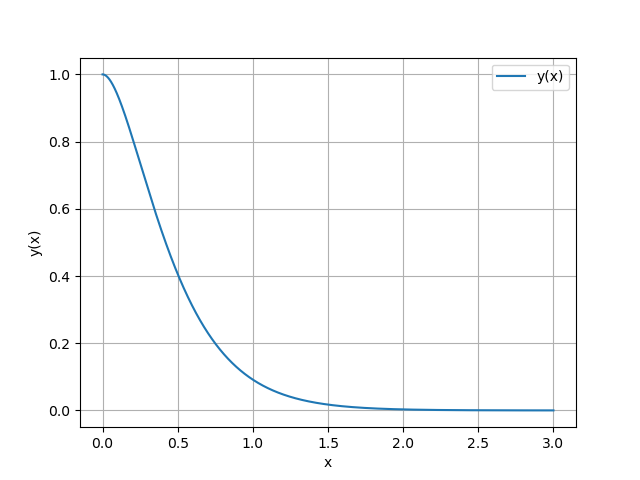
\includegraphics[width=1\linewidth]{2021/AE/1/figures/figure.png}
        \caption{Plot of y(x)}
    \label{fig:enter-label}
\end{figure}


%\end{document}






\pagebreak
\item\textbf{Question:}
The solution of second-order differential equation \\ $\frac{d^2y}{dx^2}+2\frac{dy}{dx}+y=0$ with boundary conditions $y(0)=1$ and $y(1)=3$.\\
\hfill{(GATE  2021 CE.26)}\\
\solution
\iffalse
\let\negmedspace\undefined
\let\negthickspace\undefined
\documentclass[journal,12pt,twocolumn]{IEEEtran}
\usepackage{xparse}
\usepackage{cite}
\usepackage{amsmath,amssymb,amsfonts,amsthm}
\usepackage{algorithmic}
\usepackage{graphicx}
\usepackage{textcomp}
\usepackage{xcolor}
\usepackage{txfonts}
\usepackage{listings}
\usepackage{enumitem}
\usepackage{mathtools}
\usepackage{gensymb}
\usepackage{comment}
\usepackage[breaklinks=true]{hyperref}
\usepackage{tkz-euclide}
\usepackage{listings}
\usepackage{gvv}
\def\inputGnumericTable{}
\usepackage[latin1]{inputenc}
\usepackage{color}
\usepackage{array}
\usepackage{longtable}
\usepackage{calc}
\usepackage{multirow}
\usepackage{hhline}
\usepackage{ifthen}
\usepackage{lscape}
\begin{enumerate}[label=\thechapter.\arabic*,ref=\thechapter.\theenumi]
\numberwithin{equation}{enumi}
\numberwithin{figure}{enumi}
\numberwithin{table}{enumi}
\item Laplace Transform of Partial Differentials\\
Let a function $y\brak{x,t}$ be defined for all $t>0$ and assumed to be bounded. Appling Laplace transform in t considering x as a parameter,
\begin{align}
 \mathcal{L}\brak{y\brak{x,t}} &= \int_{0}^{\infty}e^{-st}y\brak{x,t}dt\\
 &= Y\brak{x,s}
\end{align}
Let $\dfrac{\partial y\brak{x,t}}{\partial t}$ be $y_t\brak{x,t}$ and $\dfrac{\partial y\brak{x,t}}{\partial x}$ be $y_x\brak{x,t}$, then
\begin{align}
 \mathcal{L}\brak{y_t\brak{x,t}} &= \int_{0}^{\infty}e^{-st}y_t\brak{x,t}dt\\
 &= \left. e^{-st}y\brak{x,t}\right|_{0}^{\infty} + s\int_{0}^{\infty}e^{-st} y\brak{x,t} dt\\
 &= sY\brak{x,s} - y\brak{x,0} \label{L(y_t(x,t))}\\
 \mathcal{L}\brak{y_x\brak{x,t}} &= \int_{0}^{\infty}e^{-st}y_x\brak{x,t}dt\\
 &= \dfrac{d}{dx}\int_{0}^{\infty}e^{-st}y\brak{x,t}dt \label{L(y_x(x,t))}\\
 &= \dfrac{dY\brak{x,s}}{dx}
\end{align}
\item Laplace transform of f(t):
\begin{align}
        f(t)u(t)\system{L}&\int_{0}^{\infty}f(t)e^{-st}\; dt\\
        &=F(s)\label{lap transform}
\end{align}
\item Laplace transform of powers of $t$\\
        Let $f(t)=t^nu(t)$\\
From \eqref{lap transform},and considering $h=st$
\begin{align}
        F(s)&=\frac{1}{s^{n+1}}\int_{0}^{\infty}h^ne^{-h}\;dh\label{lap 1}\\
        (n-1)!&=\int_0^\infty e^{-t}t^{n-1}\;dt\text{ (Gamma function)}\label{gamma}
\end{align}
From \eqref{lap 1},\eqref{gamma}
\begin{align}
        F(s)&=\frac{n!}{s^{n+1}}\\
         t^nu(t)&\system{L}\frac{n!}{s^{n+1}}\label{lap exp}
\end{align}
\item Frequency shift property:\\
        Let $f(t)=y(t)e^{-at}u(t)$\\
From\eqref{lap transform},
\begin{align}
        F(s)&=\int_0^{\infty}y(t)e^{-(s+a)t}\;dt\\
         y(t)e^{-at}u(t)&\system{L}Y(s+a)\label{lap freq shift}
\end{align}
\item Inverse Laplace for partial fractions\\
From \eqref{lap exp},\eqref{lap freq shift} we get
\begin{align}
    &\frac{b}{(s+a)^n}\xleftrightarrow{\mathcal{L}^{-1}}\frac{b}{(n-1)!}\cdot t^{n-1} e^{-at}\cdot u(t)\label{inv lap (partial fractions)}
\end{align}
\item Laplace transform of derivatives:\\
        Let $f(t)=y'(t)u(t)$\\
From \eqref{lap transform}, integration by parts,recursion
\begin{align}
        F(s)&=\int_{0}^\infty e^{-st}\; dy\\
        &=[y(t)e^{-st}]_0^\infty+s\int_0^\infty y(t)e^{-st}dt\\
        &=-y(0)+sY(s)\label{lap 2}
\end{align}
From\eqref{lap 2},recursion
\begin{align}
        y'(t)u(t)&\system{L}sY(s)-\int y'(t)\;dt\vert_{t=0}\\
        y^{(n)}(t)u(t)&\system{L}s^nY(s)-\sum\limits_{k=0}^{n-1}s^{(n-1-k)}y^{(k)}(0)\label{lap (derivatives)}
\end{align}

\item Laplace transform of integrals:\\
Let the function defined as $y(t) = \int_0^t f(u) du$ for all $t > 0$\\
Laplace transform of y(t) in t 
\begin{align}
    \mathcal{L} \brak{y(t)} &= \int_0^{\infty} e^{-st} y(t) dt\\
    &= \int_0^{\infty} e^{-st} \int_0^t f(u) du dt\\
    &= \int_0^t f(u) du \sbrak{- \frac{e^{-st}}{s}}_0^{\infty} + \int_0^{\infty} \frac{e^{-st}}{s} f(t) dt\\
    &= \frac{F(s)}{s}
\end{align}


\end{enumerate}

\newtheorem{theorem}{Theorem}[section]
\newtheorem{problem}{Problem}
\newtheorem{proposition}{Proposition}[section]
\newtheorem{lemma}{Lemma}[section]
\newtheorem{corollary}[theorem]{Corollary}
\newtheorem{example}{Example}[section]
\newtheorem{definition}[problem]{Definition}
\newcommand{\BEQA}{\begin{eqnarray}}
\newcommand{\EEQA}{\end{eqnarray}}
\newcommand{\define}{\stackrel{\triangle}{=}}
\theoremstyle{remark}
\newtheorem{rem}{Remark}
\begin{document}

\bibliographystyle{IEEEtran}
\vspace{3cm}

\title{GATE-CE.26}
\author{EE23BTECH11046 - Poluri Hemanth$^{*}$}
\maketitle
\textbf{Question:}
The solution of second-order differential equation \\ $\frac{d^2y}{dx^2}+2\frac{dy}{dx}+y=0$ with boundary conditions $y(0)=1$ and $y(1)=3$.\\
\hfill{(GATE  2021 CE.26)}\\
\textbf{Solution:}
\fi
\begin{table}[h!]
    % Change address in github
        %%%%%%%%%%%%%%%%%%%%%%%%%%%%%%%%%%%%%%%%%%%%%%%%%%%%%%%%%%%%%%%%%%%%%%
%%                                                                  %%
%%  This is the header of a LaTeX2e file exported from Gnumeric.    %%
%%                                                                  %%
%%  This file can be compiled as it stands or included in another   %%
%%  LaTeX document. The table is based on the longtable package so  %%
%%  the longtable options (headers, footers...) can be set in the   %%
%%  preamble section below (see PRAMBLE).                           %%
%%                                                                  %%
%%  To include the file in another, the following two lines must be %%
%%  in the including file:                                          %%
%%        \def\inputGnumericTable{}                                 %%
%%  at the beginning of the file and:                               %%
%%        \input{name-of-this-file.tex}                             %%
%%  where the table is to be placed. Note also that the including   %%
%%  file must use the following packages for the table to be        %%
%%  rendered correctly:                                             %%
%%    \usepackage[latin1]{inputenc}                                 %%
%%    \usepackage{color}                                            %%
%%    \usepackage{array}                                            %%
%%    \usepackage{longtable}                                        %%
%%    \usepackage{calc}                                             %%
%%    \usepackage{multirow}                                         %%
%%    \usepackage{hhline}                                           %%
%%    \usepackage{ifthen}                                           %%
%%  optionally (for landscape tables embedded in another document): %%
%%    \usepackage{lscape}                                           %%
%%                                                                  %%
%%%%%%%%%%%%%%%%%%%%%%%%%%%%%%%%%%%%%%%%%%%%%%%%%%%%%%%%%%%%%%%%%%%%%%



%%  This section checks if we are begin input into another file or  %%
%%  the file will be compiled alone. First use a macro taken from   %%
%%  the TeXbook ex 7.7 (suggestion of Han-Wen Nienhuys).            %%
\def\ifundefined#1{\expandafter\ifx\csname#1\endcsname\relax}


%%  Check for the \def token for inputed files. If it is not        %%
%%  defined, the file will be processed as a standalone and the     %%
%%  preamble will be used.                                          %%
\ifundefined{inputGnumericTable}

%%  We must be able to close or not the document at the end.        %%
	\def\gnumericTableEnd{\end{document}}


%%%%%%%%%%%%%%%%%%%%%%%%%%%%%%%%%%%%%%%%%%%%%%%%%%%%%%%%%%%%%%%%%%%%%%
%%                                                                  %%
%%  This is the PREAMBLE. Change these values to get the right      %%
%%  paper size and other niceties.                                  %%
%%                                                                  %%
%%%%%%%%%%%%%%%%%%%%%%%%%%%%%%%%%%%%%%%%%%%%%%%%%%%%%%%%%%%%%%%%%%%%%%

	\documentclass[12pt%
			  %,landscape%
                    ]{report}
       \usepackage[latin1]{inputenc}
       \usepackage{fullpage}
       \usepackage{color}
       \usepackage{array}
       \usepackage{longtable}
       \usepackage{calc}
       \usepackage{multirow}
       \usepackage{hhline}
       \usepackage{ifthen}

	\begin{document}


%%  End of the preamble for the standalone. The next section is for %%
%%  documents which are included into other LaTeX2e files.          %%
\else

%%  We are not a stand alone document. For a regular table, we will %%
%%  have no preamble and only define the closing to mean nothing.   %%
    \def\gnumericTableEnd{}

%%  If we want landscape mode in an embedded document, comment out  %%
%%  the line above and uncomment the two below. The table will      %%
%%  begin on a new page and run in landscape mode.                  %%
%       \def\gnumericTableEnd{\end{landscape}}
%       \begin{landscape}


%%  End f the else clause for this file being \input.              %%
\fi

%%%%%%%%%%%%%%%%%%%%%%%%%%%%%%%%%%%%%%%%%%%%%%%%%%%%%%%%%%%%%%%%%%%%%%
%%                                                                  %%
%%  The rest is the gnumeric table, except for the closing          %%
%%  statement. Changes below will alter the table's appearance.     %%
%%                                                                  %%
%%%%%%%%%%%%%%%%%%%%%%%%%%%%%%%%%%%%%%%%%%%%%%%%%%%%%%%%%%%%%%%%%%%%%%

\providecommand{\gnumericmathit}[1]{#1} 
%%  Uncomment the next line if you would like your numbers to be in %%
%%  italics if they are italizised in the gnumeric table.           %%
%\renewcommand{\gnumericmathit}[1]{\mathit{#1}}
\providecommand{\gnumericPB}[1]%
{\let\gnumericTemp=\\#1\let\\=\gnumericTemp\hspace{0pt}}
 \ifundefined{gnumericTableWidthDefined}
        \newlength{\gnumericTableWidth}
        \newlength{\gnumericTableWidthComplete}
        \newlength{\gnumericMultiRowLength}
        \global\def\gnumericTableWidthDefined{}
 \fi
%% The following setting protects this code from babel shorthands.  %%
 \ifthenelse{\isundefined{\languageshorthands}}{}{\languageshorthands{english}}
%%  The default table format retains the relative column widths of  %%
%%  gnumeric. They can easily be changed to c, r or l. In that case %%
%%  you may want to comment out the next line and uncomment the one %%
%%  thereafter                                                      %%
\providecommand\gnumbox{\makebox[0pt]}
%%\providecommand\gnumbox[1][]{\makebox}

%% to adjust positions in multirow situations                       %%
\setlength{\bigstrutjot}{\jot}
\setlength{\extrarowheight}{\doublerulesep}

%%  The \setlongtables command keeps column widths the same across  %%
%%  pages. Simply comment out next line for varying column widths.  %%
\setlongtables

\setlength\gnumericTableWidth{%
	20pt+%
	40pt+%
	50pt+%	
0pt}
\def\gumericNumCols{3}
\setlength\gnumericTableWidthComplete{\gnumericTableWidth+%
         \tabcolsep*\gumericNumCols*2+\arrayrulewidth*\gumericNumCols}
\ifthenelse{\lengthtest{\gnumericTableWidthComplete > \linewidth}}%
         {\def\gnumericScale{1*\ratio{\linewidth-%
                        \tabcolsep*\gumericNumCols*2-%
                        \arrayrulewidth*\gumericNumCols}%
{\gnumericTableWidth}}}%
{\def\gnumericScale{2}}

%%%%%%%%%%%%%%%%%%%%%%%%%%%%%%%%%%%%%%%%%%%%%%%%%%%%%%%%%%%%%%%%%%%%%%
%%                                                                  %%
%% The following are the widths of the various columns. We are      %%
%% defining them here because then they are easier to change.       %%
%% Depending on the cell formats we may use them more than once.    %%
%%                                                                  %%
%%%%%%%%%%%%%%%%%%%%%%%%%%%%%%%%%%%%%%%%%%%%%%%%%%%%%%%%%%%%%%%%%%%%%%

\ifthenelse{\isundefined{\gnumericColA}}{\newlength{\gnumericColA}}{}\settowidth{\gnumericColA}{\begin{tabular}{@{}p{20pt*\gnumericScale}@{}}x\end{tabular}}
\ifthenelse{\isundefined{\gnumericColB}}{\newlength{\gnumericColB}}{}\settowidth{\gnumericColB}{\begin{tabular}{@{}p{40pt*\gnumericScale}@{}}x\end{tabular}}
\ifthenelse{\isundefined{\gnumericColC}}{\newlength{\gnumericColC}}{}\settowidth{\gnumericColC}{\begin{tabular}{@{}p{50pt*\gnumericScale}@{}}x\end{tabular}}

\begin{tabular}[c]{%
	b{\gnumericColA}%
	b{\gnumericColB}%
	b{\gnumericColC}%
	}

%%%%%%%%%%%%%%%%%%%%%%%%%%%%%%%%%%%%%%%%%%%%%%%%%%%%%%%%%%%%%%%%%%%%%%
%%  The longtable options. (Caption, headers... see Goosens, p.124) %%
%	\caption{The Table Caption.}             \\	%
% \hline	% Across the top of the table.
%%  The rest of these options are table rows which are placed on    %%
%%  the first, last or every page. Use \multicolumn if you want.    %%

%%  Header for the first page.                                      %%
%	\multicolumn{3}{c}{The First Header} \\ \hline 
%	\multicolumn{1}{c}{colTag}	%Column 1
%	&\multicolumn{1}{c}{colTag}	%Column 2
%	&\multicolumn{1}{c}{colTag}	\\ \hline %Last column
%	\endfirsthead

%%  The running header definition.                                  %%
%	\hline
%	\multicolumn{3}{l}{\ldots\small\slshape continued} \\ \hline
%	\multicolumn{1}{c}{colTag}	%Column 1
%	&\multicolumn{1}{c}{colTag}	%Column 2
%	&\multicolumn{1}{c}{colTag}	\\ \hline %Last column
%	\endhead

%%  The running footer definition.                                  %%
%	\hline
%	\multicolumn{3}{r}{\small\slshape continued\ldots} \\
%	\endfoot

%%  The ending footer definition.                                   %%
%	\multicolumn{3}{c}{That's all folks} \\ \hline 
%	\endlastfoot
%%%%%%%%%%%%%%%%%%%%%%%%%%%%%%%%%%%%%%%%%%%%%%%%%%%%%%%%%%%%%%%%%%%%%%
\hhline{|-|-|-}
	\multicolumn{1}{|p{\gnumericColA}|}%
	{\gnumericPB{\centering}\gnumbox{\textbf{Symbol}}}
	&\multicolumn{1}{p{\gnumericColB}|}%
	{\gnumericPB{\centering}\gnumbox{\textbf{Values}}}
	&\multicolumn{1}{p{\gnumericColC}|}%
	{\gnumericPB{\centering}\gnumbox{\textbf{Description}}}

\\
\hhline{|---|}
	\multicolumn{1}{|p{\gnumericColA}|}%
	{\gnumericPB{\centering}\gnumbox{$Y(s)$}}
	&\multicolumn{1}{p{\gnumericColB}|}%
	{\gnumericPB{\centering}\gnumbox{-}}
	&\multicolumn{1}{p{\gnumericColC}|}%
	{\gnumericPB{\centering}\gnumbox{$y$ in s domain}}

\\
\hhline{|---|}
        \multicolumn{1}{|p{\gnumericColA}|}%
	{\gnumericPB{\centering}\gnumbox{$y(x)$}}             
        &\multicolumn{1}{p{\gnumericColB}|}%
	{\gnumericPB{\centering}\gnumbox{-}}  
        &\multicolumn{1}{p{\gnumericColC}|}%
	{\gnumericPB{\centering}\gnumbox{$y$ in x domain}}

\\
\hhline{|---|}
        \multicolumn{1}{|p{\gnumericColA}|}%
        {\gnumericPB{\centering}\gnumbox{$y(0)$}}             
        &\multicolumn{1}{p{\gnumericColB}|}%
        {\gnumericPB{\centering}\gnumbox{1}}  
        &\multicolumn{1}{p{\gnumericColC}|}%
        {\gnumericPB{\centering}\gnumbox{$y$ at $x=0$}}
\\
\hhline{|---|}
        \multicolumn{1}{|p{\gnumericColA}|}%
        {\gnumericPB{\centering}\gnumbox{$y(1)$}}             
        &\multicolumn{1}{p{\gnumericColB}|}%
        {\gnumericPB{\centering}\gnumbox{3}}  
        &\multicolumn{1}{p{\gnumericColC}|}%
	{\gnumericPB{\centering}\gnumbox{$y(x)$ at $x=1$}}

\\
\hhline{|---|}
        \multicolumn{1}{|p{\gnumericColA}|}%
	{\gnumericPB{\centering}\gnumbox{$u(x)$}}             
        &\multicolumn{1}{p{\gnumericColB}|}%
	{\gnumericPB{\centering}\gnumbox{$=\begin{cases}
        1 & \text{if } x > 0\\
        0 &  o.w
    \end{cases}$}}  
        &\multicolumn{1}{p{\gnumericColC}|}%
        {\gnumericPB{\centering}\gnumbox{unit step function}}
\\
\hhline{|-|-|-|}
\end{tabular}

\ifthenelse{\isundefined{\languageshorthands}}{}{\languageshorthands{\languagename}}
\gnumericTableEnd

        \caption{Parameters}
        \label{tab:es.47}
\end{table}\\
Applying Laplace transform
\\From \ref{lap (derivatives)}
\begin{align}
	\frac{d^2y}{dx^2}+2\frac{dy}{dx}+y&\Large\xleftrightarrow{\mathcal{L}}s^2Y(s)-sy(0)-y'(0)+2sY(s)-2y(0)+Y(s)
\end{align}
\begin{align}
	Y(s)(s^2+2s+1)&=s-2-y'(0)
\end{align}
\begin{align}
	\Rightarrow Y(s)&=\frac{s-2-y'(0)}{s^2+2s+1}\\
	&=\frac{1}{s+1}-\frac{2+y'(0)}{(s+1)^2}\label{1ce.1}
\end{align}
For inversion of $Y(s)$ in partial fractions-
\\From \ref{inv lap (partial fractions)}
\begin{align}
	&\frac{b}{(s+a)^n}\system{L}\frac{b}{(n-1)!}\cdot x^{n-1} e^{-ax}\cdot u(x)\label{invce.26}
\end{align}
Applying Laplace inverse-\\
\\From \eqref{1ce.1},\eqref{invce.26}
\begin{align}
	y(x)&=\frac{1}{0!} e^{-x}\cdot u(x)-\frac{3+y'(0)}{1!}x\cdot e^{-x}\cdot u(x)\\
	&=(1-(3+y'(0))x)e^{-x}u(x)\label{yce.26}
\end{align}
From \eqref{yce.26},
\begin{align}
	y(1)&=(1-3-y'(0))e^{-1}\\
	3&=(1-3-y'(0))e^{-1}\\
	\Rightarrow y'(0)&=-(2+3e)\label{y'0ce.26}
\end{align}
From\eqref{y'0ce.26},\eqref{yce.26}
\begin{align}
	y(x)=(e^x+(3e-1)xe^{-x})u(x)
\end{align}
\\
\\
\\
\\
\\
\\
\\
\\
\\
\\
\\
\\
\\
\\
\begin{figure}[h!]
    \centering
    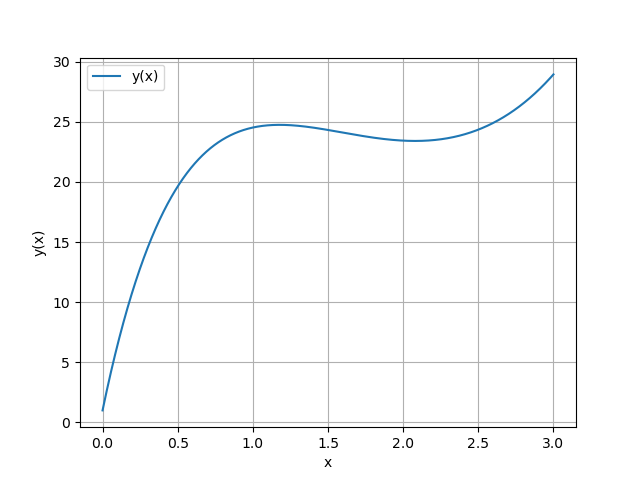
\includegraphics[width=1\linewidth]{2021/CE/26/figures/figure1.png}
        \caption{Plot of y(x)}
    \label{fig:enter-label}
\end{figure}


%\end{document}





\pagebreak
\item A system has a transfer function
\begin{align}
    G(s) = \frac{3e^{-4s}}{12s + 1}\nonumber
\end{align}
When a step-change of magnitude $M$ is given to the system input, the final value of the system output is measured to be 120. The value of M is \_\_\_\_\_.
\hfill(GATE 2021 CH Q52)\\
\solution
\iffalse
\let\negmedspace\undefined
\let\negthickspace\undefined
\documentclass[journal,12pt,twocolumn]{IEEEtran}
\usepackage{cite}
\usepackage{amsmath,amssymb,amsfonts,amsthm}
\usepackage{algorithmic}
\usepackage{graphicx}
\usepackage{textcomp}
\usepackage{xcolor}
\usepackage{txfonts}
\usepackage{listings}
\usepackage{enumitem}
\usepackage{mathtools}
\usepackage{gensymb}
\usepackage{comment}
\usepackage[breaklinks=true]{hyperref}
\usepackage{tkz-euclide} 
\usepackage{listings}
\usepackage{gvv}                            \usepackage{tikz}
\usepackage{circuitikz}
\def\inputGnumericTable{}                                
\usepackage[latin1]{inputenc}                            
\usepackage{color}                                       
\usepackage{array}                                       
\usepackage{longtable}                                   
\usepackage{calc}                              
\usepackage{tikz}
\usepackage{multirow}                                    
\usepackage{hhline}                                      
\usepackage{ifthen}                            
\usepackage{caption}
\usepackage{lscape}
\usepackage{amsmath}
\newtheorem{theorem}{Theorem}[section]
\newtheorem{problem}{Problem}
\newtheorem{proposition}{Proposition}[section]
\newtheorem{lemma}{Lemma}[section]
\newtheorem{corollary}[theorem]{Corollary}
\newtheorem{example}{Example}[section]
\newtheorem{definition}[problem]{Definition}
\newcommand{\BEQA}{\begin{eqnarray}}
\newcommand{\EEQA}{\end{eqnarray}}
\newcommand{\define}{\stackrel{\triangle}{=}}
\theoremstyle{remark}
\newtheorem{rem}{Remark}

\begin{document}

\bibliographystyle{IEEEtran}
\vspace{3cm}

\title{GATE 2021 CH Q52}
\author{EE23BTECH11009 - AROSHISH PRADHAN$^{*}$% <-this % stops a space
}
\maketitle
\newpage
\bigskip
\textbf{Question:} A system has a transfer function
\begin{align}
    G(s) = \frac{3e^{-4s}}{12s + 1}\nonumber
\end{align}
When a step-change of magnitude $M$ is given to the system input, the final value of the system output is measured to be 120. The value of M is \_\_\_\_\_.
\hfill(GATE 2021 CH Q52)\\
\solution
\fi
\begin{table}[!h]
    \centering
    \begin{tabular}{|c|c|c|}
    \hline
       \textbf{Symbol}  & \textbf{Value} & \textbf{Description}\\
    \hline
        $x(t)$ & $Mu(t)$ & Input Signal\\
    \hline
        $X(s)$ & $\frac{M}{s}$ & s-domain Input Signal\\
    \hline
        $y(t)$ &  & Output Signal\\
    \hline
        $Y(s)$ & & s-domain Output Signal\\
    \hline
       $G(s)$ & $\frac{3e^{-4s}}{12s + 1}$ & Transfer Function\\
    \hline
    \end{tabular}
    \caption{Given Parameters}
    \label{tab:1_gate.21.ch.52}
\end{table}


Given, input step-change:
\begin{align}
    x(t) &= Mu(t)\\
    u(t) &\system{L} \frac{1}{s}\\
    \implies X(s) &= \frac{M}{s}
\end{align}
Transfer Function:
\begin{align}
    G(s) &= \frac{Y(s)}{X(s)} = \frac{3e^{-4s}}{12s + 1}\\
    \implies Y(s) &= \frac{3e^{-4s}}{12s + 1}\frac{M}{s}
\end{align}
$\therefore$ system output
\begin{align}
     \lim_{s\rightarrow0}sY(s) &= 120\\
    \implies \lim_{s\rightarrow0}\brak{\frac{3e^{-4s}}{12s + 1}M} &= 120\\
    \implies 3M &= 120\\
    \implies M &= 40
\end{align}

\begin{figure}
    \centering
    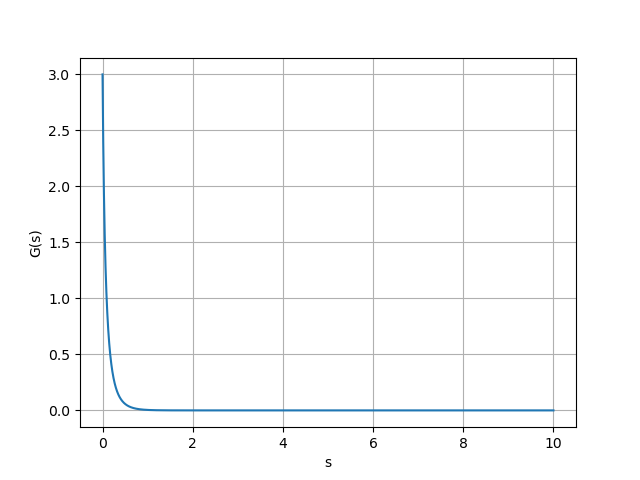
\includegraphics[width = \columnwidth]{2021/CH/52/figs/assign9.png}
	\caption{Plot of $G(s)$ vs $s$}
    \label{fig:1_gate.21.ch.52}
\end{figure}
%\end{document}

\pagebreak
\item The Bode magnitude plot for the transfer function $\frac{V_o(s)}{V_i(s)}$ of the circuit is as shown. The value of R is \_\_\_\_\_$\Omega$. \hfill(GATE 2021 EE Q20)
\begin{figure}[!ht]
    \centering
    \begin{circuitikz}
   \draw(0,0) to [R](2,0);
   % \draw (2,0) -- (2.5,0);
   \draw(2,0) to [L] (4,0);
   % \draw (5,0) to (5,0);
   \draw (4,0) to [C] (4,-2);
   \draw(4,-2)  to (0,-2);
   \draw (4,0) -- (5,0);
   \draw (4,-2)to (5,-2);
   \node[circle,fill,inner sep=1pt] at (0,0) {};
   \node[circle,fill,inner sep=1pt] at (5,0) {};
   \node[circle,fill,inner sep=1pt] at (5,-2) {};
   \node[circle,fill,inner sep=1pt] at (0,-2) {};
   \draw[->](0,-1.85) to (0,-0.15);
   \draw[->](5,-1.85) to (5,-0.15);
   \node at (0.3,-1) {$V_i$};
   \node at (5.5,-1) {$V_o$};

   \node at (1,0.5) {$R$};
   \node at (3,0.5) {$1mH$};
   \node at (2.8,-1) {$250\micro F$};\node[circle,fill,inner sep=1pt] at (0,0) {};
\end{circuitikz}

\end{figure}
\begin{figure}[!ht]
    \centering
    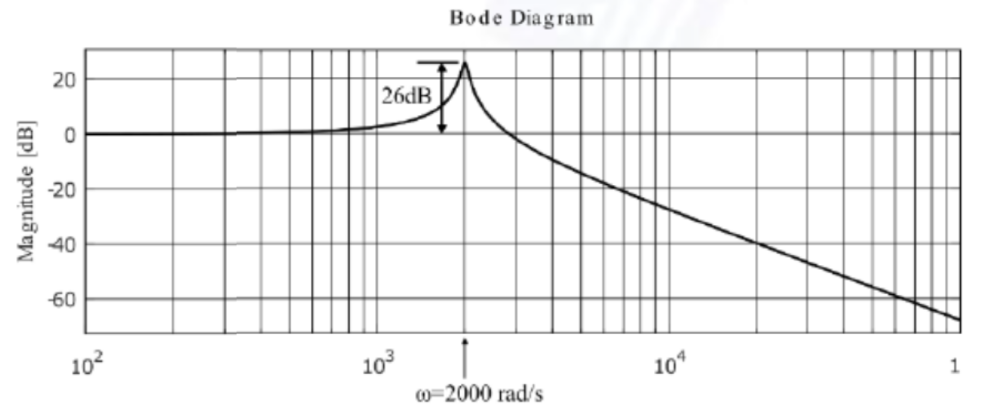
\includegraphics[width=\columnwidth]{2021/EE/20/figs/bode.png}
\end{figure}
\solution
\iffalse
\let\negmedspace\undefined
\let\negthickspace\undefined
\documentclass[journal,12pt,twocolumn]{IEEEtran}
\usepackage{cite}
\usepackage{amsmath,amssymb,amsfonts,amsthm}
\usepackage{algorithmic}
\usepackage{textcomp}
\usepackage{xcolor}
\usepackage{txfonts}
\usepackage{listings}
\usepackage{enumitem}
\usepackage{mathtools}
\usepackage{gensymb}
\usepackage{comment}
\usepackage[breaklinks=true]{hyperref}
\usepackage{tkz-euclide} 
\usepackage{listings}
\usepackage{gvv}                            \usepackage{tikz}
\usepackage{circuitikz}
\def\inputGnumericTable{}                                
\usepackage[latin1]{inputenc}                            
\usepackage{color}                                       
\usepackage{array}                                       
\usepackage{longtable}                                   
\usepackage{calc}                              
\usepackage{tikz}
\usepackage{multirow}                                    
\usepackage{hhline}                                      
\usepackage{ifthen}                            
\usepackage{caption}
\usepackage{lscape}
\usepackage{amsmath}
\newtheorem{theorem}{Theorem}[section]
\newtheorem{problem}{Problem}
\newtheorem{proposition}{Proposition}[section]
\newtheorem{lemma}{Lemma}[section]
\newtheorem{corollary}[theorem]{Corollary}
\newtheorem{example}{Example}[section]
\newtheorem{definition}[problem]{Definition}
\newcommand{\BEQA}{\begin{eqnarray}}
\newcommand{\EEQA}{\end{eqnarray}}
\newcommand{\define}{\stackrel{\triangle}{=}}
\theoremstyle{remark}
\newtheorem{rem}{Remark}

\begin{document}

\bibliographystyle{IEEEtran}
\vspace{3cm}

\title{GATE 2021 EE.20}
\author{EE23BTECH11010 - VENKATESH BANDAWAR$^{*}$% <-this % stops a space
}
\maketitle
\newpage
\bigskip
\textbf{Question:} The Bode magnitude plot for the transfer function $\frac{V_o(s)}{V_i(s)}$ of the circuit is as shown. The value of R is \_\_\_\_\_$\Omega$. \hfill(GATE 2021 EE Q20)
\begin{figure}[!ht]
    \centering
    \begin{circuitikz}
   \draw(0,0) to [R](2,0);
   % \draw (2,0) -- (2.5,0);
   \draw(2,0) to [L] (4,0);
   % \draw (5,0) to (5,0);
   \draw (4,0) to [C] (4,-2);
   \draw(4,-2)  to (0,-2);
   \draw (4,0) -- (5,0);
   \draw (4,-2)to (5,-2);
   \node[circle,fill,inner sep=1pt] at (0,0) {};
   \node[circle,fill,inner sep=1pt] at (5,0) {};
   \node[circle,fill,inner sep=1pt] at (5,-2) {};
   \node[circle,fill,inner sep=1pt] at (0,-2) {};
   \draw[->](0,-1.85) to (0,-0.15);
   \draw[->](5,-1.85) to (5,-0.15);
   \node at (0.3,-1) {$V_i$};
   \node at (5.5,-1) {$V_o$};

   \node at (1,0.5) {$R$};
   \node at (3,0.5) {$1mH$};
   \node at (2.8,-1) {$250\micro F$};\node[circle,fill,inner sep=1pt] at (0,0) {};
\end{circuitikz}

\end{figure}
\begin{figure}[!ht]
    \centering
    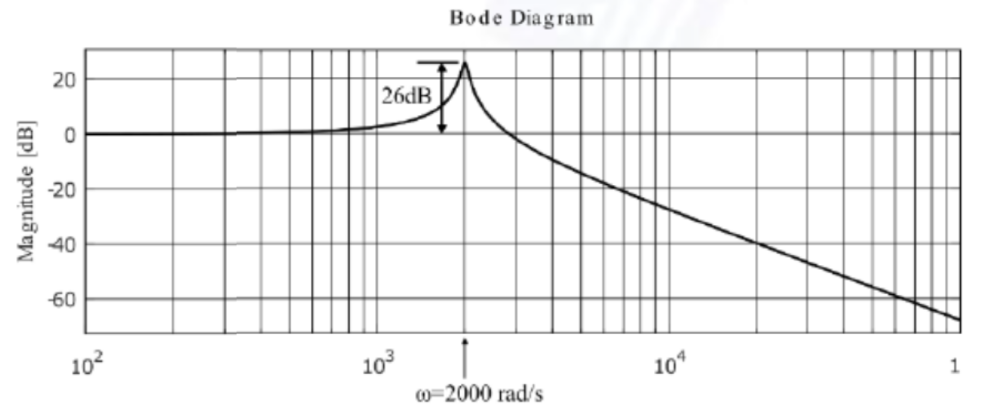
\includegraphics[width=\columnwidth]{2021/EE/20/figs/bode.png}
\end{figure}
\solution
\fi
\begin{table}[!ht]
    \centering
    \begin{tabular}{|c|c|c|}
\hline
    \textbf{Parameter} & \textbf{Description} & \textbf{Value} \\
    \hline
    $C$ & Capacitance & $250\micro F$\\
    \hline
    $L$ & Inductor & $1mH$\\
    \hline
    $I$ & Current &  \\
    \hline
    $I(0)$ & Initial Current & 0A \\
    \hline
    $V_o$ & Voltage across capacitor & \\
    \hline 
    $V_i$ & Input Voltage & \\
    \hline 
    $T(s)$ & Transfer Function & $\frac{V_o(s)}{V_i(s)}$\\
    \hline
    \end{tabular}

    \caption{Given Parameters table}
    \label{Given Parameters table_2021_EE_20}
\end{table}
Applying KVL,
\begin{align}
    V_i - R I - L\frac{dI}{dt} - \frac{\int I dt}{C} = 0
\end{align}
Taking Laplace Transform ,
\begin{align}
    V_i(s) &- RI(s) - LsI(s) + LI(0^+) - \frac{I(s)}{sC} = 0\\
    I(s) &= \frac{V_i(s) + LI(0)}{R + sL + \frac{1}{sC}}\\
    V_o(s) &= \frac{V_i(s) + LI(0)}{RsC + s^2LC + 1}
\end{align}
Substituting $I(0) = 0$ and $s = j\omega$,
\begin{align}
    \frac{V_o(j\omega)}{V_i(j\omega)} &= \frac{1}{\omega RCj -\omega^2LC + 1} 
\end{align}
$\because$ Magnitude in bode plot = $20\log \abs{T(s)}$\\
From given graph,At $\omega = 2000$
\begin{align}
    26 &= 20 \log \abs{\frac{V_o}{V_i}}\\
    \abs{\frac{V_o}{V_i}} &= 20
\end{align}
\begin{align}
    \implies 20 &= \abs{\frac{1}{\omega RCj -\omega^2LC + 1}} \\
    R &= 0.1 \Omega
\end{align}
\begin{figure}[!h]
    \centering
    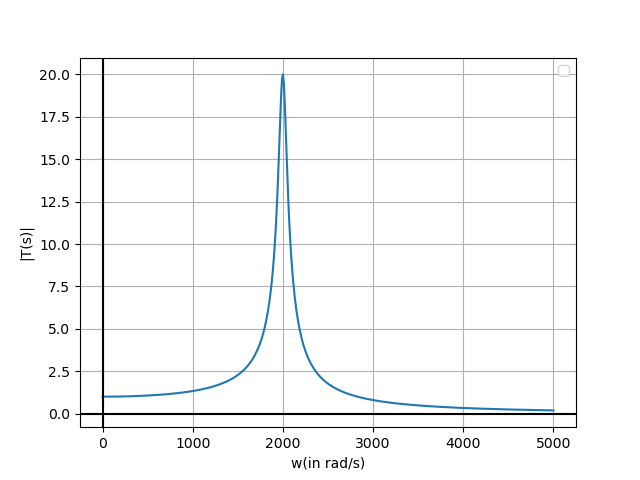
\includegraphics[width=\columnwidth]{2021/EE/20/figs/frequency_response.png}
    \caption{Frequency response of $V_o$}
    \label{frequency_response_2021_EE_20}
\end{figure}
%\end{document}

\pagebreak
\item Consider a system with transfer-function $G\brak{s}=\frac{2}{s+1}$. A unit-step function $\mu\brak{t}$ is applied to the system, which results in an output y\brak{t}. 

If $e\brak{t}=y\brak{t}-\mu\brak{t}$ then $ \lim_{t\to\infty} e(t)$ is\rule{1.5cm}{0.15mm}.
\solution
\iffalse
\let\negmedspace\undefined
\let\negthickspace\undefined
\documentclass[journal,12pt,twocolumn]{IEEEtran}
\usepackage{cite}
\usepackage{amsmath,amssymb,amsfonts,amsthm}
\usepackage{algorithmic}
\usepackage{graphicx}
\usepackage{textcomp}
\usepackage{xcolor}
\usepackage{txfonts}
\usepackage{listings}
\usepackage{enumitem}
\usepackage{mathtools}
\usepackage{gensymb}
\usepackage{comment}
\usepackage[breaklinks=true]{hyperref}
\usepackage{tkz-euclide} 
\usepackage{listings}
\usepackage{gvv}                                        
\def\inputGnumericTable{}                                 
\usepackage[latin1]{inputenc}                                
\usepackage{color}                                            
\usepackage{array}                                            
\usepackage{longtable}                                       
\usepackage{calc}                                             
\usepackage{multirow}                                         
\usepackage{hhline}                                           
\usepackage{ifthen}                                           
\usepackage{lscape}
\newtheorem{theorem}{Theorem}[section]
\newtheorem{problem}{Problem}
\newtheorem{proposition}{Proposition}[section]
\newtheorem{lemma}{Lemma}[section]
\newtheorem{corollary}[theorem]{Corollary}
\newtheorem{example}{Example}[section]
\newtheorem{definition}[problem]{Definition}
\newcommand{\BEQA}{\begin{eqnarray}}
\newcommand{\EEQA}{\end{eqnarray}}
\newcommand{\define}{\stackrel{\triangle}{=}}
\theoremstyle{remark}
\usepackage{circuitikz}
\newtheorem{rem}{Remark}
\begin{document}
\parindent 0px

\bibliographystyle{IEEEtran}
\vspace{3cm}

\title{Assignment\\[1ex]GATE-IN-46}
\author{EE23BTECH11034 - Prabhat Kukunuri$^{}$% <-this % stops a space
}
\maketitle
\newpage
\bigskip

\renewcommand{\thefigure}{\theenumi}
\renewcommand{\thetable}{\theenumi}
\section{Question}
Consider a system with transfer-function $G\brak{s}=\frac{2}{s+1}$. A unit-step function $\mu\brak{t}$ is applied to the system, which results in an output y\brak{t}. 

If $e\brak{t}=y\brak{t}-\mu\brak{t}$ then $ \lim_{t\to\infty} e(t)$ is\rule{1.5cm}{0.15mm}.

\solution
\fi
\begin{table}[h]
    \centering
    \begin{tabular}{|p{1cm}|p{3.00cm}|p{3.50cm}|}
    \hline
    Symbol&Value&Description\\ \hline
    $$G\brak{s}$$&$$\frac{2}{s+1}$$&$$\text{Transfer function}$$\\\hline
    $$e\brak{t}$$&$$y\brak{t}-\mu\brak{t}$$&$$\text{Function of y\brak{t} and $\mu\brak{t}$}$$\\\hline
    $$Y\brak{s}$$&$$G\brak{s}\times U\brak{s}$$&Convolution in $t$ domain is multiplication in $s$ domain.\\\hline
    $$\mu\brak{t}$$&$$\begin{cases}
    0&\text{if t$<$0}\\
    1&\text{if t$>$0}
    \end{cases}$$&$$\text{Unit step function}$$\\\hline
    \end{tabular}
    \caption{Variable description}
    \label{tab:GATE.2021.IN.46.1}
\end{table}\\
Applying Laplace transform on $\mu\brak{t}$
\begin{align}
    &\mu\brak{t}\system{L}U\brak{s}\\
    &U\brak{s}=\frac{1}{s}\\
    &Y\brak{s}=\brak{\frac{2}{s+1}}\brak{\frac{1}{s}}\\
    &Y\brak{s}=\frac{2}{s}-\frac{2}{s+1}
\end{align}
The inverse Laplace transform of $\frac{a}{s+b}$ is $ae^{-bt}\mu\brak{t}$
\begin{align}
    &y\brak{t}=2\mu\brak{t}-2e^{-t}\mu\brak{t}\\
    &e\brak{t}=\mu\brak{t}\brak{1-2e^{-t}}\\
    &\lim_{t\to\infty}e\brak{t}=\lim_{t\to\infty}\mu\brak{t}\brak{1-2e^{-t}}\\
    &\lim_{t\to\infty}e\brak{t}=1
\end{align}
%\end{document}

\end{enumerate}

\chapter{Fourier transform}
\section{2022}
 \begin{enumerate}[label=\thechapter.\arabic*,ref=\thechapter.\theenumi]
\item The outputs of four systems $\brak{S_{1} , S_{2} , S_{3},S_{4}}$ corresponding to the input signal $\sin\brak{t}$, for all time $t$ , are shown in the figure. Based on the given information, which of the four systems is/are definately NOT LTI(linear and time-invariant)? 
\begin{figure}[H]
    \resizebox{0.34\textwidth}{!}{\tikzset{
    block/.style = {draw, fill=white, rectangle, minimum height=3em, minimum width=3em}
}

\begin{tikzpicture}[auto, node distance=2cm,>=Latex]

    \node (input) {$\sin\brak{t}$};
    

    \node [block, right=of input] (s1) {$S_{1}$};
    
    \draw[dashed, draw=black] ($(s1.south west) + (-0.2,-0.2)$) rectangle ($(s1.north east) + (0.2,0.2)$);
    \draw [->] (input) -- (s1);
    \draw [->] (s1) -- ++(2,0) node[right]{$\sin\brak{-t}=-\sin\brak{t}$};
    \begin{scope}[yshift=-3cm]
        \node (input2) {$\sin\brak{t}$};
        \node [block, right=of input2] (s2) {$S_{2}$};
        \draw[dashed, draw=black] ($(s2.south west) + (-0.2,-0.2)$) rectangle ($(s2.north east) + (0.2,0.2)$);
        \draw [->] (input2) -- (s2);
        \draw [->] (s2) -- ++(2,0) node[right]{$\sin\brak{t+1}$};
    \end{scope}
    
    \begin{scope}[yshift=-6cm]
        \node (input3) {$\sin\brak{t}$};
        
   
        \node [block, right=of input3] (s3) {$S_{3}$};
        
   
        \draw[dashed, draw=black] ($(s3.south west) + (-0.2,-0.2)$) rectangle ($(s3.north east) + (0.2,0.2)$);
        

        \draw [->] (input3) -- (s3);
        \draw [->] (s3) -- ++(2,0) node[right]{$\sin\brak{2t}$};
    \end{scope}
       \begin{scope}[yshift=-9cm]
        \node (input3) {$\sin\brak{t}$};
        

        \node [block, right=of input3] (s3) {$S_{4}$};
        

        \draw[dashed, draw=black] ($(s3.south west) + (-0.2,-0.2)$) rectangle ($(s3.north east) + (0.2,0.2)$);
        

        \draw [->] (input3) -- (s3);
        \draw [->] (s3) -- ++(2,0) node[right]{$\sin^2\brak{t}$};
    \end{scope}
\end{tikzpicture}

}
    \caption{Block Diagram of Systems}
    \label{fig:question_fig_EC_Q46}
\end{figure}
\hfill(GATE22 EC Q46)\\
\solution
\iffalse
\let\negmedspace\undefined
\let\negthickspace\undefined
\documentclass[journal,12pt,twocolumn]{IEEEtran}
\usepackage{cite}
\usepackage{amsmath,amssymb,amsfonts,amsthm}
\usepackage{algorithmic}
\usepackage{graphicx}
\usepackage{textcomp}
\usepackage{xcolor}
\usepackage{txfonts}
\usepackage{listings}
\usepackage{enumitem}
\usepackage{mathtools}
\usepackage{float}
\usepackage{gensymb}
\usepackage{comment}
\usepackage[breaklinks=true]{hyperref}
\usepackage{tkz-euclide} 
\usepackage{listings}
\usepackage{gvv}                                        
\def\inputGnumericTable{}                                 
\usepackage[latin1]{inputenc}                                
\usepackage{color}                                            
\usepackage{array}          
\usetikzlibrary{positioning, arrows.meta,shapes}
\usepackage{longtable}                                       
\usepackage{calc}                                             
\usepackage{multirow}                                         
\usepackage{hhline}                                           
\usepackage{ifthen}                                           
\usepackage{lscape}
\usepackage{amsmath}
\newtheorem{theorem}{Theorem}[section]
\newtheorem{problem}{Problem}
\newtheorem{proposition}{Proposition}[section]
\newtheorem{lemma}{Lemma}[section]
\newtheorem{corollary}[theorem]{Corollary}
\newtheorem{example}{Example}[section]
\newtheorem{definition}[problem]{Definition}
\newcommand{\BEQA}{\begin{eqnarray}}
\newcommand{\EEQA}{\end{eqnarray}}
\newcommand{\define}{\stackrel{\triangle}{=}}
\theoremstyle{remark}
\newtheorem{rem}{Remark}
\begin{document}

\bibliographystyle{IEEEtran}
\title{GATE-EC-Q46}
\author{EE23BTECH11015 - DHANUSH V NAYAK$^{*}$% <-this % stops a space
}
\maketitle
\newpage
\bigskip
\renewcommand{\thefigure}{\arabic{figure}}
\renewcommand{\thetable}{\theenumi}
\textbf{Question:} The outputs of four systems $\brak{S_{1} , S_{2} , S_{3},S_{4}}$ corresponding to the input signal $\sin\brak{t}$, for all time $t$ , are shown in the figure. Based on the given information, which of the four systems is/are definately NOT LTI(linear and time-invariant)? 
\begin{figure}[H]
    \resizebox{0.34\textwidth}{!}{\tikzset{
    block/.style = {draw, fill=white, rectangle, minimum height=3em, minimum width=3em}
}

\begin{tikzpicture}[auto, node distance=2cm,>=Latex]

    \node (input) {$\sin\brak{t}$};
    

    \node [block, right=of input] (s1) {$S_{1}$};
    
    \draw[dashed, draw=black] ($(s1.south west) + (-0.2,-0.2)$) rectangle ($(s1.north east) + (0.2,0.2)$);
    \draw [->] (input) -- (s1);
    \draw [->] (s1) -- ++(2,0) node[right]{$\sin\brak{-t}=-\sin\brak{t}$};
    \begin{scope}[yshift=-3cm]
        \node (input2) {$\sin\brak{t}$};
        \node [block, right=of input2] (s2) {$S_{2}$};
        \draw[dashed, draw=black] ($(s2.south west) + (-0.2,-0.2)$) rectangle ($(s2.north east) + (0.2,0.2)$);
        \draw [->] (input2) -- (s2);
        \draw [->] (s2) -- ++(2,0) node[right]{$\sin\brak{t+1}$};
    \end{scope}
    
    \begin{scope}[yshift=-6cm]
        \node (input3) {$\sin\brak{t}$};
        
   
        \node [block, right=of input3] (s3) {$S_{3}$};
        
   
        \draw[dashed, draw=black] ($(s3.south west) + (-0.2,-0.2)$) rectangle ($(s3.north east) + (0.2,0.2)$);
        

        \draw [->] (input3) -- (s3);
        \draw [->] (s3) -- ++(2,0) node[right]{$\sin\brak{2t}$};
    \end{scope}
       \begin{scope}[yshift=-9cm]
        \node (input3) {$\sin\brak{t}$};
        

        \node [block, right=of input3] (s3) {$S_{4}$};
        

        \draw[dashed, draw=black] ($(s3.south west) + (-0.2,-0.2)$) rectangle ($(s3.north east) + (0.2,0.2)$);
        

        \draw [->] (input3) -- (s3);
        \draw [->] (s3) -- ++(2,0) node[right]{$\sin^2\brak{t}$};
    \end{scope}
\end{tikzpicture}

}
    \caption{Block Diagram of Systems}
    \label{fig:question_fig_EC_Q46}
\end{figure}
\hfill(GATE22 EC Q46)\\
\solution 
\fi
\begin{table}[H]
\centering
\renewcommand\thetable{1}
\setlength{\extrarowheight}{9pt}
\resizebox{0.4\textwidth}{!}{
\begin{tabular}{|c|c|c|}
\hline
\textbf{Parameter} & \textbf{Description} \\ \hline
$\brak{S_{1} , S_{2} , S_{3},S_{4}}$ & Systems Given  \\ \hline
$\sin\brak{t}$ & Input \\ \hline
$H\brak{\omega}$ & Transfer Function \\ \hline
$X\brak{\omega}$ & Fourier-Transform of input \\ \hline
$Y\brak{\omega}$ & Fourier-Transform of output \\ \hline
$\Phi(\omega)$ & Phase of Transfer Function \\ \hline
\end{tabular}}
\caption{Parameter Table}
\label{tab:gate_ec_Q46}
\end{table}

\begin{figure}[H]
    \resizebox{0.55\textwidth}{!}{\tikzset{
    block/.style = {draw, fill=white, rectangle, minimum height=3em, minimum width=3em}
}

\begin{tikzpicture}[auto, node distance=2cm,>=Latex]
    \node (input) {$x\brak{t}$};
    \node [block, right=of input] (s1) {$H\brak{\omega}$};
    \draw[dashed, draw=black] ($(s1.south west) + (-0.2,-0.2)$) rectangle ($(s1.north east) + (0.2,0.2)$);
    \draw [->] (input) -- (s1);
    \draw [->] (s1) -- ++(2,0) node[right]{$y\brak{t}$};
    \end{tikzpicture}

    }
    \caption{Block Diagram of LTI System}
    \label{fig:LTI_system_EC_q46}
\end{figure}
For an LTI system :
\begin{align}
    y(t)&=h(t)*x(t)\\
    Y\brak{\omega}&=H\brak{\omega}X\brak{\omega}
\end{align}
$H\brak{\omega}$ is a complex exponential :
\begin{align}
    H(j\omega)=\abs{H(j\omega)}e^{j\Phi\brak{\omega}}
\end{align}
$x(t)=\sin\brak{t}$, and $w_{o}=1 rad/sec$
\begin{align}
    X\brak{\omega}&=j\pi \brak{\delta(\omega+\omega_0)-\delta(\omega-\omega_0)}
\end{align}
Now,

\begin{align}
    Y\brak{\omega}=&\brak{\delta(\omega+\omega_0)-\delta(\omega-\omega_0)}\pi \abs{H\brak{\omega}}e^{j\Phi\brak{\omega}}\label{eq:gate22_ec_q46.1}
\end{align}

\begin{align}
    x\brak{t}\delta\brak{t-t_{o}} = x\brak{t_{0}}\delta\brak{t-t_{o}} \label{eq:gate_22_ec_delta_prop_1}
\end{align}
Using property \eqref{eq:gate_22_ec_delta_prop_1} in \eqref{eq:gate22_ec_q46.1} :
\begin{align}
    Y\brak{\omega}=&j\pi \abs{H(-\omega_0)}e^{j\Phi(-\omega_0)}\delta(\omega+\omega_0)\label{eq:gate_ec_q46.3} \\&- j\pi \abs{H\brak{\omega_0}}e^{j\Phi(j\omega_0)}\delta(\omega-\omega_0) \notag 
\end{align}
By definition of the Fourier transform,
\begin{align}
    X(\omega) &= \int_{-\infty}^{\infty} x\brak{t}e^{-j\omega t} \,dt \\
    X^*(\omega) &= \int_{-\infty}^{\infty} x^*(t)e^{j\omega t} \,dt \\
    X^*(-\omega) &= \int_{-\infty}^{\infty} x^*(t)e^{-j\omega t} \,dt\label{eq:gate_ec_q46.2}
\end{align}
For real-time domain signal :
\begin{align}
    x\brak{t} &= x^*\brak{t}
\end{align}
Therefore , from \eqref{eq:gate_ec_q46.2}:
\begin{align}
    X(\omega) =  X^*(-\omega) \label{eq:gate_ec_q46_conjsymm}
\end{align}
By \eqref{eq:gate_ec_q46_conjsymm} , Given $h(t)$ a real-time domain signal, $H\brak{\omega}$ is conjugate symmetric.
\begin{align}
    \abs{H\brak{\omega}}=\abs{H(-\omega)}\label{eq:gate_22_q46_conj_result1}\\
    \Phi(-\omega)=-\Phi\brak{\omega}\label{eq:gate_22_q46_conj_result2}
\end{align}
Therefore using \eqref{eq:gate_22_q46_conj_result1} and \eqref{eq:gate_22_q46_conj_result2} in \eqref{eq:gate_ec_q46.3},
 \begin{align}
    Y\brak{\omega}= j\pi \abs{H\brak{\omega_0}}\brak{e^{-j\Phi\brak{\omega_0}}\delta(\omega+\omega_0) - e^{j\Phi\brak{\omega_0}}\delta(\omega-\omega_0)}
\end{align}
Taking Inverse Fourier Transform, 
\begin{align}
    &\delta(\omega-\omega_0) \system{F} \frac{1}{2\pi}e^{j\omega_0t}\\
     &\delta(\omega+\omega_0) \system{F} \frac{1}{2\pi}e^{-j\omega_0t}\\
    &\implies y(t)=j\abs{H\brak{\omega_0}}\frac{1}{2}\brak{e^{-j\brak{\omega_0t+\Phi\brak{\omega_0}}}-e^{j\brak{\omega_0t+\Phi\brak{\omega_0}}}}\\
    &\implies y(t) =\abs{H\brak{\omega_0}}\sin{\brak{\omega_0t+\Phi\brak{\omega_0}}} 
\end{align}
$w_{0} = 1$ rad/sec :
\begin{align}
    y(t) =\abs{H\brak{1}}\sin{\brak{t+\Phi\brak{1}}} \label{eq:gate_ec_q46_finaloutput}
\end{align}
From \eqref{eq:gate_ec_q46_finaloutput} we can see output cant have scaled frequency nor a squared output. But can have a shifted output or amplitude-scaled output. \\

So, $S_{3}$ and $S_{4}$ cannot be LTI system.
%\end{document}


\pagebreak

    \item The Fourier transform X\brak{j\omega} of the signal\\ $x(t)=\frac{t}{\brak{1+t^2}^2}$ is \rule{1.5cm}{0.15mm}.\hfill{GATE-2022-EC-15}
\begin{enumerate}
	\item[(A)] $\frac{\pi}{2j}\omega e^{-\abs{\omega}}$
	\item[(B)] $\frac{\pi}{2}\omega e^{-\abs{\omega}}$
	\item[(C)] $\frac{\pi}{2j}e^{-\abs{\omega}}$
	\item[(D)] $\frac{\pi}{2}e^{-\abs{\omega}}$
\end{enumerate}

\solution
% \iffalse
\let\negmedspace\undefined
\let\negthickspace\undefined
\documentclass[journal,12pt,twocolumn]{IEEEtran}
\usepackage{cite}
\usepackage{amsmath,amssymb,amsfonts,amsthm}
\usepackage{algorithmic}
\usepackage{graphicx}
\usepackage{textcomp}
\usepackage{xcolor}
\usepackage{txfonts}
\usepackage{listings}
\usepackage{enumitem}
\usepackage{mathtools}
\usepackage{gensymb}
\usepackage{comment}
\usepackage[breaklinks=true]{hyperref}
\usepackage{tkz-euclide} 
\usepackage{listings}
\usepackage{gvv}                                        
\def\inputGnumericTable{}                                 
\usepackage[latin1]{inputenc}                                
\usepackage{color}                                            
\usepackage{array}                                            
\usepackage{longtable}                                       
\usepackage{calc}                                             
\usepackage{multirow}                                         
\usepackage{hhline}                                           
\usepackage{ifthen}                                           
\usepackage{lscape}

\makeatletter

\newcommand*{\underarrow}{\def\@underarrow{\relax}\@ifstar{\@@underarrow}{\def\@underarrow{\hidewidth}\@@underarrow}}
\newcommand*{\@@underarrow}[2][]{\underset{\@underarrow\substack{\uparrow\if\relax\detokenize{#1}\relax\else\\#1\fi}\@underarrow}{#2}}

\newcommand*{\overarrow}{\def\@overarrow{\relax}\@ifstar{\@@overarrow}{\def\@overarrow{\hidewidth}\@@overarrow}}
\newcommand*{\@@overarrow}[2][]{\overset{\@overarrow\substack{\if\relax\detokenize{#1}\relax\else#1\\\fi\downarrow}\@overarrow}{#2}}
\makeatother
\newtheorem{theorem}{Theorem}[section]
\newtheorem{problem}{Problem}
\newtheorem{proposition}{Proposition}[section]
\newtheorem{lemma}{Lemma}[section]
\newtheorem{corollary}[theorem]{Corollary}
\newtheorem{example}{Example}[section]
\newtheorem{definition}[problem]{Definition}
\newcommand{\BEQA}{\begin{eqnarray}}
\newcommand{\EEQA}{\end{eqnarray}}
\newcommand{\define}{\stackrel{\triangle}{=}}
\theoremstyle{remark}
\newtheorem{rem}{Remark}
\begin{document}
\parindent 0px

\bibliographystyle{IEEEtran}
\vspace{3cm}

\title{Assignment\\[1ex]GATE-EE-50}
\author{EE23BTECH11034 - Prabhat Kukunuri$^{}$% <-this % stops a space
}
\maketitle
\newpage
\bigskip

\renewcommand{\thefigure}{\theenumi}
\renewcommand{\thetable}{\theenumi}
\section{Question}
The Fourier transform X\brak{j\omega} of the signal\\ $x(t)=\frac{t}{\brak{1+t^2}^2}$ is \rule{1.5cm}{0.15mm}.
\begin{enumerate}
	\item[(A)] $\frac{\pi}{2j}\omega e^{-\abs{\omega}}$
	\item[(B)] $\frac{\pi}{2}\omega e^{-\abs{\omega}}$
	\item[(C)] $\frac{\pi}{2j}e^{-\abs{\omega}}$
	\item[(D)] $\frac{\pi}{2}e^{-\abs{\omega}}$
\end{enumerate}
\solution
\begin{table}[h]
    \centering
    \begin{tabular}{|p{2cm}|p{2.80cm}|p{2.70cm}|}
    \hline
    Symbol&Value&Description\\ \hline
    $$x(t)$$&$$\frac{t}{\brak{1+t^2}^2}$$&$$\text{Signal}$$\\\hline
    $$X\brak{\omega}$$&$$\int_{t=-\infty}^{\infty}x\brak{t}e^{-j\omega t}dt$$& Fourier transform of $x\brak{t}$\\\hline
    \end{tabular}
    \caption{Variable description}
    \label{tab:GATE-2022-15-1}
\end{table}\\
The Fourier transform of the form x\brak{t}=$e^{-a\abs{t}}$ is 
\begin{align}
    x\brak{t}&\xleftrightarrow{\text{F.T}} X\brak{\omega}\\
    X\brak{\omega}&= \frac{2a}{a^2+\omega^2}
\end{align}
Consider, 
\begin{align}
    x\brak{t}&=e^{-\abs{t}}\\
    X\brak{\omega}&=\frac{2}{1+\omega^2}
\end{align}
By using differentiation property from \eqref{eq:Differentiation-property},
\begin{align}
    tx\brak{t}&\xleftrightarrow{\text{F.T}}j\frac{d}{d\omega}X\brak{\omega}\\
     tx\brak{t}&\xleftrightarrow{\text{F.T}}j\sbrak{\frac{d}{d\omega}\brak{\frac{2}{1+\omega^2}}}\\
     te^{-\abs{t}}&\xleftrightarrow{\text{F.T}}\frac{-4j\omega}{\brak{1+\omega^2}^2}
\end{align}
Applying duality property from \eqref{eq:Duality-property},
\begin{align}
    \frac{-4jt}{\brak{1+t^2}^2}&\xleftrightarrow{\text{F.T}}2\pi\brak{-\omega}e^{-\abs{-\omega}}\\
    \frac{t}{\brak{1+t^2}^2}&\xleftrightarrow{\text{F.T}}\frac{-2\pi\omega e^{-\abs{\omega}}}{-4j}\\
    \frac{t}{\brak{1+t^2}^2}&\xleftrightarrow{\text{F.T}}\frac{\pi}{2j}\omega e^{-\abs{\omega}}
\end{align}
\end{document}

\pagebreak

\item For a vector $\bar{x} = [x[0], x[1], \dots, x[7] ]$, the $8$-point discrete Fourier transform (DFT) is denoted by $\bar{X} = \text{DFT}(\bar{x}) = [X[0],X[1],\dots,X[7]]$, where
    \begin{align*}
    X[k] = \sum_{n=0}^{7}x[n]\exp\left(-j\frac{2\pi}{8}nk\right).
    \end{align*} 
    Here $j = \sqrt{-1}$. If $\bar{x} = [1,0,0,0,2,0,0,0]$ and $\bar{y} = \text{DFT}(\text{DFT}(\bar{x}))$, then the value of $y[0]$ is.\hfill{GATE-2022-EC-55}\\
    \solution
    \iffalse
\documentclass[journal,12pt,onecolumn]{IEEEtran}
\usepackage{cite}
\usepackage{amsmath,amssymb,amsfonts,amsthm}
\usepackage{algorithmic}
\usepackage{graphicx}
\usepackage{textcomp}
\usepackage{xcolor}
\usepackage{txfonts}
\usepackage{listings}
\usepackage{enumitem}
\usepackage{mathtools}
\usepackage{gensymb}
\usepackage{comment}
\usepackage[breaklinks=true]{hyperref}
\usepackage{tkz-euclide}
\usepackage{listings}
\usepackage{gvv}
\def\inputGnumericTable{}
\usepackage[latin1]{inputenc}
\usepackage{color}
\usepackage{array}
\usepackage{longtable}
\usepackage{calc}
\usepackage{multirow}
\usepackage{hhline}
\usepackage{ifthen}
\usepackage{lscape}

\newtheorem{theorem}{Theorem}[section]
\newtheorem{problem}{Problem}
\newtheorem{proposition}{Proposition}[section]
\newtheorem{lemma}{Lemma}[section]
\newtheorem{corollary}[theorem]{Corollary}
\newtheorem{example}{Example}[section]
\newtheorem{definition}[problem]{Definition}
\newcommand{\BEQA}{\begin{eqnarray}}
    \newcommand{\EEQA}{\end{eqnarray}}
\newcommand{\define}{\stackrel{\triangle}{=}}
\theoremstyle{remark}
\newtheorem{rem}{Remark}

\begin{document}
    
    \bibliographystyle{IEEEtran}
    \vspace{3cm}
    
    \title{Gate 2022 EC Q55}
    \author{EE23BTECH11212 - Manugunta Meghana Sai$^{*}$% <-this % stops a space
    }
    \maketitle
    \bigskip
    
    \renewcommand{\thefigure}{\theenumi}
    \renewcommand{\thetable}{\theenumi}
    
    \vspace{3cm}
    \textbf{Gate 2022 EE Q55} 
    
    For a vector $\bar{x} = [x[0], x[1], \dots, x[7] ]$, the $8$-point discrete Fourier transform (DFT) is denoted by $\bar{X} = \text{DFT}(\bar{x}) = [X[0],X[1],\dots,X[7]]$, where
    \begin{align*}
    X[k] = \sum_{n=0}^{7}x[n]\exp\left(-j\frac{2\pi}{8}nk\right).
    \end{align*} 
    Here $j = \sqrt{-1}$. If $\bar{x} = [1,0,0,0,2,0,0,0]$ and $\bar{y} = \text{DFT}(\text{DFT}(\bar{x}))$, then the value of $y[0]$ is\\
    \solution
    \fi
    \begin{table}[h!]
 	\centering
 	\resizebox{6 cm}{!}{
 		\begin{tabular}{|c|c|c|}
	\hline
	\textbf{Parameter} &  \textbf{Description} & \textbf{Value}\\[6pt]
	\hline
	$\bar{X}$ & $\text{DFT}(\bar{x})$ & $-$ \\[6pt]
	\hline
	$\bar{x}$ & vector & $[1,0,0,0,2,0,0,0]$ \\[6pt]
	\hline
	$\bar{y}$ & $\text{DFT}(\text{DFT}(\bar{x}))$ & $-$ \\[6pt]
	\hline 
\end{tabular}

 	}
 	\caption{Given Parameters}
 	\label{tab:msmECgate55tab1} 
 \end{table} 
    \\DFT of $\bar{x}$
    \begin{align}
    X[k] = \sum_{n=0}^{7}x[n]\exp\left(-j\frac{2\pi}{8}nk\right)
    \end{align}
    As the only non-zero values in x are x[0] and x[4]:
    \begin{align}
    X[k] = x[0] + x[4]\exp\left(-j\pi k\right)
    \end{align}
    After substituting the values of k ranging from $0$ to $7$,
    \begin{align}
    \bar{X} &= \text{DFT}(\bar{x}) = [X[0],X[1],\dots,X[7]]\\
    \bar{X} &= [3,-1,3,-1,3,-1,3,-1]
    \end{align}
    \begin{align}
    \bar{y} &= \text{DFT}(\text{DFT}(\bar{x}))\\
    \bar{y} &= [3,-1,3,-1,3,-1,3,-1]\\
    y[0] &= \sum_{n=0}^{7}x[n]\\
    &= x[0] + x[1] + \dots + x[7]\\
    &= 3 -1 +3 -1 +3 -1 +3 -1 = 8
    \end{align}
%\end{document}


    \pagebreak
\item \textbf{Question:} An LTI system is shown in the figure where $$H\brak{s}= \frac{100}{s^2+0.1s+10}$$ The steady state output of the system for an input $x\brak{t}$ is given by $y\brak{t}=a+b\sin{\brak{10t+\theta}}$. The values of $'a'$ and $'b'$ are \\\\
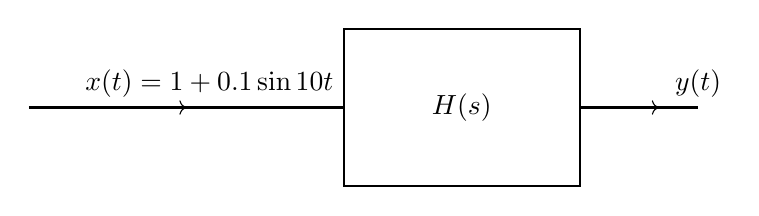
\begin{tikzpicture}
    \draw [thick, draw=black] (-2,-1) -- (2,-1) node[anchor=south east] {$x(t)=1+0.1\sin{\brak{10t}}$};
    \draw [thick,draw=black] (2,0) rectangle (5,-2) ;
    \draw [thick,draw=black] (5,-1) -- (6.5,-1) node[anchor=south] {$y(t)$};
    \draw [->] (-2,-1)--(0,-1);
    \draw [->] (5,-1)--(6,-1);
    \draw (3.5, -1) node[] {$H(s)$};
\end{tikzpicture}\\
\solution 
    \iffalse
\let\negmedspace\undefined
\let\negthickspace\undefined
\documentclass[journal,12pt,twocolumn]{IEEEtran}
\usepackage{cite}
\usepackage{amsmath,amssymb,amsfonts,amsthm}
\usepackage{algorithmic}
\usepackage{graphicx}
\usepackage{textcomp}
\usepackage{xcolor}
\usepackage{txfonts}
\usepackage{listings}
\usepackage{enumitem}
\usepackage{mathtools}
\usepackage{gensymb}
\usepackage{comment}
\usepackage[breaklinks=true]{hyperref}
\usepackage{tkz-euclide} 
\usepackage{listings}
\usepackage{gvv}                                        
%\def\inputGnumericTable{}                                 
\usepackage[latin1]{inputenc}                                
\usepackage{color}                                            
\usepackage{array}                                            
\usepackage{longtable}                                       
\usepackage{calc}                                             
\usepackage{multirow}                                         
\usepackage{hhline}                                           
\usepackage{ifthen}                                           
\usepackage{lscape}
\usepackage{tabularx}
\usepackage{array}
\usepackage{float}


\newtheorem{theorem}{Theorem}[section]
\newtheorem{problem}{Problem}
\newtheorem{proposition}{Proposition}[section]
\newtheorem{lemma}{Lemma}[section]
\newtheorem{corollary}[theorem]{Corollary}
\newtheorem{example}{Example}[section]
\newtheorem{definition}[problem]{Definition}
\newcommand{\BEQA}{\begin{eqnarray}}
\newcommand{\EEQA}{\end{eqnarray}}
\newcommand{\define}{\stackrel{\triangle}{=}}
\theoremstyle{remark}
\newtheorem{rem}{Remark}
\begin{document}

\bibliographystyle{IEEEtran}
\vspace{3cm}

\title{Question 37, EE Gate 2022}
\author{EE23BTECH11017 - Eachempati Mihir Divyansh$^{*}$}
\maketitle
\newpage
\bigskip

\renewcommand{\thefigure}{\theenumi}
\renewcommand{\thetable}{\theenumi}
\textbf{Question:} An LTI system is shown in the figure where $$H\brak{s}= \frac{100}{s^2+0.1s+10}$$ The steady state output of the system for an input $x\brak{t}$ is given by $y\brak{t}=a+b\sin{\brak{10t+\theta}}$. The values of $'a'$ and $'b'$ are \\\\
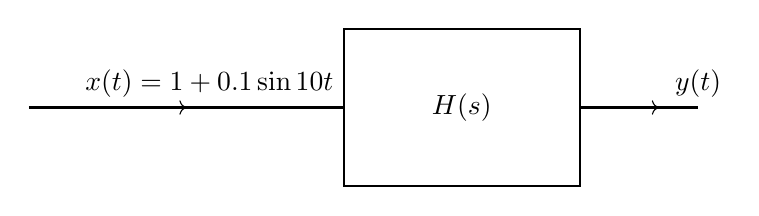
\begin{tikzpicture}
    \draw [thick, draw=black] (-2,-1) -- (2,-1) node[anchor=south east] {$x(t)=1+0.1\sin{\brak{10t}}$};
    \draw [thick,draw=black] (2,0) rectangle (5,-2) ;
    \draw [thick,draw=black] (5,-1) -- (6.5,-1) node[anchor=south] {$y(t)$};
    \draw [->] (-2,-1)--(0,-1);
    \draw [->] (5,-1)--(6,-1);
    \draw (3.5, -1) node[] {$H(s)$};
\end{tikzpicture}

\solution \\
\fi
\begin{table}[h]
    \centering
    \begin{tabular}{|c|c|c|}
    \hline
   Symbol & Value & Description \\
    \hline
    $x\brak{t}$ & $1+0.1\sin{\brak{10t}}$ & Input Signal\\ [2ex]
    \hline
    $y\brak{t}$ & ? & Output of the system\\[2ex]
    \hline 
    $H\brak{s}$ & $\frac{100}{s^2+0.1s+10}$ & Impulse Response\\[2ex]
    \hline
\end{tabular}
    \caption{Given Information} 
    \label{37.Gate22.EE.tab: 1}                                                                                                                                                                                                 
\end{table}
\begin{enumerate}
\item \textbf{Theory: } If a sinusoidal input is given to a system, whose transfer function is known, the output can be calculated as follows
\begin{align}
    y(t)&=h(t)*x(t)\\
    Y(s)&=H(s)X(s)
\end{align}
Let $s=j\omega$
\begin{align}
    Y(j\omega)&=H(j\omega)X(j\omega)
\end{align}
If $\Phi$ is the phase of $H(j\omega)$, 
\begin{align}
    H(j\omega)=\abs{H(j\omega)}e^{j\Phi(\omega)}
\end{align}
If $x(t)=\cos{(\omega_0t)}$, 
\begin{align}
    X(j\omega)&=\pi \brak{\delta(\omega-\omega_0)+\delta(\omega+\omega_0)}
   % \implies X(f)&=\frac{1}{2}\brak{\delta(f-f_0)+\delta(f+f_0)}
\end{align}
Now,
\begin{align}
    Y(j\omega)=&\brak{\delta(\omega-\omega_0)+\delta(\omega+\omega_0)}\abs{H(j\omega)}e^{j\Phi(\omega)}\\
\end{align}
Since $\abs{H(j\omega)}\delta(\omega-\omega_0)$ is zero everywhere except at $\omega_0$ 
\begin{align}
    Y(j\omega)=&\abs{H(j\omega_0)}e^{j\Phi(\omega_0)}\delta(\omega-\omega_0) \\&+ \abs{H(-j\omega_0)}e^{j\Phi(-j\omega_0)}\delta(\omega+\omega_0)
\end{align}
As $h(t)$ is real, $${H(\omega)}={H^{*}(-\omega)}$$ 
 $$\Phi(-\omega_0)=-\Phi(\omega_0)$$
Hence 
 \begin{align}
    Y(\omega)= \abs{H(\omega_0)}\brak{e^{j\Phi(\omega_0)}\delta(\omega-\omega_0) + e^{-j\Phi(\omega_0)}\delta(\omega+\omega_0)}
\end{align}
Taking Inverse Fourier Transform, 
\begin{align}
    &\delta(\omega-\omega_0) \system{F} \frac{1}{2}e^{j\omega_0t}\\
    &\implies y(t)=\abs{H(\omega_0)}\frac{1}{2}\brak{e^{j\brak{\omega_0t+\Phi(\omega_0)}}+e^{-j\brak{\omega_0t+\Phi(\omega_0)}}}\\
    &\implies y(t) = \abs{H(\omega_0)}\cos{\brak{\omega_0t+\Phi(\omega_0)}}
\end{align}
\item The given input can be assumed to be a superposition of $u(t)$ and $0.1\sin{\brak{\omega_0t}}u(t)$. $$\omega_0=0 \text{ and }\omega_0=10$$ for the constant input and the sinusoidal input respectively.
\begin{align}
    y(t)=\abs{H(0)}+\abs{H(10)}\sin{\brak{10t+\Phi(10)}}
\end{align}
Here
\begin{align}
    H(\omega)&=\frac{100}{(j\omega)^2+0.1(j\omega)+10}\\
    \implies H(\omega)&=\frac{100}{10-\omega^2+j(0.1\omega)}\\
    \implies \abs{H(\omega)}&=\frac{100}{\sqrt{(10-\omega^2)^2+(0.1\omega)^2}}\\
    \therefore \abs{H(0)}&=10 \text{ and } \abs{H(10)}\approx 1
\end{align}
The phase $\Phi(\omega)$ is given by 
\begin{align}
    \Phi(\omega)&=\tan^{-1}\frac{0.1\omega}{\omega^2-10}\\
    \implies \Phi(10)&=\tan^{-1} \frac{1}{90}
\end{align}
Hence the output of the system 
\begin{align}
    y(t)=10+\sin{(10t+\tan^{-1} \frac{1}{90})}
\end{align}
Hence $a=10$ and $b=1$ 
\begin{figure}[h]
    \centering
    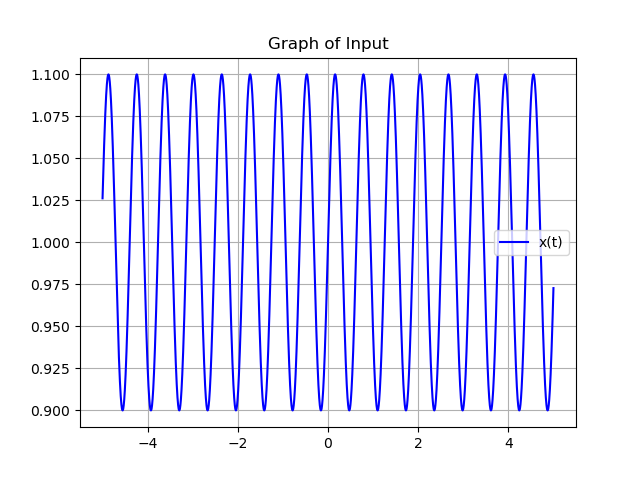
\includegraphics[width=\columnwidth]{2022/EE/37/figs/input.png}
    \caption{Input of the system, $x(t)$} 
\end{figure}
\begin{figure}[h]
    \centering
    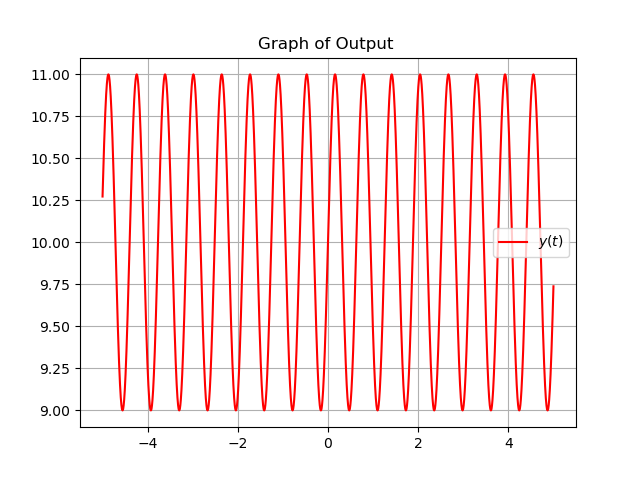
\includegraphics[width=\columnwidth]{2022/EE/37/figs/output.png}
    \caption{Output of the system, $y(t)$} 
\end{figure}
\begin{figure}[h]
    \centering
    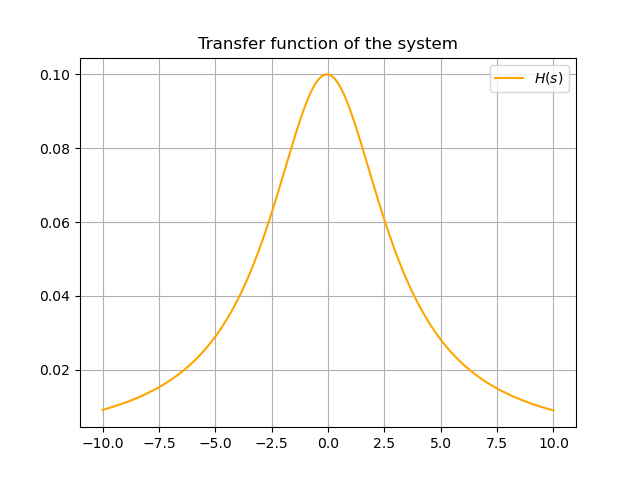
\includegraphics[width=\columnwidth]{2022/EE/37/figs/transfer.png}
    \caption{Transfer function of the system, $H(s)$} 
\end{figure}
% Properties of Laplace transform include 
% \begin{align}
%     ku\brak{t} &\system{L} \frac{k}{s}\label{37.Gate22.EE.eqn: 1}\\  
%     y\brak{t-k} & \system{L} e^{-sk} Y\brak{s} \label{37.Gate22.EE.eqn: 2}\\
%     \sin{\brak{\omega t}} &\system{L} \frac{\omega}{\omega^2 + s^2} \label{37.Gate22.EE.eqn: 3}
% \end{align}
% Taking Laplace transform of $x\brak{t}$, from \eqref{37.Gate22.EE.eqn: 1}, \eqref{37.Gate22.EE.eqn: 2} and \eqref{37.Gate22.EE.eqn: 3}
% \begin{align}
%     %a+b \sin{\brak{10t+\theta}} \system{L} 
%     1+0.1 \sin{\brak{10t}} &\system{L} \frac{1}{s} + 0.1 \frac{10}{s^2+10^2}\\
%  %   &\system{L} \frac{s^2+s+100}{s^2+100}\\
%     \implies X\brak{s} &= \frac{s^2+s+100}{s\brak{s^2+100}} \label{37.Gate22.EE.eqn: 5}
% \end{align}
% From \tabref{37.Gate22.EE.tab: 1},
% \begin{align}
%     G\brak{s}= \frac{Y\brak{s}}{X\brak{s}}=\frac{100}{s^2+0.1s+10} \\
%     \implies Y\brak{s}=X\brak{s} \brak{ \frac{100}{s^2+0.1s+10}}
% \end{align}
% From \eqref{37.Gate22.EE.eqn: 5}
% \begin{align}
%     Y\brak{s}= \frac{s^2+s+100}{s\brak{s^2+100}} \frac{100}{s^2+0.1s+10}\\
%     Y\brak{s}= 100 
% \end{align}
% Consider 
% \begin{align}
%     x(t) = x_1(t)+x_2(t)
% \end{align}
% where $x_1(t)=u(t)$ and $x_2(t)=0.1\sin{(10t)}u(t)$. 
% Since the given system is linear, 
% \begin{align}
%     y(t)=y_1(t)+y_2(t)
% \end{align}
% Where $y_1(t)$ and $y_2(t)$ are the outputs to $x_1(t)$ and $x_2(t)$ respectively.
% \begin{align}
%     y(t) \system{L} Y(s)\\
%     Y_1(s)=G(s)X_1(s)\\
%     Y_1(s)=\frac{1}{s}\brak{\frac{100}{s^2+0.1s+10}} 
% \end{align}
% By partial fractions 
% \begin{align}
%     Y_1(s)=
% \end{align}
% Consider 
% \begin{align}
%     G(s)&\system{L^{-0}}g(t)\\
%     G(s)&=\frac{100}{s^2+0.1s+10}\\
%     &=\frac{100}{(s^+0.05)^2 + 10 - (0.05)^2}\\
% \end{align}
% Let $\brak{10-\brak{0.05}^2}=a^2$ 
% \begin{align}
%     G(s)&=\frac{100}{a}\frac{a}{(s+0.05)^2+a^2}
% \end{align}
% From \eqref{37.Gate22.EE.eqn: 1}, \eqref{37.Gate22.EE.eqn: 2} and \eqref{37.Gate22.EE.eqn: 3}
% \begin{align}
%     g(t)=\frac{100}{a} e^{-0.05t}\sin{(at)}u(t)
% \end{align}
% The output of the system $y(t)$ is given by $$y(t)=x(t)*h(t)$$
% \begin{align}
%     y(t)=&\int_{-\infty}^{\infty} g(u)x(t-u) du\\
%     =&\int_{0}^{\infty} \frac{100}{a} e^{-0.05u}\sin{(au)}du \\&+ \int_{0}^{\infty} \frac{100}{a} e^{-0.05u}\sin{(au)}(0.1\sin{10(t-u)})\\
%     =&\brak{\frac{100}{a}\frac{e^{-0.05u}}{(-0.05)^2+a^2}\brak{(-0.05)\sin{au}-a\cos{au}}}_0^{\infty}\\
%     &+\int_{0}^{\infty} \frac{100}{a} e^{-0.05u}\sin{(au)}(0.1\sin{10(t-u)})\\
%     &=\frac{100}{a^2+(0.05)^2}+
% \end{align}
\end{enumerate}

 

\item A periodic function $f(x)$, with period 2, is defined as \\
   \begin{align}   
   f(x) =
   \begin{cases}
    -1-x & -1 \leq x<0 \\
     1-x &  0 <x \leq1 
   \end{cases}
   \end{align} 
   The Fourier series of this function contains \\
\begin{enumerate}[label=\Alph*.]
\item Both $\cos(n\pi x)$ and $sin(n\pi x)$ where n=1,2,3...
\item Only $\sin(n\pi x)$ where n=1,2,3...
\item Only $\cos(n\pi x)$ where n=1,2,3...
\item Only $\cos(2n\pi x)$ where n=1,2,3...  \hfill{GATE IN 2022 }
\end{enumerate} 

\solution
\let\negmedspace\undefined
\let\negthickspace\undefined
\documentclass[journal,12pt,onecolumn]{IEEEtran}
\usepackage{cite}
\usepackage{amsmath,amssymb,amsfonts,amsthm}
\usepackage{algorithmic}
\usepackage{graphicx}
\usepackage{textcomp}
\usepackage{xcolor}
\usepackage{txfonts}
\usepackage{listings}
\usepackage{enumitem}
\usepackage{mathtools}
\usepackage{gensymb}
\usepackage[breaklinks=true]{hyperref}
\usepackage{tkz-euclide} % loads  TikZ and tkz-base
\usepackage{listings}



\newtheorem{theorem}{Theorem}[section]
\newtheorem{problem}{Problem}
\newtheorem{proposition}{Proposition}[section]
\newtheorem{lemma}{Lemma}[section]
\newtheorem{corollary}[theorem]{Corollary}
\newtheorem{example}{Example}[section]
\newtheorem{definition}[problem]{Definition}
%\newtheorem{thm}{Theorem}[section] 
%\newtheorem{defn}[thm]{Definition}
%\newtheorem{algorithm}{Algorithm}[section]
%\newtheorem{cor}{Corollary}
\newcommand{\BEQA}{\begin{eqnarray}}
\newcommand{\EEQA}{\end{eqnarray}}
\newcommand{\define}{\stackrel{\triangle}{=}}
\theoremstyle{remark}
\newtheorem{rem}{Remark}
%\bibliographystyle{ieeetr}
\begin{document}
%
\providecommand{\pr}[1]{\ensuremath{\Pr\left(#1\right)}}
\providecommand{\prt}[2]{\ensuremath{p_{#1}^{\left(#2\right)} }}        % own macro for this question
\providecommand{\qfunc}[1]{\ensuremath{Q\left(#1\right)}}
\providecommand{\sbrak}[1]{\ensuremath{{}\left[#1\right]}}
\providecommand{\lsbrak}[1]{\ensuremath{{}\left[#1\right.}}
\providecommand{\rsbrak}[1]{\ensuremath{{}\left.#1\right]}}
\providecommand{\brak}[1]{\ensuremath{\left(#1\right)}}
\providecommand{\lbrak}[1]{\ensuremath{\left(#1\right.}}
\providecommand{\rbrak}[1]{\ensuremath{\left.#1\right)}}
\providecommand{\cbrak}[1]{\ensuremath{\left\{#1\right\}}}
\providecommand{\lcbrak}[1]{\ensuremath{\left\{#1\right.}}
\providecommand{\rcbrak}[1]{\ensuremath{\left.#1\right\}}}
\newcommand{\sgn}{\mathop{\mathrm{sgn}}}
\providecommand{\abs}[1]{\left\vert#1\right\vert}
\providecommand{\res}[1]{\Res\displaylimits_{#1}} 
\providecommand{\norm}[1]{\left\lVert#1\right\rVert}
%\providecommand{\norm}[1]{\lVert#1\rVert}
\providecommand{\mtx}[1]{\mathbf{#1}}
\providecommand{\mean}[1]{E\left[ #1 \right]}
\providecommand{\cond}[2]{#1\middle|#2}
\providecommand{\fourier}{\overset{\mathcal{F}}{ \rightleftharpoons}}
\newenvironment{amatrix}[1]{%
  \left(\begin{array}{@{}*{#1}{c}|c@{}}
}{%
  \end{array}\right)
}
%\providecommand{\hilbert}{\overset{\mathcal{H}}{ \rightleftharpoons}}
%\providecommand{\system}{\overset{\mathcal{H}}{ \longleftrightarrow}}
	%\newcommand{\solution}[2]{\textbf{Solution:}{#1}}
\newcommand{\solution}{\noindent \textbf{Solution: }}
\newcommand{\cosec}{\,\text{cosec}\,}
\providecommand{\dec}[2]{\ensuremath{\overset{#1}{\underset{#2}{\gtrless}}}}
\newcommand{\myvec}[1]{\ensuremath{\begin{pmatrix}#1\end{pmatrix}}}
\newcommand{\mydet}[1]{\ensuremath{\begin{vmatrix}#1\end{vmatrix}}}
\newcommand{\myaugvec}[2]{\ensuremath{\begin{amatrix}{#1}#2\end{amatrix}}}
\providecommand{\rank}{\text{rank}}
\providecommand{\pr}[1]{\ensuremath{\Pr\left(#1\right)}}
\providecommand{\qfunc}[1]{\ensuremath{Q\left(#1\right)}}
	\newcommand*{\permcomb}[4][0mu]{{{}^{#3}\mkern#1#2_{#4}}}
\newcommand*{\perm}[1][-3mu]{\permcomb[#1]{P}}
\newcommand*{\comb}[1][-1mu]{\permcomb[#1]{C}}
\providecommand{\qfunc}[1]{\ensuremath{Q\left(#1\right)}}
\providecommand{\gauss}[2]{\mathcal{N}\ensuremath{\left(#1,#2\right)}}
\providecommand{\diff}[2]{\ensuremath{\frac{d{#1}}{d{#2}}}}
\providecommand{\myceil}[1]{\left \lceil #1 \right \rceil }
\newcommand\figref{Fig.~\ref}
\newcommand\tabref{Table~\ref}
\newcommand{\sinc}{\,\text{sinc}\,}
\newcommand{\rect}{\,\text{rect}\,}
%%
%	%\newcommand{\solution}[2]{\textbf{Solution:}{#1}}
%\newcommand{\solution}{\noindent \textbf{Solution: }}
%\newcommand{\cosec}{\,\text{cosec}\,}
%\numberwithin{equation}{section}
%\numberwithin{equation}{subsection}
%\numberwithin{problem}{section}
%\numberwithin{definition}{section}
%\makeatletter
%\@addtoreset{figure}{problem}
%\makeatother

%\let\StandardTheFigure\thefigure
\let\vec\mathbf


\bibliographystyle{IEEEtran}
\title{ GATE IN-13 2022}
\author{EE23BTECH11011- Batchu Ishitha$^{*}$% <-this % stops a space
}
\maketitle




\bigskip

\renewcommand{\thefigure}{\theenumi}
\renewcommand{\thetable}{\theenumi}
%\renewcommand{\theequation}{\theenumi}

Q: A periodic function $f(x)$, with period 2, is defined as \\
   \begin{align}   
   f(x) =
   \begin{cases}
    -1-x & -1 \leq x<0 \\
     1-x &  0 <x \leq1 
   \end{cases}
   \end{align} 
   The Fourier series of this function contains \\
\begin{enumerate}[label=\Alph*.]
\item Both $\cos(n\pi x)$ and $sin(n\pi x)$ where n=1,2,3...
\item Only $\sin(n\pi x)$ where n=1,2,3...
\item Only $\cos(n\pi x)$ where n=1,2,3...
\item Only $\cos(2n\pi x)$ where n=1,2,3...  \hfill{GATE IN 2022 }
\end{enumerate} 

\solution

\begin{table}[!ht]    
    \centering
    
\begin{tabular}{|c|c|l|}
\hline
Parameter  & Value & Description   \\             
\hline
$y(0)$     & $0$   & Initial displacement  \\     
 \hline
$y'(0)$    & $0$   & First derivative at $t=0$  \\
 \hline
$y''(0)$   & $0$   & Second derivative at $t=0$ \\
 \hline
$y'''(0)$  & $0$   & Third derivative at $t=0$  \\
 \hline
\end{tabular}


    \caption{Input Parameters}
    \label{table:ishitha.g22.in.13.t1}
\end{table}

The complex exponential Fourier Series of $f\brak{x}$ is,
\begin{align}
    f\brak{x}&=\sum_{n=-\infty}^{\infty}c(n)e^{jn\omega x}\\
    \implies c(n)&=\frac{1}{2L}\int_{-L}^{L}f\brak{x}e^{-jn\omega x}\;dx\\
\end{align}    

For $n\neq 0$;
\begin{align}
c(n) &= \frac{1}{2} \int_{-1}^{1} f(x) e^{-jn\omega x} \, dx \\
&= \frac{1}{2} \brak{ \int_{-1}^{0}\brak{-1-x}e^{-jn\omega x} \, dx +  \int_{0}^{1}\brak{+1-x}e^{-jn\omega x} \, dx } \\
&= \frac{1}{2} \brak{-\int_{-1}^{0}e^{-jn\omega x} \, dx -\int_{-1}^{1}xe^{-jn\omega x} \, dx + \int_{0}^{1}e^{-jn\omega x} \, dx} \\
&= \frac{1}{2} \sbrak{\frac{-1}{jn\omega }\sbrak{-\brak{1 - e^{+jn\omega }} + \brak{e^{-jn\omega } -1}} -\int_{-1}^{1}xe^{-jn\omega x} \, dx} \\
&= \frac{1}{2} \sbrak{\frac{-1}{jn\omega }\sbrak{-2 +e^{+jn\omega } + e^{-jn\omega }} +\brak{\frac{e^{-jn\omega x}}{jn\omega }\sbrak{x + \frac{1}{jn\omega }}}_{-1}^{1}} \\
&= \frac{-1}{jn\omega }\sbrak{-1 + \cos(n\omega )} + \frac{1}{2(jn\omega )^2}\sbrak{\brak{e^{-jn\omega }}\brak{1+jn\omega }- \brak{e^{jn\omega } }\brak{-jn\omega +1}} \\
\implies c\brak{n}&= \frac{-1}{(jn\omega )^2}\sbrak{-jn\omega  + j \sin(n\omega )}
\end{align} 

For $n=0$;
\begin{align}
c(0) &= \frac{1}{2} \int_{-1}^{1} f(x) \, dx \\
&=  \frac{1}{2} \sbrak {\int_{-1}^{0} \brak{-1-x} \, dx + \int_{0}^{1} \brak{1-x} \, dx } \\
&= \frac{1}{2} \sbrak{ \brak{-x-\frac{x^2}{2}}_{-1}^{0} + \brak{x-\frac{x^2}{2}}_{0}^{1}} \\
&= \frac{1}{2} \sbrak{0-1+\frac{1}{2} +1 -\frac{1}{2} -0} \\
\implies c(0)&= 0
\end{align}


The trigonometric Fourier Series of $f\brak{x}$ is,
\begin{align}
    f\brak{x}=a(0)+\sum_{n=1}^{\infty}\cbrak{a(n)\cos\brak{n\omega x}+b(n)\sin\brak{n\omega x}}
\end{align}

Finding the Fourier Coefficient $a_0$,
\begin{align}
    a(0)&=c(0)\\
    \implies a(0)&= 0
\end{align}

Finding the Fourier Coefficients $a(n)$,
\begin{align}
    a(n)&=\frac{1}{L}\int_{-L}^{L}f(x)\cos\brak{n\omega x}\;dx, n \geq 0 \\
    &= \frac{1}{L}\int_{-L}^{L}f(x)\brak{e^{-jn\omega x}+e^{jn\omega x}} \; dx \\
 \implies a(n)   &= c(n) + c(-n) \\
 \implies a(n)&= 0 \\
\end{align}  
  
Finding the Fourier Coefficients $b(n)$,
\begin{align}
    b_n&=\frac{1}{L}\int_{-L}^{L}f(x)\sin\brak{n\omega x}\;dx, n \geq 0 \\
    &= \frac{1}{L}\int_{-L}^{L}f(x)j\brak{e^{-jn\omega x}-e^{jn\omega x}} \; dx \\
   \implies b(n) &= j\brak{c\brak{n} - c\brak{-n}} \\
   \implies b(n)&= \frac{-2}{(n\omega )^2}\sbrak{-n\omega +  \sin(n\omega)} 
\end{align}  

$\implies$ The trigonometric Fourier Series of $f\brak{x}$ is,
\begin{align}
 f\brak{x} &=\sum_{n=1}^{\infty}\cbrak{0+ 0 +b(n)\sin\brak{n\omega x}} \\
 f\brak{x} &=\sum_{n=1}^{\infty}\cbrak{\frac{-2}{(n\omega )^2}\sbrak{-n\omega +  \sin(n\omega)} \sin\brak{n\omega x}} \\
 f\brak{x} &=\sum_{n=1}^{\infty}\cbrak{\frac{-2}{(n\pi )^2}\sbrak{-n\pi +  \sin(n\pi)} \sin\brak{n\pi x}} \\
  f\brak{x} &=\sum_{n=1}^{\infty}\cbrak{\frac{2}{n\pi } \sin\brak{n\pi x}}
 \end{align}

 $\therefore$ The Fourier series of this function contains only $\sin(n\pi x)$ where n=1,2,3...
 
 \begin{figure}[!ht]
    \centering
     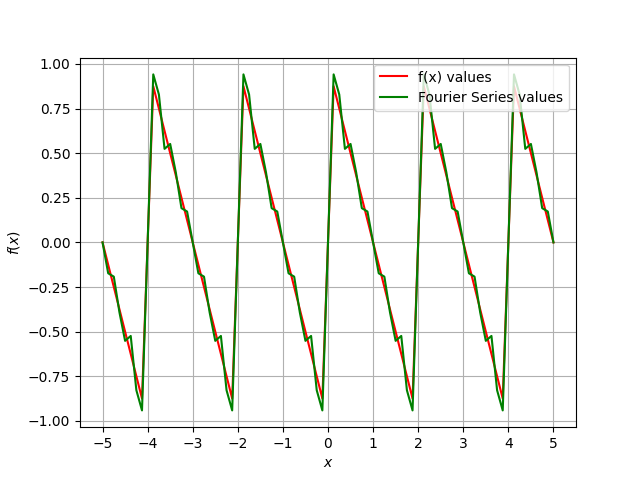
\includegraphics[width=\columnwidth]{./figs/f.png}
    \caption{}    
    \label{fig:ishitha.g22.in.13.f1}
\end{figure}
 

\end{document}

\item  A Simple closed path C in the Complex Plane is shown in the figure.
 \begin{align*}
        \oint_C \frac{2^z}{z^2-1}dz=-\jmath \pi A
 \end{align*}
 Where $\jmath=\sqrt{-1}$, Then find the value of A is \rule{1cm}{0.15mm}(Rounded of to two decimals)
\begin{figure}[h!]
    \centering
    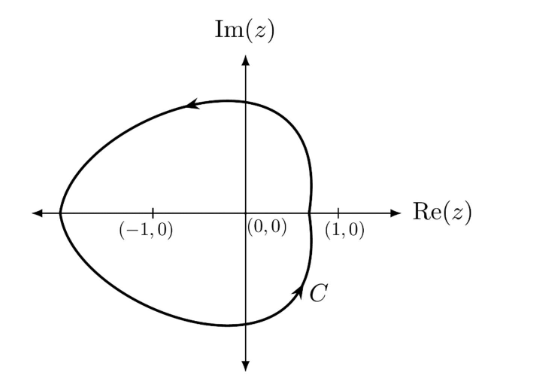
\includegraphics[width = \columnwidth]{2022/EC/32/figs/fig1.png}
\end{figure}
\hfill{(GATE 2022 EC)}\\
\solution 
\input{2022/EC/32/EC_32.tex}
\pagebreak
\item For the ideal AC-DC rectifier circuit shown in the figure below, the load current
magnitude is $I_{dc}$ = $15$ A and is ripple free. The thyristors are fired with a delay angle
of 45\degree
. The amplitude of the fundamental component of the source current, in
amperes, is \_\_\_\_\_\_\_\_{\em (Round off to 2
decimal places)}. \hfill(GATE 59 EE 2022)
\begin{figure}[!h]
\centering
 \begin{circuitikz}[scale = 0.8]
      \draw (-0.8,0.8) -- (-0.8,0.8) node[above]{$+$};
    \draw (0,2) to[sV] (0,-1);
     \draw (-0.8,0) -- (-0.8,0) node[below]{$-$};
    \draw (0,2) -- (2,2);
    \draw (2,2) -- (2,1);
    \draw (2,1) -- (3,1);
     \draw (3,1) to [thyristor] (3,3);
    \draw (3,3) -- (5,3);
    \draw (5,1) to [thyristor] (5,3);
    \draw (5,3) -- (7,3);
    \draw (7,3) to[resistor](7,1);
    \draw (7,1) -- (7,0);
    \draw(7,0) to [L](7,-2);
    \draw (7,-2) -- (3,-2);

    \draw (0, -1) -- (2,-1);
    \draw (2,-1) -- (2,0.4);
    \draw (2,0.4) -- (5,0.4);
    \draw (3,-2) to [Do] (3,0.4);
    \draw (3,0.4) -- (3,1);
    \draw (5,-2) to [Do] (5,0.4);
    \draw (5,0.4) -- (5,1);

     \draw[->] (6.5, 2) -- (6.5, 1) node[midway, left]{$I_{dc}$};
        \end{circuitikz}
\end{figure}
\solution

\iffalse
\let\negmedspace\undefined
\let\negthickspace\undefined
\documentclass[journal,12pt,onecolumn]{IEEEtran}
\usepackage{cite}
\usepackage{amsmath,amssymb,amsfonts,amsthm}
\usepackage{algorithmic}
\usepackage{graphicx}
\usepackage{textcomp}
\usepackage{xcolor}
\usepackage{txfonts}
\usepackage{listings}
\usepackage{enumitem}
\usepackage{mathtools}
\usepackage{gensymb}
\usepackage{comment}
\usepackage[breaklinks=true]{hyperref}
\usepackage{tkz-euclide} 
\usepackage{tikz}
\usepackage{circuitikz}
\usepackage{listings}
\usepackage{gvv} 
\usepackage{caption}
\def\inputGnumericTable{}                   

%\usepackage[latin1]{inputenc}                                
\usepackage{color}                                            
\usepackage{array}                                            
\usepackage{longtable}                                       
\usepackage{calc}                                             
\usepackage{multirow}                                         
\usepackage{hhline}                                           
\usepackage{ifthen}                                           
\usepackage{lscape}
\usepackage{tikz}
\usepackage{circuitikz}

\newtheorem{theorem}{Theorem}[section]
\newtheorem{problem}{Problem}
\newtheorem{proposition}{Proposition}[section]
\newtheorem{lemma}{Lemma}[section]
\newtheorem{corollary}[theorem]{Corollary}
\newtheorem{example}{Example}[section]
\newtheorem{definition}[problem]{Definition}
\newcommand{\BEQA}{\begin{eqnarray}}
\newcommand{\EEQA}{\end{eqnarray}}
\newcommand{\define}{\stackrel{\triangle}{=}}
\theoremstyle{remark}
\newtheorem{rem}{Remark}

\begin{document}

\bibliographystyle{IEEEtran}
\vspace{3cm}

\title{GATE: EE - 59.2022}
\author{EE23BTECH11013 - Avyaaz$^{*}$% <-this % stops a space 
}
\maketitle
% \newpage
% \bigskip

\renewcommand{\thefigure}{\arabic{figure}}
\renewcommand{\thetable}{\arabic{table}}

\large\textbf{\textsl{Question:}}
For the ideal AC-DC rectifier circuit shown in the figure below, the load current
magnitude is $I_{dc}$ = $15$ A and is ripple free. The thyristors are fired with a delay angle
of 45\degree
. The amplitude of the fundamental component of the source current, in
amperes, is \_\_\_\_\_\_\_\_{\em (Round off to 2
decimal places)}. \hfill(GATE 59 EE 2022)
\begin{figure}[!h]
\centering
\begin{circuitikz}[scale = 0.8]
      \draw (-0.8,0.8) -- (-0.8,0.8) node[above]{$+$};
    \draw (0,2) to[sV] (0,-1);
     \draw (-0.8,0) -- (-0.8,0) node[below]{$-$};
    \draw (0,2) -- (2,2);
    \draw (2,2) -- (2,1);
    \draw (2,1) -- (3,1);
     \draw (3,1) to [thyristor] (3,3);
    \draw (3,3) -- (5,3);
    \draw (5,1) to [thyristor] (5,3);
    \draw (5,3) -- (7,3);
    \draw (7,3) to[resistor](7,1);
    \draw (7,1) -- (7,0);
    \draw(7,0) to [L](7,-2);
    \draw (7,-2) -- (3,-2);

    \draw (0, -1) -- (2,-1);
    \draw (2,-1) -- (2,0.4);
    \draw (2,0.4) -- (5,0.4);
    \draw (3,-2) to [Do] (3,0.4);
    \draw (3,0.4) -- (3,1);
    \draw (5,-2) to [Do] (5,0.4);
    \draw (5,0.4) -- (5,1);

     \draw[->] (6.5, 2) -- (6.5, 1) node[midway, left]{$I_{dc}$};
        \end{circuitikz}

\end{figure}

\solution
\fi
\begin{table}[htbp]
\setlength{\extrarowheight}{4pt}
\setlength{\tabcolsep}{3pt}
\centering
\begin{tabular}{|c|c|c|}
\hline
\textbf{Parameter} & \textbf{Description}&\textbf{Value}\\
\hline 
$I_{dc}$& Load current & $15$A  \\
\hline
$\alpha$ &Firing angle&$45\degree$ \\
\hline
\end{tabular}

\caption{}
\label{tab:inputs.EE.59.2022}
\end{table}
% It is a Single phase symmetrical semi-converter.
% \begin{enumerate}[label={\roman*)}]
%     \item Load current magnitude $\brak{I_{dc}}$ = $15$A
%     \item Firing angle $\brak{\alpha} = 45\degree$
% \end{enumerate}
A symmetrical single phase semi converter is shown below,

\begin{figure}[!h]
\centering
    \begin{circuitikz}[scale = 0.8]
      \draw (-0.8,0.8) -- (-0.8,0.8) node[above]{$+$};
    \draw (0,2) to[sV,l=$V_s$] (0,-1);
     \draw (-0.8,0) -- (-0.8,0) node[below]{$-$};
    \draw (0,2) -- (2,2);
    \draw (2,2) -- (2,1);
    \draw (2,1) -- (3,1);
     \draw (3,1) to [thyristor] (3,3);
     \node at (2.4,2.3) {$T_1$};
    \draw (3,3) -- (5,3);
    \draw (5,1) to [thyristor] (5,3);
     \node at (4.4,2.3) {$T_2$};
    \draw (5,3) -- (7,3);
    \draw (7,3) to[resistor](7,1);
    \draw (7,1) -- (7,0);
    \draw(7,0) to [L](7,-2);
    \draw (7,-2) -- (3,-2);

    \draw (0, -1) -- (2,-1);
    \draw (2,-1) -- (2,0.4);
    \draw (2,0.4) -- (5,0.4);
    \draw (3,-2) to [Do] (3,0.4);
    \node at (3.8,-1) {$D_1$};
    \draw (3,0.4) -- (3,1);
    \draw (5,-2) to [Do] (5,0.4);
    \node at (5.8,-1) {$D_2$};
    \draw (5,0.4) -- (5,1);

     \draw[->] (6.5, 2) -- (6.5, 1) node[midway, left]{$I_{dc}$};
          \draw[->] (0.5, 2) -- (1, 2) ;
          \node at (1,1.6) {$I_s$};
          \node at (7.4,2) {$R$};
          \node at (7.4,-1.1) {$L$};

     \draw (8,2.8) -- (8,2.8) node[above]{$+$};
     \draw[->] (8,0.8) -- (8,2.8);
     \node at (8,0.5) {$V_o$};
     \draw[->] (8,0.2) -- (8,-1.8);
     \draw (8,-1.8) -- (8,-1.8) node[below]{$-$};
        \end{circuitikz}

\end{figure}

The Fourier series representation of supply current is given by:
\begin{align}
    i_s(t) = a_o +\sum_{n=1}^{\infty}C_n\sin({n\omega t} + \theta_n)\label{eq:gen_i_s}
\end{align}
 where,
 \begin{align}
 a_o &= \frac{1}{2\pi} \int_{0}^{2\pi} i_s(t)d\omega t \\
     C_n &= \sqrt{a_n^2 + b_n ^2}\label{eq:bino_coeff}\\
     \theta_n &= \tan^{-1}\left({\frac{a_n}{b_n}}\right)\label{eq: theta}
 \end{align}
\begin{align}
  \implies  a_o &= \frac{1}{2\pi}\int_{\alpha}^{\pi} I_o d\omega t - \int_{\pi + \alpha}^{2\pi} I_o d\omega t = 0\\
 \implies   a_n &= \frac{1}{\pi} \int_{\alpha}^{\pi}I_o\cos n\omega t d\omega t - \int_{\pi + \alpha}^{2\pi} I_o\cos{n\omega td\omega t}\\
 a_n &= 
 \begin{cases}
    \frac{-2I_o}{n\pi}\sin{n\alpha} & \text{for } n = 1,3,5...\\
     0 &\text{for } n = 2,4.....
    \end{cases}\\
 \implies   b_n &= \frac{1}{\pi}\int_{\alpha}^{\pi}I_o\sin n\omega t d\omega t - \int_{\pi + \alpha}^{2\pi} I_o\sin{n\omega td\omega t} \\
 b_n &= 
 \begin{cases}
     \frac{2I_o}{n\pi}\left(1 + \cos{n\alpha}\right) &\text{for } n = 1,3,5...\\
     0 &\text{for } n = 2, 4....
    \end{cases}
    \end{align}
From \eqref{eq:bino_coeff}:
\begin{align}
  \therefore  C_n &= \frac{2\sqrt{2}I_o}{n\pi}\left(\sqrt{1 + \cos{n\alpha}}\right)\\
  \implies  C_n &= \frac{4I_o}{n\pi}\cos{\frac{n\alpha}{2}}\label{eq:final_bino}
\end{align}
From \eqref{eq: theta}:
\begin{align}
    \theta_n &= \tan^{-1}\left(\frac{-\sin{n\alpha}}{1 + \cos{n\alpha}}\right)\\
    \implies \theta_n &= \frac{-n\alpha}{2}\label{eq:final_theta}
\end{align}

From \eqref{eq:gen_i_s},\eqref{eq:final_bino} and \eqref{eq:final_theta}:
\begin{align}
I_{s}(t) = \sum_{n=1,3,5...}^{\infty} \frac{4I_{o}}{n\pi}\cos{\frac{n\alpha}{2}}\sin{\left(n\omega t - \frac{n\alpha}{2}\right)}
\end{align}
% \begin{align}
% I_{s}(t) = \sum_{n=1,3,5...}^{\infty} \frac{4I_{dc}}{n\pi}\cos{\frac{n\alpha}{2}}\sin{\left(n\omega t - \frac{n\alpha}{2}\right)}
% \end{align}


% \begin{tikzpicture}[scale=1]
%     \draw[->] (0,0) -- (10,0) node[right] {$\omega t$};
%     \draw[->] (0,-2) -- (0,2) node[above] {$y$};
%     \draw[domain=0:10, smooth, variable=\x, black] plot ({\x},{sin(deg(\x))});
%     \foreach \x/\xtext in {1.57/\frac{\pi}{2},3.14/\pi,4.71/\frac{3\pi}{2},6.28/2\pi,7.85/\frac{7\pi}{2}} {
%         \draw (\x cm,0) -- (\x cm,0.1) node[below] {$\xtext$};
%     }
%     \foreach \y in {-1,1} {
%         \draw (1pt,\y cm-1.5) -- (-1pt,\y cm-1.5) node[left] {$\y$};
%     }
% \end{tikzpicture}

\begin{figure}[!h]
    \centering
    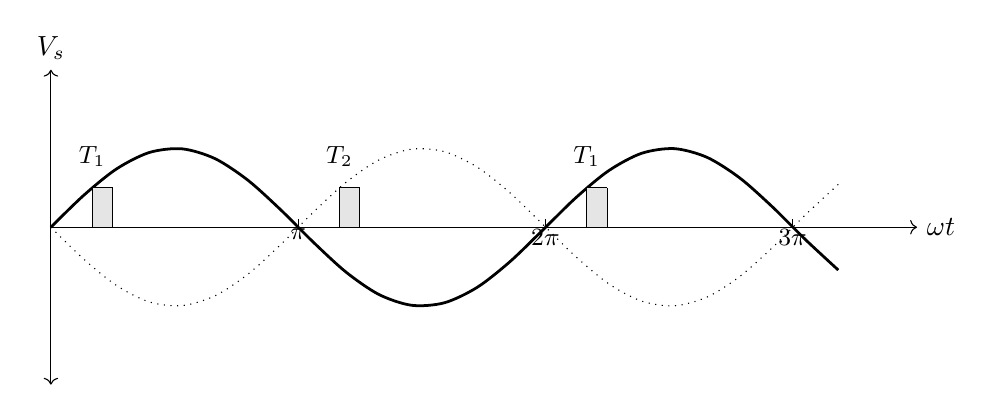
\begin{tikzpicture}[scale=1]
    \draw[->] (0,0) -- (11,0) node[right] {$\omega t$};
    \draw[<->] (0,-2) -- (0,2) node[above] {$V_s$};
    \draw[domain=0:10, smooth, variable=\x, black,line width=1pt] plot ({\x},{sin(deg(\x))});
    \draw[dotted,domain=0:10, smooth, variable=\x, black] plot ({\x},{-sin(deg(\x))});
    \foreach \x/\xtext in {3.14/\pi,6.28/2\pi,9.42/3\pi} {
        \draw (\x cm,0) -- (\x cm,0.1) node[below] {\small$\xtext$};
    }

\fill[gray!20] (0.5233,0) -- (0.5233,0.5) -- (0.785,0.5) -- (0.785,0) -- cycle;
    \fill[gray!20] (3.6633,0) -- (3.6633,0.5) -- (3.925,0.5) -- (3.925,0) -- cycle;
    \fill[gray!20] (6.8033,0) -- (6.8033,0.5) -- (7.065,0.5) -- (7.065,0) -- cycle;

    \draw (0.5233,0) -- (0.5233,0.5);
    \draw (0.5233,0.5) -- (0.785,0.5);
    \draw (0.785,0.5) -- (0.785,0);

    \draw (3.6633,0) -- (3.6633,0.5);
    \draw (3.6633,0.5) -- (3.925,0.5);
    \draw (3.925,0.5) -- (3.925,0);

    \draw (6.8033,0) -- (6.8033,0.5);
    \draw (6.8033,0.5) -- (7.065,0.5);
    \draw (7.065,0.5) -- (7.065,0);


     \node at (0.5233,0.9) {\small$T_1$};
     \node at (3.6633,0.9) {\small$T_2$};
     \node at (6.8033,0.9) {\small$T_1$};
\end{tikzpicture}
\end{figure}
\begin{figure}[!h]
    \centering
    \begin{tikzpicture}[scale=1]
    \draw[->] (0,0) -- (11,0) node[right] {$\omega t$};
    \draw[<->] (0,-2) -- (0,2) node[above] {$V_o$};
    \draw[domain=0.5233:3.14, smooth, variable=\x, black,line width=1pt] plot ({\x},{sin(deg(\x))});
    \draw[domain=3.6633:6.28, smooth, variable=\x, black,line width=1pt] plot ({\x},{-sin(deg(\x))});
    \draw[domain=6.8033:9.42, smooth, variable=\x, black,line width=1pt] plot ({\x},{sin(deg(\x))});

    \foreach \x/\xtext in {0.5233/\alpha, 3.14/\pi,4/\pi + \alpha ,6.28/2\pi,7.2/2\pi + \alpha,9.42/3\pi}{
        \draw (\x cm,0) -- (\x cm,0) node[below] {\small $\xtext$};
    }

     \draw [line width=1pt](0,0)--(0.5233,0);
    \draw [line width=1pt](0.5233,0) -- (0.5233,0.5);
    \draw[line width=1pt](3.14,0)-- (3.6633,0);
    \draw[line width=1pt] (3.6633,0) -- (3.6633,0.5);
    \draw [line width=1pt](6.28,0)--(6.8033,0);
    \draw [line width=1pt](6.8033,0) -- (6.8033,0.5);

    \node at (0.25,0.6){\small$T_2$};
    \node at (0.25,0.2){\small$D_2$};
     \node at (3.4,0.6){\small$T_1$};
    \node at (3.4,0.2){\small$D_1$};
    \node at (6.4,0.6){\small$T_2$};
    \node at (6.4,0.2){\small$D_2$};

    \node at (1.57,0.4){\small $T_1D_2$};
    \node at (4.71,0.4){\small $T_2D_1$};
    
\end{tikzpicture}
\end{figure}
\begin{figure}[!h]
    \centering
    \begin{tikzpicture}[scale=1]
    \draw[->] (0,0) -- (11,0) node[right] {$\omega t$};
    \draw[<->] (0,-2) -- (0,2) node[above] {$i_{T_1}$};
   
    \foreach \x/\xtext in {0.5233/\alpha,4/\pi + \alpha,7.2/2\pi + \alpha,10/3\pi + \alpha}{
        \draw (\x cm,0) -- (\x cm,0) node[below] {\small $\xtext$};
    }
     \draw [line width=1pt](0,0)--(0.5233,0);
    \draw [line width=1pt](0.5233,0) -- (0.5233,1);
    \draw[line width=1pt](0.5233,1)-- (3.6633,1);
    \draw[line width=1pt] (3.6633,1) -- (3.6633,0);
    \draw[line width=1pt] (3.6633,0) -- (6.8033,0);
    \draw [line width=1pt](6.8033,0)--(6.8033,1);
    \draw [line width=1pt](6.8033,1) -- (9.948,1);
     \draw [line width=1pt] (9.948,1) -- (9.948,0);

     \draw[dotted,domain=0:10, smooth, variable=\x, black] plot ({\x},{1});
     \node at (0.4,1.2) {\small $I_{DC}$};
\end{tikzpicture}
\end{figure}
\begin{figure}[!h]
    \centering
    \begin{tikzpicture}[scale=1]
    \draw[->] (0,0) -- (11,0) node[right] {$\omega t$};
    \draw[<->] (0,-2) -- (0,2) node[above] {$i_{s}$};
   

    \draw [line width=1pt](0.5233,0) -- (0.5233,1);
    \draw[line width=1pt](0.5233,1)-- (3.14,1);
    \draw[line width=1pt](3.14,1)-- (3.14,0);
    \draw[line width=1pt] (3.14,0) -- (3.6633,0);
    \draw[line width=1pt] (3.6633,0) -- (3.6633,-1);
    \draw[line width=1pt] (3.6633,-1) -- (6.28,-1);
    \draw[line width=1pt]  (6.28,-1) -- (6.28,0);
    \draw[line width=1pt] (6.28,0) -- (6.8033,0);
    \draw [line width=1pt](6.8033,0)--(6.8033,1);
    \draw [line width=1pt](6.8033,1) -- (9.42,1);
     \draw [line width=1pt] (9.42,1) -- (9.42,0);
     \draw [line width=1pt] (9.42,0) -- (9.948,0);

     \draw[dotted,domain=0:10, smooth, variable=\x, black] plot ({\x},{1});
     \node at (0.4,1.2) {\small $I_{DC}$};
    
\end{tikzpicture}
\end{figure}

From \tabref{tab:inputs.EE.59.2022}:
\begin{align}
   (I_{s_1})_{peak} &= \frac{4I_{dc}}{\pi}\cos{\left(\frac{\alpha}{2}\right)}\\
    &= \frac{4 \times 15 }{\pi}\times \cos{\frac{45 \degree}{2}}\\
    &=17.64 A 
\end{align}

%\end{document}

\pagebreak

\item The fourier series expansion of $x^3$ in the interval $-1\leq x\leq 1$with periodic continuation has
\begin{enumerate}[label=(\alph*)]
    \item only sine terms
    \item only cosine terms
    \item both sine and cosine terms
    \item only sine terms and a non-zero constant
\end{enumerate} \hfill(GATE 2022 ME)    \\
\solution
% \iffalse
\let\negmedspace\undefined
\let\negthickspace\undefined
\documentclass[journal,12pt,twocolumn]{IEEEtran}
\usepackage{cite}
\usepackage{amsmath,amssymb,amsfonts,amsthm}
\usepackage{algorithmic}
\usepackage{graphicx}
\usepackage{textcomp}
\usepackage{xcolor}
\usepackage{pgfplots}
\usepackage{txfonts}
\usepackage{listings}
\usepackage{enumitem}
\usepackage{mathtools}
\usepackage{gensymb}
\usepackage{comment}
\usepackage[breaklinks=true]{hyperref}
\usepackage{tkz-euclide} 
\usepackage{listings}
\usepackage{gvv}                                        
\def\inputGnumericTable{}                                 
\usepackage[latin1]{inputenc}                                
\usepackage{color}                                            
\usepackage{array}                                            
\usepackage{longtable}                                       
\usepackage{calc}                                             
\usepackage{multirow}                                         
\usepackage{hhline}                                           
\usepackage{ifthen}                                           
\usepackage{lscape}

\newtheorem{theorem}{Theorem}[section]
\newtheorem{problem}{Problem}
\newtheorem{proposition}{Proposition}[section]
\newtheorem{lemma}{Lemma}[section]
\newtheorem{corollary}[theorem]{Corollary}
\newtheorem{example}{Example}[section]
\newtheorem{definition}[problem]{Definition}
\newcommand{\BEQA}{\begin{eqnarray}}
\newcommand{\EEQA}{\end{eqnarray}}
\newcommand{\define}{\stackrel{\triangle}{=}}
\theoremstyle{remark}
\newtheorem{rem}{Remark}
\begin{document}
\parindent 0px
\bibliographystyle{IEEEtran}
\title{GATE: ME - 14.2022}
\author{EE22BTECH11219 - Rada Sai Sujan$^{}$% <-this % stops a space
}
\maketitle
\newpage
\bigskip
\section*{Question}
The fourier series expansion of $x^3$ in the interval $-1\leq x\leq 1$with periodic continuation has
\begin{enumerate}[label=(\alph*)]
    \item only sine terms
    \item only cosine terms
    \item both sine and cosine terms
    \item only sine terms and a non-zero constant
\end{enumerate} \hfill(GATE 2022 ME)    \\
\solution

Fourier series expansion of the function $x\brak{t}$ in the interval $[-L,L]$ can be given by: \\
\begin{align}
    x\brak{t}=a_0+\sum\limits_{n=1}^{\infty}a_n\cos\brak{\frac{n\pi t}{L}}+\sum\limits_{n=1}^{\infty}b_n\sin\brak{\frac{n\pi t}{L}}
\end{align}
where,
\begin{align}
    a_0&=\frac{1}{2L}\int\limits_{-L}^{L}f\brak{t}\,dt  \\
    a_n&=\frac{1}{2L}\int\limits_{-L}^{L}f\brak{t}\cos\brak{\frac{n\pi t}{L}}\,dt  \\
    b_n&=\frac{1}{2L}\int\limits_{-L}^{L}f\brak{t}\sin\brak{\frac{n\pi t}{L}}\,dt  \\
\end{align}
Therefore, the expansion can be given by:
\begin{align}
    t^3=a_0+\sum\limits_{n=1}^{\infty}a_n\cos\brak{n\pi t}+\sum\limits_{n=1}^{\infty}b_n\sin\brak{n\pi t}
\end{align}
Since $t^3$ is an odd function,
\begin{align}
    a_0&=a_n=0   \\
    b_n&=\frac{1}{2}\int\limits_{-1}^{1}t^3\sin\brak{n\pi t}\,dt    \\
    &=\brak{-1}^{n+1}\brak{\frac{2}{n\pi}-\frac{12}{\brak{n\pi}^3}} \
\end{align}
\begin{align}
    \implies t^3&=\sum\limits_{n=1}^{\infty}b_n\sin\brak{\frac{n\pi t}{L}}
\end{align}
$\therefore$It contains only sine terms.
\end{document}

\pagebreak

\item The discrete time Fourier series representation of a signal $x[n]$ with period $N$ is written as  $x[n]=\sum_{k=0}^{N-1}a_ke^{j\brak{2kn\pi/N}}$ . A discrete time periodic signal with period $N=3$, has the non-zero Fourier series coefficients: $a_{-3}=2$ and $a_4=1$. The signal is
\begin{enumerate}[label=(\Alph*)]
\item $2+2e^{-\brak{j\frac{2\pi}{6}n}}\cos{\brak{\frac{2\pi}{6}n}}$
\item $1+2e^{\brak{j\frac{2\pi}{6}n}}\cos{\brak{\frac{2\pi}{6}n}}$
\item $1+2e^{\brak{j\frac{2\pi}{3}n}}\cos{\brak{\frac{2\pi}{6}n}}$
\item $2+2e^{\brak{j\frac{2\pi}{6}n}}\cos{\brak{\frac{2\pi}{6}n}}$
\end{enumerate}
\hfill(GATE EE 2022)
\\
\solution
\iffalse
\let\negmedspace\undefined
\let\negthickspace\undefined
\documentclass[journal,12pt,twocolumn]{IEEEtran}
\usepackage{cite}
\usepackage{amsmath,amssymb,amsfonts,amsthm}
\usepackage{algorithmic}
\usepackage{graphicx}
\usepackage{textcomp}
\usepackage{xcolor}
\usepackage{txfonts}
\usepackage{listings}
\usepackage{enumitem}
\usepackage{mathtools}
\usepackage{gensymb}
\usepackage{comment}
\usepackage[breaklinks=true]{hyperref}
\usepackage{tkz-euclide} 
\usepackage{listings}
\usepackage{gvv}                                        
\def\inputGnumericTable{}                                 
\usepackage[latin1]{inputenc}                                
\usepackage{color}                                            
\usepackage{array}                                            
\usepackage{longtable}                                       
\usepackage{calc}                                             
\usepackage{multirow}                                         
\usepackage{hhline}                                           
\usepackage{ifthen}                                           
\usepackage{lscape}
\newtheorem{theorem}{Theorem}[section]
\newtheorem{problem}{Problem}
\newtheorem{proposition}{Proposition}[section]
\newtheorem{lemma}{Lemma}[section]
\newtheorem{corollary}[theorem]{Corollary}
\newtheorem{example}{Example}[section]
\newtheorem{definition}[problem]{Definition}
\newcommand{\BEQA}{\begin{eqnarray}}
\newcommand{\EEQA}{\end{eqnarray}}
\newcommand{\define}{\stackrel{\triangle}{=}}
\theoremstyle{remark}
\newtheorem{rem}{Remark}
\begin{document}

\bibliographystyle{IEEEtran}
\vspace{3cm}

\title{GATE: EE - 49.2022}
\author{EE23BTECH11224 - Sri Krishna Prabhas Yadla$^{*}$% <-this % stops a space
}
\maketitle
\newpage
\bigskip

\renewcommand{\thefigure}{\arabic{figure}}
\renewcommand{\thetable}{\arabic{table}}


\vspace{3cm}
\textbf{Question:} The discrete time Fourier series representation of a signal $x[n]$ with period $N$ is written as  $x[n]=\sum_{k=0}^{N-1}a_ke^{j\brak{2kn\pi/N}}$ . A discrete time periodic signal with period $N=3$, has the non-zero Fourier series coefficients: $a_{-3}=2$ and $a_4=1$. The signal is
\begin{enumerate}[label=(\Alph*)]
\item $2+2e^{-\brak{j\frac{2\pi}{6}n}}\cos{\brak{\frac{2\pi}{6}n}}$
\item $1+2e^{\brak{j\frac{2\pi}{6}n}}\cos{\brak{\frac{2\pi}{6}n}}$
\item $1+2e^{\brak{j\frac{2\pi}{3}n}}\cos{\brak{\frac{2\pi}{6}n}}$
\item $2+2e^{\brak{j\frac{2\pi}{6}n}}\cos{\brak{\frac{2\pi}{6}n}}$
\end{enumerate}
\hfill(GATE EE 2022)
\\
\solution
\fi
\begin{table}[htbp]
	\centering
	\def\arraystretch{1.5}
	\begin{tabular}{|c|c|c|}
\hline
\textbf{Parameters} & \textbf{Description} & \textbf{Value} \\
\hline
$x[n]$ & Signal & \\
\hline
$N$ & Period & 3 \\
\hline
$a_k$ & Fourier series coefficient &\\
\hline
$a_{-3}$ & $a_k$ at $k=-3$ & 2 \\
\hline
$a_4$ & $a_k$ at $k=4$ & 1 \\
\hline
\end{tabular}

	\caption{Parameters}
	\label{tab:parameters_ee_49}
\end{table}

\begin{align}
x[n] &= \sum_{k=-\infty}^{\infty}a_ke^{j\brak{\frac{2k\pi}{3}n}} \\
&= a_{-3}e^{j\frac{-6\pi}{3}n} + a_{4}e^{j\frac{8\pi}{3}n}  \\
&= 2 + e^{j\frac{2\pi}{3}n}\\
&= 1+1+e^{j\frac{2\pi}{3}n}\\
&= 1+e^{j\frac{2\pi}{6}n}e^{-j\frac{2\pi}{6}n}+e^{j\frac{2\pi}{6}n}e^{j\frac{2\pi}{6}n}\\
&= 1+2e^{j\frac{2\pi}{6}n}\brak{\frac{e^{j\frac{2\pi}{6}n}+e^{-j\frac{2\pi}{6}n}}{2}} \\
&= 1+2e^{j\frac{2\pi}{6}n}\cos{\brak{\frac{2\pi}{6}n}}
\end{align}
\begin{figure}[htbp]
	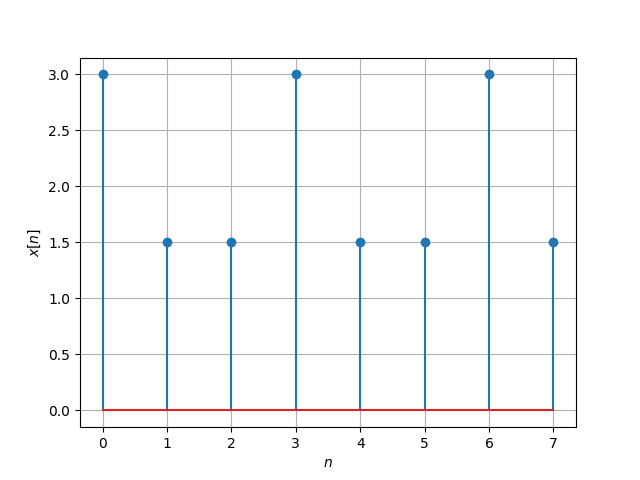
\includegraphics[width=\columnwidth]{2022/EE/49/figs/plot.png}
	\caption{Stem Plot of $x[n]$}
	\label{fig:plot_ee49}
\end{figure}

\pagebreak
\end{enumerate}

 \section{2021}
 \begin{enumerate}[label=\thechapter.\arabic*,ref=\thechapter.\theenumi]
\item Consider the signals $x\brak{n}$=$2^{n-1} u\brak{ -n+2}$ and $y\brak{n}$=$2^{-n+2}u\brak{ n+1}$, where $u\brak{n}$ is the unit step sequence. Let $X\brak{e^{j\omega}}$ and $Y\brak{e^{j\omega}}$ be the discrete-time Fourier of $x\brak{n}$ and $y\brak{n}$,respectively. The value of the integral $\frac{1}{2\pi}\int_{0}^{2\pi} X\brak{e^{j\omega}} Y\brak{e^{-j\omega}} d \omega$
(rounded off to one decimal place) is \underline{{\hspace{1.5in}}}\\
\hfill{(GATE EC 41 2021)}\\
\solution

\let\negmedspace\undefined
\let\negthickspace\undefined
\documentclass[journal,12pt,twocolumn]{IEEEtran}
\usepackage{cite}
\usepackage{amsmath,amssymb,amsfonts,amsthm}
\usepackage{algorithmic}
\usepackage{graphicx}
\usepackage{textcomp}
\usepackage{xcolor}
\usepackage{txfonts}
\usepackage{listings}
\usepackage{enumitem}
\usepackage{mathtools}
\usepackage{gensymb}
\usepackage{comment}
\usepackage[breaklinks=true]{hyperref}
\usepackage{tkz-euclide} 
\usepackage{listings}
\usepackage{gvv}                                        
\def\inputGnumericTable{}                                 
\usepackage[latin1]{inputenc}                                
\usepackage{color}                                            
\usepackage{array}                                            
\usepackage{longtable}                                       
\usepackage{calc}                                             
\usepackage{multirow}                                         
\usepackage{hhline}                                           
\usepackage{ifthen}                                           
\usepackage{lscape}

\newtheorem{theorem}{Theorem}[section]
\newtheorem{problem}{Problem}
\newtheorem{proposition}{Proposition}[section]
\newtheorem{lemma}{Lemma}[section]
\newtheorem{corollary}[theorem]{Corollary}
\newtheorem{example}{Example}[section]
\newtheorem{definition}[problem]{Definition}
\newcommand{\BEQA}{\begin{eqnarray}}
\newcommand{\EEQA}{\end{eqnarray}}
\newcommand{\define}{\stackrel{\triangle}{=}}
\theoremstyle{remark}
\newtheorem{rem}{Remark}
\begin{document}
\bibliographystyle{IEEEtran}
\vspace{3cm}
\title{\textbf{EC-2021}}
\author{EE23BTECH11210-Dhyana Teja Machineni$^{*}$% <-this % stops a space
}
\maketitle
\newpage
\bigskip

\textbf{QUESTION:}\\
Consider the signals $x\brak{n}$=$2^{n-1} u\brak{ -n+2}$ and $y\brak{n}$=$2^{-n+2}u\brak{ n+1}$, where $u\brak{n}$ is the unit step sequence. Let $X\brak{e^{j\omega}}$ and $Y\brak{e^{j\omega}}$ be the discrete-time Fourier of $x\brak{n}$ and $y\brak{n}$,respectively. The value of the integral $\frac{1}{2\pi}\int_{0}^{2\pi} X\brak{e^{j\omega}} Y\brak{e^{-j\omega}} d \omega$
(rounded off to one decimal place) is \underline{{\hspace{1.5in}}}\\
\hfill{(GATE EC 41 2021)}\\

\solution\\

\begin{table}[h]
         
\begin{tabular}{|c|c|l|}
\hline
Parameter  & Value & Description   \\             
\hline
$y(0)$     & $0$   & Initial displacement  \\     
 \hline
$y'(0)$    & $0$   & First derivative at $t=0$  \\
 \hline
$y''(0)$   & $0$   & Second derivative at $t=0$ \\
 \hline
$y'''(0)$  & $0$   & Third derivative at $t=0$  \\
 \hline
\end{tabular}


         \caption{Variables and their descriptions}
     \end{table}
\begin{align}
    V&=\frac{1}{2\pi}\int_{0}^{2\pi} X\brak{e^{j\omega}} Y\brak{e^{-j\omega}} d \omega\\
     Z\brak{e^{j\omega}}&= X\brak{e^{j\omega}} Y\brak{e^{-j \omega}}\\
           z(n)&\xrightarrow{\mathcal{F}} Z(e^{j\omega})\\
           z\brak{n}&=\frac{1}{2\pi}\int_{-\pi}^{\pi} Z\brak{e^{j\omega}} e^{j\omega n} d\omega\\
      z\brak{0}&=\frac{1}{2\pi}\int_{0}^{2\pi} Z\brak{e^{j\omega}} d \omega\\
   z\brak{ n}&= x\brak{n} * y\brak{-n}\\
   &=\sum_{k=-\infty}^{\infty} 2^{k-1} u\brak{-k+2} 2^{n-k+2} u\brak{-n+k+1}\\
   &=\sum_{k=-\infty}^{2} 2^{n+1} u\brak{k-n+1}\\
   z(0)&=\sum_{k=-\infty}^{2} 2 u\brak{k+1}\\
   &=2\sum_{k=-1}^{2}u\brak{k+1}\\
  \therefore z\brak{0} &=8
\end{align}
$\therefore$ $\frac{1}{2\pi}\int_{0}^{2\pi} X\brak{e^{j\omega}} Y\brak{e^{-j\omega}} d \omega$= $8$
\renewcommand{\thefigure}{\theenumi}
 \renewcommand{\thetable}{\theenumi}
\begin{figure}[h]
  
  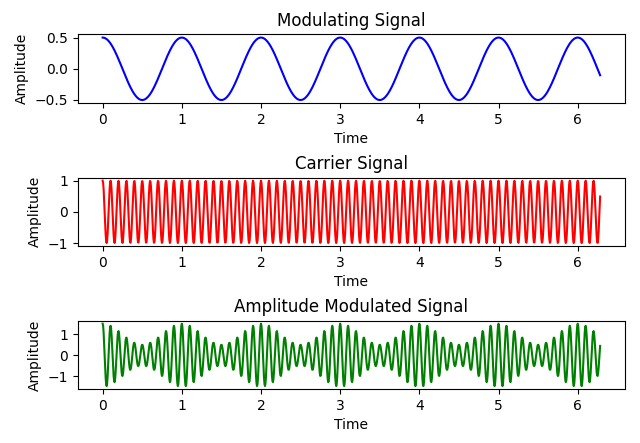
\includegraphics[width=\columnwidth]{figs/Figure_1.png}
  \caption{Stem Plot of $z\brak{n}$}
\end{figure}
\end{document}

\pagebreak
\item Given that $\mathcal{S}$ is the unit circle in the counter clock-wise direction with its centre at origin, the integral
        $\oint \brak{\frac{z^3}{4z-\jmath}}dz=\rule{1cm}{0.15mm}$
 (round off to theree decimal places)
 \hfill{(GATE 2022 AE)}\\
 \solution\\
 


\item Consider the signals \(x[n] = 2^{n-1} u[-n+2]\) and \(y[n] = 2^{-n+2} u[n+1]\), where \(u[n]\) is the unit step sequence. Let \(X(e^{j\omega})\) and \(Y(e^{j\omega})\) be the discrete-time Fourier transform of \(x[n]\) and \(y[n]\), respectively. The value of the integral
\[
\frac{1}{2\pi} \int_{0}^{2\pi} X(e^{j\omega}) Y(e^{-j\omega}) d\omega
\]
(rounded off to one decimal place) is.\\
\hfill{GATE 2021 EC 41 Q}
\solution
\iffalse
\let\negmedspace\undefined
\let\negthickspace\undefined
\documentclass[journal,12pt,twocolumn]{IEEEtran}
\usepackage{pgfplots}
\pgfplotsset{compat=1.17}
\usepackage{cite}
\usepackage{amsmath,amssymb,amsfonts,amsthm}
\usepackage{algorithmic}
\usepackage{graphicx}
\usepackage{textcomp}
\usepackage{xcolor}
\usepackage{txfonts}
\usepackage{listings}
\usepackage{enumitem}
\usepackage{mathtools}
\usepackage{gensymb}
\usepackage{comment}
\usepackage[breaklinks=true]{hyperref}
\usepackage{tkz-euclide} 
\usepackage{listings}
\usepackage{gvv}                                        
\def\inputGnumericTable{}                                 
\usepackage[latin1]{inputenc}                                
\usepackage{color}                                            
\usepackage{array}                                            
\usepackage{longtable}                                       
\usepackage{calc}                                             
\usepackage{multirow}                                         
\usepackage{hhline}                                           
\usepackage{ifthen}                                           
\usepackage{lscape}
\newtheorem{theorem}{Theorem}[section]
\newtheorem{problem}{Problem}
\newtheorem{proposition}{Proposition}[section]
\newtheorem{lemma}{Lemma}[section]
\newtheorem{corollary}[theorem]{Corollary}
\newtheorem{example}{Example}[section]
\newtheorem{definition}[problem]{Definition}
\newcommand{\BEQA}{\begin{eqnarray}}
\newcommand{\EEQA}{\end{eqnarray}}
\newcommand{\define}{\stackrel{\triangle}{=}}
\theoremstyle{remark}
\newtheorem{rem}{Remark}
\begin{document}
\bibliographystyle{IEEEtran}
\vspace{3cm}
\title{GATE EC 41Q}
\author{EE23BTECH11021 - GANNE GOPI CHANDU$^{*}$% <-this % stops a space
}
\maketitle
\bigskip
\renewcommand{\thefigure}{\theenumi}
\renewcommand{\thetable}{\theenumi}
\bibliographystyle{IEEEtran}
\textbf{Question}\\
Consider the signals \(x[n] = 2^{n-1} u[-n+2]\) and \(y[n] = 2^{-n+2} u[n+1]\), where \(u[n]\) is the unit step sequence. Let \(X(e^{j\omega})\) and \(Y(e^{j\omega})\) be the discrete-time Fourier transform of \(x[n]\) and \(y[n]\), respectively. The value of the integral
\[
\frac{1}{2\pi} \int_{0}^{2\pi} X(e^{j\omega}) Y(e^{-j\omega}) d\omega
\]
(rounded off to one decimal place) is.\\
\textbf{Solution}\\
\fi
\begin{table}[!h]
\begin{center}
\renewcommand\thetable{1}
\begin{tabular}{ |c|c|c| } 
  \hline
    Symbol & Value & description \\ 
  \hline
  $x[n] $ & $2^{n-1}u[-n+2]$ & Discrete time signal  \\ 
  \hline
  $y[n] $ & $2^{-n+2}u[n+1]$ & Discrete time signal  \\ 
  \hline
\end{tabular}
\end{center}
\caption{}
\end{table}
\begin{align}
     x[n]*y[n] && \xleftrightarrow[transform]{Fourier} && X(e^{j\omega}) Y(e^{j\omega})\\
 x[n] && \xleftrightarrow [transform]{Fourier} && X(e^{j\omega}) \\
 y[n] && \xleftrightarrow [transform]{Fourier} && Y(e^{j\omega}) 
\end{align}
The
 \begin{align}
       y(n) && \xleftrightarrow [transform]{Fourier} && y(e^{j\omega})
\end{align}
By using the time reversal property:
\begin{align}
y[-n] && \xleftrightarrow [transform]{Fourier} && y(e^{-j\omega})
\end{align}
Let assume
\begin{align}
     z[n]& = x[n] * y[-n]\\
     Z\brak{e^{j \omega}} &=X(e^{j\omega}) Y(e^{-j\omega})
 \end{align}
\begin{align}
      z[n]& =\frac{1}{2\pi} \int_{0}^{2\pi} Z(e^{j\omega})e^{j \omega n} d\omega \\
      &=\frac{1}{2\pi} \int_{0}^{2\pi}  X(e^{j\omega}) Y(e^{-j\omega})e^{j \omega n} d\omega.
 \end{align}
 putting  n=0, we get
\begin{align}
    z[0]&=\frac{1}{2\pi} \int_{0}^{2\pi} X(e^{j\omega}) Y(e^{-j\omega}) d\omega
\end{align}
\begin{align}
    z[n] = x[n] * y[-n]\\
 &= \sum_{k=-\infty}^{\infty} 2^{k-1} u[-k+2]\cdot 2^{n-k+2} u[-n+k+1]\\
 &= \sum_{k=-\infty}^{2} 2^{k-1} \cdot 2^{n-k+2} u[-n+k+1]\\
 &= \sum_{k=-\infty}^{2} 2^{k-1+n-k+2} u[-n+k+1]\\
 &= \sum_{k=-\infty}^{2} 2^{n+1} u[-n+k+1]
\end{align}

Putting $n = 0$, we get:
\begin{align}
     \frac{1}{2\pi} \int_{0}^{2\pi} X(e^{j\omega}) Y(e^{-j\omega}) d\omega &= z[0]\\
     &= \sum_{k=-\infty}^{2} 2 \cdot u[k+1] \\
     &=\sum_{k=-1}^{2} 2(1) = 2 \times 4 \\
     &= 8
\end{align}

\pagebreak
\item Consider a continuous-time signal $x\brak{t}$ \,defined by $x\brak{t}=0$\,for $\abs{t}>1$, and $x\brak{t}=1-\abs{t}$ for $\abs{t}\le 1$. Let the Fourier transform of $x\brak{t}$ be defined as $X\brak{\omega}=\int_{-\infty}^{\infty}x\brak{t}e^{-j\omega t} dt$. The maximum magnitude of $X\brak{\omega}$ is $\hbox to 4em{\thinspace\hrulefill\thinspace}$.
\hfill{(GATE 2021 EE 43)}\\
\solution
%\iffalse
\let\negmedspace\undefined
\let\negthickspace\undefined
\documentclass[journal,12pt,onecolumn]{IEEEtran}
\usepackage{cite}
\usepackage{amsmath,amssymb,amsfonts,amsthm}
\usepackage{algorithmic}
\usepackage{graphicx}
\usepackage{textcomp}
\usepackage{xcolor}
\usepackage{txfonts}
\usepackage{listings}
\usepackage{enumitem}
\usepackage{mathtools}
\usepackage{gensymb}
\usepackage{comment}
\usepackage{caption}
\usepackage[breaklinks=true]{hyperref}
\usepackage{tkz-euclide} 
\usepackage{listings}
\usepackage{gvv}                                        
\def\inputGnumericTable{}                                 
\usepackage[latin1]{inputenc}                                
\usepackage{color}                                            
\usepackage{array}                                            
\usepackage{longtable}                                       
\usepackage{calc}                                             
\usepackage{multirow}                                         
\usepackage{hhline}                                           
\usepackage{ifthen}                                           
\usepackage{lscape}

\newtheorem{theorem}{Theorem}[section]
\newtheorem{problem}{Problem}
\newtheorem{proposition}{Proposition}[section]
\newtheorem{lemma}{Lemma}[section]
\newtheorem{corollary}[theorem]{Corollary}
\newtheorem{example}{Example}[section]
\newtheorem{definition}[problem]{Definition}
\newcommand{\BEQA}{\begin{eqnarray}}
\newcommand{\EEQA}{\end{eqnarray}}
\newcommand{\define}{\stackrel{\triangle}{=}}
\theoremstyle{remark}
\newtheorem{rem}{Remark}
\begin{document}

\bibliographystyle{IEEEtran}
\vspace{3cm}

\title{GATE 2021 EE 43}
\author{EE23BTECH11022 - G DILIP REDDY}
\maketitle

\bigskip

\renewcommand{\thefigure}{\arabic{figure}}
\renewcommand{\thetable}{\arabic{table}}
\textbf{Question}:\\
Consider a continuous-time signal $x\brak{t}$ \,defined by $x\brak{t}=0$\,for $\abs{t}>1$, and $x\brak{t}=1-\abs{t}$ for $\abs{t}\le 1$. Let the Fourier transform of $x\brak{t}$ be defined as $X\brak{\omega}=\int_{-\infty}^{\infty}x\brak{t}e^{-j\omega t} dt$. The maximum magnitude of $X\brak{\omega}$ is $\hbox to 4em{\thinspace\hrulefill\thinspace}$.
\hfill{(GATE 2021 EE 43)}
\\\\
\solution
%\fi
\begin{align}
X\brak{f}&=\int_{-\infty}^{\infty}x\brak{t}e^{-j2\pi f t} dt\\
X\brak{f}&=\int_{-1}^{1}\brak{1-\abs{t}}e^{-j2\pi f t} dt\\
X\brak{f}&=\int_{-1}^{1}e^{-j2\pi f t} 
dt - \int_{-1}^{1}\abs{t}e^{-j2\pi f t} dt\\
X\brak{f}&=2\int_{0}^{1}\cos\brak{{2\pi f t}}
dt - 2\int_{0}^{1}t\cos\brak{2\pi f t} dt\\
X\brak{f}&=2\frac{\sin\brak{{2\pi f }}}{2\pi f}
- 2\sbrak{\frac{\sin\brak{2\pi f }}{2\pi f}+\frac{\cos\brak{2\pi f }}{\brak{2\pi f}^2}-\frac{1}{\brak{2\pi f }^2}}\\
X\brak{f}&=2\frac{1-\cos\brak{2\pi f }}{\brak{2\pi f}^2}\\
X\brak{f}&=2\frac{2\sin^2\brak{\frac{2\pi f}{2}}}{\brak{2\pi f}^2}\\
X\brak{f}&=\frac{\sin^2\brak{\pi f}}{\brak{\pi f}^2}\\
f& \to 0 \implies X\brak{f}\to1
\end{align}
Maximum of magnitude of $X\brak{f}=1$
\begin{figure}[h]
    \centering
    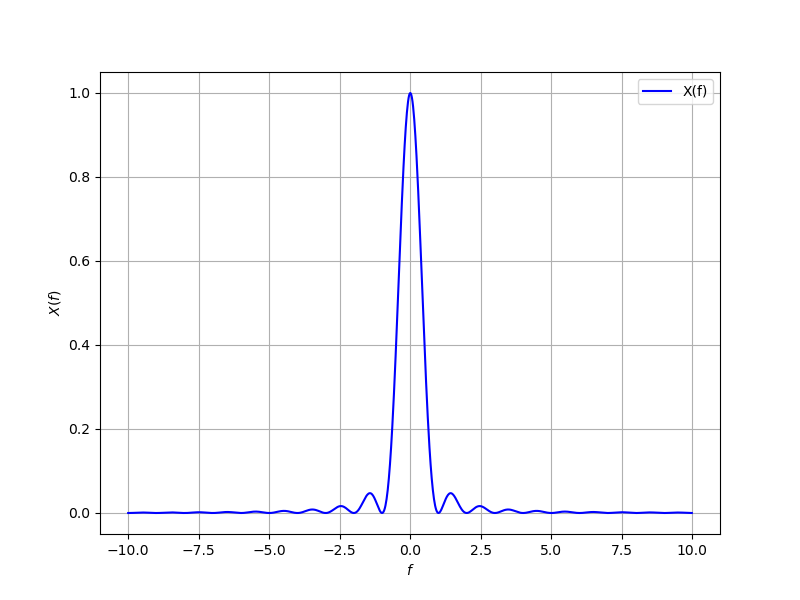
\includegraphics[width=1\linewidth]{figs/graph.png}
    \caption{plot of X(f)}
\end{figure}
\end{document}
\pagebreak
\item Let $f(t)$ be an even function, i.e.$f(-t) = f(t)$ for all t.Let the Fourier transform of $f(t)$ be defined as $F(\omega) = \int_{-\infty}^{\infty} f(t) e^{-j \omega t} \, dt $ . Suppose $\dfrac{dF(\omega)}{d \omega} = -\omega F(\omega)$ for all $\omega$ , and $F(0) = 1$ . Then


\begin{enumerate}[label = (\Alph*)]
\item $f(0) < 1 $\\
\item  $f(0) > 1 $\\
\item  $f(0) = 1 $\\
\item   $f(0) = 0 $\\
\end{enumerate} \hfill{(GATE EE 2021)}\\
\solution
\let\negmedspace\undefined
\let\negthickspace\undefined
\documentclass[journal,12pt,twocolumn]{IEEEtran}
\usepackage{cite}
\usepackage{amsmath,amssymb,amsfonts,amsthm}
\usepackage{algorithmic}
\usepackage{graphicx}
\usepackage{textcomp}
\usepackage{xcolor}
\usepackage{txfonts}
\usepackage{listings}
\usepackage{enumitem}
\usepackage{mathtools}
\usepackage{gensymb}
\usepackage{comment}
\usepackage[breaklinks=true]{hyperref}
\usepackage{tkz-euclide} 
\usepackage{listings}
\usepackage{gvv}  
\usepackage{tikz}
\usepackage{circuitikz} 
\usepackage{caption}
\def\inputGnumericTable{}              
\usepackage[latin1]{inputenc}          
\usepackage{color}                    
\usepackage{array}                     
\usepackage{longtable}                 
\usepackage{calc}                     \usepackage{multirow}                  
\usepackage{hhline}                    
\usepackage{ifthen}                    
\usepackage{lscape}
\usepackage{amsmath}
\newtheorem{theorem}{Theorem}[section]
\newtheorem{problem}{Problem}
\newtheorem{proposition}{Proposition}[section]
\newtheorem{lemma}{Lemma}[section]
\newtheorem{corollary}[theorem]{Corollary}
\newtheorem{example}{Example}[section]
\newtheorem{definition}[problem]{Definition}
\newcommand{\BEQA}{\begin{eqnarray}}
\newcommand{\EEQA}{\end{eqnarray}}
\newcommand{\define}{\stackrel{\triangle}{=}}
\theoremstyle{remark}
\newtheorem{rem}{Remark}

%\bibliographystyle{ieeetr}
\begin{document}
%

\bibliographystyle{IEEEtran}




\title{
%	\logo{
G.A.T.E.

\large{EE1205 : Signals and Systems}

Indian Institute of Technology Hyderabad
%	}
}
\author{Chirag Garg

(EE23BTECH11206)
}	





\maketitle

\newpage



\bigskip

\renewcommand{\thefigure}{\theenumi}
\renewcommand{\thetable}{\theenumi}


\section{Question E.E.(32)}
\vspace{0.5cm}



\textbf{Question:} 
Let $f(t)$ be an even function, i.e.$f(-t) = f(t)$ for all t.Let the Fourier transform of $f(t)$ be defined as $F(\omega) = \int_{-\infty}^{\infty} f(t) e^{-j \omega t} \, dt $ . Suppose $\dfrac{dF(\omega)}{d \omega} = -\omega F(\omega)$ for all $\omega$ , and $F(0) = 1$ . Then


\begin{enumerate}[label = (\Alph*)]
\item $f(0) < 1 $\\
\item  $f(0) > 1 $\\
\item  $f(0) = 1 $\\
\item   $f(0) = 0 $\\
\end{enumerate} \hfill{(GATE EE 2021)}\\
%\section{Solution} 
\textbf{Solution: }
Given, \begin{align}
\dfrac{dF(\omega)}{d \omega} &= -\omega F(\omega) \\
\dfrac{dF(\omega)}{d \omega} + \omega F(\omega) &= 0 \\
ln|F(\omega)| &= -\dfrac{\omega^{2}}{2} + c \\
F(\omega) &= Ke^{-\frac{\omega^2}{2}}
\end{align}
Put $\omega = 0$ , \begin{align}
F(0) &= K \\
K&=1
\end{align}
\begin{align}
\therefore F(\omega) &= e^{-\frac{\omega^2}{2}}
\end{align}

\begin{center}
 $f(t) \longleftrightarrow F(\omega)$
\end{center}
 \begin{align}
e^{-at^{2}}  \longleftrightarrow  \sqrt{\dfrac{\pi}{a}}
e^{-\frac{\omega^2}{4a}} \; ; \; a > 0 \\
At \; a = \dfrac{1}{2} , \; e^{-\frac{t^{2}}{2}}  \longleftrightarrow  \sqrt{2\pi} e^{-\frac{\omega^2}{2}}\\
\dfrac{1}{\sqrt{2\pi}}e^{-\frac{t^{2}}{2}}  \longleftrightarrow  e^{-\frac{\omega^2}{2}} = F(\omega) \\
\text{Thus , } f(t) = \dfrac{1}{\sqrt{2\pi}}e^{-\frac{t^{2}}{2}} 
 \end{align}
 At $t = 0$  \begin{align}
 f(0) = \dfrac{1}{\sqrt{2\pi}} < 1
 \end{align}
 Hence , option (a) is correct.
\end{document}
\pagebreak
\item The exponential Fourier series representation of a continous-time periodic signal x\brak{t} is defined as\\
\begin{center}
$x\brak{t}=\sum\limits_{k=-\infty}^{\infty}a_ke^{jk\omega_0t}$\\
\end{center}
where $\omega_0$ is the fundamental angular frequency of x\brak{t} and the coefficients of the series are $a_k$.The following information is given about x\brak{t} and $a_k$\\
I. x\brak{t} is real and even,having a fundamental period of 6\\
II. The average value of x\brak{t} is 2.\\
III.\begin{align}
 a_k= \begin{cases} 
      k, & 1 \leq k \leq 3 \\
      0, &  k > 3 
   \end{cases}\\
   \end{align}
The average power of the signal x\brak{t} (rounded off to one decimal place) is \underline{\hspace{1cm}}. \\
\hfill(GATE EC 2021)\\
\solution\\
\iffalse
\let\negmedspace\undefined
\let\negthickspace\undefined
\documentclass[a4,12pt,onecolumn]{IEEEtran}
\usepackage{amsmath,amssymb,amsfonts,amsthm}
\usepackage{algorithmic}
\usepackage{graphicx}
\usepackage{textcomp}
\usepackage{xcolor}
\usepackage{txfonts}
\usepackage{listings}
\usepackage{enumitem}
\usepackage{mathtools}
\usepackage{gensymb}
\usepackage[breaklinks=true]{hyperref}
\usepackage{tkz-euclide}
\usepackage{listings}
\usepackage{circuitikz}
\usepackage{gvv}
\begin{document}
\title{
\Huge\textbf{ GATE 2021 Assignment}\\
\Huge\textbf{EE1205} Signals and Systems\\
}
\large\author{Kurre Vinay\\EE23BTECH11036}
\maketitle
\textbf{Question:}
The exponential Fourier series representation of a continous-time periodic signal x\brak{t} is defined as\\
\begin{center}
$x\brak{t}=\sum\limits_{k=-\infty}^{\infty}a_ke^{jk\omega_0t}$\\
\end{center}
where $\omega_0$ is the fundamental angular frequency of x\brak{t} and the coefficients of the series are $a_k$.The following information is given about x\brak{t} and $a_k$\\
I. x\brak{t} is real and even,having a fundamental period of 6\\
II. The average value of x\brak{t} is 2.\\
III.\begin{align}
 a_k= \begin{cases} 
      k, & 1 \leq k \leq 3 \\
      0, &  k > 3 
   \end{cases}\\
   \end{align}
The average power of the signal x\brak{t} (rounded off to one decimal place) is \underline{\hspace{1cm}}. \\
\hfill(GATE EC 2021)\\
\solution\\
\fi
\begin{table}[ht!]
\begin{center}
\begin{tabular}{|c|c|c|}
   \hline
   variable&value&description\\
   \hline
   $T_0$&6&Fundamental time period\\
   \hline
  $P_{avg}$&-&average power of the signal\\
   \hline
   x\brak{t}&$\sum\limits_{k=-\infty}^{\infty}a_ke^{jk\omega_0t}$&Input signal\\
   \hline
   $a_k$& $\begin{cases} 
      k, & 1 \leq k \leq 3 \\
      0, &  k > 3 
   \end{cases}$&coefficients of the series \\
   \hline
  $a_0$&2&average of x\brak{t}\\
   \hline
\end{tabular}
\caption{Table: Input Parameters}
\end{center}
\end{table}\\
x\brak{t} is even and real so, $a_k$=$a_{-k}$\\
Parswal's Power Theorem\\
Proof
\begin{align}
P&=\frac{1}{T}\int\limits_{\frac{-T}{2}}^{\frac{T}{2}}\left| x\brak{t}^2 \right|dt ,\quad{\left| x\brak{t}^2 \right|=x\brak{t}x^*\brak{t}}\\
P&=\frac{1}{T}\int\limits_{\frac{-T}{2}}^{\frac{T}{2}}x\brak{t}x^*\brak{t}dt \\
x\brak{t}&=\sum\limits_{n=-\infty}^{\infty}C_ne^{jn\omega_0t}\\
P&=\frac{1}{T}\int\limits_{\frac{-T}{2}}^{\frac{T}{2}}\brak{\sum\limits_{k=-\infty}^{\infty}C_ne^{jn\omega_0t}}x^*\brak{t}dt\\
P&=\sum\limits_{n=-\infty}^{\infty}C_n\brak{\frac{1}{T}\int\limits_{\frac{-T}{2}}^{\frac{T}{2}}x^*\brak{t}e^{jn\omega_0t}dt}\\
&=\sum\limits_{n=-\infty}^{\infty}C_nC^*_n\\
\implies P&=\sum\limits_{n=-\infty}^{\infty}\left| C_n \right|^2
\end{align}
By using Parsval's Power Theorem
\begin{align}
\frac{1}{T}\int\limits_{0}^{T}\left| x\brak{t}^2 \right|dt&=\sum\limits_{k=-\infty}^{\infty}\left| a_k \right|^2\\
P_{avg}&=\sum\limits_{k=-\infty}^{\infty}\left| a_k \right|^2\\
&=2\sum\limits_{k=1}^{\infty}\left| a_k \right|^2 +|a_0|^2\\
&=2\sum\limits_{k=1}^{3}\left| a_k \right|^2  +|a_0|^2 \\
&=2\brak{1^2+2^2+3^2}+2^2\\
&=32\\
x\brak{n}&=2\text{Re}\brak{e^{\frac{j\pi t}{3}}+2e^{\frac{2j\pi t}{3}}+3e^{j\pi t}} + 2\\
\implies x\brak{n}&=2\brak{cos\brak{\frac{\pi t}{3}}+2cos\brak{\frac{2\pi t}{3}}+3cos\brak{\pi t}} + 2
\end{align}
The average power of the signal x\brak{t} (rounded off to one decimal place) is $32$
\begin{figure}[ht!]
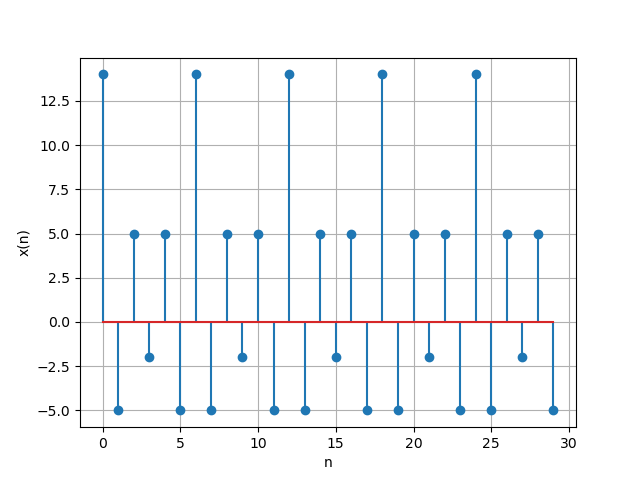
\includegraphics[width=\columnwidth]{2021/EC/39/figs/fig.png}
\caption{\large{STEM PLOT OF $y\brak{n}$}}
\end{figure}


\pagebreak
\item Let $X\brak{j \omega}$ denotes the Fourier transform of $x\brak{t}$. If 
\begin{align}
X\brak{j \omega} =& 10e^{-j\pi f \: \brak{\dfrac{sin\brak{\pi f}}{\pi f}}}
\end{align} 
then $ \dfrac{1}{2\pi} \int_{-\infty }^{\infty} X\brak{j \omega} d\omega = \rule{1cm}{0.15mm}$ .  (where $\omega$ = $2\pi f$)\\
\begin{enumerate}[label = \brak{\Alph*}]
\item 10$\pi$ \\
\item 100 \\
\item 10 \\
\item 20$\pi$ 
\end{enumerate}
\hfill GATE 2021\\
\solution
%\iffalse
\let\negmedspace\undefined
\let\negthickspace\undefined
\documentclass[journal,12pt,twocolumn]{IEEEtran}
\usepackage{cite}
\usepackage{amsmath,amssymb,amsfonts,amsthm}
\usepackage{algorithmic}
\usepackage{graphicx}
\usepackage{textcomp}
\usepackage{xcolor}
\usepackage{txfonts}
\usepackage{listings}
\usepackage{enumitem}
\usepackage{mathtools}
\usepackage{gensymb}
\usepackage{comment}
\usepackage[breaklinks=true]{hyperref}
\usepackage{tkz-euclide} 
\usepackage{listings}
\usepackage{gvv}  
\usepackage{tikz}
\usepackage{circuitikz} 
\usepackage{caption}

\def\inputGnumericTable{}                                
\usepackage[latin1]{inputenc}                 
\usepackage{color}                            
\usepackage{array}                            
\usepackage{longtable}                        
\usepackage{calc}                            
\usepackage{multirow}                      
\usepackage{hhline}                           
\usepackage{ifthen}                          
\usepackage{lscape}
\usepackage{amsmath}
\newtheorem{theorem}{Theorem}[section]
\newtheorem{problem}{Problem}
\newtheorem{proposition}{Proposition}[section]
\newtheorem{lemma}{Lemma}[section]
\newtheorem{corollary}[theorem]{Corollary}
\newtheorem{example}{Example}[section]
\newtheorem{definition}[problem]{Definition}
\newcommand{\BEQA}{\begin{eqnarray}}
\newcommand{\EEQA}{\end{eqnarray}}
\newcommand{\define}{\stackrel{\triangle}{=}}
\theoremstyle{remark}
\newtheorem{rem}{Remark}


\begin{document}
%

\bibliographystyle{IEEEtran}


\vspace{3cm}

\title{
%	\logo{
GATE 2021 BM

\large{EE:1205 Signals and System}

Indian Institute of Technology, Hyderabad
%	}
}
\author{Prashant Maurya

EE23BTECH11218
}	
%\title{
%	\logo{Matrix Analysis through Octave}{\begin{center}\includegraphics[scale=.24]{tlc}\end{center}}{}{HAMDSP}
%}


% paper title
% can use linebreaks \\ within to get better formatting as desired
%\title{Matrix Analysis through Octave}
%
%
% author names and IEEE memberships
% note positions of commas and nonbreaking spaces ( ~ ) LaTeX will not break
% a structure at a ~ so this keeps an author's name from being broken across
% two lines.
% use \thanks{} to gain access to the first footnote area
% a separate \thanks must be used for each paragraph as LaTeX2e's \thanks
% was not built to handle multiple paragraphs
%

%\author{<-this % stops a space
%\thanks{}}
%}
% note the % following the last \IEEEmembership and also \thanks - 
% these prevent an unwanted space from occurring between the last author name
% and the end of the author line. i.e., if you had this:
% 
% \author{....lastname \thanks{...} \thanks{...} }
%                     ^------------^------------^----Do not want these spaces!
%
% a space would be appended to the last name and could cause every name on that
% line to be shifted left slightly. This is one of those "LaTeX things". For
% instance, "\textbf{A} \textbf{B}" will typeset as "A B" not "AB". To get
% "AB" then you have to do: "\textbf{A}\textbf{B}"
% \thanks is no different in this regard, so shield the last } of each \thanks
% that ends a line with a % and do not let a space in before the next \thanks.
% Spaces after \IEEEmembership other than the last one are OK (and needed) as
% you are supposed to have spaces between the names. For what it is worth,
% this is a minor point as most people would not even notice if the said evil
% space somehow managed to creep in.



% The paper headers
%\markboth{Journal of \LaTeX\ Class Files,~Vol.~6, No.~1, January~2007}%
%{Shell \MakeLowercase{\textit{et al.}}: Bare Demo of IEEEtran.cls for Journals}
% The only time the second header will appear is for the odd numbered pages
% after the title page when using the twoside option.
% 
% *** Note that you probably will NOT want to include the author's ***
% *** name in the headers of peer review papers.                   ***
% You can use \ifCLASSOPTIONpeerreview for conditional compilation here if
% you desire.




% If you want to put a publisher's ID mark on the page you can do it like
% this:
%\IEEEpubid{0000--0000/00\$00.00~\copyright~2007 IEEE}
% Remember, if you use this you must call \IEEEpubidadjcol in the second
% column for its text to clear the IEEEpubid mark.



% make the title area
\maketitle

\newpage

%\tableofcontents

\bigskip

\renewcommand{\thefigure}{\arabic{figure}}
\renewcommand{\thetable}{\arabic{table}}
%\renewcommand{\theequation}{\theenumi}

%\begin{abstract}
%%\boldmath
%In this letter, an algorithm for evaluating the exact analytical bit error rate  (BER)  for the piecewise linear (PL) combiner for  multiple relays is presented. Previous results were available only for upto three relays. The algorithm is unique in the sense that  the actual mathematical expressions, that are prohibitively large, need not be explicitly obtained. The diversity gain due to multiple relays is shown through plots of the analytical BER, well supported by simulations. 
%
%\end{abstract}
% IEEEtran.cls defaults to using nonbold math in the Abstract.
% This preserves the distinction between vectors and scalars. However,
% if the journal you are submitting to favors bold math in the abstract,
% then you can use LaTeX's standard command \boldmath at the very start
% of the abstract to achieve this. Many IEEE journals frown on math
% in the abstract anyway.

% Note that keywords are not normally used for peerreview papers.
%\begin{IEEEkeywords}
%Cooperative diversity, decode and forward, piecewise linear
%\end{IEEEkeywords}



% For peer review papers, you can put extra information on the cover
% page as needed:
% \ifCLASSOPTIONpeerreview
% \begin{center} \bfseries EDICS Category: 3-BBND \end{center}
% \fi
%
% For peerreview papers, this IEEEtran command inserts a page break and
% creates the second title. It will be ignored for other modes.
\textbf{Question 5:}Let $X\brak{j \omega}$ denotes the Fourier transform of $x\brak{t}$. If 
\begin{align}
X\brak{j \omega} =& 10e^{-j\pi f \: \brak{\dfrac{sin\brak{\pi f}}{\pi f}}}
\end{align} 
then $ \dfrac{1}{2\pi} \int_{-\infty }^{\infty} X\brak{j \omega} d\omega = \rule{1cm}{0.15mm}$ .  (where $\omega$ = $2\pi f$)\\
\begin{enumerate}[label = \brak{\Alph*}]
\item 10$\pi$ \\
\item 100 \\
\item 10 \\
\item 20$\pi$ 
\end{enumerate}
\hfill GATE 2021\\
\textbf{Solution}  
\begin{align}
\label{eq : 2}A rect \brak{\dfrac{t}{\tau}} \longleftrightarrow A \tau sinc\brak{f\tau} \\
\label{eq : 3}x\brak{t} \longleftrightarrow  X\brak{j \omega} \\
\label{eq : 4}x\brak{t-a} \longleftrightarrow e^{-j \omega \: a}X\brak{j \omega}
\end{align}
\begin{figure}[ht]
	\centering
    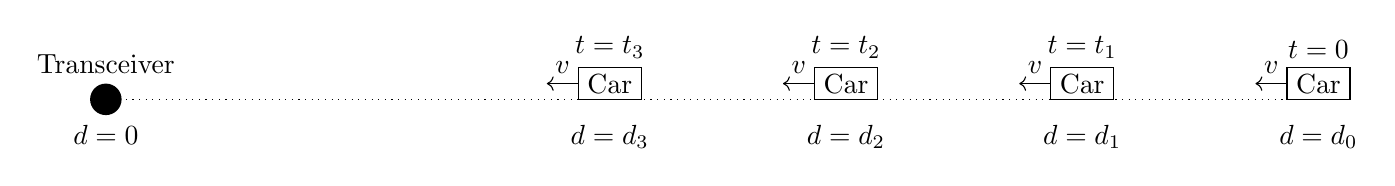
\begin{tikzpicture}

    % Draw the transceiver
    \fill[black] (0,0) circle (0.2) node[above] at (0,0.2) {Transceiver} node[below] at (0,-0.2) {$d=0$};

    % Draw the car at distance D_0
    \draw (15,0) rectangle ++(0.8,0.4) node[midway] {Car} node[above] at (15.4,0.4) {$t=0$ } node[below] at (15.4,-0.2) {$d=d_0$};
    \draw[->] (15,0.2) -- node[above] {$v$} (14.6,0.2);

    \draw (12,0) rectangle ++(0.8,0.4) node[midway] {Car} node[above] at (12.4,0.4) {$t=t_1$ } node[below] at (12.4,-0.2) {$d=d_1$};
    \draw[->] (12,0.2) -- node[above] {$v$} (11.6,0.2);

    \draw (9,0) rectangle ++(0.8,0.4) node[midway] {Car} node[above] at (9.4,0.4) {$t=t_2$ } node[below] at (9.4,-0.2) {$d=d_2$};
    \draw[->] (9,0.2) -- node[above] {$v$} (8.6,0.2);

    \draw (6,0) rectangle ++(0.8,0.4) node[midway] {Car} node[above] at (6.4,0.4) {$t=t_3$ } node[below] at (6.4,-0.2) {$d=d_3$};
    \draw[->] (6,0.2) -- node[above] {$v$} (5.6,0.2);

    \draw[dotted] (0,0) -- (15,0);

\end{tikzpicture}




    \label{fig: 1}
    \caption{}
\end{figure}

From $X\brak{j \omega}$ , we can have $x\brak{t}$ as
\begin{align}
x\brak{t} =& \dfrac{1}{2\pi} \int_{-\infty }^{\infty} X\brak{j \omega} e^{j \omega \: t} d\omega
\end{align}
For $t=0$ ,
\begin{align}
x\brak{0} =& \dfrac{1}{2\pi} \int_{-\infty }^{\infty} X\brak{j \omega} d\omega
\end{align}
On comparing , we get $A = 10$ and $ \tau = 1$,
\begin{align}
10 rect \brak{t} \longleftrightarrow 10  sinc\brak{f} 
\end{align}
\begin{figure}[ht]
	\centering
    \begin{figure}[!h]
    \centering
    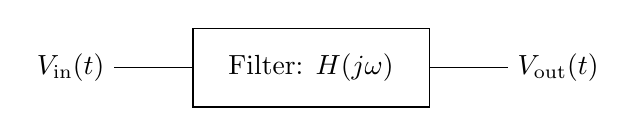
\begin{tikzpicture}
    % Draw the filter rectangle
    \draw (0,0) rectangle (3,1) node[midway] {Filter: $H(j\omega)$};
    
    % Draw the input and output labels
    \draw (-1,0.5) node[left] {$V_{\text{in}}(t)$} -- (0,0.5);
    \draw (3,0.5) -- (4,0.5) node[right] {$V_{\text{out}}(t)$};
\end{tikzpicture}
    \caption{Filter Equivalent of Circuit}
    \label{fig:2_gate.22.ee.31}
\end{figure}
    \label{fig: 2}
    \caption{}
\end{figure}
\begin{align}
10 rect \brak{t-\dfrac{1}{2}} \longleftrightarrow 10e^{-j2\pi f \times \dfrac{1}{2}}sinc \brak{f}
\end{align}
\begin{figure}[ht]
	\centering
    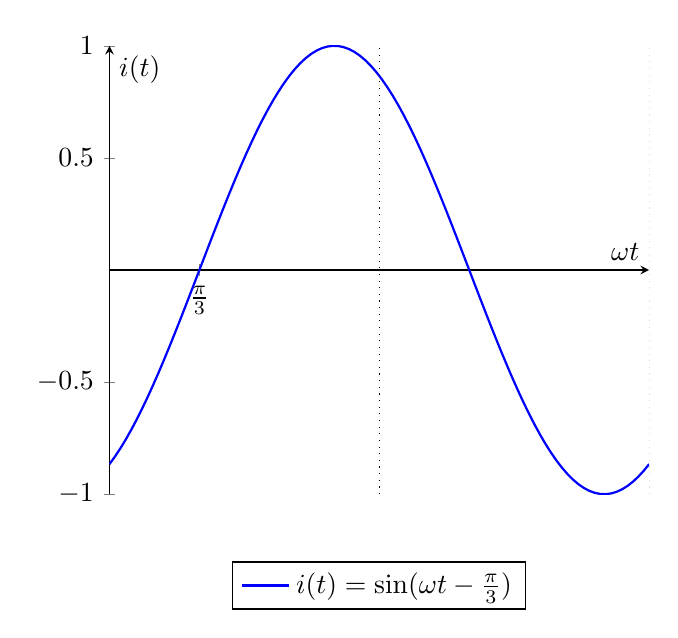
\begin{tikzpicture}

% Adjust the domain and samples according to your preference
\begin{axis}[
    xlabel={$\omega t$},
    ylabel={$i(t)$},
    domain=0:2*pi,
    samples=100,
    axis lines=middle,
    xtick={pi/3}, % Set x-axis tick at pi/3
    xticklabels={$\frac{\pi}{3}$}, % Label for the tick
    ytick={}, % Remove y-axis ticks
    legend style={at={(0.5,-0.15)},anchor=north},
]

% Plot the function
\addplot[blue,thick] {sin(deg(x - pi/3))};
\addlegendentry{$i(t) = \sin(\omega t - \frac{\pi}{3})$}

% Dotted vertical lines at x=pi and x=2pi
\draw[dotted] (axis cs:pi, \pgfkeysvalueof{/pgfplots/ymin}) -- (axis cs:pi, \pgfkeysvalueof{/pgfplots/ymax});
\draw[dotted] (axis cs:2*pi, \pgfkeysvalueof{/pgfplots/ymin}) -- (axis cs:2*pi, \pgfkeysvalueof{/pgfplots/ymax});

\end{axis}

\end{tikzpicture}

    \label{fig: 3}
    \caption{}
\end{figure}

From the above figure, $x\brak{0}$ is 10.\\
Hence, the correct option is \brak{C}.
\end{document}
\item Consider the sequence $ x_n = 0.5x_{n-1} + 1 , n = 1,2,...$ with $x_0 = 0$ Then $ \lim_{n \to \infty} x_n$ is :
\begin{enumerate}
\item[A]0
\item[B]1
\item[C]2
\item[D]$\infty$
\end{enumerate}
\hfill {GATE 2021 IN}\\
\solution
\iffalse
\let\negmedspace\undefined
\let\negthickspace\undefined
\documentclass[journal,12pt,onecolumn]{IEEEtran}
\usepackage{cite}
\usepackage{amsmath,amssymb,amsfonts,amsthm}

\usepackage{graphicx}
\usepackage{textcomp}
\usepackage{xcolor}
\usepackage{txfonts}
\usepackage{listings}
\usepackage{enumitem}
\usepackage{mathtools}
\usepackage{gensymb}
\usepackage[breaklinks=true]{hyperref}
\usepackage{tkz-euclide} % loads  TikZ and tkz-base
\usepackage{listings}
\usepackage{gvv}
\usepackage{booktabs}

%
%\usepackage{setspace}
%\usepackage{gensymb}
%\doublespacing
%\singlespacing

%\usepackage{graphicx}
%\usepackage{amssymb}
%\usepackage{relsize}
%\usepackage[cmex10]{amsmath}
%\usepackage{amsthm}
%\interdisplaylinepenalty=2500
%\savesymbol{iint}
%\usepackage{txfonts}
%\restoresymbol{TXF}{iint}
%\usepackage{wasysym}
%\usepackage{amsthm}
%\usepackage{iithtlc}
%\usepackage{mathrsfs}
%\usepackage{txfonts}
%\usepackage{stfloats}
%\usepackage{bm}
%\usepackage{cite}
%\usepackage{cases}
%\usepackage{subfig}
%\usepackage{xtab}
%\usepackage{longtable}
%\usepackage{multirow}

%\usepackage{algpseudocode}
%\usepackage{enumitem}
%\usepackage{mathtools}
%\usepackage{tikz}
%\usepackage{circuitikz}
%\usepackage{verbatim}
%\usepackage{tfrupee}
%\usepackage{stmaryrd}
%\usetkzobj{all}
%    \usepackage{color}                                            %%
%    \usepackage{array}                                            %%
%    \usepackage{longtable}                                        %%
%    \usepackage{calc}                                             %%
%    \usepackage{multirow}                                         %%
%    \usepackage{hhline}                                           %%
%    \usepackage{ifthen}                                           %%
  %optionally (for landscape tables embedded in another document): %%
%    \usepackage{lscape}     
%\usepackage{multicol}
%\usepackage{chngcntr}
%\usepackage{enumerate}

%\usepackage{wasysym}
%\documentclass[conference]{IEEEtran}
%\IEEEoverridecommandlockouts
% The preceding line is only needed to identify funding in the first footnote. If that is unneeded, please comment it out.

\newtheorem{theorem}{Theorem}[section]
\newtheorem{problem}{Problem}
\newtheorem{proposition}{Proposition}[section]
\newtheorem{lemma}{Lemma}[section]
\newtheorem{corollary}[theorem]{Corollary}
\newtheorem{example}{Example}[section]
\newtheorem{definition}[problem]{Definition}
%\newtheorem{thm}{Theorem}[section] 
%\newtheorem{defn}[thm]{Definition}
%\newtheorem{algorithm}{Algorithm}[section]
%\newtheorem{cor}{Corollary}
\newcommand{\BEQA}{\begin{eqnarray}}
\newcommand{\EEQA}{\end{eqnarray}}
\newcommand{\define}{\stackrel{\triangle}{=}}
\theoremstyle{remark}
\newtheorem{rem}{Remark}

%\bibliographystyle{ieeetr}
\begin{document}
%

\bibliographystyle{IEEEtran}


\vspace{3cm}

\title{
%	\logo{
Gate 2021 Assignment 

\large{EE:1205 Signals and Systems}

Indian Institute of Technology, Hyderabad
%	}
}
\author{Abhey Garg

EE23BTECH11202
}	


% make the title area
\maketitle



%\tableofcontents


\renewcommand{\thefigure}{\theenumi}
\renewcommand{\thetable}{\theenumi}
%\renewcommand{\theequation}{\theenumi}

\section{Question IN 02}
Consider the sequence $ x_n = 0.5x_{n-1} + 1 , n = 1,2,...$ with $x_0 = 0$ Then $ \lim_{n \to \infty} x_n$ is :
\begin{enumerate}
\item[A]0
\item[B]1
\item[C]2
\item[D]$\infty$
\end{enumerate}
\section{Solution}
\fi
\begin{align}
x_n = 0.5 x_{n-1} + 1
\end{align}
Taking Z-transform:
\begin{align}
X(z) = 0.5 z^{-1} X(z) + \frac{1}{1-z^{-1}} \\
X(z)[1-0.5z^{-1}] = \frac{1}{1-z^{-1}} \\
X(z) = \frac{1}{(1-z^{-1})(1-0.5z^{-1})}\\
X(z) = \frac{A}{1-z^{-1}} + \frac{B}{1-0.5z^{-1}}\\
A+B = 1 \\
A = -2B \\
A = 2 \\
B = -1 \\
X(z) = \frac{2}{1-z^{-1}} + \frac{-1}{1-0.5z^{-1}}\\
\end{align}
Taking inverse Z-transform:
\begin{align}
x(n) = 2 u(n) + (-1)(0.5^n)u(n)\\
\lim_{n \to \infty} x(n) = 2
\end{align}

%\end{document}

\end{enumerate}

  \chapter{Numerical Methods}
 \section{2022}
 \begin{enumerate}[label=\thechapter.\arabic*,ref=\thechapter.\theenumi]
\item
\solution
\input{}
\pagebreak
\end{enumerate}

 \section{2021}
 \begin{enumerate}[label=\thechapter.\arabic*,ref=\thechapter.\theenumi]
\item An ordinary differential equation (ODE) $\frac{dy}{dx} = 2y$ with an initial condition $y(0) = 1$ has the analytical
solution $y = e^{2x}$
 Using Runge-Kutta second order method, numerically integrate the ODE to calculate $y$ at $x = 0.5$ using a
step size of $h = 0.5$.
 If the relative percentage error is defined as 
 \begin{align}
 \epsilon = \left|\frac{y_{analytical} - y_{numerical}}{y_{analytical}}\right| \times 100 \nonumber
 \end{align}
 then the value of $\epsilon$ at $x = 0.5$ is
 
\hfill(GATE 1 CH 2021)
\solution
 \iffalse
\let\negmedspace\undefined
\let\negthickspace\undefined
\documentclass[journal,12pt,twocolumn]{IEEEtran}
\usepackage{cite}
\usepackage{amsmath,amssymb,amsfonts,amsthm}
\usepackage{algorithmic}
\usepackage{graphicx}
\usepackage{textcomp}
\usepackage{xcolor}
\usepackage{txfonts}
\usepackage{listings}
\usepackage{enumitem}
\usepackage{mathtools}
\usepackage{gensymb}
\usepackage{comment}
\usepackage[breaklinks=true]{hyperref}
\usepackage{tkz-euclide} 
\usepackage{tikz}
\usepackage{circuitikz}
\usepackage{listings}
\usepackage{gvv}                                        
\def\inputGnumericTable{}                                 
\usepackage[latin1]{inputenc}                                
\usepackage{color}                                            
\usepackage{array}                                            
\usepackage{longtable}                                       
\usepackage{calc}                                             
\usepackage{multirow}                                         
\usepackage{hhline}                                           
\usepackage{ifthen}                                           
\usepackage{lscape}
\usepackage{caption}
\newtheorem{theorem}{Theorem}[section]
\newtheorem{problem}{Problem}
\newtheorem{proposition}{Proposition}[section]
\newtheorem{lemma}{Lemma}[section]
\newtheorem{corollary}[theorem]{Corollary}
\newtheorem{example}{Example}[section]
\newtheorem{definition}[problem]{Definition}
\newcommand{\BEQA}{\begin{eqnarray}}
\newcommand{\EEQA}{\end{eqnarray}}
\newcommand{\define}{\stackrel{\triangle}{=}}
\theoremstyle{remark}
\newtheorem{rem}{Remark}
\begin{document}
\parindent 0px
\bibliographystyle{IEEEtran}
\vspace{3cm}

\title{GATE 2021 1.CH}
\author{EE23BTECH11012 - Chavan Dinesh$^{*}$% <-this % stops a space
}
\maketitle
\newpage
\bigskip

\renewcommand{\thefigure}{\arabic{figure}}
\renewcommand{\thetable}{\arabic{table}}
\large\textbf{\textsl{Question:}}
An ordinary differential equation (ODE) $\frac{dy}{dx} = 2y$ with an initial condition $y(0) = 1$ has the analytical
solution $y = e^{2x}$
 Using Runge-Kutta second order method, numerically integrate the ODE to calculate $y$ at $x = 0.5$ using a
step size of $h = 0.5$.
 If the relative percentage error is defined as 
 \begin{align}
 \epsilon = \left|\frac{y_{analytical} - y_{numerical}}{y_{analytical}}\right| \times 100 \nonumber
 \end{align}
 then the value of $\epsilon$ at $x = 0.5$ is
 
\hfill(GATE 1 CH 2021)

\solution
\fi
\begin{table}[htbp]
    \centering
        \begin{tabular}{|c|c|}
        \hline
        \textbf{Constant} & \textbf{Description} \\
        \hline
        $y(0.5)$ & $y_{analytical}$\\
        \hline
        $y_1$ & $y_{numerical}$ \\
        \hline
        $\frac{dy}{dx}=f(x, y)$ & Function representing the ODE\\
        \hline
        $h$ & Step size \\
        \hline
        $K_1$ & First slope estimate in the Runge-Kutta \\
        \hline
        $K_2$ & Second slope estimate in the Runge-Kutta \\
        \hline
        $K$ & Weighted average of $K_1$ and $K_2$ \\
        \hline
    \end{tabular}


    \caption{}
    \label{tab:input_parameters.1.BM.2021}
\end{table}

Analytical solution is given by:
\begin{align}
    y = e^{2x}
\end{align}
At $x = 0.5$, analytical solution is 
\begin{align}
    y(0.5) = e^{2\times 0.5} = 2.718 
\end{align}
According to question:
\begin{align}
    f(x,y) = \frac{dy}{dx} = 2y
\end{align}
By Runge-kutta $2^{nd}$ order method, 
\begin{align}
    K_1 = hf(x_o,y_o) = h(2y_o)\\
    K_1 = 0.5(2 \times 1) = 1
\end{align}
\begin{align}
    K_2 = h[f(x_o + h, y_o + K_1)]\\
    K_2 = h[2(1 +1)]\\
    K_2 = 0.5 \times 4 = 2 
\end{align}
\begin{align}
    K = \frac{K_1 + K_2}{2} = \frac{1 +2}{2} = 1.5
\end{align}
\begin{align}
    y_{_{1}} = y_{numerical} = y_o + K = 1 + 1.5 = 2.5 
\end{align}
Hence, 
\begin{align}
    \epsilon = \left|\frac{2.718 - 2.5}{2.718}\right| \times 100 \\
    \epsilon = \frac{0.218}{2.718}\times 100 = 8\%
 \end{align}
% \begin{figure}[ht]
%     \centering
%     \includegraphics[width = \columnwidth]{figs/x_n_stem_plot.png}
%     \caption{}
%     \label{fig:graph1.11.9.3.28}
% \end{figure}

\bibliographystyle{IEEEtran}

\pagebreak
\end{enumerate}

\backmatter
\appendix
\chapter{Fourier transform}
\begin{enumerate}[label=\thechapter.\arabic*,ref=\thechapter.\theenumi]
\numberwithin{equation}{enumi}
\numberwithin{figure}{enumi}
\numberwithin{table}{enumi}
\item The Differentiation in frequency domain is as follows\\
        Let x(t) be a signal such that,
    \begin{align}
        x\brak{t}&\xleftrightarrow{\text{F.T}} X\brak{\omega}\\
        X\brak{\omega}&=\int_{t=-\infty}^{\infty}x\brak{t}e^{-j\omega t}dt\\
        \frac{d}{d\omega}X\brak{\omega}&=\int_{t=-\infty}^{\infty}x\brak{t}\brak{-jt}e^{-j\omega t}dt\\
        j\frac{d}{d\omega}X\brak{\omega}&=\int_{t=-\infty}^{\infty}tx\brak{t}e^{-j\omega t}dt\\
        tx\brak{t}&\xleftrightarrow{\text{F.T}} j\frac{d}{d\omega}X\brak{\omega}\label{eq:Differentiation-property}
    \end{align}
\item The duality property is as follows\\
    From inverse Fourier transform we get,
    \begin{align}
        x\brak{t}&=\frac{1}{2\pi}\int_{-\infty}^{\infty}X\brak{\omega}e^{j\omega t}d\omega
    \end{align}
    Replacing t by -t and multiplying 2$\pi$ on both sides we get,
    \begin{align}
        2\pi x\brak{-t}&=\int_{-\infty}^{\infty}X\brak{\omega}e^{-j\omega t}d\omega\\
        X\brak{t}&\xleftrightarrow{\text{F.T}} 2\pi x\brak{-\omega}\label{eq:Duality-property}
    \end{align}
    
\item Complex Fourier Series	\\
\begin{align}
	x(t) &= \sum_{n=-\infty}^{\infty} c_{n}e^{j2\pi nft}
	\label{eq:compfs}
\end{align}
where $c_{n}$ is the exponential fourier coefficient.
\begin{align}
        c_{n} &= \frac{1}{T} \int_{0}^{T} x(t) e^{-j2\pi nft} \, dt
\end{align}
where $T$ is the time period of function $x(t)$.
\item Trigonometric Fourier Series	\\
\begin{align}
	e^{j2\pi nft} = cos(2\pi nft ) + j sin(2\pi nft)
	\label{eq:expfs}
\end{align}
Substituting \eqref{eq:expfs} in \eqref{eq:compfs}
\begin{align}
	 x(t) &= \sum_{n=-\infty}^{\infty} c_{n} \brak{\cos(2\pi nft) + j \sin(2\pi nft)}\\
	      &= a_0 + \sum_{n=1}^{\infty} \brak{a_{n} \cos(2\pi nft)} + \brak{b_{n} \sin(2\pi nft)}
\end{align}
where $a_0, a_{n}$ and $b_{n}$ are trigonometric fourier series.
\begin{align}
          a_{0} &= c_{0}\\
                &=\frac{1}{T} \int_{0}^{T} x(t) \, dt\\
          a_{n} &= 2Re(c_{n})\\
                &=\frac{2}{T} \int_{0}^{T} x(t)\cos(2\pi nft) \, dt\\
          b_{n} &= -2Im(c_{n})\\
                &= \frac{2}{T} \int_{0}^{T} x(t)\sin(2\pi nft) \, dt
\end{align}

\item Peridicity of Fourier coefficients\\
For a signal $x[n] = \sum_{k=0}^{N-1}a_ke^{j\brak{\frac{2kn\pi}{N}}}$, defining $X[k] = Na_k$.
\begin{align}
x[n] &= \frac{1}{N}\sum_{k=0}^{N-1}X[k]e^{j\brak{\frac{2kn\pi}{N}}}\\
\sum_{n=0}^{N-1}x[n]e^{-j\brak{\frac{2rn\pi}{N}}} &= \sum_{n=0}^{N-1}\frac{1}{N}\sum_{k=0}^{N-1}X[k]e^{j\brak{\frac{2kn\pi}{N}}}e^{-j\brak{\frac{2rn\pi}{N}}}\\
&= \sum_{k=0}^{N-1}X[k]\sum_{n=0}^{N-1}\frac{1}{N}e^{j\brak{\frac{2\brak{k-r}n\pi}{N}}}\\
\sum_{n=0}^{N-1}\frac{1}{N}e^{j\brak{\frac{2\brak{k-r}n\pi}{N}}}&=\begin{cases}
1 & k-r=mN, m \in \mathbb{Z}\\
0 & \text{ otherwise}
\end{cases}\\
\implies X[k] &= \sum_{n=0}^{N-1}x[n]e^{-j\brak{\frac{2kn\pi}{N}}} \label{X[k]_F_coeff}
\end{align}
If $x[n] = x[n+rN],r \in \mathbb{Z}$, from \eqref{X[k]_F_coeff},
\begin{align}
X[k+rN] &= \sum_{n=0}^{N-1}x[n]e^{-j\brak{\frac{2\brak{k+rN}n\pi}{N}}}\\
&= \sum_{n=0}^{N-1}x[n]e^{-j\brak{\frac{2kn\pi}{N}}}e^{-j\brak{2rn\pi}}\\
&= \sum_{n=0}^{N-1}x[n]e^{-j\brak{\frac{2kn\pi}{N}}}\\
&= X[k]\\
\implies a_k &= a_{k+rN},r \in \mathbb{Z} \label{a_k=a_{k+rN}}
\end{align}
\end{enumerate}

\chapter{Contour Integration}
\begin{enumerate}[label=\thechapter.\arabic*,ref=\thechapter.\theenumi]
\numberwithin{equation}{enumi}
\numberwithin{figure}{enumi}
\numberwithin{table}{enumi}
\item Cauchy's Theorem: \label{Cauchy} \\
From Figure \ref{fig:fig1_Cauchy}
\begin{align}
    \int_C f\brak{z}dz &= \int_{Cr} f\brak{z}dz
\end{align}
\begin{figure}[ht]
    \centering
    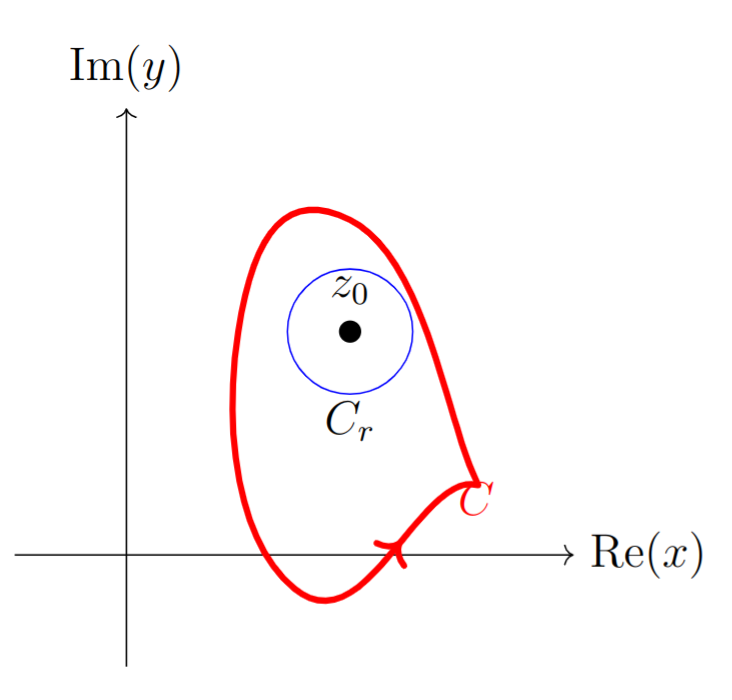
\includegraphics[width=0.5\textwidth]{app/figs/img1.png}
    \caption{Figure1}
    \label{fig:fig1_Cauchy}
\end{figure}
Since  $g\brak{z}$ is continuous we know that $\abs{g\brak{z}}$ is bounded inside  $C_r$. Say,  $\abs{g\brak{z}}<M$. The corollary to the triangle inequality says that
\begin{align}
    \abs{\int_{C_r}f\brak{z}\, dz} &\leq M2\pi r.
\end{align}
Since  $r$ can be as small as we want, this implies that
\begin{align}
    \int_{Cr} f\brak{z}dz &= 0
\end{align}
let \begin{align}
    g\brak{z} &= \frac{f\brak{z} - f\brak{z_0}}{z-z_0}\\
    \lim_{z \to z_0} g(z) &= f'(z_0)\\
    \int_{C} g(z)\ dz = 0, &\implies \int_C \frac{f(z) - f(z_0)}{z - z_0} \ dz = 0
\end{align}
Thus,
\begin{align}
    \int_{C} \frac{f(z)}{z - z_0}\ dz = \int_C \dfrac{f(z_0)}{z - z_0}\ dz = 2\pi i f(z_0) \label{eq:eq3_gate_2022_ma_14}
\end{align}

Using Cauchy's Theorem,
\begin{align}
    \int_C f\brak{z} &= 0\\
    f\brak{a} &= \frac{1}{2 \pi i}\oint_C\frac{f\brak{z}}{z-a}\, dz\\
    f^{n}\brak{a} &= \frac{n!}{2 \pi i}\oint_C\frac{f\brak{z}}{\brak{z-a}^{n+1}}\, dz
\end{align}
\pagebreak
\item Residue Theorem:\label{Residue} \\
From eq (\ref{eq:eq3_gate_2022_ma_14})
\begin{align}
    \int_C f\brak{z}\, dz &= 2 \pi i \sum{Res \, f\brak{a}} \label{eq:eq1_gate_ma_2022_14_054}
\end{align}
where, for n repeated poles,
\begin{align}
    Res \, f\brak{a} &= \lim_{z \to a}\frac{1}{\brak{n-1}!}\brak{\frac{d^{n-1}}{dz^{n-1}}\sbrak{\brak{z-a}^n\, f\brak{z}}} \label{eq:eq2_gate_ma_2022_14_054}
\end{align}
\end{enumerate}

\chapter{Laplace Transform}
\begin{enumerate}[label=\thechapter.\arabic*,ref=\thechapter.\theenumi]
\numberwithin{equation}{enumi}
\numberwithin{figure}{enumi}
\numberwithin{table}{enumi}
\item Laplace Transform of Partial Differentials\\
Let a function $y\brak{x,t}$ be defined for all $t>0$ and assumed to be bounded. Appling Laplace transform in t considering x as a parameter,
\begin{align}
 \mathcal{L}\brak{y\brak{x,t}} &= \int_{0}^{\infty}e^{-st}y\brak{x,t}dt\\
 &= Y\brak{x,s}
\end{align}
Let $\dfrac{\partial y\brak{x,t}}{\partial t}$ be $y_t\brak{x,t}$ and $\dfrac{\partial y\brak{x,t}}{\partial x}$ be $y_x\brak{x,t}$, then
\begin{align}
 \mathcal{L}\brak{y_t\brak{x,t}} &= \int_{0}^{\infty}e^{-st}y_t\brak{x,t}dt\\
 &= \left. e^{-st}y\brak{x,t}\right|_{0}^{\infty} + s\int_{0}^{\infty}e^{-st} y\brak{x,t} dt\\
 &= sY\brak{x,s} - y\brak{x,0} \label{L(y_t(x,t))}\\
 \mathcal{L}\brak{y_x\brak{x,t}} &= \int_{0}^{\infty}e^{-st}y_x\brak{x,t}dt\\
 &= \dfrac{d}{dx}\int_{0}^{\infty}e^{-st}y\brak{x,t}dt \label{L(y_x(x,t))}\\
 &= \dfrac{dY\brak{x,s}}{dx}
\end{align}
\item Laplace transform of f(t):
\begin{align}
        f(t)u(t)\system{L}&\int_{0}^{\infty}f(t)e^{-st}\; dt\\
        &=F(s)\label{lap transform}
\end{align}
\item Laplace transform of powers of $t$\\
        Let $f(t)=t^nu(t)$\\
From \eqref{lap transform},and considering $h=st$
\begin{align}
        F(s)&=\frac{1}{s^{n+1}}\int_{0}^{\infty}h^ne^{-h}\;dh\label{lap 1}\\
        (n-1)!&=\int_0^\infty e^{-t}t^{n-1}\;dt\text{ (Gamma function)}\label{gamma}
\end{align}
From \eqref{lap 1},\eqref{gamma}
\begin{align}
        F(s)&=\frac{n!}{s^{n+1}}\\
         t^nu(t)&\system{L}\frac{n!}{s^{n+1}}\label{lap exp}
\end{align}
\item Frequency shift property:\\
        Let $f(t)=y(t)e^{-at}u(t)$\\
From\eqref{lap transform},
\begin{align}
        F(s)&=\int_0^{\infty}y(t)e^{-(s+a)t}\;dt\\
         y(t)e^{-at}u(t)&\system{L}Y(s+a)\label{lap freq shift}
\end{align}
\item Inverse Laplace for partial fractions\\
From \eqref{lap exp},\eqref{lap freq shift} we get
\begin{align}
    &\frac{b}{(s+a)^n}\xleftrightarrow{\mathcal{L}^{-1}}\frac{b}{(n-1)!}\cdot t^{n-1} e^{-at}\cdot u(t)\label{inv lap (partial fractions)}
\end{align}
\item Laplace transform of derivatives:\\
        Let $f(t)=y'(t)u(t)$\\
From \eqref{lap transform}, integration by parts,recursion
\begin{align}
        F(s)&=\int_{0}^\infty e^{-st}\; dy\\
        &=[y(t)e^{-st}]_0^\infty+s\int_0^\infty y(t)e^{-st}dt\\
        &=-y(0)+sY(s)\label{lap 2}
\end{align}
From\eqref{lap 2},recursion
\begin{align}
        y'(t)u(t)&\system{L}sY(s)-\int y'(t)\;dt\vert_{t=0}\\
        y^{(n)}(t)u(t)&\system{L}s^nY(s)-\sum\limits_{k=0}^{n-1}s^{(n-1-k)}y^{(k)}(0)\label{lap (derivatives)}
\end{align}

\item Laplace transform of integrals:\\
Let the function defined as $y(t) = \int_0^t f(u) du$ for all $t > 0$\\
Laplace transform of y(t) in t 
\begin{align}
    \mathcal{L} \brak{y(t)} &= \int_0^{\infty} e^{-st} y(t) dt\\
    &= \int_0^{\infty} e^{-st} \int_0^t f(u) du dt\\
    &= \int_0^t f(u) du \sbrak{- \frac{e^{-st}}{s}}_0^{\infty} + \int_0^{\infty} \frac{e^{-st}}{s} f(t) dt\\
    &= \frac{F(s)}{s}
\end{align}


\end{enumerate}

\chapter{Filters}
\begin{enumerate}[label=\thechapter.\arabic*,ref=\thechapter.\theenumi]
\numberwithin{equation}{enumi}
\numberwithin{figure}{enumi}
\numberwithin{table}{enumi}

\item \begin{figure}[!ht]
    \centering
    \begin{circuitikz}
   \draw(0,0) to [R](2,0);
   % \draw (2,0) -- (2.5,0);
   \draw(2,0) to [L] (4,0);
   % \draw (5,0) to (5,0);
   \draw (4,0) to [C] (4,-2);
   \draw(4,-2)  to (0,-2);
   \draw (4,0) -- (5,0);
   \draw (4,-2)to (5,-2);
   \node[circle,fill,inner sep=1pt] at (0,0) {};
   \node[circle,fill,inner sep=1pt] at (5,0) {};
   \node[circle,fill,inner sep=1pt] at (5,-2) {};
   \node[circle,fill,inner sep=1pt] at (0,-2) {};
   \draw[->](0,-1.85) to (0,-0.15);
   \draw[->](5,-1.85) to (5,-0.15);
   \node at (0.3,-1) {$x(t)$};
   \node at (5.5,-1) {$y(t)$};

   \node at (1,0.5) {$R$};
   \node at (3,0.5) {$L$};
   \node at (2.8,-1) {$C$};\node[circle,fill,inner sep=1pt] at (0,0) {};
\end{circuitikz}

    \caption{RLC Low pass filter}
\end{figure}
\begin{table}[!ht]
    \centering
    \begin{tabular}{|c|c|}
\hline
    \textbf{Parameter} & \textbf{Description}  \\
    \hline
    $Z_C$ & Reactance of Capacitor \\
    \hline
    $Z_R$ & Reactance of Resistor \\
    \hline
    $Z_L$ & Recatance of Inductor \\
    \hline
    $x(t) = u(t)$ & Input Response \\
    \hline
    $y(t)$ & Output across capacitor \\
    \hline
    $\omega_0$ & Angular resonant frequency \\
    \hline
    \end{tabular}

    \caption{Input Parameters}
\end{table}
\begin{align}
    Y(s) &= I(s)Z_C\\
    &= \frac{X(s)}{Z_L + Z_R + Z_C}Z_C\\
    H(s) &= \frac{Y(s)}{X(s)}\\
    &= \frac{Z_C}{Z_L + Z_R + Z_C}\\
    &= \frac{\frac{1}{sC}}{sL + R + \frac{1}{sC}}\\
    &= \frac{1}{s^2LC + sRC + 1}\\
    \implies H(s) &= \omega_0^2\frac{1}{(s-p_1)(s-p_2)}
\end{align}
where,
\begin{align}
    \omega_0 &= \frac{1}{\sqrt{LC}}\\
    p_{1, 2} &= -\frac{R}{2L} \pm \sqrt{\brak{\frac{R}{2L}}^2 - \frac{1}{LC}}\\
    &= -\alpha \pm \sqrt{\alpha^2 - \omega_0^2}
\end{align}
where
\begin{align}
    \alpha &= \frac{R}{2L}
\end{align}
Damping Factor is given by,
\begin{align}
   \zeta &= \frac{\alpha}{\omega_0}\\
   &= \frac{R}{2}\sqrt{\frac{C}{L}}
\end{align}
\begin{table}[!ht]
    \centering
    \begin{tabular}{|c|c|c|c|}
\hline
    $\zeta$ & \textbf{Pole Location} & \textbf{Referred to as} & \textbf{Condition} \\
    \hline
    $\zeta > 1$ & Different locations on&&\\& the negative real axis & Overdamped & $R > 2\sqrt{\frac{L}{C}}$\\
    \hline
    $\zeta = 1$ & Coincide on&&\\& the negative real axis & Critically Damped & $R = 2\sqrt{\frac{L}{C}}$\\
    \hline
    $\zeta < 1$ & Complex Conjugate poles in&&\\& the left half of s-plane & Underdamped & $R < 2\sqrt{\frac{L}{C}}$\\
    \hline
\end{tabular}

    \caption{Effect of Damping Coefficient $\zeta$ on system behaviour}
\end{table}
\newpage
\begin{enumerate}
\item Overdamped Response
\begin{align}
    Y(s) &= X(s)H(s)\\
    &= \omega_0^2\frac{1}{s(s-p_1)(s-p_2)}\\
    &= \frac{c_0}{s} + \frac{c_1}{s-p_1} + \frac{c_2}{s-p_2}
\end{align}
where,
\begin{align}
    c_0 &= 1\\
    c_1 &= \frac{p_2}{p_1 - p_2}\\
    c_2 &= \frac{p_1}{p_2 - p_1}
\end{align}
Taking inverse Laplace,
\begin{align}
    y(t) &= c_0 + c_1e^{p_1t} + c_2e^{p_2t}\\
    &= \brak{1 + \frac{p_2}{p_1 - p_2}e^{p_1t} +  \frac{p_1}{p_2 - p_1}e^{p_2t}}u(t)
\end{align}

\begin{figure}[!ht]
    \centering
    \begin{tikzpicture}
      \draw[<->] (-4,0) -- (1,0) node[right] {$\mathcal{R}(s)$};
    \draw[<->] (0,-2) -- (0,2) node[above] {$\mathcal{I}(s)$};
  \draw[orange,thick] (-2.1,0.1) -- (-1.9,-0.1);
  \draw[orange,thick] (-2.1,-0.1) -- (-1.9,0.1);
  \draw[orange,thick] (-3.1,0.1) -- (-2.9,-0.1);
  \draw[orange,thick] (-3.1,-0.1) -- (-2.9,0.1);
  \node at (-3,-0.4) {\small $P_1$};
  \node at (-2,-0.4) {\small $P_2$};
\end{tikzpicture}

    \caption{s-Plane for Overdamped case}
\end{figure}

\item Critically Damped Response
\begin{align}
    Y(s)&=X(s)H(s)\\
    &= \omega_0^2\frac{1}{s(s-p)^2}\\
    &= \frac{c_0}{s}+\frac{c_1}{\left(s-p\right)^2}+\frac{c_2}{s-p}
\end{align}
where,
\begin{align}
    c_0 &= 1\\
    c_1 &= p\\
    c_2 &= -1
\end{align}
Taking Inverse Laplace,
\begin{align}
    y(t) &= c_0+(c_1t+c_2)e^{pt}\\
    &= \brak{1+(pt-1)e^{pt}}u(t)
\end{align}
\begin{figure}[!ht]
    \centering
    \begin{tikzpicture}
      \draw[<->] (-4,0) -- (1,0) node[right] {$\mathcal{R}(s)$};
    \draw[<->] (0,-2) -- (0,2) node[above] {$\mathcal{I}(s)$};
  \draw[orange,thick] (-2.1,0.1) -- (-1.9,-0.1);
  \draw[orange,thick] (-2.1,-0.1) -- (-1.9,0.1);
  % \node at (-3,-0.4) {\small $P_1$};
  \node at (-2,-0.4) {\small $p$};
\end{tikzpicture}

    \caption{s-Plane for Critically damped case}
\end{figure}

\item Underdamped Response
\begin{align}
    Y(s) &= X(s)H(s)\\
    &= \omega_0^2\frac{1}{s(s-p)(s-p^\ast)}\\
    &= \frac{c_0}{s}+\frac{c_1}{s-p}+\frac{c_2}{s-p^\ast}
\end{align}
where,
\begin{align}
    c_0 &= 1\\
    c_1 &= \frac{p^\ast}{p-p^\ast}\\
    c_2 &= \frac{p}{p^\ast-p}
\end{align}
Taking Inverse Laplace,
\begin{align}
    y(t) &= c_0+c_1e^{pt}+c_2e^{p^\ast t}\\
    &= 1+\frac{\abs{p}}{\omega_d}\ e^{-\sigma t}\frac{
    e^{j(\omega_d t+\varphi)}+e^{-j(\omega_d t+\varphi)}}{2}\\
    &= \brak{1+\frac{|p|}{\omega_d}e^{-\sigma t}\cos(\omega_d t+\varphi)}u(t)
\end{align}
where,
\begin{align}
    \abs{p}&=\sqrt{{\omega_d}^2+\sigma^2}\\
    \omega_d&=\omega_0\sqrt{1-\zeta^2}\\
    \sigma&=\omega_0\zeta\\
    \varphi&=\pi-\tan^{-1}\frac{\sigma}{\omega_d}
\end{align}
\begin{figure}[!ht]
    \centering
    \begin{tikzpicture}
    \draw[<->] (-4,0) -- (2,0) node[right] {$\mathcal{R}(s)$};
    \draw[<->] (0,-3) -- (0,3) node[above] {$\mathcal{I}(s)$};
       % \draw[blue, thick, ->] (-2,1) -- (0,2);
       %  \draw[blue, thick, ->] (-2,-1) -- (0,2);

  \draw [blue,arrows = {-Latex[width=0pt 10, length=10pt]}] (-2,1) -- (0,2);
   \draw [blue,arrows = {-Latex[width=0pt 10, length=10pt]}] (-2,-1) -- (0,2);

   \draw[brown, dashed] (-2,1) -- (0,1);
   \draw[brown, dashed] (-2,1) -- (-2,-1);
   \draw[brown, dashed] (-2,-1) -- (0,-1);
   \draw[red, dashed] (-2,1) -- (0,0);

   \node at (-2.2,1) {\small$P_{_1}$};
   \node at (-2.2,-1) {\small$P^*$};
   \node [orange]at (-1.7,0.2) {\small$-\sigma$};
   \node[blue] at (0.3,2) {\small $j\omega$};
    \node[brown] at (0.5,1) {\small $j\omega_d$};
    \node[brown] at (0.5,-1) {\small $-j\omega_d$};
    \node[red] at (-1.45,0.6){\small $\omega_0$};
    % \draw[dashed,->] (0,0.25) ++(-0.222:0.111) arc (90:153.5:0.25);
    \draw[brown,dashed,<->] (0,0.5) arc (90:153.5:0.5);
    \node [purple]at (-0.45,0.65) {\tiny$\sin^{-1}\zeta$};
\end{tikzpicture}

    \caption{s-Plane for Under damped case}
\end{figure}
\end{enumerate}
\begin{figure}
    \centering
    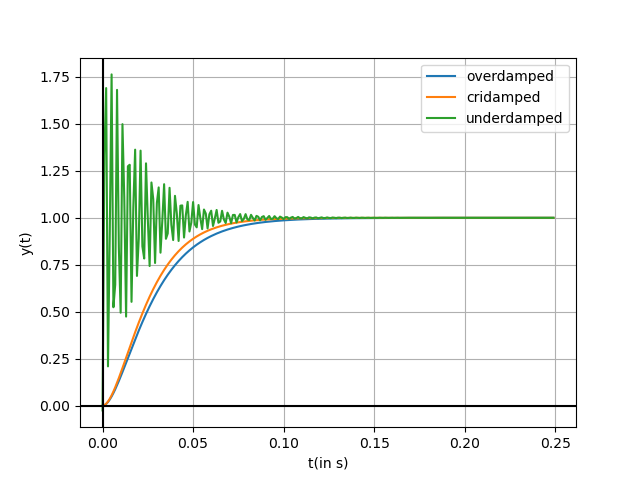
\includegraphics[width = \columnwidth]{app/figs/plot.png}
    \caption{Step response in all three cases}
\end{figure}

\end{enumerate}

\chapter{Analogous Systems}
\let\negmedspace\undefined
\let\negthickspace\undefined
\documentclass[journal,12pt,onecolumn]{IEEEtran}
\usepackage{cite}
\usepackage{amsmath,amssymb,amsfonts,amsthm}
\usepackage{algorithmic}
\usepackage{graphicx}
\usepackage{textcomp}
\usepackage{xcolor}
\usepackage{txfonts}
\usepackage{listings}
\usepackage{enumitem}
\usepackage{mathtools}
\usepackage{gensymb}
\usepackage[breaklinks=true]{hyperref}
\usepackage{tkz-euclide} % loads  TikZ and tkz-base
\usepackage{listings}



\newtheorem{theorem}{Theorem}[section]
\newtheorem{problem}{Problem}
\newtheorem{proposition}{Proposition}[section]
\newtheorem{lemma}{Lemma}[section]
\newtheorem{corollary}[theorem]{Corollary}
\newtheorem{example}{Example}[section]
\newtheorem{definition}[problem]{Definition}
%\newtheorem{thm}{Theorem}[section] 
%\newtheorem{defn}[thm]{Definition}
%\newtheorem{algorithm}{Algorithm}[section]
%\newtheorem{cor}{Corollary}
\newcommand{\BEQA}{\begin{eqnarray}}
\newcommand{\EEQA}{\end{eqnarray}}
\newcommand{\define}{\stackrel{\triangle}{=}}
\theoremstyle{remark}
\newtheorem{rem}{Remark}
%\bibliographystyle{ieeetr}
\begin{document}
%
\providecommand{\pr}[1]{\ensuremath{\Pr\left(#1\right)}}
\providecommand{\prt}[2]{\ensuremath{p_{#1}^{\left(#2\right)} }}        % own macro for this question
\providecommand{\qfunc}[1]{\ensuremath{Q\left(#1\right)}}
\providecommand{\sbrak}[1]{\ensuremath{{}\left[#1\right]}}
\providecommand{\lsbrak}[1]{\ensuremath{{}\left[#1\right.}}
\providecommand{\rsbrak}[1]{\ensuremath{{}\left.#1\right]}}
\providecommand{\brak}[1]{\ensuremath{\left(#1\right)}}
\providecommand{\lbrak}[1]{\ensuremath{\left(#1\right.}}
\providecommand{\rbrak}[1]{\ensuremath{\left.#1\right)}}
\providecommand{\cbrak}[1]{\ensuremath{\left\{#1\right\}}}
\providecommand{\lcbrak}[1]{\ensuremath{\left\{#1\right.}}
\providecommand{\rcbrak}[1]{\ensuremath{\left.#1\right\}}}
\newcommand{\sgn}{\mathop{\mathrm{sgn}}}
\providecommand{\abs}[1]{\left\vert#1\right\vert}
\providecommand{\res}[1]{\Res\displaylimits_{#1}} 
\providecommand{\norm}[1]{\left\lVert#1\right\rVert}
%\providecommand{\norm}[1]{\lVert#1\rVert}
\providecommand{\mtx}[1]{\mathbf{#1}}
\providecommand{\mean}[1]{E\left[ #1 \right]}
\providecommand{\cond}[2]{#1\middle|#2}
\providecommand{\fourier}{\overset{\mathcal{F}}{ \rightleftharpoons}}
\newenvironment{amatrix}[1]{%
  \left(\begin{array}{@{}*{#1}{c}|c@{}}
}{%
  \end{array}\right)
}
%\providecommand{\hilbert}{\overset{\mathcal{H}}{ \rightleftharpoons}}
%\providecommand{\system}{\overset{\mathcal{H}}{ \longleftrightarrow}}
	%\newcommand{\solution}[2]{\textbf{Solution:}{#1}}
\newcommand{\solution}{\noindent \textbf{Solution: }}
\newcommand{\cosec}{\,\text{cosec}\,}
\providecommand{\dec}[2]{\ensuremath{\overset{#1}{\underset{#2}{\gtrless}}}}
\newcommand{\myvec}[1]{\ensuremath{\begin{pmatrix}#1\end{pmatrix}}}
\newcommand{\mydet}[1]{\ensuremath{\begin{vmatrix}#1\end{vmatrix}}}
\newcommand{\myaugvec}[2]{\ensuremath{\begin{amatrix}{#1}#2\end{amatrix}}}
\providecommand{\rank}{\text{rank}}
\providecommand{\pr}[1]{\ensuremath{\Pr\left(#1\right)}}
\providecommand{\qfunc}[1]{\ensuremath{Q\left(#1\right)}}
	\newcommand*{\permcomb}[4][0mu]{{{}^{#3}\mkern#1#2_{#4}}}
\newcommand*{\perm}[1][-3mu]{\permcomb[#1]{P}}
\newcommand*{\comb}[1][-1mu]{\permcomb[#1]{C}}
\providecommand{\qfunc}[1]{\ensuremath{Q\left(#1\right)}}
\providecommand{\gauss}[2]{\mathcal{N}\ensuremath{\left(#1,#2\right)}}
\providecommand{\diff}[2]{\ensuremath{\frac{d{#1}}{d{#2}}}}
\providecommand{\myceil}[1]{\left \lceil #1 \right \rceil }
\newcommand\figref{Fig.~\ref}
\newcommand{\systemL}[1]{\stackrel{#1}{\xleftrightarrow{\mathcal{L}}}}
\newcommand{\systemLinv}[1]{\stackrel{#1}{\xleftrightarrow{\mathcal{L}^{-1}}}}


\newcommand\tabref{Table~\ref}
\newcommand{\sinc}{\,\text{sinc}\,}
\newcommand{\rect}{\,\text{rect}\,}
%%
%	%\newcommand{\solution}[2]{\textbf{Solution:}{#1}}
%\newcommand{\solution}{\noindent \textbf{Solution: }}
%\newcommand{\cosec}{\,\text{cosec}\,}
%\numberwithin{equation}{section}
%\numberwithin{equation}{subsection}
%\numberwithin{problem}{section}
%\numberwithin{definition}{section}
%\makeatletter
%\@addtoreset{figure}{problem}
%\makeatother

%\let\StandardTheFigure\thefigure
\let\vec\mathbf


\bibliographystyle{IEEEtran}
\title{ APPENDIX FOR ANALOGOUS SYSTEMS}
\author{EE23BTECH11011- Batchu Ishitha$^{*}$% <-this % stops a space
}
\maketitle




\bigskip

\renewcommand{\thefigure}{\theenumi}
\renewcommand{\thetable}{\theenumi}
%\renewcommand{\theequation}{\theenumi}

Analogous systems of electrical-mechanical systems are like a common language that bridges the gap between electrical and mechanical engineering. They allow us to understand and predict how different components interact, whether they're electrical circuits or mechanical machines. By recognizing similarities between electrical and mechanical elements, engineers can solve problems more efficiently and design better systems. This approach encourages collaboration between specialists from different fields and helps us develop innovative solutions that seamlessly integrate both electrical and mechanical aspects. \\

ELECTRICAL ANALOGIES OF MECHANICAL SYSTEMS:\\

Two systems are said to be analogous if :
\begin{enumerate}
\item The two systems are physically different.
\item Differential equation modelling of these two systems are same.
\end{enumerate} 


There are two types of electrical analogies of translational mechanical systems:
\begin{enumerate}
\item Force-Voltage analogy
\item Force-Current analogy
\end{enumerate} 

FORCE-VOLTAGE ANALOGY:\\
In this, the mathematical equations of translational mechanical system are compared with mesh equations of the electrical system.


\begin{table}[!ht]    
    \centering
     \begin{tabular}{|c|c|} 
    \hline
\textbf{Translational Mechanical System} & \textbf{Electrical System}  \\\hline
    Force(F) & Voltage(V)  \\\hline
    Mass(M) & Inductance (L) \\\hline
    Frictional coefficient(B) & Resistance(R) \\ \hline
    Spring constant(K) & Reciprocal of Capacitance(1/C)  \\\hline
    Displacement(x) & Charge(q) \\ \hline
    Velocity(v) & Current(i)  \\\hline
        \end{tabular}
    
 
      \caption{Input Parameters}
    \label{table:ishitha.g22.nm.54.at1}
\end{table}


Example: 
\begin{figure}[!ht]
    \centering
    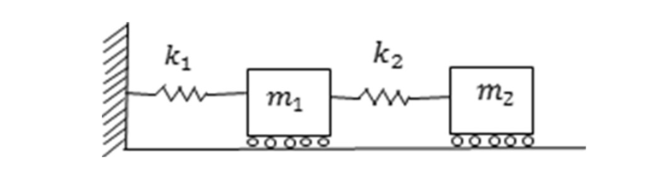
\includegraphics[scale=0.5]{app/figs/g54.fig1.png}
    \caption{ }
    \label{fig:ishitha.g22.nm.54.af1}
\end{figure}  


Equations of translational mechanical system:\\

\begin{figure}[!ht]
    \centering
    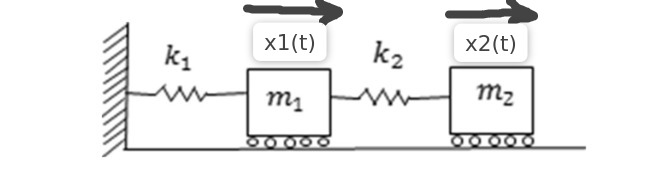
\includegraphics[scale=0.5]{app/figs/g54.fig2.jpeg}
    \caption{ }
    \label{fig:ishitha.g22.nm.54.af2}
\end{figure} 


\begin{align}
m_1\ddot{x_1}(t) - k_2\brak{x_2(t)-x_1(t)}+ k_1x_1(t)&=0
\label{eq:ishitha.g22.nm.54.1.eq}\\
m_2\ddot{x_2}(t) + k_2\brak{x_2(t)-x_1(t)}&=0
\label{eq:ishitha.g22.nm.54.2.eq} 
\end{align}

Mesh equations of electrical system:\\   

\begin{figure}[!ht]
    \centering
    \includegraphics[scale=1.5]{app/figs/tikz.pdf}
    \caption{ }
    \label{fig:ishitha.g22.nm.54.af3}
\end{figure}   
\begin{align}
 k_1\int i_1 \, dt + L_1\frac{di_1}{dt}+k_2\int \brak{i_1-i_2} \, dt &=0\\
 L_2\frac{di_2}{dt}-k_2\int \brak{i_1-i_2} \, dt &=0
\end{align}    

but we know, $i=\frac{dq}{dt}$ 
 \begin{align}
 \implies L_1\ddot q_1 -k_2\brak{q_2-q_1} + k_1q_1  &=0 \\
 \implies L_2\ddot q_2+k_2\brak{q_2-q_1} \, dt &=0
\end{align}  

FORCE-CURRENT ANALOGY:\\
In this , the mathematical equations of the translational mechanical system are compared with the nodal equations of the electrical system.


\begin{table}[!ht]    
    \centering
     \begin{tabular}{|c|c|} 
    \hline
\textbf{Translational Mechanical System} & \textbf{Electrical System}  \\\hline
    Force(F) &Current(i) \\\hline
    Mass(M) & Capacitance(C) \\\hline
    Frictional coefficient(B) &Reciprocal of Resistance(1/R) \\ \hline
    Spring constant(K) & Reciprocal of Inductance(1/L)  \\\hline
    Displacement(x) & Magnetic Flux($\psi $)\\ \hline
    Velocity(v) &  Voltage(V) \\\hline
        \end{tabular}
    
 
    \label{table:ishitha.g22.nm.54.at2}
\end{table}


\chapter{Frequency Response}
\begin{enumerate}[label=\thechapter.\arabic*,ref=\thechapter.\theenumi]
\numberwithin{equation}{enumi}
\numberwithin{figure}{enumi}
\numberwithin{table}{enumi}

\item \begin{figure}[!ht]
    \centering
    \begin{circuitikz}
   \draw(0,0) to [R](2,0);
   % \draw (2,0) -- (2.5,0);
   \draw(2,0) to [L] (4,0);
   % \draw (5,0) to (5,0);
   \draw (4,0) to [C] (4,-2);
   \draw(4,-2)  to (0,-2);
   \draw (4,0) -- (5,0);
   \draw (4,-2)to (5,-2);
   \node[circle,fill,inner sep=1pt] at (0,0) {};
   \node[circle,fill,inner sep=1pt] at (5,0) {};
   \node[circle,fill,inner sep=1pt] at (5,-2) {};
   \node[circle,fill,inner sep=1pt] at (0,-2) {};
   \draw[->](0,-1.85) to (0,-0.15);
   \draw[->](5,-1.85) to (5,-0.15);
   \node at (0.3,-1) {$x(t)$};
   \node at (5.5,-1) {$y(t)$};

   \node at (1,0.5) {$R$};
   \node at (3,0.5) {$L$};
   \node at (2.8,-1) {$C$};\node[circle,fill,inner sep=1pt] at (0,0) {};
\end{circuitikz}

    \caption{RLC Low pass filter}
\end{figure}
The frequency response $y_{ss}(t)$ is defined as the steady state response to a sinusoidal input signal $x(t) = \sin{\omega t}$. It describes how well the filter can distinguish between different frequencies.
\begin{align}
y_{ss}(t)=\abs{H(j\omega)}\,\sin(\omega t+\angle H(j\omega))
\end{align}
\begin{enumerate}
    \item Overdamped Case
    \begin{align}
        H(s)=\omega_0^2\frac{1}{(s-p_1)(s-p_2)}
    \end{align}
    where,
    \begin{align}
        p_{1,2} &= -\frac{R}{2L} \pm \sqrt{\left(\frac{R}{2L}\right)^2-\frac{1}{LC}}\\
         H(s) &= \abs{H(s)}\ e^{j\angle{H(s)}}\\
         \abs{H(s)} &= \omega_0^2 \frac{1}{\abs{s-p_1}\abs{s-p_2}}\\
         &=\omega_0^2\frac{1}{\left|j\omega-p_2\right|\,\left|j\omega-p_2\right|} \\
         &= \omega_0^2 \frac{1}{\sqrt{\omega^2+{p_1}^2}\sqrt{\omega^2+{p_2}^2}}\\
         \angle H(s) &= -(\angle(s-p_1)+\angle(s-p_2))\\
         &= \tan^{-1}\frac{\omega}{p_1} + \tan^{-1}\frac{\omega}{p_2}
    \end{align}
    The magnitude of the transfer function expressed on a logarithmic scale:
    \begin{multline}
        \abs{H_{dB}(\omega)} = 20\log(\omega_0^2) -20\log\sqrt{\omega^2+{p_1}^2}  \\
        -20\log\sqrt{\omega^2+{p_2}^2}
    \end{multline}

    \item Critically damped case
    \begin{align}
        H(s)=\omega_0^2\frac{1}{(s-p)^2}
    \end{align}
    where,
    \begin{align}
        p &=\sqrt{\frac{1}{LC}}\\
        H(s) &= \abs{H(s)}\ e^{j\angle{H(s)}}\\
        \abs{H(s)} &= \omega_0^2 \frac{1}{\abs{s-p}^2}\\
        \abs{H(j\omega)} &=\omega_0^2 \frac{1}{\abs{j\omega-p}^2}\\
        &=\omega_0^2\frac{1}{\omega^2+p^2}\\
        \angle H(s) &= -(\angle(s-p)+\angle(s-p))\\
         &= 2\tan^{-1}\frac{\omega}{p}
    \end{align}
    The magnitude of the transfer function expressed on a logarithmic scale:
    \begin{align}
        \abs{H_{dB}(\omega)} = 20\log(\omega_0^2) -20\log(\omega^2+{p}^2)
    \end{align}

    \item Underdamped Case
    \begin{align}
        H(s)=\omega_0^2\frac{1}{(s-p)(s-p^\ast)}
    \end{align}
    where,
    \begin{align}
        p,\,p^\ast &=\omega_n\brak{-\zeta \pm j\sqrt{1-\zeta^2}}\\
        &= -\sigma\pm j\omega_d\\
        H(s) &= \abs{H(s)}\ e^{j\angle{H(s)}}\\
        \abs{H(s)} &= \omega_0^2\frac{1}{\sqrt{({\omega_n}^2-\omega^2)^2+(2\zeta\omega_n \omega)^2}}\\
        \angle H(s) &= -(\angle(s-p)+\angle(s-p^*))\\
         &= -\tan^{-1}\frac{\omega+\omega_d}{\sigma} - \tan^{-1}\frac{\omega-\omega_d}{\sigma}
    \end{align}
    The magnitude of the transfer function expressed on a logarithmic scale:
    \begin{multline}
        \abs{H_{dB}(\omega)} = 20\log(\omega_0^2) \\-10\log(({\omega_n}^2-\omega^2)^2+(2\zeta\omega_n \omega)^2)
    \end{multline}
\end{enumerate}
\begin{figure}[!ht]
    \centering
    \includegraphics[width=\columnwidth]{app/figs/h_db_plot.png}
    \caption{Frequency response of all cases}
\end{figure}

\begin{figure}[!ht]
    \centering
    \includegraphics[width=\columnwidth]{app/figs/angle_H_s.png}
    \caption{Plot of $\angle H(s)$}
\end{figure}

\end{enumerate}


\iffalse
\chapter{ Convolution}
\chapter{ Z-transform}
\fi
\latexprintindex
\end{document}

 
